\documentclass[twoside]{book}

% Packages required by doxygen
\usepackage{fixltx2e}
\usepackage{calc}
\usepackage{doxygen}
\usepackage[export]{adjustbox} % also loads graphicx
\usepackage{graphicx}
\usepackage[utf8]{inputenc}
\usepackage{makeidx}
\usepackage{multicol}
\usepackage{multirow}
\PassOptionsToPackage{warn}{textcomp}
\usepackage{textcomp}
\usepackage[nointegrals]{wasysym}
\usepackage[table]{xcolor}

% Font selection
\usepackage[T1]{fontenc}
\usepackage[scaled=.90]{helvet}
\usepackage{courier}
\usepackage{amssymb}
\usepackage{sectsty}
\renewcommand{\familydefault}{\sfdefault}
\allsectionsfont{%
  \fontseries{bc}\selectfont%
  \color{darkgray}%
}
\renewcommand{\DoxyLabelFont}{%
  \fontseries{bc}\selectfont%
  \color{darkgray}%
}
\newcommand{\+}{\discretionary{\mbox{\scriptsize$\hookleftarrow$}}{}{}}

% Page & text layout
\usepackage{geometry}
\geometry{%
  a4paper,%
  top=2.5cm,%
  bottom=2.5cm,%
  left=2.5cm,%
  right=2.5cm%
}
\tolerance=750
\hfuzz=15pt
\hbadness=750
\setlength{\emergencystretch}{15pt}
\setlength{\parindent}{0cm}
\setlength{\parskip}{3ex plus 2ex minus 2ex}
\makeatletter
\renewcommand{\paragraph}{%
  \@startsection{paragraph}{4}{0ex}{-1.0ex}{1.0ex}{%
    \normalfont\normalsize\bfseries\SS@parafont%
  }%
}
\renewcommand{\subparagraph}{%
  \@startsection{subparagraph}{5}{0ex}{-1.0ex}{1.0ex}{%
    \normalfont\normalsize\bfseries\SS@subparafont%
  }%
}
\makeatother

% Headers & footers
\usepackage{fancyhdr}
\pagestyle{fancyplain}
\fancyhead[LE]{\fancyplain{}{\bfseries\thepage}}
\fancyhead[CE]{\fancyplain{}{}}
\fancyhead[RE]{\fancyplain{}{\bfseries\leftmark}}
\fancyhead[LO]{\fancyplain{}{\bfseries\rightmark}}
\fancyhead[CO]{\fancyplain{}{}}
\fancyhead[RO]{\fancyplain{}{\bfseries\thepage}}
\fancyfoot[LE]{\fancyplain{}{}}
\fancyfoot[CE]{\fancyplain{}{}}
\fancyfoot[RE]{\fancyplain{}{\bfseries\scriptsize Generated by Doxygen }}
\fancyfoot[LO]{\fancyplain{}{\bfseries\scriptsize Generated by Doxygen }}
\fancyfoot[CO]{\fancyplain{}{}}
\fancyfoot[RO]{\fancyplain{}{}}
\renewcommand{\footrulewidth}{0.4pt}
\renewcommand{\chaptermark}[1]{%
  \markboth{#1}{}%
}
\renewcommand{\sectionmark}[1]{%
  \markright{\thesection\ #1}%
}

% Indices & bibliography
\usepackage{natbib}
\usepackage[titles]{tocloft}
\setcounter{tocdepth}{3}
\setcounter{secnumdepth}{5}
\makeindex

% Hyperlinks (required, but should be loaded last)
\usepackage{ifpdf}
\ifpdf
  \usepackage[pdftex,pagebackref=true]{hyperref}
\else
  \usepackage[ps2pdf,pagebackref=true]{hyperref}
\fi
\hypersetup{%
  colorlinks=true,%
  linkcolor=blue,%
  citecolor=blue,%
  unicode%
}

% Custom commands
\newcommand{\clearemptydoublepage}{%
  \newpage{\pagestyle{empty}\cleardoublepage}%
}

\usepackage{caption}
\captionsetup{labelsep=space,justification=centering,font={bf},singlelinecheck=off,skip=4pt,position=top}

%===== C O N T E N T S =====

\begin{document}

% Titlepage & ToC
\hypersetup{pageanchor=false,
             bookmarksnumbered=true,
             pdfencoding=unicode
            }
\pagenumbering{alph}
\begin{titlepage}
\vspace*{7cm}
\begin{center}%
{\Large libomexmeta \\[1ex]\large 1.\+1.\+11 }\\
\vspace*{1cm}
{\large Generated by Doxygen 1.8.13}\\
\end{center}
\end{titlepage}
\clearemptydoublepage
\pagenumbering{roman}
\tableofcontents
\clearemptydoublepage
\pagenumbering{arabic}
\hypersetup{pageanchor=true}

%--- Begin generated contents ---
\chapter{Hierarchical Index}
\doxysection{Class Hierarchy}
This inheritance list is sorted roughly, but not completely, alphabetically\+:\begin{DoxyCompactList}
\item \contentsline{section}{copy}{\pageref{classcopy}}{}
\item \contentsline{section}{copy}{\pageref{classcopy}}{}
\item \contentsline{section}{omexmeta\+::Curl\+Get}{\pageref{classomexmeta_1_1CurlGet}}{}
\item \contentsline{section}{dbg\+::Debug\+Output}{\pageref{classdbg_1_1DebugOutput}}{}
\item \contentsline{section}{dbg\+::detail\+\_\+detector\+::detector$<$ Default, Always\+Void, Op, Args $>$}{\pageref{structdbg_1_1detail__detector_1_1detector}}{}
\item \contentsline{section}{dbg\+::detail\+\_\+detector\+::detector$<$ Default, void\+\_\+t$<$ Op$<$ Args... $>$ $>$, Op, Args... $>$}{\pageref{structdbg_1_1detail__detector_1_1detector_3_01Default_00_01void__t_3_01Op_3_01Args_8_8_8_01_4_01_4_00_01Op_00_01Args_8_8_8_01_4}}{}
\item \contentsline{section}{omexmeta\+::Editor}{\pageref{classomexmeta_1_1Editor}}{}
\item \contentsline{section}{omexmeta\+::Element\+Extractor}{\pageref{classomexmeta_1_1ElementExtractor}}{}
\item exception\begin{DoxyCompactList}
\item \contentsline{section}{Exception}{\pageref{classException}}{}
\begin{DoxyCompactList}
\item \contentsline{section}{Redland\+Librdf\+Exception}{\pageref{classRedlandLibrdfException}}{}
\item \contentsline{section}{Redland\+Null\+Pointer\+Exception}{\pageref{classRedlandNullPointerException}}{}
\end{DoxyCompactList}
\item \contentsline{section}{omexmeta\+::Exception}{\pageref{classomexmeta_1_1Exception}}{}
\begin{DoxyCompactList}
\item \contentsline{section}{omexmeta\+::Annotation\+Builder\+Exception}{\pageref{classomexmeta_1_1AnnotationBuilderException}}{}
\item \contentsline{section}{omexmeta\+::Inappropriate\+Resource\+Exception}{\pageref{classomexmeta_1_1InappropriateResourceException}}{}
\item \contentsline{section}{omexmeta\+::Lib\+R\+D\+F\+Exception}{\pageref{classomexmeta_1_1LibRDFException}}{}
\item \contentsline{section}{omexmeta\+::Not\+Implemented\+Exception}{\pageref{classomexmeta_1_1NotImplementedException}}{}
\item \contentsline{section}{omexmeta\+::Null\+Pointer\+Exception}{\pageref{classomexmeta_1_1NullPointerException}}{}
\item \contentsline{section}{omexmeta\+::Value\+Exception}{\pageref{classomexmeta_1_1ValueException}}{}
\end{DoxyCompactList}
\end{DoxyCompactList}
\item \contentsline{section}{omexmeta\+::I\+R\+DF}{\pageref{classomexmeta_1_1IRDF}}{}
\begin{DoxyCompactList}
\item \contentsline{section}{omexmeta\+::R\+DF}{\pageref{classomexmeta_1_1RDF}}{}
\end{DoxyCompactList}
\item \contentsline{section}{dbg\+::detail\+::is\+\_\+container$<$ T $>$}{\pageref{structdbg_1_1detail_1_1is__container}}{}
\item is\+\_\+detected\begin{DoxyCompactList}
\item \contentsline{section}{dbg\+::detail\+::has\+\_\+ostream\+\_\+operator$<$ T $>$}{\pageref{structdbg_1_1detail_1_1has__ostream__operator}}{}
\end{DoxyCompactList}
\item \contentsline{section}{dbg\+::last$<$ T, U $>$}{\pageref{structdbg_1_1last}}{}
\item \contentsline{section}{dbg\+::last$<$ T $>$}{\pageref{structdbg_1_1last_3_01T_01_4}}{}
\item \contentsline{section}{redland\+::Librdf\+Model}{\pageref{classredland_1_1LibrdfModel}}{}
\item \contentsline{section}{redland\+::Librdf\+Node}{\pageref{classredland_1_1LibrdfNode}}{}
\item \contentsline{section}{redland\+::Librdf\+Parser}{\pageref{classredland_1_1LibrdfParser}}{}
\item \contentsline{section}{redland\+::Librdf\+Query}{\pageref{classredland_1_1LibrdfQuery}}{}
\item \contentsline{section}{redland\+::Librdf\+Query\+Results}{\pageref{classredland_1_1LibrdfQueryResults}}{}
\item \contentsline{section}{redland\+::Librdf\+Serializer}{\pageref{classredland_1_1LibrdfSerializer}}{}
\item \contentsline{section}{redland\+::Librdf\+Statement}{\pageref{classredland_1_1LibrdfStatement}}{}
\begin{DoxyCompactList}
\item \contentsline{section}{omexmeta\+::Triple}{\pageref{classomexmeta_1_1Triple}}{}
\end{DoxyCompactList}
\item \contentsline{section}{redland\+::Librdf\+Storage}{\pageref{classredland_1_1LibrdfStorage}}{}
\item \contentsline{section}{redland\+::Librdf\+Stream}{\pageref{classredland_1_1LibrdfStream}}{}
\item \contentsline{section}{redland\+::Librdf\+Uri}{\pageref{classredland_1_1LibrdfUri}}{}
\item \contentsline{section}{Log\+Data$<$ List $>$}{\pageref{structLogData}}{}
\item \contentsline{section}{omexmeta\+::Markup\+Identifier}{\pageref{classomexmeta_1_1MarkupIdentifier}}{}
\item \contentsline{section}{omexmeta\+::Meta\+ID}{\pageref{classomexmeta_1_1MetaID}}{}
\item \contentsline{section}{None}{\pageref{structNone}}{}
\item \contentsline{section}{dbg\+::detail\+\_\+detector\+::nonesuch}{\pageref{structdbg_1_1detail__detector_1_1nonesuch}}{}
\item \contentsline{section}{omexmeta\+::Omex\+Meta\+Utils}{\pageref{classomexmeta_1_1OmexMetaUtils}}{}
\item \contentsline{section}{omexmeta\+::Omex\+Meta\+Xml\+Assistant}{\pageref{classomexmeta_1_1OmexMetaXmlAssistant}}{}
\begin{DoxyCompactList}
\item \contentsline{section}{omexmeta\+::Cell\+M\+L\+Assistant}{\pageref{classomexmeta_1_1CellMLAssistant}}{}
\item \contentsline{section}{omexmeta\+::S\+B\+M\+L\+Assistant}{\pageref{classomexmeta_1_1SBMLAssistant}}{}
\end{DoxyCompactList}
\item \contentsline{section}{omexmeta\+::Omex\+Meta\+Xml\+Assistant\+Factory}{\pageref{classomexmeta_1_1OmexMetaXmlAssistantFactory}}{}
\item \contentsline{section}{Pair$<$ First, Second $>$}{\pageref{structPair}}{}
\item \contentsline{section}{omexmeta\+::Participant}{\pageref{classomexmeta_1_1Participant}}{}
\begin{DoxyCompactList}
\item \contentsline{section}{omexmeta\+::Mediator\+Participant}{\pageref{classomexmeta_1_1MediatorParticipant}}{}
\item \contentsline{section}{omexmeta\+::Sink\+Participant}{\pageref{classomexmeta_1_1SinkParticipant}}{}
\item \contentsline{section}{omexmeta\+::Source\+Participant}{\pageref{classomexmeta_1_1SourceParticipant}}{}
\end{DoxyCompactList}
\item \contentsline{section}{omexmeta\+::Personal\+Information}{\pageref{classomexmeta_1_1PersonalInformation}}{}
\item \contentsline{section}{omexmeta\+::Physical\+Property}{\pageref{classomexmeta_1_1PhysicalProperty}}{}
\item \contentsline{section}{omexmeta\+::Predicate}{\pageref{classomexmeta_1_1Predicate}}{}
\begin{DoxyCompactList}
\item \contentsline{section}{omexmeta\+::Biomodels\+Biology\+Qualifier}{\pageref{classomexmeta_1_1BiomodelsBiologyQualifier}}{}
\item \contentsline{section}{omexmeta\+::Biomodels\+Model\+Qualifier}{\pageref{classomexmeta_1_1BiomodelsModelQualifier}}{}
\item \contentsline{section}{omexmeta\+::D\+C\+Term}{\pageref{classomexmeta_1_1DCTerm}}{}
\item \contentsline{section}{omexmeta\+::Foaf}{\pageref{classomexmeta_1_1Foaf}}{}
\item \contentsline{section}{omexmeta\+::Sem\+Sim}{\pageref{classomexmeta_1_1SemSim}}{}
\end{DoxyCompactList}
\item \contentsline{section}{dbg\+::pretty\+\_\+print\+\_\+tuple$<$ Idx $>$}{\pageref{structdbg_1_1pretty__print__tuple}}{}
\item \contentsline{section}{dbg\+::pretty\+\_\+print\+\_\+tuple$<$ 0 $>$}{\pageref{structdbg_1_1pretty__print__tuple_3_010_01_4}}{}
\item \contentsline{section}{dbg\+::print\+\_\+formatted$<$ T $>$}{\pageref{structdbg_1_1print__formatted}}{}
\item \contentsline{section}{dbg\+::print\+\_\+type$<$ T $>$}{\pageref{structdbg_1_1print__type}}{}
\item \contentsline{section}{omexmeta\+::Property\+Bearer}{\pageref{classomexmeta_1_1PropertyBearer}}{}
\begin{DoxyCompactList}
\item \contentsline{section}{omexmeta\+::Energy\+Diff}{\pageref{classomexmeta_1_1EnergyDiff}}{}
\item \contentsline{section}{omexmeta\+::Physical\+Entity}{\pageref{classomexmeta_1_1PhysicalEntity}}{}
\item \contentsline{section}{omexmeta\+::Physical\+Process}{\pageref{classomexmeta_1_1PhysicalProcess}}{}
\end{DoxyCompactList}
\item \contentsline{section}{omexmeta\+::Purge\+R\+D\+F\+Bag}{\pageref{classomexmeta_1_1PurgeRDFBag}}{}
\item \contentsline{section}{omexmeta\+::Query}{\pageref{classomexmeta_1_1Query}}{}
\item \contentsline{section}{raptor\+\_\+locator}{\pageref{structraptor__locator}}{}
\item \contentsline{section}{raptor\+\_\+statement}{\pageref{structraptor__statement}}{}
\item \contentsline{section}{raptor\+\_\+syntax\+\_\+description}{\pageref{structraptor__syntax__description}}{}
\item \contentsline{section}{raptor\+\_\+term}{\pageref{structraptor__term}}{}
\item \contentsline{section}{raptor\+\_\+term\+\_\+blank\+\_\+value}{\pageref{structraptor__term__blank__value}}{}
\item \contentsline{section}{raptor\+\_\+term\+\_\+literal\+\_\+value}{\pageref{structraptor__term__literal__value}}{}
\item \contentsline{section}{raptor\+\_\+term\+\_\+value}{\pageref{unionraptor__term__value}}{}
\item \contentsline{section}{raptor\+\_\+type\+\_\+q}{\pageref{structraptor__type__q}}{}
\item \contentsline{section}{redland\+::Raptor\+I\+O\+Stream}{\pageref{classredland_1_1RaptorIOStream}}{}
\item \contentsline{section}{rasqal\+\_\+data\+\_\+graph}{\pageref{structrasqal__data__graph}}{}
\item \contentsline{section}{rasqal\+\_\+evaluation\+\_\+context}{\pageref{structrasqal__evaluation__context}}{}
\item \contentsline{section}{rasqal\+\_\+expression\+\_\+s}{\pageref{structrasqal__expression__s}}{}
\item \contentsline{section}{rasqal\+\_\+literal\+\_\+s}{\pageref{structrasqal__literal__s}}{}
\item \contentsline{section}{rasqal\+\_\+prefix}{\pageref{structrasqal__prefix}}{}
\item \contentsline{section}{rasqal\+\_\+triple}{\pageref{structrasqal__triple}}{}
\item \contentsline{section}{rasqal\+\_\+triple\+\_\+meta}{\pageref{structrasqal__triple__meta}}{}
\item \contentsline{section}{rasqal\+\_\+triples\+\_\+match\+\_\+s}{\pageref{structrasqal__triples__match__s}}{}
\item \contentsline{section}{rasqal\+\_\+triples\+\_\+source\+\_\+factory}{\pageref{structrasqal__triples__source__factory}}{}
\item \contentsline{section}{rasqal\+\_\+triples\+\_\+source\+\_\+s}{\pageref{structrasqal__triples__source__s}}{}
\item \contentsline{section}{rasqal\+\_\+update\+\_\+operation}{\pageref{structrasqal__update__operation}}{}
\item \contentsline{section}{rasqal\+\_\+variable}{\pageref{structrasqal__variable}}{}
\item \contentsline{section}{rasqal\+\_\+xsd\+\_\+date}{\pageref{structrasqal__xsd__date}}{}
\item \contentsline{section}{rasqal\+\_\+xsd\+\_\+datetime}{\pageref{structrasqal__xsd__datetime}}{}
\item \contentsline{section}{omexmeta\+::S\+B\+M\+L\+Semantic\+Extraction}{\pageref{classomexmeta_1_1SBMLSemanticExtraction}}{}
\item \contentsline{section}{Subclass}{\pageref{classSubclass}}{}
\item \contentsline{section}{Subclass}{\pageref{classSubclass}}{}
\item \contentsline{section}{Subclass}{\pageref{classSubclass}}{}
\item \contentsline{section}{Subclass}{\pageref{classSubclass}}{}
\item \contentsline{section}{Subclass}{\pageref{classSubclass}}{}
\item \contentsline{section}{This}{\pageref{classThis}}{}
\item \contentsline{section}{dbg\+::time}{\pageref{structdbg_1_1time}}{}
\item \contentsline{section}{omexmeta\+::Triples}{\pageref{classomexmeta_1_1Triples}}{}
\item \contentsline{section}{dbg\+::type\+\_\+tag$<$ T $>$}{\pageref{structdbg_1_1type__tag}}{}
\item \contentsline{section}{omexmeta\+::Uri\+Handler}{\pageref{classomexmeta_1_1UriHandler}}{}
\item \contentsline{section}{omexmeta\+::V\+Card\+Translator}{\pageref{classomexmeta_1_1VCardTranslator}}{}
\item \contentsline{section}{redland\+::World}{\pageref{classredland_1_1World}}{}
\end{DoxyCompactList}

\chapter{Class Index}
\doxysection{Class List}
Here are the classes, structs, unions and interfaces with brief descriptions\+:\begin{DoxyCompactList}
\item\contentsline{section}{\mbox{\hyperlink{classomexmeta_1_1AnnotationBuilderException}{omexmeta\+::\+Annotation\+Builder\+Exception}} }{\pageref{classomexmeta_1_1AnnotationBuilderException}}{}
\item\contentsline{section}{\mbox{\hyperlink{classomexmeta_1_1BiomodelsBiologyQualifier}{omexmeta\+::\+Biomodels\+Biology\+Qualifier}} }{\pageref{classomexmeta_1_1BiomodelsBiologyQualifier}}{}
\item\contentsline{section}{\mbox{\hyperlink{classomexmeta_1_1BiomodelsModelQualifier}{omexmeta\+::\+Biomodels\+Model\+Qualifier}} }{\pageref{classomexmeta_1_1BiomodelsModelQualifier}}{}
\item\contentsline{section}{\mbox{\hyperlink{classomexmeta_1_1CurlGet}{omexmeta\+::\+Curl\+Get}} \\*Use libcurl to download from url }{\pageref{classomexmeta_1_1CurlGet}}{}
\item\contentsline{section}{\mbox{\hyperlink{classomexmeta_1_1DCTerm}{omexmeta\+::\+DCTerm}} }{\pageref{classomexmeta_1_1DCTerm}}{}
\item\contentsline{section}{\mbox{\hyperlink{classdbg_1_1DebugOutput}{dbg\+::\+Debug\+Output}} }{\pageref{classdbg_1_1DebugOutput}}{}
\item\contentsline{section}{\mbox{\hyperlink{structdbg_1_1detail__detector_1_1detector}{dbg\+::detail\+\_\+detector\+::detector$<$ Default, Always\+Void, Op, Args $>$}} }{\pageref{structdbg_1_1detail__detector_1_1detector}}{}
\item\contentsline{section}{\mbox{\hyperlink{structdbg_1_1detail__detector_1_1detector_3_01Default_00_01void__t_3_01Op_3_01Args_8_8_8_01_4_01_4_00_01Op_00_01Args_8_8_8_01_4}{dbg\+::detail\+\_\+detector\+::detector$<$ Default, void\+\_\+t$<$ Op$<$ Args... $>$ $>$, Op, Args... $>$}} }{\pageref{structdbg_1_1detail__detector_1_1detector_3_01Default_00_01void__t_3_01Op_3_01Args_8_8_8_01_4_01_4_00_01Op_00_01Args_8_8_8_01_4}}{}
\item\contentsline{section}{\mbox{\hyperlink{classomexmeta_1_1Editor}{omexmeta\+::\+Editor}} \\*Add or change annotations in xml }{\pageref{classomexmeta_1_1Editor}}{}
\item\contentsline{section}{\mbox{\hyperlink{classomexmeta_1_1ElementExtractor}{omexmeta\+::\+Element\+Extractor}} \\*Extract all elements from a document with name and put into a list }{\pageref{classomexmeta_1_1ElementExtractor}}{}
\item\contentsline{section}{\mbox{\hyperlink{classomexmeta_1_1EnergyDiff}{omexmeta\+::\+Energy\+Diff}} }{\pageref{classomexmeta_1_1EnergyDiff}}{}
\item\contentsline{section}{\mbox{\hyperlink{classException}{Exception}} }{\pageref{classException}}{}
\item\contentsline{section}{\mbox{\hyperlink{classomexmeta_1_1Exception}{omexmeta\+::\+Exception}} \\*Https\+://stackoverflow.com/questions/8152720/correct-\/way-\/to-\/inherit-\/from-\/stdexception }{\pageref{classomexmeta_1_1Exception}}{}
\item\contentsline{section}{\mbox{\hyperlink{classomexmeta_1_1Foaf}{omexmeta\+::\+Foaf}} }{\pageref{classomexmeta_1_1Foaf}}{}
\item\contentsline{section}{\mbox{\hyperlink{structdbg_1_1detail_1_1has__ostream__operator}{dbg\+::detail\+::has\+\_\+ostream\+\_\+operator$<$ T $>$}} }{\pageref{structdbg_1_1detail_1_1has__ostream__operator}}{}
\item\contentsline{section}{\mbox{\hyperlink{classomexmeta_1_1InappropriateResourceException}{omexmeta\+::\+Inappropriate\+Resource\+Exception}} }{\pageref{classomexmeta_1_1InappropriateResourceException}}{}
\item\contentsline{section}{\mbox{\hyperlink{classomexmeta_1_1IRDF}{omexmeta\+::\+IRDF}} \\*Public interface for \mbox{\hyperlink{classomexmeta_1_1RDF}{RDF}} types }{\pageref{classomexmeta_1_1IRDF}}{}
\item\contentsline{section}{\mbox{\hyperlink{structdbg_1_1detail_1_1is__container}{dbg\+::detail\+::is\+\_\+container$<$ T $>$}} }{\pageref{structdbg_1_1detail_1_1is__container}}{}
\item\contentsline{section}{\mbox{\hyperlink{structdbg_1_1last}{dbg\+::last$<$ T, U $>$}} }{\pageref{structdbg_1_1last}}{}
\item\contentsline{section}{\mbox{\hyperlink{structdbg_1_1last_3_01T_01_4}{dbg\+::last$<$ T $>$}} }{\pageref{structdbg_1_1last_3_01T_01_4}}{}
\item\contentsline{section}{\mbox{\hyperlink{classomexmeta_1_1LibRDFException}{omexmeta\+::\+Lib\+RDFException}} }{\pageref{classomexmeta_1_1LibRDFException}}{}
\item\contentsline{section}{\mbox{\hyperlink{classredland_1_1LibrdfModel}{redland\+::\+Librdf\+Model}} \\*RAII abstraction around librdf\+\_\+model }{\pageref{classredland_1_1LibrdfModel}}{}
\item\contentsline{section}{\mbox{\hyperlink{classredland_1_1LibrdfNode}{redland\+::\+Librdf\+Node}} \\*C++ wrapper around librdf\+\_\+node that uses RAII for memory management }{\pageref{classredland_1_1LibrdfNode}}{}
\item\contentsline{section}{\mbox{\hyperlink{classredland_1_1LibrdfParser}{redland\+::\+Librdf\+Parser}} }{\pageref{classredland_1_1LibrdfParser}}{}
\item\contentsline{section}{\mbox{\hyperlink{classredland_1_1LibrdfQuery}{redland\+::\+Librdf\+Query}} }{\pageref{classredland_1_1LibrdfQuery}}{}
\item\contentsline{section}{\mbox{\hyperlink{classredland_1_1LibrdfQueryResults}{redland\+::\+Librdf\+Query\+Results}} }{\pageref{classredland_1_1LibrdfQueryResults}}{}
\item\contentsline{section}{\mbox{\hyperlink{classredland_1_1LibrdfSerializer}{redland\+::\+Librdf\+Serializer}} }{\pageref{classredland_1_1LibrdfSerializer}}{}
\item\contentsline{section}{\mbox{\hyperlink{classredland_1_1LibrdfStatement}{redland\+::\+Librdf\+Statement}} \\*C++ wrapper around librdf\+\_\+statement using RAII for memory management }{\pageref{classredland_1_1LibrdfStatement}}{}
\item\contentsline{section}{\mbox{\hyperlink{classredland_1_1LibrdfStorage}{redland\+::\+Librdf\+Storage}} }{\pageref{classredland_1_1LibrdfStorage}}{}
\item\contentsline{section}{\mbox{\hyperlink{classredland_1_1LibrdfStream}{redland\+::\+Librdf\+Stream}} }{\pageref{classredland_1_1LibrdfStream}}{}
\item\contentsline{section}{\mbox{\hyperlink{classredland_1_1LibrdfUri}{redland\+::\+Librdf\+Uri}} \\*C++ wrapper around librdf\+\_\+uri using RAII }{\pageref{classredland_1_1LibrdfUri}}{}
\item\contentsline{section}{\mbox{\hyperlink{classredland_1_1LibrdfWorld}{redland\+::\+Librdf\+World}} }{\pageref{classredland_1_1LibrdfWorld}}{}
\item\contentsline{section}{\mbox{\hyperlink{classredland_1_1Logger}{redland\+::\+Logger}} \\*Logging class for lib\+Omex\+Meta. Implemented as a singleton }{\pageref{classredland_1_1Logger}}{}
\item\contentsline{section}{\mbox{\hyperlink{classomexmeta_1_1MarkupIdentifier}{omexmeta\+::\+Markup\+Identifier}} \\*Determines whether input language is sbml, cellml or unknown }{\pageref{classomexmeta_1_1MarkupIdentifier}}{}
\item\contentsline{section}{\mbox{\hyperlink{classomexmeta_1_1MediatorParticipant}{omexmeta\+::\+Mediator\+Participant}} }{\pageref{classomexmeta_1_1MediatorParticipant}}{}
\item\contentsline{section}{\mbox{\hyperlink{classomexmeta_1_1MetaID}{omexmeta\+::\+Meta\+ID}} \\*ID generator }{\pageref{classomexmeta_1_1MetaID}}{}
\item\contentsline{section}{\mbox{\hyperlink{structdbg_1_1detail__detector_1_1nonesuch}{dbg\+::detail\+\_\+detector\+::nonesuch}} }{\pageref{structdbg_1_1detail__detector_1_1nonesuch}}{}
\item\contentsline{section}{\mbox{\hyperlink{classomexmeta_1_1NotImplementedException}{omexmeta\+::\+Not\+Implemented\+Exception}} }{\pageref{classomexmeta_1_1NotImplementedException}}{}
\item\contentsline{section}{\mbox{\hyperlink{classomexmeta_1_1NullPointerException}{omexmeta\+::\+Null\+Pointer\+Exception}} }{\pageref{classomexmeta_1_1NullPointerException}}{}
\item\contentsline{section}{\mbox{\hyperlink{classomexmeta_1_1OmexMetaCellML}{omexmeta\+::\+Omex\+Meta\+Cell\+ML}} }{\pageref{classomexmeta_1_1OmexMetaCellML}}{}
\item\contentsline{section}{\mbox{\hyperlink{classomexmeta_1_1OmexMetaSBML}{omexmeta\+::\+Omex\+Meta\+SBML}} }{\pageref{classomexmeta_1_1OmexMetaSBML}}{}
\item\contentsline{section}{\mbox{\hyperlink{classomexmeta_1_1OmexMetaUtils}{omexmeta\+::\+Omex\+Meta\+Utils}} }{\pageref{classomexmeta_1_1OmexMetaUtils}}{}
\item\contentsline{section}{\mbox{\hyperlink{classomexmeta_1_1OmexMetaXml}{omexmeta\+::\+Omex\+Meta\+Xml}} \\*Construct for handling xml }{\pageref{classomexmeta_1_1OmexMetaXml}}{}
\item\contentsline{section}{\mbox{\hyperlink{classomexmeta_1_1OmexMetaXmlFactory}{omexmeta\+::\+Omex\+Meta\+Xml\+Factory}} }{\pageref{classomexmeta_1_1OmexMetaXmlFactory}}{}
\item\contentsline{section}{\mbox{\hyperlink{classOptions}{Options}} \\*Global options for lib\+Omex\+Meta }{\pageref{classOptions}}{}
\item\contentsline{section}{\mbox{\hyperlink{classomexmeta_1_1Participant}{omexmeta\+::\+Participant}} }{\pageref{classomexmeta_1_1Participant}}{}
\item\contentsline{section}{\mbox{\hyperlink{classomexmeta_1_1PersonalInformation}{omexmeta\+::\+Personal\+Information}} \\*Add personal information to the model as a composite annotation }{\pageref{classomexmeta_1_1PersonalInformation}}{}
\item\contentsline{section}{\mbox{\hyperlink{classomexmeta_1_1PhysicalEntity}{omexmeta\+::\+Physical\+Entity}} }{\pageref{classomexmeta_1_1PhysicalEntity}}{}
\item\contentsline{section}{\mbox{\hyperlink{classomexmeta_1_1PhysicalProcess}{omexmeta\+::\+Physical\+Process}} }{\pageref{classomexmeta_1_1PhysicalProcess}}{}
\item\contentsline{section}{\mbox{\hyperlink{classomexmeta_1_1PhysicalProperty}{omexmeta\+::\+Physical\+Property}} }{\pageref{classomexmeta_1_1PhysicalProperty}}{}
\item\contentsline{section}{\mbox{\hyperlink{classomexmeta_1_1Predicate}{omexmeta\+::\+Predicate}} }{\pageref{classomexmeta_1_1Predicate}}{}
\item\contentsline{section}{\mbox{\hyperlink{structdbg_1_1pretty__print__tuple}{dbg\+::pretty\+\_\+print\+\_\+tuple$<$ Idx $>$}} }{\pageref{structdbg_1_1pretty__print__tuple}}{}
\item\contentsline{section}{\mbox{\hyperlink{structdbg_1_1pretty__print__tuple_3_010_01_4}{dbg\+::pretty\+\_\+print\+\_\+tuple$<$ 0 $>$}} }{\pageref{structdbg_1_1pretty__print__tuple_3_010_01_4}}{}
\item\contentsline{section}{\mbox{\hyperlink{structdbg_1_1print__formatted}{dbg\+::print\+\_\+formatted$<$ T $>$}} }{\pageref{structdbg_1_1print__formatted}}{}
\item\contentsline{section}{\mbox{\hyperlink{structdbg_1_1print__type}{dbg\+::print\+\_\+type$<$ T $>$}} }{\pageref{structdbg_1_1print__type}}{}
\item\contentsline{section}{\mbox{\hyperlink{classomexmeta_1_1PropertyBearer}{omexmeta\+::\+Property\+Bearer}} }{\pageref{classomexmeta_1_1PropertyBearer}}{}
\item\contentsline{section}{\mbox{\hyperlink{classomexmeta_1_1PurgeRDFBag}{omexmeta\+::\+Purge\+RDFBag}} }{\pageref{classomexmeta_1_1PurgeRDFBag}}{}
\item\contentsline{section}{\mbox{\hyperlink{classomexmeta_1_1Query}{omexmeta\+::\+Query}} \\*Make a Sparql }{\pageref{classomexmeta_1_1Query}}{}
\item\contentsline{section}{\mbox{\hyperlink{structraptor__locator}{raptor\+\_\+locator}} }{\pageref{structraptor__locator}}{}
\item\contentsline{section}{\mbox{\hyperlink{structraptor__statement}{raptor\+\_\+statement}} }{\pageref{structraptor__statement}}{}
\item\contentsline{section}{\mbox{\hyperlink{structraptor__syntax__description}{raptor\+\_\+syntax\+\_\+description}} }{\pageref{structraptor__syntax__description}}{}
\item\contentsline{section}{\mbox{\hyperlink{structraptor__term}{raptor\+\_\+term}} }{\pageref{structraptor__term}}{}
\item\contentsline{section}{\mbox{\hyperlink{structraptor__term__blank__value}{raptor\+\_\+term\+\_\+blank\+\_\+value}} }{\pageref{structraptor__term__blank__value}}{}
\item\contentsline{section}{\mbox{\hyperlink{structraptor__term__literal__value}{raptor\+\_\+term\+\_\+literal\+\_\+value}} }{\pageref{structraptor__term__literal__value}}{}
\item\contentsline{section}{\mbox{\hyperlink{unionraptor__term__value}{raptor\+\_\+term\+\_\+value}} }{\pageref{unionraptor__term__value}}{}
\item\contentsline{section}{\mbox{\hyperlink{structraptor__type__q}{raptor\+\_\+type\+\_\+q}} }{\pageref{structraptor__type__q}}{}
\item\contentsline{section}{\mbox{\hyperlink{structraptor__uri__s}{raptor\+\_\+uri\+\_\+s}} }{\pageref{structraptor__uri__s}}{}
\item\contentsline{section}{\mbox{\hyperlink{classredland_1_1RaptorIOStream}{redland\+::\+Raptor\+IOStream}} }{\pageref{classredland_1_1RaptorIOStream}}{}
\item\contentsline{section}{\mbox{\hyperlink{structrasqal__data__graph}{rasqal\+\_\+data\+\_\+graph}} }{\pageref{structrasqal__data__graph}}{}
\item\contentsline{section}{\mbox{\hyperlink{structrasqal__evaluation__context}{rasqal\+\_\+evaluation\+\_\+context}} }{\pageref{structrasqal__evaluation__context}}{}
\item\contentsline{section}{\mbox{\hyperlink{structrasqal__expression__s}{rasqal\+\_\+expression\+\_\+s}} }{\pageref{structrasqal__expression__s}}{}
\item\contentsline{section}{\mbox{\hyperlink{structrasqal__literal__s}{rasqal\+\_\+literal\+\_\+s}} }{\pageref{structrasqal__literal__s}}{}
\item\contentsline{section}{\mbox{\hyperlink{structrasqal__prefix}{rasqal\+\_\+prefix}} }{\pageref{structrasqal__prefix}}{}
\item\contentsline{section}{\mbox{\hyperlink{structrasqal__triple}{rasqal\+\_\+triple}} }{\pageref{structrasqal__triple}}{}
\item\contentsline{section}{\mbox{\hyperlink{structrasqal__triple__meta}{rasqal\+\_\+triple\+\_\+meta}} }{\pageref{structrasqal__triple__meta}}{}
\item\contentsline{section}{\mbox{\hyperlink{structrasqal__triples__match__s}{rasqal\+\_\+triples\+\_\+match\+\_\+s}} }{\pageref{structrasqal__triples__match__s}}{}
\item\contentsline{section}{\mbox{\hyperlink{structrasqal__triples__source__factory}{rasqal\+\_\+triples\+\_\+source\+\_\+factory}} }{\pageref{structrasqal__triples__source__factory}}{}
\item\contentsline{section}{\mbox{\hyperlink{structrasqal__triples__source__s}{rasqal\+\_\+triples\+\_\+source\+\_\+s}} }{\pageref{structrasqal__triples__source__s}}{}
\item\contentsline{section}{\mbox{\hyperlink{structrasqal__update__operation}{rasqal\+\_\+update\+\_\+operation}} }{\pageref{structrasqal__update__operation}}{}
\item\contentsline{section}{\mbox{\hyperlink{structrasqal__variable}{rasqal\+\_\+variable}} }{\pageref{structrasqal__variable}}{}
\item\contentsline{section}{\mbox{\hyperlink{structrasqal__xsd__date}{rasqal\+\_\+xsd\+\_\+date}} }{\pageref{structrasqal__xsd__date}}{}
\item\contentsline{section}{\mbox{\hyperlink{structrasqal__xsd__datetime}{rasqal\+\_\+xsd\+\_\+datetime}} }{\pageref{structrasqal__xsd__datetime}}{}
\item\contentsline{section}{\mbox{\hyperlink{classomexmeta_1_1RDF}{omexmeta\+::\+RDF}} }{\pageref{classomexmeta_1_1RDF}}{}
\item\contentsline{section}{\mbox{\hyperlink{classRedlandLibrdfException}{Redland\+Librdf\+Exception}} }{\pageref{classRedlandLibrdfException}}{}
\item\contentsline{section}{\mbox{\hyperlink{classRedlandNullPointerException}{Redland\+Null\+Pointer\+Exception}} }{\pageref{classRedlandNullPointerException}}{}
\item\contentsline{section}{\mbox{\hyperlink{classredland_1_1RedlandType}{redland\+::\+Redland\+Type$<$ Obj\+Type, Free\+Func\+Type $>$}} }{\pageref{classredland_1_1RedlandType}}{}
\item\contentsline{section}{\mbox{\hyperlink{classredland_1_1RefCountedRedlandType}{redland\+::\+Ref\+Counted\+Redland\+Type$<$ Obj\+Type, Free\+Func\+Type $>$}} }{\pageref{classredland_1_1RefCountedRedlandType}}{}
\item\contentsline{section}{\mbox{\hyperlink{classomexmeta_1_1SBMLSemanticExtraction}{omexmeta\+::\+SBMLSemantic\+Extraction}} }{\pageref{classomexmeta_1_1SBMLSemanticExtraction}}{}
\item\contentsline{section}{\mbox{\hyperlink{classomexmeta_1_1SemSim}{omexmeta\+::\+Sem\+Sim}} }{\pageref{classomexmeta_1_1SemSim}}{}
\item\contentsline{section}{\mbox{\hyperlink{classomexmeta_1_1SinkParticipant}{omexmeta\+::\+Sink\+Participant}} }{\pageref{classomexmeta_1_1SinkParticipant}}{}
\item\contentsline{section}{\mbox{\hyperlink{classomexmeta_1_1SourceParticipant}{omexmeta\+::\+Source\+Participant}} }{\pageref{classomexmeta_1_1SourceParticipant}}{}
\item\contentsline{section}{\mbox{\hyperlink{classSubclass}{Subclass}} }{\pageref{classSubclass}}{}
\item\contentsline{section}{\mbox{\hyperlink{classThis}{This}} \\*Interface for querying an rdf graph basically a wrapper around both librdf\+\_\+query and librdf\+\_\+query\+\_\+results. Query is not used by users directly but accessed indurectly without the users knowledge via the RDF\+::query method. Query results can be returned in 1 of 9 formats\+: }{\pageref{classThis}}{}
\item\contentsline{section}{\mbox{\hyperlink{structdbg_1_1time}{dbg\+::time}} }{\pageref{structdbg_1_1time}}{}
\item\contentsline{section}{\mbox{\hyperlink{classomexmeta_1_1Triple}{omexmeta\+::\+Triple}} }{\pageref{classomexmeta_1_1Triple}}{}
\item\contentsline{section}{\mbox{\hyperlink{classomexmeta_1_1Triples}{omexmeta\+::\+Triples}} \\*A \mbox{\hyperlink{classomexmeta_1_1Triples}{Triples}} object is a collection of \mbox{\hyperlink{classomexmeta_1_1Triple}{Triple}} objects }{\pageref{classomexmeta_1_1Triples}}{}
\item\contentsline{section}{\mbox{\hyperlink{structdbg_1_1type__tag}{dbg\+::type\+\_\+tag$<$ T $>$}} }{\pageref{structdbg_1_1type__tag}}{}
\item\contentsline{section}{\mbox{\hyperlink{classomexmeta_1_1UriHandler}{omexmeta\+::\+Uri\+Handler}} }{\pageref{classomexmeta_1_1UriHandler}}{}
\item\contentsline{section}{\mbox{\hyperlink{classomexmeta_1_1ValueException}{omexmeta\+::\+Value\+Exception}} }{\pageref{classomexmeta_1_1ValueException}}{}
\item\contentsline{section}{\mbox{\hyperlink{classomexmeta_1_1VCardTranslator}{omexmeta\+::\+VCard\+Translator}} }{\pageref{classomexmeta_1_1VCardTranslator}}{}
\end{DoxyCompactList}

\chapter{Class Documentation}
\hypertarget{classomexmeta_1_1AnnotationBuilderException}{}\doxysection{omexmeta\+::Annotation\+Builder\+Exception Class Reference}
\label{classomexmeta_1_1AnnotationBuilderException}\index{omexmeta::AnnotationBuilderException@{omexmeta::AnnotationBuilderException}}
Inheritance diagram for omexmeta\+::Annotation\+Builder\+Exception\+:\begin{figure}[H]
\begin{center}
\leavevmode
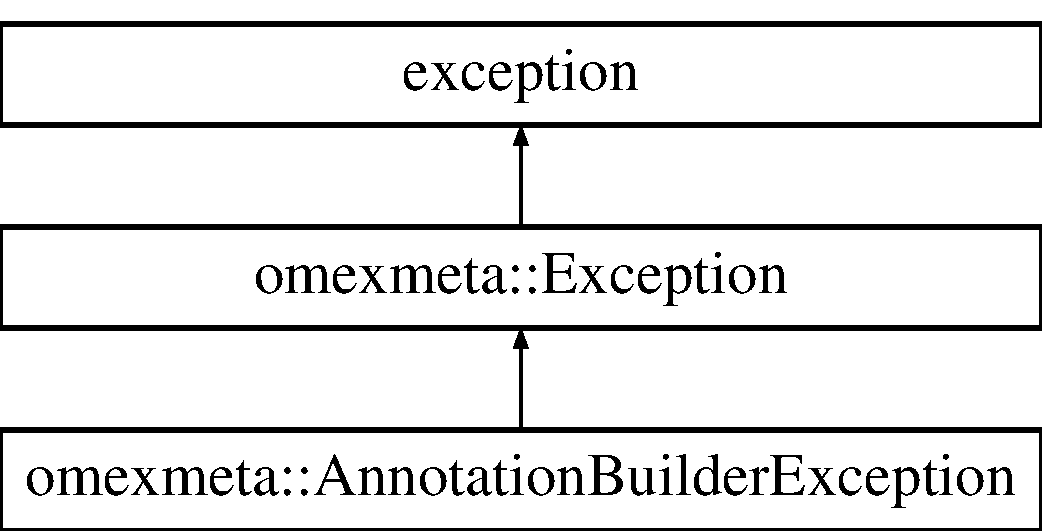
\includegraphics[height=3.000000cm]{classomexmeta_1_1AnnotationBuilderException}
\end{center}
\end{figure}
\doxysubsection*{Additional Inherited Members}


The documentation for this class was generated from the following file\+:\begin{DoxyCompactItemize}
\item 
src/omexmeta/Error.\+h\end{DoxyCompactItemize}

\hypertarget{classomexmeta_1_1BiomodelsBiologyQualifier}{}\doxysection{omexmeta\+::Biomodels\+Biology\+Qualifier Class Reference}
\label{classomexmeta_1_1BiomodelsBiologyQualifier}\index{omexmeta::BiomodelsBiologyQualifier@{omexmeta::BiomodelsBiologyQualifier}}
Inheritance diagram for omexmeta\+::Biomodels\+Biology\+Qualifier\+:\begin{figure}[H]
\begin{center}
\leavevmode
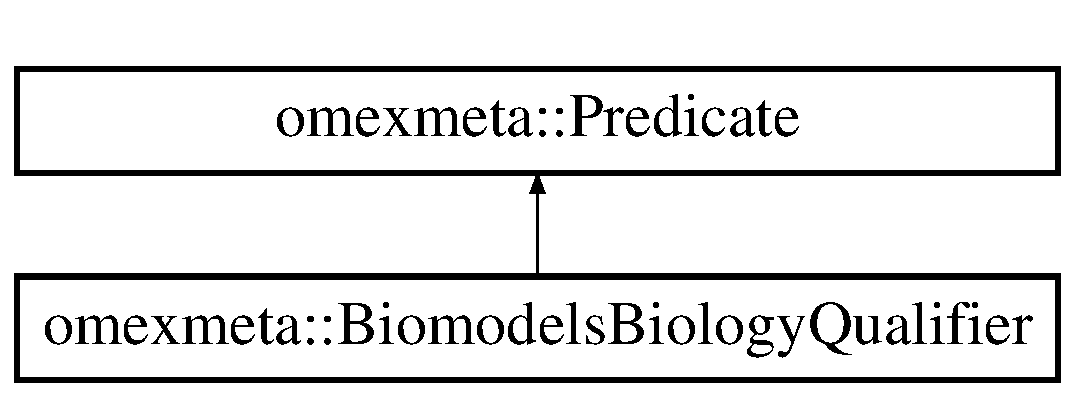
\includegraphics[height=2.000000cm]{classomexmeta_1_1BiomodelsBiologyQualifier}
\end{center}
\end{figure}
\doxysubsection*{Public Member Functions}
\begin{DoxyCompactItemize}
\item 
\mbox{\hyperlink{classomexmeta_1_1BiomodelsBiologyQualifier_a4dfa8fd975ceba60da6d3ccabdfb4514}{Biomodels\+Biology\+Qualifier}} (const std\+::string \&term)
\item 
\mbox{\Hypertarget{classomexmeta_1_1BiomodelsBiologyQualifier_ade9766c18afa895e7c745aa4679ccfce}\label{classomexmeta_1_1BiomodelsBiologyQualifier_ade9766c18afa895e7c745aa4679ccfce}} 
void {\bfseries verify} ()
\end{DoxyCompactItemize}
\doxysubsection*{Public Attributes}
\begin{DoxyCompactItemize}
\item 
std\+::vector$<$ std\+::string $>$ {\bfseries valid\+\_\+terms\+\_\+}
\end{DoxyCompactItemize}
\doxysubsection*{Additional Inherited Members}


\doxysubsection{Constructor \& Destructor Documentation}
\mbox{\Hypertarget{classomexmeta_1_1BiomodelsBiologyQualifier_a4dfa8fd975ceba60da6d3ccabdfb4514}\label{classomexmeta_1_1BiomodelsBiologyQualifier_a4dfa8fd975ceba60da6d3ccabdfb4514}} 
\index{omexmeta::BiomodelsBiologyQualifier@{omexmeta::BiomodelsBiologyQualifier}!BiomodelsBiologyQualifier@{BiomodelsBiologyQualifier}}
\index{BiomodelsBiologyQualifier@{BiomodelsBiologyQualifier}!omexmeta::BiomodelsBiologyQualifier@{omexmeta::BiomodelsBiologyQualifier}}
\doxysubsubsection{\texorpdfstring{BiomodelsBiologyQualifier()}{BiomodelsBiologyQualifier()}}
{\footnotesize\ttfamily omexmeta\+::\+Biomodels\+Biology\+Qualifier\+::\+Biomodels\+Biology\+Qualifier (\begin{DoxyParamCaption}\item[{const std\+::string \&}]{term }\end{DoxyParamCaption})\hspace{0.3cm}{\ttfamily [explicit]}}

note\+: verify cannot be a virtual function because I want to use it in the constructor. Therefore, I made \mbox{\hyperlink{classomexmeta_1_1Predicate_a1e7e59b8a48c9f89eeec73f3bbaea19c}{Predicate\+::verify}} static to reduce code duplication.

\doxysubsection{Member Data Documentation}
\mbox{\Hypertarget{classomexmeta_1_1BiomodelsBiologyQualifier_a5ae1a3da58f05beb1e8b389f36f486bf}\label{classomexmeta_1_1BiomodelsBiologyQualifier_a5ae1a3da58f05beb1e8b389f36f486bf}} 
\index{omexmeta::BiomodelsBiologyQualifier@{omexmeta::BiomodelsBiologyQualifier}!valid\_terms\_@{valid\_terms\_}}
\index{valid\_terms\_@{valid\_terms\_}!omexmeta::BiomodelsBiologyQualifier@{omexmeta::BiomodelsBiologyQualifier}}
\doxysubsubsection{\texorpdfstring{valid\_terms\_}{valid\_terms\_}}
{\footnotesize\ttfamily std\+::vector$<$std\+::string$>$ omexmeta\+::\+Biomodels\+Biology\+Qualifier\+::valid\+\_\+terms\+\_\+}

{\bfseries Initial value\+:}
\begin{DoxyCode}{0}
\DoxyCodeLine{\{}
\DoxyCodeLine{                \textcolor{stringliteral}{"{}is"{}},}
\DoxyCodeLine{                \textcolor{stringliteral}{"{}hasPart"{}},}
\DoxyCodeLine{                \textcolor{stringliteral}{"{}isPartOf"{}},}
\DoxyCodeLine{                \textcolor{stringliteral}{"{}isVersionOf"{}},}
\DoxyCodeLine{                \textcolor{stringliteral}{"{}hasVersion"{}},}
\DoxyCodeLine{                \textcolor{stringliteral}{"{}isHomologTo"{}},}
\DoxyCodeLine{                \textcolor{stringliteral}{"{}isDescribedBy"{}},}
\DoxyCodeLine{                \textcolor{stringliteral}{"{}isEncodedBy"{}},}
\DoxyCodeLine{                \textcolor{stringliteral}{"{}encodes"{}},}
\DoxyCodeLine{                \textcolor{stringliteral}{"{}occursIn"{}},}
\DoxyCodeLine{                \textcolor{stringliteral}{"{}hasProperty"{}},}
\DoxyCodeLine{                \textcolor{stringliteral}{"{}isPropertyOf"{}},}
\DoxyCodeLine{                \textcolor{stringliteral}{"{}hasTaxon"{}}}
\DoxyCodeLine{        \}}

\end{DoxyCode}


The documentation for this class was generated from the following files\+:\begin{DoxyCompactItemize}
\item 
src/omexmeta/Predicate.\+h\item 
src/omexmeta/Predicate.\+cpp\end{DoxyCompactItemize}

\hypertarget{classomexmeta_1_1BiomodelsModelQualifier}{}\doxysection{omexmeta\+::Biomodels\+Model\+Qualifier Class Reference}
\label{classomexmeta_1_1BiomodelsModelQualifier}\index{omexmeta::BiomodelsModelQualifier@{omexmeta::BiomodelsModelQualifier}}
Inheritance diagram for omexmeta\+::Biomodels\+Model\+Qualifier\+:\begin{figure}[H]
\begin{center}
\leavevmode
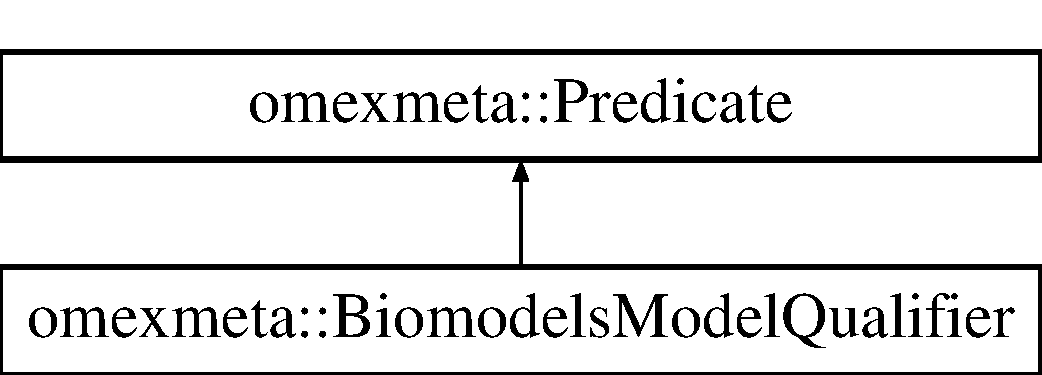
\includegraphics[height=2.000000cm]{classomexmeta_1_1BiomodelsModelQualifier}
\end{center}
\end{figure}
\doxysubsection*{Public Member Functions}
\begin{DoxyCompactItemize}
\item 
\mbox{\Hypertarget{classomexmeta_1_1BiomodelsModelQualifier_a9842d4d8aa136cf4d617a53e12dc6f82}\label{classomexmeta_1_1BiomodelsModelQualifier_a9842d4d8aa136cf4d617a53e12dc6f82}} 
{\bfseries Biomodels\+Model\+Qualifier} (const std\+::string \&term)
\item 
\mbox{\Hypertarget{classomexmeta_1_1BiomodelsModelQualifier_a3d55d1629ea82f6bb20068818b462fee}\label{classomexmeta_1_1BiomodelsModelQualifier_a3d55d1629ea82f6bb20068818b462fee}} 
void {\bfseries verify} ()
\end{DoxyCompactItemize}
\doxysubsection*{Public Attributes}
\begin{DoxyCompactItemize}
\item 
std\+::vector$<$ std\+::string $>$ {\bfseries valid\+\_\+terms\+\_\+}
\end{DoxyCompactItemize}
\doxysubsection*{Additional Inherited Members}


\doxysubsection{Member Data Documentation}
\mbox{\Hypertarget{classomexmeta_1_1BiomodelsModelQualifier_ab1d28ff2e7904f06b393a874f3d9607f}\label{classomexmeta_1_1BiomodelsModelQualifier_ab1d28ff2e7904f06b393a874f3d9607f}} 
\index{omexmeta::BiomodelsModelQualifier@{omexmeta::BiomodelsModelQualifier}!valid\_terms\_@{valid\_terms\_}}
\index{valid\_terms\_@{valid\_terms\_}!omexmeta::BiomodelsModelQualifier@{omexmeta::BiomodelsModelQualifier}}
\doxysubsubsection{\texorpdfstring{valid\_terms\_}{valid\_terms\_}}
{\footnotesize\ttfamily std\+::vector$<$std\+::string$>$ omexmeta\+::\+Biomodels\+Model\+Qualifier\+::valid\+\_\+terms\+\_\+}

{\bfseries Initial value\+:}
\begin{DoxyCode}{0}
\DoxyCodeLine{\{}
\DoxyCodeLine{                \textcolor{stringliteral}{"{}isDerivedFrom"{}},}
\DoxyCodeLine{                \textcolor{stringliteral}{"{}isDescribedBy"{}},}
\DoxyCodeLine{                \textcolor{stringliteral}{"{}isInstanceOf"{}},}
\DoxyCodeLine{                \textcolor{stringliteral}{"{}hasInstance"{}},}
\DoxyCodeLine{        \}}

\end{DoxyCode}


The documentation for this class was generated from the following files\+:\begin{DoxyCompactItemize}
\item 
src/omexmeta/include/omexmeta/Predicate.\+h\item 
src/omexmeta/Predicate.\+cpp\end{DoxyCompactItemize}

\hypertarget{classomexmeta_1_1CellMLAssistant}{}\doxysection{omexmeta\+::Cell\+M\+L\+Assistant Class Reference}
\label{classomexmeta_1_1CellMLAssistant}\index{omexmeta::CellMLAssistant@{omexmeta::CellMLAssistant}}
Inheritance diagram for omexmeta\+::Cell\+M\+L\+Assistant\+:\begin{figure}[H]
\begin{center}
\leavevmode
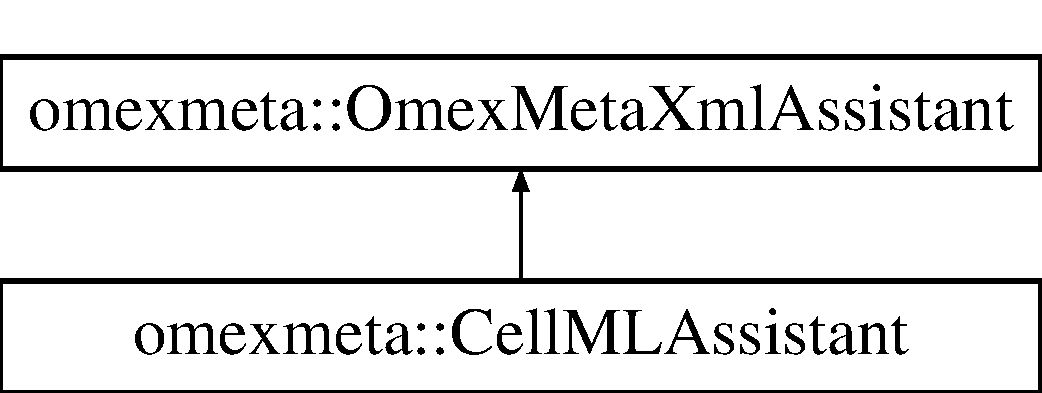
\includegraphics[height=2.000000cm]{classomexmeta_1_1CellMLAssistant}
\end{center}
\end{figure}
\doxysubsection*{Public Member Functions}
\begin{DoxyCompactItemize}
\item 
\mbox{\Hypertarget{classomexmeta_1_1CellMLAssistant_ad0fa4e23c94197d5682a0f8e1dec0889}\label{classomexmeta_1_1CellMLAssistant_ad0fa4e23c94197d5682a0f8e1dec0889}} 
std\+::vector$<$ std\+::string $>$ {\bfseries get\+Valid\+Elements} () const override
\item 
\mbox{\Hypertarget{classomexmeta_1_1CellMLAssistant_a4aaccf21ed47201abaf20d67ad7bfaab}\label{classomexmeta_1_1CellMLAssistant_a4aaccf21ed47201abaf20d67ad7bfaab}} 
std\+::string {\bfseries meta\+Id\+Tag\+Name} () const override
\item 
\mbox{\Hypertarget{classomexmeta_1_1CellMLAssistant_a856b49e96c2015b5445f6921d5738388}\label{classomexmeta_1_1CellMLAssistant_a856b49e96c2015b5445f6921d5738388}} 
std\+::string {\bfseries meta\+Id\+Namespace} () const override
\item 
\mbox{\Hypertarget{classomexmeta_1_1CellMLAssistant_af619a65dd28d04dfabd1930ff4110ce0}\label{classomexmeta_1_1CellMLAssistant_af619a65dd28d04dfabd1930ff4110ce0}} 
{\bfseries Omex\+Meta\+Xml\+Assistant} (std\+::string xml, std\+::string metaid\+\_\+base=\char`\"{}Meta\+ID\char`\"{}, int metaid\+\_\+num\+\_\+digits=4, bool generate\+\_\+new\+\_\+metaids=false)
\end{DoxyCompactItemize}


The documentation for this class was generated from the following files\+:\begin{DoxyCompactItemize}
\item 
src/omexmeta/include/omexmeta/Omex\+Meta\+Xml\+Assistant.\+h\item 
src/omexmeta/Omex\+Meta\+Xml\+Assistant.\+cpp\end{DoxyCompactItemize}

\hypertarget{classomexmeta_1_1CurlGet}{}\section{omexmeta\+:\+:Curl\+Get Class Reference}
\label{classomexmeta_1_1CurlGet}\index{omexmeta\+::\+Curl\+Get@{omexmeta\+::\+Curl\+Get}}


Use libcurl to download from url.  




{\ttfamily \#include $<$Curl\+Get.\+h$>$}

\subsection*{Static Public Member Functions}
\begin{DoxyCompactItemize}
\item 
static int \hyperlink{classomexmeta_1_1CurlGet_a52eaa2b1179cf49ec298022011b2477c}{download} (const std\+::string \&url, const std\+::string \&output\+\_\+filename)
\begin{DoxyCompactList}\small\item\em download a file from the internet \end{DoxyCompactList}\end{DoxyCompactItemize}


\subsection{Detailed Description}
Use libcurl to download from url. 

\subsection{Member Function Documentation}
\mbox{\Hypertarget{classomexmeta_1_1CurlGet_a52eaa2b1179cf49ec298022011b2477c}\label{classomexmeta_1_1CurlGet_a52eaa2b1179cf49ec298022011b2477c}} 
\index{omexmeta\+::\+Curl\+Get@{omexmeta\+::\+Curl\+Get}!download@{download}}
\index{download@{download}!omexmeta\+::\+Curl\+Get@{omexmeta\+::\+Curl\+Get}}
\subsubsection{\texorpdfstring{download()}{download()}}
{\footnotesize\ttfamily int omexmeta\+::\+Curl\+Get\+::download (\begin{DoxyParamCaption}\item[{const std\+::string \&}]{url,  }\item[{const std\+::string \&}]{output\+\_\+filename }\end{DoxyParamCaption})\hspace{0.3cm}{\ttfamily [static]}}



download a file from the internet 


\begin{DoxyParams}{Parameters}
{\em url} & The url to download. \\
\hline
{\em output\+\_\+filename.} & Where to put the downloaded content. \\
\hline
\end{DoxyParams}
\begin{DoxyReturn}{Returns}
success code. Non-\/0 fails. 
\end{DoxyReturn}


The documentation for this class was generated from the following files\+:\begin{DoxyCompactItemize}
\item 
src/omexmeta/Curl\+Get.\+h\item 
src/omexmeta/Curl\+Get.\+cpp\end{DoxyCompactItemize}

\hypertarget{classomexmeta_1_1DCTerm}{}\doxysection{omexmeta\+::D\+C\+Term Class Reference}
\label{classomexmeta_1_1DCTerm}\index{omexmeta::DCTerm@{omexmeta::DCTerm}}
Inheritance diagram for omexmeta\+::D\+C\+Term\+:\begin{figure}[H]
\begin{center}
\leavevmode
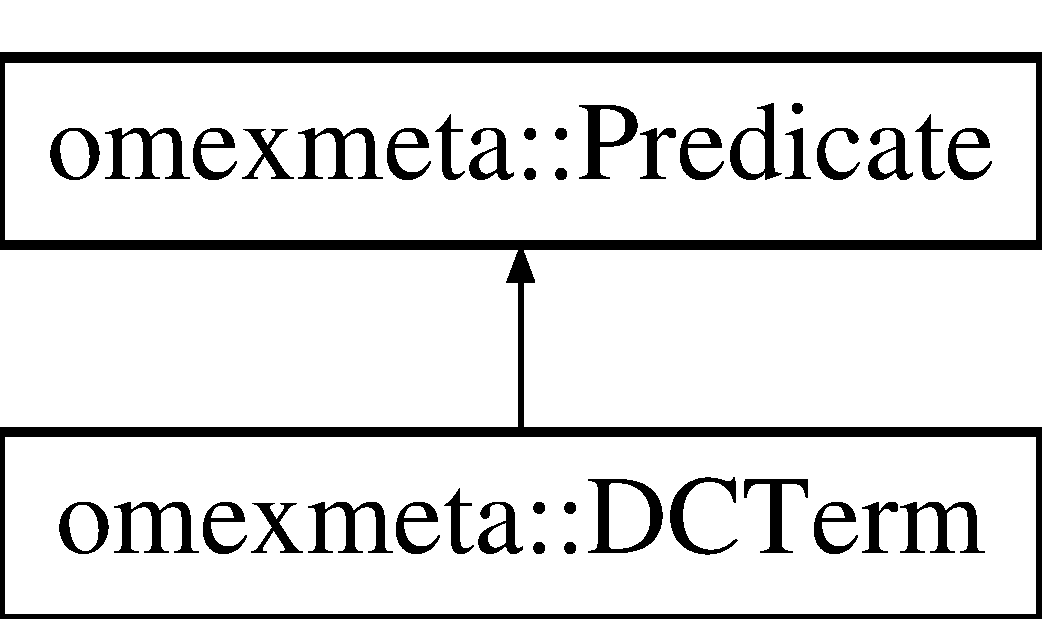
\includegraphics[height=2.000000cm]{classomexmeta_1_1DCTerm}
\end{center}
\end{figure}
\doxysubsection*{Public Member Functions}
\begin{DoxyCompactItemize}
\item 
\mbox{\Hypertarget{classomexmeta_1_1DCTerm_a114081e0845c3f4c306b881da2d065cd}\label{classomexmeta_1_1DCTerm_a114081e0845c3f4c306b881da2d065cd}} 
{\bfseries D\+C\+Term} (const std\+::string \&term)
\item 
\mbox{\Hypertarget{classomexmeta_1_1DCTerm_aae02242702d1bb360c0a1ebb4dae8126}\label{classomexmeta_1_1DCTerm_aae02242702d1bb360c0a1ebb4dae8126}} 
void {\bfseries verify} ()
\end{DoxyCompactItemize}
\doxysubsection*{Public Attributes}
\begin{DoxyCompactItemize}
\item 
std\+::vector$<$ std\+::string $>$ {\bfseries valid\+\_\+terms\+\_\+}
\end{DoxyCompactItemize}
\doxysubsection*{Additional Inherited Members}


\doxysubsection{Member Data Documentation}
\mbox{\Hypertarget{classomexmeta_1_1DCTerm_a3216c98de5a311d5f824dc132fefc3e4}\label{classomexmeta_1_1DCTerm_a3216c98de5a311d5f824dc132fefc3e4}} 
\index{omexmeta::DCTerm@{omexmeta::DCTerm}!valid\_terms\_@{valid\_terms\_}}
\index{valid\_terms\_@{valid\_terms\_}!omexmeta::DCTerm@{omexmeta::DCTerm}}
\doxysubsubsection{\texorpdfstring{valid\_terms\_}{valid\_terms\_}}
{\footnotesize\ttfamily std\+::vector$<$std\+::string$>$ omexmeta\+::\+D\+C\+Term\+::valid\+\_\+terms\+\_\+}

{\bfseries Initial value\+:}
\begin{DoxyCode}{0}
\DoxyCodeLine{\{}
\DoxyCodeLine{                \textcolor{stringliteral}{"{}abstract"{}}, \textcolor{stringliteral}{"{}accessRights"{}}, \textcolor{stringliteral}{"{}accrualMethod"{}}, \textcolor{stringliteral}{"{}accrualPeriodicity"{}}, \textcolor{stringliteral}{"{}accrualPolicy"{}}, \textcolor{stringliteral}{"{}alternative"{}},}
\DoxyCodeLine{                \textcolor{stringliteral}{"{}audience"{}}, \textcolor{stringliteral}{"{}available"{}}, \textcolor{stringliteral}{"{}bibliographicCitation"{}}, \textcolor{stringliteral}{"{}conformsTo"{}}, \textcolor{stringliteral}{"{}contributor"{}}, \textcolor{stringliteral}{"{}coverage"{}}, \textcolor{stringliteral}{"{}created"{}},}
\DoxyCodeLine{                \textcolor{stringliteral}{"{}creator"{}}, \textcolor{stringliteral}{"{}date"{}}, \textcolor{stringliteral}{"{}dateAccepted"{}}, \textcolor{stringliteral}{"{}dateCopyrighted"{}}, \textcolor{stringliteral}{"{}dateSubmitted"{}}, \textcolor{stringliteral}{"{}description"{}}, \textcolor{stringliteral}{"{}educationLevel"{}},}
\DoxyCodeLine{                \textcolor{stringliteral}{"{}extent"{}}, \textcolor{stringliteral}{"{}format"{}}, \textcolor{stringliteral}{"{}hasFormat"{}}, \textcolor{stringliteral}{"{}hasPart"{}}, \textcolor{stringliteral}{"{}hasVersion"{}}, \textcolor{stringliteral}{"{}identifier"{}}, \textcolor{stringliteral}{"{}instructionalMethod"{}},}
\DoxyCodeLine{                \textcolor{stringliteral}{"{}isFormatOf"{}}, \textcolor{stringliteral}{"{}isPartOf"{}}, \textcolor{stringliteral}{"{}isReferencedBy"{}}, \textcolor{stringliteral}{"{}isReplacedBy"{}}, \textcolor{stringliteral}{"{}isRequiredBy"{}}, \textcolor{stringliteral}{"{}issued"{}}, \textcolor{stringliteral}{"{}isVersionOf"{}},}
\DoxyCodeLine{                \textcolor{stringliteral}{"{}language"{}}, \textcolor{stringliteral}{"{}license"{}}, \textcolor{stringliteral}{"{}mediator"{}}, \textcolor{stringliteral}{"{}medium"{}}, \textcolor{stringliteral}{"{}modified"{}}, \textcolor{stringliteral}{"{}provenance"{}}, \textcolor{stringliteral}{"{}publisher"{}}, \textcolor{stringliteral}{"{}references"{}},}
\DoxyCodeLine{                \textcolor{stringliteral}{"{}relation"{}}, \textcolor{stringliteral}{"{}replaces"{}}, \textcolor{stringliteral}{"{}requires"{}}, \textcolor{stringliteral}{"{}rights"{}}, \textcolor{stringliteral}{"{}rightsHolder"{}}, \textcolor{stringliteral}{"{}source"{}}, \textcolor{stringliteral}{"{}spatial"{}}, \textcolor{stringliteral}{"{}subject"{}},}
\DoxyCodeLine{                \textcolor{stringliteral}{"{}tableOfContents"{}}, \textcolor{stringliteral}{"{}temporal"{}}, \textcolor{stringliteral}{"{}title"{}}, \textcolor{stringliteral}{"{}type"{}}, \textcolor{stringliteral}{"{}valid"{}}, \textcolor{stringliteral}{"{}W3CDTF"{}}\}}

\end{DoxyCode}


The documentation for this class was generated from the following files\+:\begin{DoxyCompactItemize}
\item 
src/omexmeta/include/omexmeta/Predicate.\+h\item 
src/omexmeta/Predicate.\+cpp\end{DoxyCompactItemize}

\hypertarget{classdbg_1_1DebugOutput}{}\section{dbg\+:\+:Debug\+Output Class Reference}
\label{classdbg_1_1DebugOutput}\index{dbg\+::\+Debug\+Output@{dbg\+::\+Debug\+Output}}
\subsection*{Public Types}
\begin{DoxyCompactItemize}
\item 
\mbox{\Hypertarget{classdbg_1_1DebugOutput_a5d9b38d5b9276cb584c0e20e9b1a2045}\label{classdbg_1_1DebugOutput_a5d9b38d5b9276cb584c0e20e9b1a2045}} 
using {\bfseries expr\+\_\+t} = const char $\ast$
\end{DoxyCompactItemize}
\subsection*{Public Member Functions}
\begin{DoxyCompactItemize}
\item 
\mbox{\Hypertarget{classdbg_1_1DebugOutput_a7bb0378758aa1006e2423eff57ee36a2}\label{classdbg_1_1DebugOutput_a7bb0378758aa1006e2423eff57ee36a2}} 
{\bfseries Debug\+Output} (const char $\ast$filepath, int line, const char $\ast$function\+\_\+name)
\item 
\mbox{\Hypertarget{classdbg_1_1DebugOutput_aa135787802db4a6b0b4eb185185e13ca}\label{classdbg_1_1DebugOutput_aa135787802db4a6b0b4eb185185e13ca}} 
{\footnotesize template$<$typename... T$>$ }\\auto {\bfseries print} (std\+::initializer\+\_\+list$<$ expr\+\_\+t $>$ exprs, std\+::initializer\+\_\+list$<$ std\+::string $>$ types, T \&\&... values) -\/$>$ last\+\_\+t$<$ T... $>$
\end{DoxyCompactItemize}


The documentation for this class was generated from the following file\+:\begin{DoxyCompactItemize}
\item 
src/omexmeta/dbg.\+h\end{DoxyCompactItemize}

\hypertarget{structdbg_1_1detail__detector_1_1detector}{}\section{dbg\+:\+:detail\+\_\+detector\+:\+:detector$<$ Default, Always\+Void, Op, Args $>$ Struct Template Reference}
\label{structdbg_1_1detail__detector_1_1detector}\index{dbg\+::detail\+\_\+detector\+::detector$<$ Default, Always\+Void, Op, Args $>$@{dbg\+::detail\+\_\+detector\+::detector$<$ Default, Always\+Void, Op, Args $>$}}
\subsection*{Public Types}
\begin{DoxyCompactItemize}
\item 
\mbox{\Hypertarget{structdbg_1_1detail__detector_1_1detector_af1b6da4282d723669e926c52f446a989}\label{structdbg_1_1detail__detector_1_1detector_af1b6da4282d723669e926c52f446a989}} 
using {\bfseries value\+\_\+t} = std\+::false\+\_\+type
\item 
\mbox{\Hypertarget{structdbg_1_1detail__detector_1_1detector_aab6b446944545683b9533ea8fc623480}\label{structdbg_1_1detail__detector_1_1detector_aab6b446944545683b9533ea8fc623480}} 
using {\bfseries type} = Default
\end{DoxyCompactItemize}


The documentation for this struct was generated from the following file\+:\begin{DoxyCompactItemize}
\item 
src/omexmeta/dbg.\+h\end{DoxyCompactItemize}

\hypertarget{structdbg_1_1detail__detector_1_1detector_3_01Default_00_01void__t_3_01Op_3_01Args_8_8_8_01_4_01_4_00_01Op_00_01Args_8_8_8_01_4}{}\doxysection{dbg\+::detail\+\_\+detector\+::detector$<$ Default, void\+\_\+t$<$ Op$<$ Args... $>$ $>$, Op, Args... $>$ Struct Template Reference}
\label{structdbg_1_1detail__detector_1_1detector_3_01Default_00_01void__t_3_01Op_3_01Args_8_8_8_01_4_01_4_00_01Op_00_01Args_8_8_8_01_4}\index{dbg::detail\_detector::detector$<$ Default, void\_t$<$ Op$<$ Args... $>$ $>$, Op, Args... $>$@{dbg::detail\_detector::detector$<$ Default, void\_t$<$ Op$<$ Args... $>$ $>$, Op, Args... $>$}}
\doxysubsection*{Public Types}
\begin{DoxyCompactItemize}
\item 
\mbox{\Hypertarget{structdbg_1_1detail__detector_1_1detector_3_01Default_00_01void__t_3_01Op_3_01Args_8_8_8_01_4_01_4_00_01Op_00_01Args_8_8_8_01_4_ab9dc20c0565be267d2d98b0e0f4a565b}\label{structdbg_1_1detail__detector_1_1detector_3_01Default_00_01void__t_3_01Op_3_01Args_8_8_8_01_4_01_4_00_01Op_00_01Args_8_8_8_01_4_ab9dc20c0565be267d2d98b0e0f4a565b}} 
using {\bfseries value\+\_\+t} = std\+::true\+\_\+type
\item 
\mbox{\Hypertarget{structdbg_1_1detail__detector_1_1detector_3_01Default_00_01void__t_3_01Op_3_01Args_8_8_8_01_4_01_4_00_01Op_00_01Args_8_8_8_01_4_a2119ba35e684b8292286546a1cea10d1}\label{structdbg_1_1detail__detector_1_1detector_3_01Default_00_01void__t_3_01Op_3_01Args_8_8_8_01_4_01_4_00_01Op_00_01Args_8_8_8_01_4_a2119ba35e684b8292286546a1cea10d1}} 
using {\bfseries type} = Op$<$ Args... $>$
\end{DoxyCompactItemize}


The documentation for this struct was generated from the following file\+:\begin{DoxyCompactItemize}
\item 
src/omexmeta/include/omexmeta/dbg.\+h\end{DoxyCompactItemize}

\hypertarget{classomexmeta_1_1Editor}{}\doxysection{omexmeta\+::Editor Class Reference}
\label{classomexmeta_1_1Editor}\index{omexmeta::Editor@{omexmeta::Editor}}


Add or change annotations in xml.  




{\ttfamily \#include $<$Editor.\+h$>$}

\doxysubsection*{Public Member Functions}
\begin{DoxyCompactItemize}
\item 
\mbox{\hyperlink{classomexmeta_1_1Editor_a6ac976c1a3762f77a577b5735cd509f4}{Editor}} (const std\+::string \&xml, bool create\+\_\+ids, const \mbox{\hyperlink{classredland_1_1LibrdfModel}{Librdf\+Model}} \&model, Namespace\+Map \&ns\+\_\+map, bool generate\+\_\+new\+\_\+metaids=false, bool sbml\+\_\+semantic\+\_\+extraction=true, const std\+::string \&repository\+\_\+uri=std\+::string(), const std\+::string \&archive\+\_\+uri=std\+::string(), const std\+::string \&model\+\_\+uri=std\+::string(), const std\+::string \&local\+\_\+uri=std\+::string())
\begin{DoxyCompactList}\small\item\em constructor for \mbox{\hyperlink{classomexmeta_1_1Editor}{Editor}}. \end{DoxyCompactList}\item 
\mbox{\hyperlink{classomexmeta_1_1Editor_aa11380bb7e2ca7859937c3f5907b6240}{$\sim$\+Editor}} ()=default
\item 
\mbox{\Hypertarget{classomexmeta_1_1Editor_ab5b39f1f137312ce77575e73a86dfb05}\label{classomexmeta_1_1Editor_ab5b39f1f137312ce77575e73a86dfb05}} 
int {\bfseries size} () const
\item 
const Namespace\+Map \& \mbox{\hyperlink{classomexmeta_1_1Editor_a514443fe99a6e52154d1fe4f7ec94618}{get\+Namespaces}} () const
\begin{DoxyCompactList}\small\item\em returns a hashmap of namespaces to prefixes. \end{DoxyCompactList}\item 
librdf\+\_\+model $\ast$ \mbox{\hyperlink{classomexmeta_1_1Editor_a4b2610fb802eb306349d69ae6fde60c0}{get\+Model}} () const
\begin{DoxyCompactList}\small\item\em return the underlying librdf\+\_\+model$\ast$ pointer \end{DoxyCompactList}\item 
\mbox{\Hypertarget{classomexmeta_1_1Editor_a83836e19bb1de9c7df69d36e8b61b2b2}\label{classomexmeta_1_1Editor_a83836e19bb1de9c7df69d36e8b61b2b2}} 
void \mbox{\hyperlink{classomexmeta_1_1Editor_a83836e19bb1de9c7df69d36e8b61b2b2}{set\+Namespaces}} (const Namespace\+Map \&namespaces)
\begin{DoxyCompactList}\small\item\em set the namespace map. \end{DoxyCompactList}\item 
const std\+::string \& \mbox{\hyperlink{classomexmeta_1_1Editor_ad931e829fc9f78717e0c1443c619b7d3}{get\+Xml}} () const
\begin{DoxyCompactList}\small\item\em return the xml \end{DoxyCompactList}\item 
const std\+::vector$<$ std\+::string $>$ \& \mbox{\hyperlink{classomexmeta_1_1Editor_a242c86222e1aeff337d3af22641db1de}{get\+Metaids}} () const
\begin{DoxyCompactList}\small\item\em returns a list of metaids both that existed previously and that was added during instantiation. \end{DoxyCompactList}\item 
void \mbox{\hyperlink{classomexmeta_1_1Editor_a052a725cee8b8e577c55e977eee81ace}{add\+Namespace}} (const std\+::string \&ns, std\+::string prefix)
\begin{DoxyCompactList}\small\item\em add a namespace \end{DoxyCompactList}\item 
void \mbox{\hyperlink{classomexmeta_1_1Editor_a0417b55575a244817ef981f17c8e1a8f}{add\+Single\+Annotation}} (\mbox{\hyperlink{classomexmeta_1_1Subject}{Subject}} subject, const Predicate\+Ptr \&predicate\+\_\+ptr, const \mbox{\hyperlink{classomexmeta_1_1Resource}{Resource}} \&resource)
\begin{DoxyCompactList}\small\item\em Add a Single\+Annotation (aka a \mbox{\hyperlink{classomexmeta_1_1Triple}{Triple}}) to the model. \end{DoxyCompactList}\item 
void \mbox{\hyperlink{classomexmeta_1_1Editor_ae46835f3f35425d8087b80d08666aaa4}{add\+Single\+Annotation}} (\mbox{\hyperlink{classomexmeta_1_1Triple}{Singular\+Annotation}} \&singular\+Annotation)
\begin{DoxyCompactList}\small\item\em Add a Single\+Annotation (aka \mbox{\hyperlink{classomexmeta_1_1Triple}{Triple}}) to the rdf graph. \end{DoxyCompactList}\item 
void \mbox{\hyperlink{classomexmeta_1_1Editor_afcb5ce7397aab23fabd3b4b4b89d3a54}{remove\+Single\+Annotation}} (const \mbox{\hyperlink{classomexmeta_1_1Triple}{Singular\+Annotation}} \&singular\+Annotation) const
\begin{DoxyCompactList}\small\item\em remove a singular annotation (aka \mbox{\hyperlink{classomexmeta_1_1Triple}{Triple}}) from the rdf graph \end{DoxyCompactList}\item 
void \mbox{\hyperlink{classomexmeta_1_1Editor_a146ae84fb44991d9c6135e98f03fa972}{add\+Composite\+Annotation}} (\mbox{\hyperlink{classomexmeta_1_1PhysicalPhenomenon}{Physical\+Phenomenon}} $\ast$phenomenon\+Ptr)
\begin{DoxyCompactList}\small\item\em add a composite annotation to the rdf graph. \end{DoxyCompactList}\item 
void \mbox{\hyperlink{classomexmeta_1_1Editor_a0740831baafe244374ad7a324d51a87e}{add\+Physical\+Entity}} (\mbox{\hyperlink{classomexmeta_1_1PhysicalEntity}{Physical\+Entity}} \&physical\+Entity)
\begin{DoxyCompactList}\small\item\em add a composite annotation of type \mbox{\hyperlink{classomexmeta_1_1PhysicalEntity}{Physical\+Entity}} to the rdf graph \end{DoxyCompactList}\item 
void \mbox{\hyperlink{classomexmeta_1_1Editor_a0acf94314252b70a4db89f83e6047e8f}{remove\+Physical\+Entity}} (\mbox{\hyperlink{classomexmeta_1_1PhysicalEntity}{Physical\+Entity}} \&physical\+Entity) const
\begin{DoxyCompactList}\small\item\em remove triples associated with a a \mbox{\hyperlink{classomexmeta_1_1PhysicalEntity}{Physical\+Entity}} object from the rdf graph \end{DoxyCompactList}\item 
void \mbox{\hyperlink{classomexmeta_1_1Editor_a8be7fa01bef49ff1c93965781797c9bc}{remove\+Personal\+Information}} (\mbox{\hyperlink{classomexmeta_1_1PersonalInformation}{Personal\+Information}} $\ast$information) const
\begin{DoxyCompactList}\small\item\em remove triples associated with a \mbox{\hyperlink{classomexmeta_1_1PersonalInformation}{Personal\+Information}} object from the rdf graph \end{DoxyCompactList}\item 
void \mbox{\hyperlink{classomexmeta_1_1Editor_ae4a608ecbe64f05c1b64efbeeb1fdeb1}{add\+Physical\+Process}} (\mbox{\hyperlink{classomexmeta_1_1PhysicalProcess}{Physical\+Process}} \&physical\+Process)
\begin{DoxyCompactList}\small\item\em add a composite annotation of type \mbox{\hyperlink{classomexmeta_1_1PhysicalProcess}{Physical\+Process}} to the rdf graph \end{DoxyCompactList}\item 
void \mbox{\hyperlink{classomexmeta_1_1Editor_a42640d74c6afe780738c906bdf346a78}{remove\+Physical\+Process}} (\mbox{\hyperlink{classomexmeta_1_1PhysicalProcess}{Physical\+Process}} \&physical\+Process) const
\begin{DoxyCompactList}\small\item\em remove triples associated with a \mbox{\hyperlink{classomexmeta_1_1PhysicalProcess}{Physical\+Process}} object from the rdf graph \end{DoxyCompactList}\item 
void \mbox{\hyperlink{classomexmeta_1_1Editor_a7833e03995f6323109c2db8d59104f6c}{add\+Physical\+Force}} (\mbox{\hyperlink{classomexmeta_1_1PhysicalForce}{Physical\+Force}} \&physical\+Force)
\begin{DoxyCompactList}\small\item\em add a composite annotation of type \mbox{\hyperlink{classomexmeta_1_1PhysicalForce}{Physical\+Force}} to the rdf graph \end{DoxyCompactList}\item 
void \mbox{\hyperlink{classomexmeta_1_1Editor_a1b2e0f5859fe2e2784ecff2a78f7f1f8}{add\+Personal\+Information}} (\mbox{\hyperlink{classomexmeta_1_1PersonalInformation}{Personal\+Information}} $\ast$personal\+Information)
\begin{DoxyCompactList}\small\item\em add a \mbox{\hyperlink{classomexmeta_1_1PersonalInformation}{Personal\+Information}} class to the rdf model \end{DoxyCompactList}\item 
void \mbox{\hyperlink{classomexmeta_1_1Editor_ad99187ec52bef1af440af5d9560f32c5}{remove\+Physical\+Force}} (\mbox{\hyperlink{classomexmeta_1_1PhysicalForce}{Physical\+Force}} \&physical\+Force) const
\begin{DoxyCompactList}\small\item\em remove triples associated with a a \mbox{\hyperlink{classomexmeta_1_1PhysicalForce}{Physical\+Force}} object from the rdf graph \end{DoxyCompactList}\item 
\mbox{\Hypertarget{classomexmeta_1_1Editor_a790458ef32f01ce0a6fd87bf14bed81a}\label{classomexmeta_1_1Editor_a790458ef32f01ce0a6fd87bf14bed81a}} 
void \mbox{\hyperlink{classomexmeta_1_1Editor_a790458ef32f01ce0a6fd87bf14bed81a}{check\+Valid\+Metaid}} (const std\+::string \&metaid)
\begin{DoxyCompactList}\small\item\em check that a metaid is valid by comparing with the output from Editor\+::get\+Meta\+Ids() \end{DoxyCompactList}\item 
\mbox{\Hypertarget{classomexmeta_1_1Editor_a3fef7f1c38949b50239a9a07cc327d67}\label{classomexmeta_1_1Editor_a3fef7f1c38949b50239a9a07cc327d67}} 
void \mbox{\hyperlink{classomexmeta_1_1Editor_a3fef7f1c38949b50239a9a07cc327d67}{add\+Namespace\+From\+Annotation}} (const std\+::string \&predicate\+\_\+string)
\begin{DoxyCompactList}\small\item\em extract namespace part of uri from @parameter predicate\+\_\+string and add it to namespace\+\_\+ if we know it. \end{DoxyCompactList}\item 
const std\+::string \& \mbox{\hyperlink{classomexmeta_1_1Editor_af987e450e4bf9d75391ad3f5ac6233f6}{get\+Metaid\+Base}} () const
\begin{DoxyCompactList}\small\item\em get the string that is being used for the metaid base (default is Omex\+Meta\+ID) \end{DoxyCompactList}\item 
void \mbox{\hyperlink{classomexmeta_1_1Editor_a206feee18473abbeda5e4e55906e73eb}{set\+Metaid\+Base}} (const std\+::string \&metaid\+Base)
\begin{DoxyCompactList}\small\item\em set the base metaid string (default is Omex\+Meta\+Id) \end{DoxyCompactList}\item 
Omex\+Meta\+Xml\+Type \mbox{\hyperlink{classomexmeta_1_1Editor_a68ade6a293061a98243a3b2853e55a4b}{get\+Type}} () const
\begin{DoxyCompactList}\small\item\em getter for the current xml type identification variable. \end{DoxyCompactList}\item 
void \mbox{\hyperlink{classomexmeta_1_1Editor_a3e2c493ed5034a15e6915b7b649b58a3}{set\+Type}} (Omex\+Meta\+Xml\+Type type)
\begin{DoxyCompactList}\small\item\em setter for the current xml type identification variable. \end{DoxyCompactList}\item 
\mbox{\hyperlink{classomexmeta_1_1PhysicalEntity}{Physical\+Entity}} \mbox{\hyperlink{classomexmeta_1_1Editor_a245b2105c175892d1fddaf693fa9d636}{new\+Physical\+Entity}} ()
\begin{DoxyCompactList}\small\item\em create a new \mbox{\hyperlink{classomexmeta_1_1PhysicalEntity}{Physical\+Entity}} object. \end{DoxyCompactList}\item 
\mbox{\hyperlink{classomexmeta_1_1PhysicalForce}{Physical\+Force}} \mbox{\hyperlink{classomexmeta_1_1Editor_a58d21ef09f3dc5a6a66dbafe34150695}{new\+Physical\+Force}} ()
\begin{DoxyCompactList}\small\item\em create a new \mbox{\hyperlink{classomexmeta_1_1PhysicalForce}{Physical\+Force}} object. \end{DoxyCompactList}\item 
\mbox{\hyperlink{classomexmeta_1_1PhysicalProcess}{Physical\+Process}} \mbox{\hyperlink{classomexmeta_1_1Editor_a2815d918736ee17d07306c5cf07c8ebf}{new\+Physical\+Process}} ()
\begin{DoxyCompactList}\small\item\em create a new \mbox{\hyperlink{classomexmeta_1_1PhysicalProcess}{Physical\+Process}} object. \end{DoxyCompactList}\item 
\mbox{\hyperlink{classomexmeta_1_1PersonalInformation}{Personal\+Information}} \mbox{\hyperlink{classomexmeta_1_1Editor_a1943079ddbc4a4c6d896f51f360a11df}{new\+Personal\+Information}} ()
\begin{DoxyCompactList}\small\item\em create a new \mbox{\hyperlink{classomexmeta_1_1PersonalInformation}{Personal\+Information}} object. \end{DoxyCompactList}\item 
\mbox{\Hypertarget{classomexmeta_1_1Editor_a8fb3a19e8f64aeff2ac9b78c483843de}\label{classomexmeta_1_1Editor_a8fb3a19e8f64aeff2ac9b78c483843de}} 
void \mbox{\hyperlink{classomexmeta_1_1Editor_a8fb3a19e8f64aeff2ac9b78c483843de}{add\+Single\+Annotation\+No\+Validation}} (\mbox{\hyperlink{classomexmeta_1_1Triple}{Singular\+Annotation}} \&singular\+Annotation)
\begin{DoxyCompactList}\small\item\em like add\+Single\+Annotation \end{DoxyCompactList}\item 
\mbox{\Hypertarget{classomexmeta_1_1Editor_ad05d04a31263f9c7cb8105e29fd9d158}\label{classomexmeta_1_1Editor_ad05d04a31263f9c7cb8105e29fd9d158}} 
void {\bfseries add\+Composite\+Annotation2} (\mbox{\hyperlink{classomexmeta_1_1PhysicalPhenomenon}{Physical\+Phenomenon}} $\ast$phenomenon\+Ptr)
\item 
\mbox{\Hypertarget{classomexmeta_1_1Editor_ace8ee873498fa72b63c0747775b729f5}\label{classomexmeta_1_1Editor_ace8ee873498fa72b63c0747775b729f5}} 
void {\bfseries add\+Triples} (\mbox{\hyperlink{classomexmeta_1_1Triples}{Triples}} \&triples)
\item 
\mbox{\Hypertarget{classomexmeta_1_1Editor_af00f00108238acbf2b2974cedc07b454}\label{classomexmeta_1_1Editor_af00f00108238acbf2b2974cedc07b454}} 
void {\bfseries remove\+Physical\+Phenomenon} (\mbox{\hyperlink{classomexmeta_1_1PhysicalPhenomenon}{Physical\+Phenomenon}} $\ast$physical\+Phenomenon) const
\item 
\mbox{\Hypertarget{classomexmeta_1_1Editor_a736e49794c5a358f06d13d41c3657fe2}\label{classomexmeta_1_1Editor_a736e49794c5a358f06d13d41c3657fe2}} 
std\+::string \mbox{\hyperlink{classomexmeta_1_1Editor_a736e49794c5a358f06d13d41c3657fe2}{get\+Archive\+Uri}} () const
\begin{DoxyCompactList}\small\item\em get the current value of archive\+\_\+uri\+\_\+ \end{DoxyCompactList}\item 
\mbox{\Hypertarget{classomexmeta_1_1Editor_a8494826923de713c19f971fd9c7908c0}\label{classomexmeta_1_1Editor_a8494826923de713c19f971fd9c7908c0}} 
std\+::string \mbox{\hyperlink{classomexmeta_1_1Editor_a8494826923de713c19f971fd9c7908c0}{get\+Local\+Uri}} () const
\begin{DoxyCompactList}\small\item\em get the current value of local\+\_\+uri\+\_\+ \end{DoxyCompactList}\item 
\mbox{\Hypertarget{classomexmeta_1_1Editor_a0020d3b9c3e91fb37c134ba8b211c13e}\label{classomexmeta_1_1Editor_a0020d3b9c3e91fb37c134ba8b211c13e}} 
std\+::string \mbox{\hyperlink{classomexmeta_1_1Editor_a0020d3b9c3e91fb37c134ba8b211c13e}{get\+Model\+Uri}} () const
\begin{DoxyCompactList}\small\item\em get the current value of model\+\_\+uri\+\_\+ \end{DoxyCompactList}\item 
\mbox{\Hypertarget{classomexmeta_1_1Editor_a2264cbd2efae17d1d72c3f402d8721bf}\label{classomexmeta_1_1Editor_a2264cbd2efae17d1d72c3f402d8721bf}} 
std\+::string \mbox{\hyperlink{classomexmeta_1_1Editor_a2264cbd2efae17d1d72c3f402d8721bf}{get\+Repository\+Uri}} () const
\begin{DoxyCompactList}\small\item\em get the current value of archive\+\_\+uri\+\_\+ \end{DoxyCompactList}\item 
\mbox{\Hypertarget{classomexmeta_1_1Editor_a5143e1f8db82393faed322810acf5e92}\label{classomexmeta_1_1Editor_a5143e1f8db82393faed322810acf5e92}} 
\mbox{\hyperlink{classredland_1_1LibrdfNode}{Librdf\+Node}} \mbox{\hyperlink{classomexmeta_1_1Editor_a5143e1f8db82393faed322810acf5e92}{create\+Node\+With\+Model\+Uri}} (const std\+::string \&string) const
\begin{DoxyCompactList}\small\item\em instantiate a Librdf\+Node that is prefixed with the current local\+\_\+uri \end{DoxyCompactList}\item 
\mbox{\hyperlink{classomexmeta_1_1Editor}{Editor}} \& \mbox{\hyperlink{classomexmeta_1_1Editor_a1926b789086e29102e33808169a5af0c}{add\+Creator}} (std\+::string orcid\+\_\+id)
\begin{DoxyCompactList}\small\item\em add the \char`\"{}creator\char`\"{} model level annotation \end{DoxyCompactList}\item 
\mbox{\hyperlink{classomexmeta_1_1Editor}{Editor}} \& \mbox{\hyperlink{classomexmeta_1_1Editor_abc8dd83a176d73f9211386ad08bb35b3}{add\+Curator}} (std\+::string orcid\+\_\+id)
\begin{DoxyCompactList}\small\item\em add the \char`\"{}curator\char`\"{} model level annotation \end{DoxyCompactList}\item 
\mbox{\hyperlink{classomexmeta_1_1Editor}{Editor}} \& \mbox{\hyperlink{classomexmeta_1_1Editor_a4da72139f63090ab5682bf51c96d7886}{add\+Taxon}} (const std\+::string \&taxon\+\_\+id)
\begin{DoxyCompactList}\small\item\em add the \char`\"{}taxon id\char`\"{} model level annotation \end{DoxyCompactList}\item 
\mbox{\hyperlink{classomexmeta_1_1Editor}{Editor}} \& \mbox{\hyperlink{classomexmeta_1_1Editor_a9eeaa4cfeeb9bae8b5d5f7705e170de4}{add\+Pubmed}} (const std\+::string \&pubmedid)
\begin{DoxyCompactList}\small\item\em add the \char`\"{}pubmed id\char`\"{} model level annotation \end{DoxyCompactList}\item 
\mbox{\hyperlink{classomexmeta_1_1Editor}{Editor}} \& \mbox{\hyperlink{classomexmeta_1_1Editor_a58db6f81ad362189bed21780be5f3611}{add\+Description}} (const std\+::string \&date)
\begin{DoxyCompactList}\small\item\em add the \char`\"{}description\char`\"{} model level annotation \end{DoxyCompactList}\item 
\mbox{\hyperlink{classomexmeta_1_1Editor}{Editor}} \& \mbox{\hyperlink{classomexmeta_1_1Editor_ace652a3364ba755330179e2aeb630761}{add\+Date\+Created}} (const std\+::string \&date)
\begin{DoxyCompactList}\small\item\em add the \char`\"{}date created\char`\"{} model level annotation \end{DoxyCompactList}\item 
\mbox{\hyperlink{classomexmeta_1_1Triple}{Singular\+Annotation}} \mbox{\hyperlink{classomexmeta_1_1Editor_a50674b2591d2fed572954ac8490ee21c}{new\+Singular\+Annotation}} (std\+::string metaid) const
\begin{DoxyCompactList}\small\item\em create a new singular annotation object with metaid \end{DoxyCompactList}\item 
\mbox{\hyperlink{classomexmeta_1_1Editor}{Editor}} \& \mbox{\hyperlink{classomexmeta_1_1Editor_a904a1beb0ba56ccfc1aca70d512030ed}{add\+Parent\+Model}} (const std\+::string \&biomod\+\_\+id)
\begin{DoxyCompactList}\small\item\em add the \char`\"{}parent model\char`\"{} model level annotation \end{DoxyCompactList}\item 
\mbox{\hyperlink{classomexmeta_1_1Triple}{Singular\+Annotation}} \mbox{\hyperlink{classomexmeta_1_1Editor_a6142da2b89068e9638410c3c903e3b64}{new\+Singular\+Annotation}} () const
\begin{DoxyCompactList}\small\item\em create a new Singular\+Annotation object \end{DoxyCompactList}\end{DoxyCompactItemize}


\doxysubsection{Detailed Description}
Add or change annotations in xml. 

\doxysubsection{Constructor \& Destructor Documentation}
\mbox{\Hypertarget{classomexmeta_1_1Editor_a6ac976c1a3762f77a577b5735cd509f4}\label{classomexmeta_1_1Editor_a6ac976c1a3762f77a577b5735cd509f4}} 
\index{omexmeta::Editor@{omexmeta::Editor}!Editor@{Editor}}
\index{Editor@{Editor}!omexmeta::Editor@{omexmeta::Editor}}
\doxysubsubsection{\texorpdfstring{Editor()}{Editor()}}
{\footnotesize\ttfamily omexmeta\+::\+Editor\+::\+Editor (\begin{DoxyParamCaption}\item[{const std\+::string \&}]{xml,  }\item[{bool}]{create\+\_\+ids,  }\item[{const \mbox{\hyperlink{classredland_1_1LibrdfModel}{Librdf\+Model}} \&}]{model,  }\item[{Namespace\+Map \&}]{ns\+\_\+map,  }\item[{bool}]{generate\+\_\+new\+\_\+metaids = {\ttfamily false},  }\item[{bool}]{sbml\+\_\+semantic\+\_\+extraction = {\ttfamily true},  }\item[{const std\+::string \&}]{repository\+\_\+uri = {\ttfamily std\+:\+:string()},  }\item[{const std\+::string \&}]{archive\+\_\+uri = {\ttfamily std\+:\+:string()},  }\item[{const std\+::string \&}]{model\+\_\+uri = {\ttfamily std\+:\+:string()},  }\item[{const std\+::string \&}]{local\+\_\+uri = {\ttfamily std\+:\+:string()} }\end{DoxyParamCaption})\hspace{0.3cm}{\ttfamily [explicit]}}



constructor for \mbox{\hyperlink{classomexmeta_1_1Editor}{Editor}}. 


\begin{DoxyParams}{Parameters}
{\em xml} & The valid xml content for annotation \\
\hline
{\em generate\+\_\+new\+\_\+metaids.} & Autogenerate metaids for xml element that do not already have them \\
\hline
{\em sbml\+\_\+semantic\+\_\+extraction.} & When\\
\hline
{\em xml} & is determined to be sbml, automatically extract some information regarding species and reactions. \mbox{\hyperlink{classThis}{This}} option is ignored when\\
\hline
{\em xml} & is not sbml. Default is true. \\
\hline
{\em model} & a reference to the current model (owned by \mbox{\hyperlink{classomexmeta_1_1RDF}{R\+DF}}). \\
\hline
{\em nm\+\_\+map} & a set of namespaces for current xml\\
\hline
\end{DoxyParams}
The \mbox{\hyperlink{classomexmeta_1_1Editor}{Editor}} is usually instantiated from the R\+D\+F\+::to\+\_\+editor class which automatically takes care of the
\begin{DoxyParams}{Parameters}
{\em model} & and\\
\hline
{\em ns\+\_\+map} & arguments. When instantiated, the editor class automatically reads the X\+ML and adds metaids to some or all of the elements, depending on the X\+ML type parameter. If the user specifies that they are annotating an S\+B\+ML model, the elements returned by S\+B\+M\+L\+Assistant\+::get\+Valid\+Elements() are given metaids (if not exist), while if the user chooses cellml the elements returned by Cell\+M\+L\+Assistant\+::get\+Valid\+Elements() are used. If the type is unknown, then all elements are given metaids. \\
\hline
\end{DoxyParams}
\mbox{\Hypertarget{classomexmeta_1_1Editor_aa11380bb7e2ca7859937c3f5907b6240}\label{classomexmeta_1_1Editor_aa11380bb7e2ca7859937c3f5907b6240}} 
\index{omexmeta::Editor@{omexmeta::Editor}!````~Editor@{$\sim$Editor}}
\index{````~Editor@{$\sim$Editor}!omexmeta::Editor@{omexmeta::Editor}}
\doxysubsubsection{\texorpdfstring{$\sim$Editor()}{~Editor()}}
{\footnotesize\ttfamily omexmeta\+::\+Editor\+::$\sim$\+Editor (\begin{DoxyParamCaption}{ }\end{DoxyParamCaption})\hspace{0.3cm}{\ttfamily [default]}}

We no longer required to free the triples\+\_\+ used by \mbox{\hyperlink{classomexmeta_1_1Editor}{Editor}} since they are created and freed inplace -\/ i.\+e. locally, not at the class scope. 

\doxysubsection{Member Function Documentation}
\mbox{\Hypertarget{classomexmeta_1_1Editor_a146ae84fb44991d9c6135e98f03fa972}\label{classomexmeta_1_1Editor_a146ae84fb44991d9c6135e98f03fa972}} 
\index{omexmeta::Editor@{omexmeta::Editor}!addCompositeAnnotation@{addCompositeAnnotation}}
\index{addCompositeAnnotation@{addCompositeAnnotation}!omexmeta::Editor@{omexmeta::Editor}}
\doxysubsubsection{\texorpdfstring{addCompositeAnnotation()}{addCompositeAnnotation()}}
{\footnotesize\ttfamily void omexmeta\+::\+Editor\+::add\+Composite\+Annotation (\begin{DoxyParamCaption}\item[{\mbox{\hyperlink{classomexmeta_1_1PhysicalPhenomenon}{Physical\+Phenomenon}} $\ast$}]{phenomenon\+Ptr }\end{DoxyParamCaption})}



add a composite annotation to the rdf graph. 


\begin{DoxyParams}{Parameters}
{\em phenomenon\+Ptr} & A pointer to an object of type \mbox{\hyperlink{classomexmeta_1_1PhysicalPhenomenon}{Physical\+Phenomenon}}, the superclass of the composite annotations.\\
\hline
\end{DoxyParams}
Composite annotations currently supported are \mbox{\hyperlink{classomexmeta_1_1PhysicalEntity}{Physical\+Entity}}, \mbox{\hyperlink{classomexmeta_1_1PhysicalProcess}{Physical\+Process}} and \mbox{\hyperlink{classomexmeta_1_1PhysicalForce}{Physical\+Force}}. The Physical\+Dependency type will be supported in future releases.

For developers. Consider removing this function in favour of using the add$\ast$ functions. Implementation note\+: \mbox{\hyperlink{classThis}{This}} method generates triples on the fly and then frees. \mbox{\hyperlink{classThis}{This}} was implemented this way as it helped avoid memory issues but perhaps a better implementation would be similar to that in the \mbox{\hyperlink{classomexmeta_1_1PersonalInformation}{Personal\+Information}} class.\mbox{\Hypertarget{classomexmeta_1_1Editor_a1926b789086e29102e33808169a5af0c}\label{classomexmeta_1_1Editor_a1926b789086e29102e33808169a5af0c}} 
\index{omexmeta::Editor@{omexmeta::Editor}!addCreator@{addCreator}}
\index{addCreator@{addCreator}!omexmeta::Editor@{omexmeta::Editor}}
\doxysubsubsection{\texorpdfstring{addCreator()}{addCreator()}}
{\footnotesize\ttfamily \mbox{\hyperlink{classomexmeta_1_1Editor}{Editor}} \& omexmeta\+::\+Editor\+::add\+Creator (\begin{DoxyParamCaption}\item[{std\+::string}]{orcid\+\_\+id }\end{DoxyParamCaption})}



add the \char`\"{}creator\char`\"{} model level annotation 


\begin{DoxyParams}{Parameters}
{\em an} & orchid\+\_\+id as string \\
\hline
\end{DoxyParams}
\mbox{\Hypertarget{classomexmeta_1_1Editor_abc8dd83a176d73f9211386ad08bb35b3}\label{classomexmeta_1_1Editor_abc8dd83a176d73f9211386ad08bb35b3}} 
\index{omexmeta::Editor@{omexmeta::Editor}!addCurator@{addCurator}}
\index{addCurator@{addCurator}!omexmeta::Editor@{omexmeta::Editor}}
\doxysubsubsection{\texorpdfstring{addCurator()}{addCurator()}}
{\footnotesize\ttfamily \mbox{\hyperlink{classomexmeta_1_1Editor}{Editor}} \& omexmeta\+::\+Editor\+::add\+Curator (\begin{DoxyParamCaption}\item[{std\+::string}]{orcid\+\_\+id }\end{DoxyParamCaption})}



add the \char`\"{}curator\char`\"{} model level annotation 


\begin{DoxyParams}{Parameters}
{\em an} & orchid\+\_\+id as string \\
\hline
\end{DoxyParams}
\mbox{\Hypertarget{classomexmeta_1_1Editor_ace652a3364ba755330179e2aeb630761}\label{classomexmeta_1_1Editor_ace652a3364ba755330179e2aeb630761}} 
\index{omexmeta::Editor@{omexmeta::Editor}!addDateCreated@{addDateCreated}}
\index{addDateCreated@{addDateCreated}!omexmeta::Editor@{omexmeta::Editor}}
\doxysubsubsection{\texorpdfstring{addDateCreated()}{addDateCreated()}}
{\footnotesize\ttfamily \mbox{\hyperlink{classomexmeta_1_1Editor}{Editor}} \& omexmeta\+::\+Editor\+::add\+Date\+Created (\begin{DoxyParamCaption}\item[{const std\+::string \&}]{date }\end{DoxyParamCaption})}



add the \char`\"{}date created\char`\"{} model level annotation 


\begin{DoxyParams}{Parameters}
{\em The} & date that the model was created \\
\hline
\end{DoxyParams}
\mbox{\Hypertarget{classomexmeta_1_1Editor_a58db6f81ad362189bed21780be5f3611}\label{classomexmeta_1_1Editor_a58db6f81ad362189bed21780be5f3611}} 
\index{omexmeta::Editor@{omexmeta::Editor}!addDescription@{addDescription}}
\index{addDescription@{addDescription}!omexmeta::Editor@{omexmeta::Editor}}
\doxysubsubsection{\texorpdfstring{addDescription()}{addDescription()}}
{\footnotesize\ttfamily \mbox{\hyperlink{classomexmeta_1_1Editor}{Editor}} \& omexmeta\+::\+Editor\+::add\+Description (\begin{DoxyParamCaption}\item[{const std\+::string \&}]{date }\end{DoxyParamCaption})}



add the \char`\"{}description\char`\"{} model level annotation 


\begin{DoxyParams}{Parameters}
{\em a} & description of the model as string \\
\hline
\end{DoxyParams}
\mbox{\Hypertarget{classomexmeta_1_1Editor_a052a725cee8b8e577c55e977eee81ace}\label{classomexmeta_1_1Editor_a052a725cee8b8e577c55e977eee81ace}} 
\index{omexmeta::Editor@{omexmeta::Editor}!addNamespace@{addNamespace}}
\index{addNamespace@{addNamespace}!omexmeta::Editor@{omexmeta::Editor}}
\doxysubsubsection{\texorpdfstring{addNamespace()}{addNamespace()}}
{\footnotesize\ttfamily void omexmeta\+::\+Editor\+::add\+Namespace (\begin{DoxyParamCaption}\item[{const std\+::string \&}]{ns,  }\item[{std\+::string}]{prefix }\end{DoxyParamCaption})}



add a namespace 


\begin{DoxyParams}{Parameters}
{\em ns} & the namespace \\
\hline
{\em prefix} & the prefix used in serialized annotations to refer to the namespace \\
\hline
\end{DoxyParams}
\mbox{\Hypertarget{classomexmeta_1_1Editor_a904a1beb0ba56ccfc1aca70d512030ed}\label{classomexmeta_1_1Editor_a904a1beb0ba56ccfc1aca70d512030ed}} 
\index{omexmeta::Editor@{omexmeta::Editor}!addParentModel@{addParentModel}}
\index{addParentModel@{addParentModel}!omexmeta::Editor@{omexmeta::Editor}}
\doxysubsubsection{\texorpdfstring{addParentModel()}{addParentModel()}}
{\footnotesize\ttfamily \mbox{\hyperlink{classomexmeta_1_1Editor}{Editor}} \& omexmeta\+::\+Editor\+::add\+Parent\+Model (\begin{DoxyParamCaption}\item[{const std\+::string \&}]{biomod\+\_\+id }\end{DoxyParamCaption})}



add the \char`\"{}parent model\char`\"{} model level annotation 


\begin{DoxyParams}{Parameters}
{\em The} & biomodels id for the model in which this model was derived from \\
\hline
\end{DoxyParams}
\mbox{\Hypertarget{classomexmeta_1_1Editor_a1b2e0f5859fe2e2784ecff2a78f7f1f8}\label{classomexmeta_1_1Editor_a1b2e0f5859fe2e2784ecff2a78f7f1f8}} 
\index{omexmeta::Editor@{omexmeta::Editor}!addPersonalInformation@{addPersonalInformation}}
\index{addPersonalInformation@{addPersonalInformation}!omexmeta::Editor@{omexmeta::Editor}}
\doxysubsubsection{\texorpdfstring{addPersonalInformation()}{addPersonalInformation()}}
{\footnotesize\ttfamily void omexmeta\+::\+Editor\+::add\+Personal\+Information (\begin{DoxyParamCaption}\item[{\mbox{\hyperlink{classomexmeta_1_1PersonalInformation}{Personal\+Information}} $\ast$}]{personal\+Information }\end{DoxyParamCaption})}



add a \mbox{\hyperlink{classomexmeta_1_1PersonalInformation}{Personal\+Information}} class to the rdf model 


\begin{DoxyParams}{Parameters}
{\em personal\+Information} & An instance of a \mbox{\hyperlink{classomexmeta_1_1PersonalInformation}{Personal\+Information}} object to add to the rdf graph. \\
\hline
\end{DoxyParams}
\mbox{\Hypertarget{classomexmeta_1_1Editor_a0740831baafe244374ad7a324d51a87e}\label{classomexmeta_1_1Editor_a0740831baafe244374ad7a324d51a87e}} 
\index{omexmeta::Editor@{omexmeta::Editor}!addPhysicalEntity@{addPhysicalEntity}}
\index{addPhysicalEntity@{addPhysicalEntity}!omexmeta::Editor@{omexmeta::Editor}}
\doxysubsubsection{\texorpdfstring{addPhysicalEntity()}{addPhysicalEntity()}}
{\footnotesize\ttfamily void omexmeta\+::\+Editor\+::add\+Physical\+Entity (\begin{DoxyParamCaption}\item[{\mbox{\hyperlink{classomexmeta_1_1PhysicalEntity}{Physical\+Entity}} \&}]{physical\+Entity }\end{DoxyParamCaption})}



add a composite annotation of type \mbox{\hyperlink{classomexmeta_1_1PhysicalEntity}{Physical\+Entity}} to the rdf graph 


\begin{DoxyParams}{Parameters}
{\em physical\+Entity} & An instance of a \mbox{\hyperlink{classomexmeta_1_1PhysicalEntity}{Physical\+Entity}} object to add to the rdf graph. \\
\hline
\end{DoxyParams}
\mbox{\Hypertarget{classomexmeta_1_1Editor_a7833e03995f6323109c2db8d59104f6c}\label{classomexmeta_1_1Editor_a7833e03995f6323109c2db8d59104f6c}} 
\index{omexmeta::Editor@{omexmeta::Editor}!addPhysicalForce@{addPhysicalForce}}
\index{addPhysicalForce@{addPhysicalForce}!omexmeta::Editor@{omexmeta::Editor}}
\doxysubsubsection{\texorpdfstring{addPhysicalForce()}{addPhysicalForce()}}
{\footnotesize\ttfamily void omexmeta\+::\+Editor\+::add\+Physical\+Force (\begin{DoxyParamCaption}\item[{\mbox{\hyperlink{classomexmeta_1_1PhysicalForce}{Physical\+Force}} \&}]{physical\+Force }\end{DoxyParamCaption})}



add a composite annotation of type \mbox{\hyperlink{classomexmeta_1_1PhysicalForce}{Physical\+Force}} to the rdf graph 


\begin{DoxyParams}{Parameters}
{\em physical\+Force} & An instance of a \mbox{\hyperlink{classomexmeta_1_1PhysicalForce}{Physical\+Force}} objec to add to the rdf graph. \\
\hline
\end{DoxyParams}
\mbox{\Hypertarget{classomexmeta_1_1Editor_ae4a608ecbe64f05c1b64efbeeb1fdeb1}\label{classomexmeta_1_1Editor_ae4a608ecbe64f05c1b64efbeeb1fdeb1}} 
\index{omexmeta::Editor@{omexmeta::Editor}!addPhysicalProcess@{addPhysicalProcess}}
\index{addPhysicalProcess@{addPhysicalProcess}!omexmeta::Editor@{omexmeta::Editor}}
\doxysubsubsection{\texorpdfstring{addPhysicalProcess()}{addPhysicalProcess()}}
{\footnotesize\ttfamily void omexmeta\+::\+Editor\+::add\+Physical\+Process (\begin{DoxyParamCaption}\item[{\mbox{\hyperlink{classomexmeta_1_1PhysicalProcess}{Physical\+Process}} \&}]{physical\+Process }\end{DoxyParamCaption})}



add a composite annotation of type \mbox{\hyperlink{classomexmeta_1_1PhysicalProcess}{Physical\+Process}} to the rdf graph 


\begin{DoxyParams}{Parameters}
{\em physical\+Process} & An instance of a \mbox{\hyperlink{classomexmeta_1_1PhysicalProcess}{Physical\+Process}} object to add to the rdf graph. \\
\hline
\end{DoxyParams}
Because we now want to use @prefix Omex for the about section, we need to inject it here, if not already formatted properly.\mbox{\Hypertarget{classomexmeta_1_1Editor_a9eeaa4cfeeb9bae8b5d5f7705e170de4}\label{classomexmeta_1_1Editor_a9eeaa4cfeeb9bae8b5d5f7705e170de4}} 
\index{omexmeta::Editor@{omexmeta::Editor}!addPubmed@{addPubmed}}
\index{addPubmed@{addPubmed}!omexmeta::Editor@{omexmeta::Editor}}
\doxysubsubsection{\texorpdfstring{addPubmed()}{addPubmed()}}
{\footnotesize\ttfamily \mbox{\hyperlink{classomexmeta_1_1Editor}{Editor}} \& omexmeta\+::\+Editor\+::add\+Pubmed (\begin{DoxyParamCaption}\item[{const std\+::string \&}]{pubmedid }\end{DoxyParamCaption})}



add the \char`\"{}pubmed id\char`\"{} model level annotation 


\begin{DoxyParams}{Parameters}
{\em a} & pubmed id as string \\
\hline
\end{DoxyParams}
\mbox{\Hypertarget{classomexmeta_1_1Editor_ae46835f3f35425d8087b80d08666aaa4}\label{classomexmeta_1_1Editor_ae46835f3f35425d8087b80d08666aaa4}} 
\index{omexmeta::Editor@{omexmeta::Editor}!addSingleAnnotation@{addSingleAnnotation}}
\index{addSingleAnnotation@{addSingleAnnotation}!omexmeta::Editor@{omexmeta::Editor}}
\doxysubsubsection{\texorpdfstring{addSingleAnnotation()}{addSingleAnnotation()}\hspace{0.1cm}{\footnotesize\ttfamily [1/2]}}
{\footnotesize\ttfamily void omexmeta\+::\+Editor\+::add\+Single\+Annotation (\begin{DoxyParamCaption}\item[{\mbox{\hyperlink{classomexmeta_1_1Triple}{Singular\+Annotation}} \&}]{singular\+Annotation }\end{DoxyParamCaption})}



Add a Single\+Annotation (aka \mbox{\hyperlink{classomexmeta_1_1Triple}{Triple}}) to the rdf graph. 


\begin{DoxyParams}{Parameters}
{\em singular\+Annotation} & An instance of Singular\+Annotation to add to the model \\
\hline
\end{DoxyParams}
\mbox{\Hypertarget{classomexmeta_1_1Editor_a0417b55575a244817ef981f17c8e1a8f}\label{classomexmeta_1_1Editor_a0417b55575a244817ef981f17c8e1a8f}} 
\index{omexmeta::Editor@{omexmeta::Editor}!addSingleAnnotation@{addSingleAnnotation}}
\index{addSingleAnnotation@{addSingleAnnotation}!omexmeta::Editor@{omexmeta::Editor}}
\doxysubsubsection{\texorpdfstring{addSingleAnnotation()}{addSingleAnnotation()}\hspace{0.1cm}{\footnotesize\ttfamily [2/2]}}
{\footnotesize\ttfamily void omexmeta\+::\+Editor\+::add\+Single\+Annotation (\begin{DoxyParamCaption}\item[{\mbox{\hyperlink{classomexmeta_1_1Subject}{Subject}}}]{subject,  }\item[{const Predicate\+Ptr \&}]{predicate\+\_\+ptr,  }\item[{const \mbox{\hyperlink{classomexmeta_1_1Resource}{Resource}} \&}]{resource }\end{DoxyParamCaption})}



Add a Single\+Annotation (aka a \mbox{\hyperlink{classomexmeta_1_1Triple}{Triple}}) to the model. 


\begin{DoxyParams}{Parameters}
{\em subject} & the subject portion of the triple \\
\hline
{\em pointer} & to the predicate the predicate portion of the triple. Ths is a pointer to support polymorphic calls. \\
\hline
{\em resource} & the resource portion of the triple \\
\hline
\end{DoxyParams}
\mbox{\Hypertarget{classomexmeta_1_1Editor_a4da72139f63090ab5682bf51c96d7886}\label{classomexmeta_1_1Editor_a4da72139f63090ab5682bf51c96d7886}} 
\index{omexmeta::Editor@{omexmeta::Editor}!addTaxon@{addTaxon}}
\index{addTaxon@{addTaxon}!omexmeta::Editor@{omexmeta::Editor}}
\doxysubsubsection{\texorpdfstring{addTaxon()}{addTaxon()}}
{\footnotesize\ttfamily \mbox{\hyperlink{classomexmeta_1_1Editor}{Editor}} \& omexmeta\+::\+Editor\+::add\+Taxon (\begin{DoxyParamCaption}\item[{const std\+::string \&}]{taxon\+\_\+id }\end{DoxyParamCaption})}



add the \char`\"{}taxon id\char`\"{} model level annotation 


\begin{DoxyParams}{Parameters}
{\em an} & taxon\+\_\+id as string \\
\hline
\end{DoxyParams}
\mbox{\Hypertarget{classomexmeta_1_1Editor_af987e450e4bf9d75391ad3f5ac6233f6}\label{classomexmeta_1_1Editor_af987e450e4bf9d75391ad3f5ac6233f6}} 
\index{omexmeta::Editor@{omexmeta::Editor}!getMetaidBase@{getMetaidBase}}
\index{getMetaidBase@{getMetaidBase}!omexmeta::Editor@{omexmeta::Editor}}
\doxysubsubsection{\texorpdfstring{getMetaidBase()}{getMetaidBase()}}
{\footnotesize\ttfamily const std\+::string \& omexmeta\+::\+Editor\+::get\+Metaid\+Base (\begin{DoxyParamCaption}{ }\end{DoxyParamCaption}) const}



get the string that is being used for the metaid base (default is Omex\+Meta\+ID) 

this base will only be used when the generate\+\_\+metaids boolean is set to true in the constructor. \begin{DoxyReturn}{Returns}
std\+::string of metaid base 
\end{DoxyReturn}
\mbox{\Hypertarget{classomexmeta_1_1Editor_a242c86222e1aeff337d3af22641db1de}\label{classomexmeta_1_1Editor_a242c86222e1aeff337d3af22641db1de}} 
\index{omexmeta::Editor@{omexmeta::Editor}!getMetaids@{getMetaids}}
\index{getMetaids@{getMetaids}!omexmeta::Editor@{omexmeta::Editor}}
\doxysubsubsection{\texorpdfstring{getMetaids()}{getMetaids()}}
{\footnotesize\ttfamily const std\+::vector$<$ std\+::string $>$ \& omexmeta\+::\+Editor\+::get\+Metaids (\begin{DoxyParamCaption}{ }\end{DoxyParamCaption}) const}



returns a list of metaids both that existed previously and that was added during instantiation. 

\begin{DoxyReturn}{Returns}
vector of metaids used in the xml 
\end{DoxyReturn}
\mbox{\Hypertarget{classomexmeta_1_1Editor_a4b2610fb802eb306349d69ae6fde60c0}\label{classomexmeta_1_1Editor_a4b2610fb802eb306349d69ae6fde60c0}} 
\index{omexmeta::Editor@{omexmeta::Editor}!getModel@{getModel}}
\index{getModel@{getModel}!omexmeta::Editor@{omexmeta::Editor}}
\doxysubsubsection{\texorpdfstring{getModel()}{getModel()}}
{\footnotesize\ttfamily librdf\+\_\+model $\ast$ omexmeta\+::\+Editor\+::get\+Model (\begin{DoxyParamCaption}{ }\end{DoxyParamCaption}) const}



return the underlying librdf\+\_\+model$\ast$ pointer 

\begin{DoxyReturn}{Returns}
the librdf\+\_\+model pointer 
\end{DoxyReturn}
\mbox{\Hypertarget{classomexmeta_1_1Editor_a514443fe99a6e52154d1fe4f7ec94618}\label{classomexmeta_1_1Editor_a514443fe99a6e52154d1fe4f7ec94618}} 
\index{omexmeta::Editor@{omexmeta::Editor}!getNamespaces@{getNamespaces}}
\index{getNamespaces@{getNamespaces}!omexmeta::Editor@{omexmeta::Editor}}
\doxysubsubsection{\texorpdfstring{getNamespaces()}{getNamespaces()}}
{\footnotesize\ttfamily const std\+::unordered\+\_\+map$<$ std\+::string, std\+::string $>$ \& omexmeta\+::\+Editor\+::get\+Namespaces (\begin{DoxyParamCaption}{ }\end{DoxyParamCaption}) const}



returns a hashmap of namespaces to prefixes. 

\begin{DoxyReturn}{Returns}
Map where keys are namespaces and values are prefixes 
\end{DoxyReturn}
\mbox{\Hypertarget{classomexmeta_1_1Editor_a68ade6a293061a98243a3b2853e55a4b}\label{classomexmeta_1_1Editor_a68ade6a293061a98243a3b2853e55a4b}} 
\index{omexmeta::Editor@{omexmeta::Editor}!getType@{getType}}
\index{getType@{getType}!omexmeta::Editor@{omexmeta::Editor}}
\doxysubsubsection{\texorpdfstring{getType()}{getType()}}
{\footnotesize\ttfamily Omex\+Meta\+Xml\+Type omexmeta\+::\+Editor\+::get\+Type (\begin{DoxyParamCaption}{ }\end{DoxyParamCaption}) const}



getter for the current xml type identification variable. 

\begin{DoxyReturn}{Returns}
Omex\+Meta\+Type  \mbox{\hyperlink{classThis}{This}} should be set automatically in the \mbox{\hyperlink{classomexmeta_1_1Editor}{Editor}} constructor 
\end{DoxyReturn}
\mbox{\Hypertarget{classomexmeta_1_1Editor_ad931e829fc9f78717e0c1443c619b7d3}\label{classomexmeta_1_1Editor_ad931e829fc9f78717e0c1443c619b7d3}} 
\index{omexmeta::Editor@{omexmeta::Editor}!getXml@{getXml}}
\index{getXml@{getXml}!omexmeta::Editor@{omexmeta::Editor}}
\doxysubsubsection{\texorpdfstring{getXml()}{getXml()}}
{\footnotesize\ttfamily const std\+::string \& omexmeta\+::\+Editor\+::get\+Xml (\begin{DoxyParamCaption}{ }\end{DoxyParamCaption}) const}



return the xml 

\begin{DoxyReturn}{Returns}
the xml string after metaids are added 
\end{DoxyReturn}
\mbox{\Hypertarget{classomexmeta_1_1Editor_a1943079ddbc4a4c6d896f51f360a11df}\label{classomexmeta_1_1Editor_a1943079ddbc4a4c6d896f51f360a11df}} 
\index{omexmeta::Editor@{omexmeta::Editor}!newPersonalInformation@{newPersonalInformation}}
\index{newPersonalInformation@{newPersonalInformation}!omexmeta::Editor@{omexmeta::Editor}}
\doxysubsubsection{\texorpdfstring{newPersonalInformation()}{newPersonalInformation()}}
{\footnotesize\ttfamily \mbox{\hyperlink{classomexmeta_1_1PersonalInformation}{Personal\+Information}} omexmeta\+::\+Editor\+::new\+Personal\+Information (\begin{DoxyParamCaption}{ }\end{DoxyParamCaption})}



create a new \mbox{\hyperlink{classomexmeta_1_1PersonalInformation}{Personal\+Information}} object. 

\mbox{\hyperlink{classomexmeta_1_1PersonalInformation}{Personal\+Information}} objects should only be instantiated via the \mbox{\hyperlink{classomexmeta_1_1Editor}{Editor}} because this enables the passing of necessary information behind the scenes, rather than needing to be provided by the user. \mbox{\Hypertarget{classomexmeta_1_1Editor_a245b2105c175892d1fddaf693fa9d636}\label{classomexmeta_1_1Editor_a245b2105c175892d1fddaf693fa9d636}} 
\index{omexmeta::Editor@{omexmeta::Editor}!newPhysicalEntity@{newPhysicalEntity}}
\index{newPhysicalEntity@{newPhysicalEntity}!omexmeta::Editor@{omexmeta::Editor}}
\doxysubsubsection{\texorpdfstring{newPhysicalEntity()}{newPhysicalEntity()}}
{\footnotesize\ttfamily \mbox{\hyperlink{classomexmeta_1_1PhysicalEntity}{Physical\+Entity}} omexmeta\+::\+Editor\+::new\+Physical\+Entity (\begin{DoxyParamCaption}{ }\end{DoxyParamCaption})}



create a new \mbox{\hyperlink{classomexmeta_1_1PhysicalEntity}{Physical\+Entity}} object. 

\mbox{\hyperlink{classomexmeta_1_1PhysicalEntity}{Physical\+Entity}} objects should only be instantiated via the \mbox{\hyperlink{classomexmeta_1_1Editor}{Editor}} because this enables the passing of necessary information behind the scenes, rather than needing to be provided by the user. \mbox{\Hypertarget{classomexmeta_1_1Editor_a58d21ef09f3dc5a6a66dbafe34150695}\label{classomexmeta_1_1Editor_a58d21ef09f3dc5a6a66dbafe34150695}} 
\index{omexmeta::Editor@{omexmeta::Editor}!newPhysicalForce@{newPhysicalForce}}
\index{newPhysicalForce@{newPhysicalForce}!omexmeta::Editor@{omexmeta::Editor}}
\doxysubsubsection{\texorpdfstring{newPhysicalForce()}{newPhysicalForce()}}
{\footnotesize\ttfamily \mbox{\hyperlink{classomexmeta_1_1PhysicalForce}{Physical\+Force}} omexmeta\+::\+Editor\+::new\+Physical\+Force (\begin{DoxyParamCaption}{ }\end{DoxyParamCaption})}



create a new \mbox{\hyperlink{classomexmeta_1_1PhysicalForce}{Physical\+Force}} object. 

\mbox{\hyperlink{classomexmeta_1_1PhysicalForce}{Physical\+Force}} objects should only be instantiated via the \mbox{\hyperlink{classomexmeta_1_1Editor}{Editor}} because this enables the passing of necessary information behind the scenes, rather than needing to be provided by the user. \mbox{\Hypertarget{classomexmeta_1_1Editor_a2815d918736ee17d07306c5cf07c8ebf}\label{classomexmeta_1_1Editor_a2815d918736ee17d07306c5cf07c8ebf}} 
\index{omexmeta::Editor@{omexmeta::Editor}!newPhysicalProcess@{newPhysicalProcess}}
\index{newPhysicalProcess@{newPhysicalProcess}!omexmeta::Editor@{omexmeta::Editor}}
\doxysubsubsection{\texorpdfstring{newPhysicalProcess()}{newPhysicalProcess()}}
{\footnotesize\ttfamily \mbox{\hyperlink{classomexmeta_1_1PhysicalProcess}{Physical\+Process}} omexmeta\+::\+Editor\+::new\+Physical\+Process (\begin{DoxyParamCaption}{ }\end{DoxyParamCaption})}



create a new \mbox{\hyperlink{classomexmeta_1_1PhysicalProcess}{Physical\+Process}} object. 

\mbox{\hyperlink{classomexmeta_1_1PhysicalProcess}{Physical\+Process}} objects should only be instantiated via the \mbox{\hyperlink{classomexmeta_1_1Editor}{Editor}} because this enables the passing of necessary information behind the scenes, rather than needing to be provided by the user. \mbox{\Hypertarget{classomexmeta_1_1Editor_a6142da2b89068e9638410c3c903e3b64}\label{classomexmeta_1_1Editor_a6142da2b89068e9638410c3c903e3b64}} 
\index{omexmeta::Editor@{omexmeta::Editor}!newSingularAnnotation@{newSingularAnnotation}}
\index{newSingularAnnotation@{newSingularAnnotation}!omexmeta::Editor@{omexmeta::Editor}}
\doxysubsubsection{\texorpdfstring{newSingularAnnotation()}{newSingularAnnotation()}\hspace{0.1cm}{\footnotesize\ttfamily [1/2]}}
{\footnotesize\ttfamily \mbox{\hyperlink{classomexmeta_1_1Triple}{Singular\+Annotation}} omexmeta\+::\+Editor\+::new\+Singular\+Annotation (\begin{DoxyParamCaption}{ }\end{DoxyParamCaption}) const}



create a new Singular\+Annotation object 

\begin{DoxyReturn}{Returns}
A Singular\+Annotation object  a Singular\+Annotation is a typedefed \mbox{\hyperlink{classomexmeta_1_1Triple}{Triple}} object. 
\end{DoxyReturn}
\mbox{\Hypertarget{classomexmeta_1_1Editor_a50674b2591d2fed572954ac8490ee21c}\label{classomexmeta_1_1Editor_a50674b2591d2fed572954ac8490ee21c}} 
\index{omexmeta::Editor@{omexmeta::Editor}!newSingularAnnotation@{newSingularAnnotation}}
\index{newSingularAnnotation@{newSingularAnnotation}!omexmeta::Editor@{omexmeta::Editor}}
\doxysubsubsection{\texorpdfstring{newSingularAnnotation()}{newSingularAnnotation()}\hspace{0.1cm}{\footnotesize\ttfamily [2/2]}}
{\footnotesize\ttfamily \mbox{\hyperlink{classomexmeta_1_1Triple}{Singular\+Annotation}} omexmeta\+::\+Editor\+::new\+Singular\+Annotation (\begin{DoxyParamCaption}\item[{std\+::string}]{metaid }\end{DoxyParamCaption}) const}



create a new singular annotation object with metaid 


\begin{DoxyParams}{Parameters}
{\em metaid} & the string to use in the \char`\"{}rdf\+:about\char`\"{} field or subject \\
\hline
\end{DoxyParams}
\begin{DoxyReturn}{Returns}
a new Singular\+Annotation object 
\end{DoxyReturn}
\mbox{\Hypertarget{classomexmeta_1_1Editor_a8be7fa01bef49ff1c93965781797c9bc}\label{classomexmeta_1_1Editor_a8be7fa01bef49ff1c93965781797c9bc}} 
\index{omexmeta::Editor@{omexmeta::Editor}!removePersonalInformation@{removePersonalInformation}}
\index{removePersonalInformation@{removePersonalInformation}!omexmeta::Editor@{omexmeta::Editor}}
\doxysubsubsection{\texorpdfstring{removePersonalInformation()}{removePersonalInformation()}}
{\footnotesize\ttfamily void omexmeta\+::\+Editor\+::remove\+Personal\+Information (\begin{DoxyParamCaption}\item[{\mbox{\hyperlink{classomexmeta_1_1PersonalInformation}{Personal\+Information}} $\ast$}]{information }\end{DoxyParamCaption}) const}



remove triples associated with a \mbox{\hyperlink{classomexmeta_1_1PersonalInformation}{Personal\+Information}} object from the rdf graph 


\begin{DoxyParams}{Parameters}
{\em information} & the \mbox{\hyperlink{classomexmeta_1_1PersonalInformation}{Personal\+Information}} object to remove. \\
\hline
\end{DoxyParams}
\mbox{\Hypertarget{classomexmeta_1_1Editor_a0acf94314252b70a4db89f83e6047e8f}\label{classomexmeta_1_1Editor_a0acf94314252b70a4db89f83e6047e8f}} 
\index{omexmeta::Editor@{omexmeta::Editor}!removePhysicalEntity@{removePhysicalEntity}}
\index{removePhysicalEntity@{removePhysicalEntity}!omexmeta::Editor@{omexmeta::Editor}}
\doxysubsubsection{\texorpdfstring{removePhysicalEntity()}{removePhysicalEntity()}}
{\footnotesize\ttfamily void omexmeta\+::\+Editor\+::remove\+Physical\+Entity (\begin{DoxyParamCaption}\item[{\mbox{\hyperlink{classomexmeta_1_1PhysicalEntity}{Physical\+Entity}} \&}]{physical\+Entity }\end{DoxyParamCaption}) const}



remove triples associated with a a \mbox{\hyperlink{classomexmeta_1_1PhysicalEntity}{Physical\+Entity}} object from the rdf graph 


\begin{DoxyParams}{Parameters}
{\em physical\+Entity} & the Physical\+Entityto remove \\
\hline
\end{DoxyParams}
\mbox{\Hypertarget{classomexmeta_1_1Editor_ad99187ec52bef1af440af5d9560f32c5}\label{classomexmeta_1_1Editor_ad99187ec52bef1af440af5d9560f32c5}} 
\index{omexmeta::Editor@{omexmeta::Editor}!removePhysicalForce@{removePhysicalForce}}
\index{removePhysicalForce@{removePhysicalForce}!omexmeta::Editor@{omexmeta::Editor}}
\doxysubsubsection{\texorpdfstring{removePhysicalForce()}{removePhysicalForce()}}
{\footnotesize\ttfamily void omexmeta\+::\+Editor\+::remove\+Physical\+Force (\begin{DoxyParamCaption}\item[{\mbox{\hyperlink{classomexmeta_1_1PhysicalForce}{Physical\+Force}} \&}]{physical\+Force }\end{DoxyParamCaption}) const}



remove triples associated with a a \mbox{\hyperlink{classomexmeta_1_1PhysicalForce}{Physical\+Force}} object from the rdf graph 


\begin{DoxyParams}{Parameters}
{\em physical\+Force} & the \mbox{\hyperlink{classomexmeta_1_1PhysicalForce}{Physical\+Force}} to remove \\
\hline
\end{DoxyParams}
\mbox{\Hypertarget{classomexmeta_1_1Editor_a42640d74c6afe780738c906bdf346a78}\label{classomexmeta_1_1Editor_a42640d74c6afe780738c906bdf346a78}} 
\index{omexmeta::Editor@{omexmeta::Editor}!removePhysicalProcess@{removePhysicalProcess}}
\index{removePhysicalProcess@{removePhysicalProcess}!omexmeta::Editor@{omexmeta::Editor}}
\doxysubsubsection{\texorpdfstring{removePhysicalProcess()}{removePhysicalProcess()}}
{\footnotesize\ttfamily void omexmeta\+::\+Editor\+::remove\+Physical\+Process (\begin{DoxyParamCaption}\item[{\mbox{\hyperlink{classomexmeta_1_1PhysicalProcess}{Physical\+Process}} \&}]{physical\+Process }\end{DoxyParamCaption}) const}



remove triples associated with a \mbox{\hyperlink{classomexmeta_1_1PhysicalProcess}{Physical\+Process}} object from the rdf graph 


\begin{DoxyParams}{Parameters}
{\em physical\+Process} & the Physical\+Processto remove \\
\hline
\end{DoxyParams}
\mbox{\Hypertarget{classomexmeta_1_1Editor_afcb5ce7397aab23fabd3b4b4b89d3a54}\label{classomexmeta_1_1Editor_afcb5ce7397aab23fabd3b4b4b89d3a54}} 
\index{omexmeta::Editor@{omexmeta::Editor}!removeSingleAnnotation@{removeSingleAnnotation}}
\index{removeSingleAnnotation@{removeSingleAnnotation}!omexmeta::Editor@{omexmeta::Editor}}
\doxysubsubsection{\texorpdfstring{removeSingleAnnotation()}{removeSingleAnnotation()}}
{\footnotesize\ttfamily void omexmeta\+::\+Editor\+::remove\+Single\+Annotation (\begin{DoxyParamCaption}\item[{const \mbox{\hyperlink{classomexmeta_1_1Triple}{Singular\+Annotation}} \&}]{singular\+Annotation }\end{DoxyParamCaption}) const}



remove a singular annotation (aka \mbox{\hyperlink{classomexmeta_1_1Triple}{Triple}}) from the rdf graph 


\begin{DoxyParams}{Parameters}
{\em singular\+Annotation} & An instance of Singular\+Annotation to remove from the model \\
\hline
\end{DoxyParams}
\mbox{\Hypertarget{classomexmeta_1_1Editor_a206feee18473abbeda5e4e55906e73eb}\label{classomexmeta_1_1Editor_a206feee18473abbeda5e4e55906e73eb}} 
\index{omexmeta::Editor@{omexmeta::Editor}!setMetaidBase@{setMetaidBase}}
\index{setMetaidBase@{setMetaidBase}!omexmeta::Editor@{omexmeta::Editor}}
\doxysubsubsection{\texorpdfstring{setMetaidBase()}{setMetaidBase()}}
{\footnotesize\ttfamily void omexmeta\+::\+Editor\+::set\+Metaid\+Base (\begin{DoxyParamCaption}\item[{const std\+::string \&}]{metaid\+Base }\end{DoxyParamCaption})}



set the base metaid string (default is Omex\+Meta\+Id) 


\begin{DoxyParams}{Parameters}
{\em metaid\+Base} & the string you want to use for metaid base \\
\hline
\end{DoxyParams}
\begin{DoxyReturn}{Returns}
void  using editor.\+set\+Metaid\+Base(\char`\"{}\+My\+New\+Metaid\char`\"{}) will make metaids added by libomexmeta look like My\+New\+Metaid0001, My\+New\+Metaid0002, etc. It is assumed that it will not be necessary to have more than 9999 new metaids. 
\end{DoxyReturn}
\mbox{\Hypertarget{classomexmeta_1_1Editor_a3e2c493ed5034a15e6915b7b649b58a3}\label{classomexmeta_1_1Editor_a3e2c493ed5034a15e6915b7b649b58a3}} 
\index{omexmeta::Editor@{omexmeta::Editor}!setType@{setType}}
\index{setType@{setType}!omexmeta::Editor@{omexmeta::Editor}}
\doxysubsubsection{\texorpdfstring{setType()}{setType()}}
{\footnotesize\ttfamily void omexmeta\+::\+Editor\+::set\+Type (\begin{DoxyParamCaption}\item[{Omex\+Meta\+Xml\+Type}]{type }\end{DoxyParamCaption})}



setter for the current xml type identification variable. 

\begin{DoxyReturn}{Returns}
void  \mbox{\hyperlink{classThis}{This}} should be set automatically in the \mbox{\hyperlink{classomexmeta_1_1Editor}{Editor}} constructor 
\end{DoxyReturn}


The documentation for this class was generated from the following files\+:\begin{DoxyCompactItemize}
\item 
src/omexmeta/Editor.\+h\item 
src/omexmeta/Editor.\+cpp\end{DoxyCompactItemize}

\hypertarget{classomexmeta_1_1ElementExtractor}{}\section{omexmeta\+:\+:Element\+Extractor Class Reference}
\label{classomexmeta_1_1ElementExtractor}\index{omexmeta\+::\+Element\+Extractor@{omexmeta\+::\+Element\+Extractor}}


extract all elements from a document with name and put into a list  




{\ttfamily \#include $<$Element\+Extractor.\+h$>$}

\subsection*{Public Member Functions}
\begin{DoxyCompactItemize}
\item 
\mbox{\Hypertarget{classomexmeta_1_1ElementExtractor_a9de35d2d6cf78dad4fa9fb2f46fa8e37}\label{classomexmeta_1_1ElementExtractor_a9de35d2d6cf78dad4fa9fb2f46fa8e37}} 
{\bfseries Element\+Extractor} (const std\+::string \&markup, const std\+::string \&element)
\item 
\mbox{\Hypertarget{classomexmeta_1_1ElementExtractor_aedddcdb8149ac96e76f20ffd56980b0c}\label{classomexmeta_1_1ElementExtractor_aedddcdb8149ac96e76f20ffd56980b0c}} 
const std\+::vector$<$ xml\+Node $\ast$ $>$ \& {\bfseries get\+Elements} () const
\end{DoxyCompactItemize}


\subsection{Detailed Description}
extract all elements from a document with name and put into a list 

The documentation for this class was generated from the following files\+:\begin{DoxyCompactItemize}
\item 
src/omexmeta/Element\+Extractor.\+h\item 
src/omexmeta/Element\+Extractor.\+cpp\end{DoxyCompactItemize}

\hypertarget{classomexmeta_1_1Exception}{}\doxysection{omexmeta\+::Exception Class Reference}
\label{classomexmeta_1_1Exception}\index{omexmeta::Exception@{omexmeta::Exception}}


\href{https://stackoverflow.com/questions/8152720/correct-way-to-inherit-from-stdexception}{\texttt{ https\+://stackoverflow.\+com/questions/8152720/correct-\/way-\/to-\/inherit-\/from-\/stdexception}}  




{\ttfamily \#include $<$Error.\+h$>$}

Inheritance diagram for omexmeta\+::Exception\+:\begin{figure}[H]
\begin{center}
\leavevmode
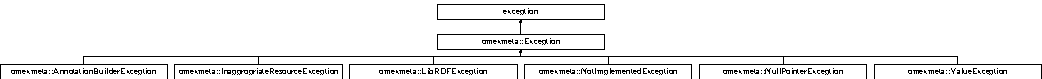
\includegraphics[height=1.056604cm]{classomexmeta_1_1Exception}
\end{center}
\end{figure}
\doxysubsection*{Public Member Functions}
\begin{DoxyCompactItemize}
\item 
\mbox{\hyperlink{classomexmeta_1_1Exception_ad09e2a190a245199974678e2790e81ff}{Exception}} (const char $\ast$message)
\item 
\mbox{\hyperlink{classomexmeta_1_1Exception_ac50b0a25504303cc1a4a1a20de0127eb}{Exception}} (std\+::string message)
\item 
\mbox{\hyperlink{classomexmeta_1_1Exception_aaa08b2467c40a3e28586c0da5da45736}{$\sim$\+Exception}} () noexcept override=default
\item 
const char $\ast$ \mbox{\hyperlink{classomexmeta_1_1Exception_af9c3f258e4715dd2102f5c2db5fbe260}{what}} () const noexcept override
\end{DoxyCompactItemize}
\doxysubsection*{Protected Attributes}
\begin{DoxyCompactItemize}
\item 
std\+::string \mbox{\hyperlink{classomexmeta_1_1Exception_a99067aa4ed7e38cf27b986cca3734512}{msg\+\_\+}}
\end{DoxyCompactItemize}


\doxysubsection{Detailed Description}
\href{https://stackoverflow.com/questions/8152720/correct-way-to-inherit-from-stdexception}{\texttt{ https\+://stackoverflow.\+com/questions/8152720/correct-\/way-\/to-\/inherit-\/from-\/stdexception}} 

\doxysubsection{Constructor \& Destructor Documentation}
\mbox{\Hypertarget{classomexmeta_1_1Exception_ad09e2a190a245199974678e2790e81ff}\label{classomexmeta_1_1Exception_ad09e2a190a245199974678e2790e81ff}} 
\index{omexmeta::Exception@{omexmeta::Exception}!Exception@{Exception}}
\index{Exception@{Exception}!omexmeta::Exception@{omexmeta::Exception}}
\doxysubsubsection{\texorpdfstring{Exception()}{Exception()}\hspace{0.1cm}{\footnotesize\ttfamily [1/2]}}
{\footnotesize\ttfamily omexmeta\+::\+Exception\+::\+Exception (\begin{DoxyParamCaption}\item[{const char $\ast$}]{message }\end{DoxyParamCaption})\hspace{0.3cm}{\ttfamily [inline]}, {\ttfamily [explicit]}}

Constructor (C strings). 
\begin{DoxyParams}{Parameters}
{\em message} & C-\/style string error message. The string contents are copied upon construction. Hence, responsibility for deleting the char$\ast$ lies with the caller. \\
\hline
\end{DoxyParams}
\mbox{\Hypertarget{classomexmeta_1_1Exception_ac50b0a25504303cc1a4a1a20de0127eb}\label{classomexmeta_1_1Exception_ac50b0a25504303cc1a4a1a20de0127eb}} 
\index{omexmeta::Exception@{omexmeta::Exception}!Exception@{Exception}}
\index{Exception@{Exception}!omexmeta::Exception@{omexmeta::Exception}}
\doxysubsubsection{\texorpdfstring{Exception()}{Exception()}\hspace{0.1cm}{\footnotesize\ttfamily [2/2]}}
{\footnotesize\ttfamily omexmeta\+::\+Exception\+::\+Exception (\begin{DoxyParamCaption}\item[{std\+::string}]{message }\end{DoxyParamCaption})\hspace{0.3cm}{\ttfamily [inline]}, {\ttfamily [explicit]}}

Constructor (C++ STL strings). 
\begin{DoxyParams}{Parameters}
{\em message} & The error message. \\
\hline
\end{DoxyParams}
\mbox{\Hypertarget{classomexmeta_1_1Exception_aaa08b2467c40a3e28586c0da5da45736}\label{classomexmeta_1_1Exception_aaa08b2467c40a3e28586c0da5da45736}} 
\index{omexmeta::Exception@{omexmeta::Exception}!````~Exception@{$\sim$Exception}}
\index{````~Exception@{$\sim$Exception}!omexmeta::Exception@{omexmeta::Exception}}
\doxysubsubsection{\texorpdfstring{$\sim$Exception()}{~Exception()}}
{\footnotesize\ttfamily omexmeta\+::\+Exception\+::$\sim$\+Exception (\begin{DoxyParamCaption}{ }\end{DoxyParamCaption})\hspace{0.3cm}{\ttfamily [override]}, {\ttfamily [default]}, {\ttfamily [noexcept]}}

Destructor. Virtual to allow for subclassing. 

\doxysubsection{Member Function Documentation}
\mbox{\Hypertarget{classomexmeta_1_1Exception_af9c3f258e4715dd2102f5c2db5fbe260}\label{classomexmeta_1_1Exception_af9c3f258e4715dd2102f5c2db5fbe260}} 
\index{omexmeta::Exception@{omexmeta::Exception}!what@{what}}
\index{what@{what}!omexmeta::Exception@{omexmeta::Exception}}
\doxysubsubsection{\texorpdfstring{what()}{what()}}
{\footnotesize\ttfamily const char$\ast$ omexmeta\+::\+Exception\+::what (\begin{DoxyParamCaption}{ }\end{DoxyParamCaption}) const\hspace{0.3cm}{\ttfamily [inline]}, {\ttfamily [override]}, {\ttfamily [noexcept]}}

Returns a pointer to the (constant) error description. \begin{DoxyReturn}{Returns}
A pointer to a const char$\ast$. The underlying memory is in posession of the \mbox{\hyperlink{classomexmeta_1_1Exception}{Exception}} object. Callers must not attempt to free the memory. 
\end{DoxyReturn}


\doxysubsection{Member Data Documentation}
\mbox{\Hypertarget{classomexmeta_1_1Exception_a99067aa4ed7e38cf27b986cca3734512}\label{classomexmeta_1_1Exception_a99067aa4ed7e38cf27b986cca3734512}} 
\index{omexmeta::Exception@{omexmeta::Exception}!msg\_@{msg\_}}
\index{msg\_@{msg\_}!omexmeta::Exception@{omexmeta::Exception}}
\doxysubsubsection{\texorpdfstring{msg\_}{msg\_}}
{\footnotesize\ttfamily std\+::string omexmeta\+::\+Exception\+::msg\+\_\+\hspace{0.3cm}{\ttfamily [protected]}}

Error message. 

The documentation for this class was generated from the following file\+:\begin{DoxyCompactItemize}
\item 
src/omexmeta/include/omexmeta/Error.\+h\end{DoxyCompactItemize}

\hypertarget{classException}{}\doxysection{Exception Class Reference}
\label{classException}\index{Exception@{Exception}}
Inheritance diagram for Exception\+:\begin{figure}[H]
\begin{center}
\leavevmode
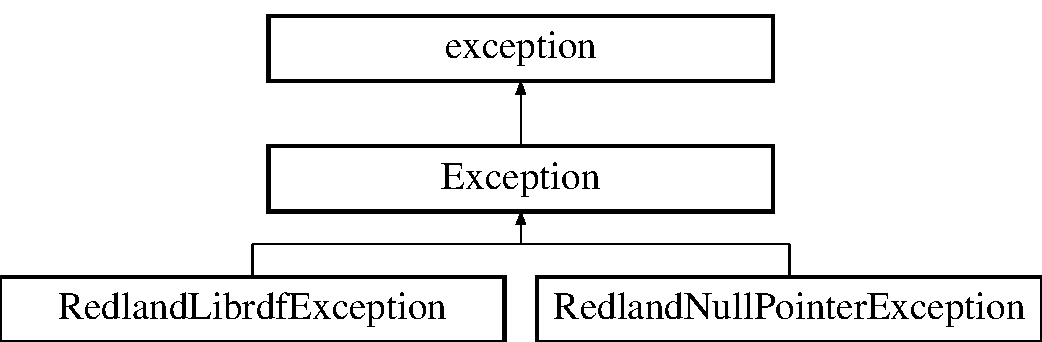
\includegraphics[height=3.000000cm]{classException}
\end{center}
\end{figure}
\doxysubsection*{Public Member Functions}
\begin{DoxyCompactItemize}
\item 
\mbox{\hyperlink{classException_ac541ead5c20548813d7dea73c28c7fab}{Exception}} (const char $\ast$message)
\item 
\mbox{\hyperlink{classException_a0b1693d4d5007815322070c907ee5cc2}{Exception}} (std\+::string message)
\item 
\mbox{\hyperlink{classException_ab834fdbc275748cf287b994503521ada}{$\sim$\+Exception}} () noexcept override=default
\item 
const char $\ast$ \mbox{\hyperlink{classException_ae7ba8334eb35e001b4b0c6df9339c0dc}{what}} () const noexcept override
\end{DoxyCompactItemize}
\doxysubsection*{Protected Attributes}
\begin{DoxyCompactItemize}
\item 
std\+::string \mbox{\hyperlink{classException_a5d59cc46086c61391ed26773ce861780}{msg\+\_\+}}
\end{DoxyCompactItemize}


\doxysubsection{Constructor \& Destructor Documentation}
\mbox{\Hypertarget{classException_ac541ead5c20548813d7dea73c28c7fab}\label{classException_ac541ead5c20548813d7dea73c28c7fab}} 
\index{Exception@{Exception}!Exception@{Exception}}
\index{Exception@{Exception}!Exception@{Exception}}
\doxysubsubsection{\texorpdfstring{Exception()}{Exception()}\hspace{0.1cm}{\footnotesize\ttfamily [1/2]}}
{\footnotesize\ttfamily Exception\+::\+Exception (\begin{DoxyParamCaption}\item[{const char $\ast$}]{message }\end{DoxyParamCaption})\hspace{0.3cm}{\ttfamily [inline]}, {\ttfamily [explicit]}}

Constructor (C strings). 
\begin{DoxyParams}{Parameters}
{\em message} & C-\/style string error message. The string contents are copied upon construction. Hence, responsibility for deleting the char$\ast$ lies with the caller. \\
\hline
\end{DoxyParams}
\mbox{\Hypertarget{classException_a0b1693d4d5007815322070c907ee5cc2}\label{classException_a0b1693d4d5007815322070c907ee5cc2}} 
\index{Exception@{Exception}!Exception@{Exception}}
\index{Exception@{Exception}!Exception@{Exception}}
\doxysubsubsection{\texorpdfstring{Exception()}{Exception()}\hspace{0.1cm}{\footnotesize\ttfamily [2/2]}}
{\footnotesize\ttfamily Exception\+::\+Exception (\begin{DoxyParamCaption}\item[{std\+::string}]{message }\end{DoxyParamCaption})\hspace{0.3cm}{\ttfamily [inline]}, {\ttfamily [explicit]}}

Constructor (C++ STL strings). 
\begin{DoxyParams}{Parameters}
{\em message} & The error message. \\
\hline
\end{DoxyParams}
\mbox{\Hypertarget{classException_ab834fdbc275748cf287b994503521ada}\label{classException_ab834fdbc275748cf287b994503521ada}} 
\index{Exception@{Exception}!````~Exception@{$\sim$Exception}}
\index{````~Exception@{$\sim$Exception}!Exception@{Exception}}
\doxysubsubsection{\texorpdfstring{$\sim$Exception()}{~Exception()}}
{\footnotesize\ttfamily Exception\+::$\sim$\+Exception (\begin{DoxyParamCaption}{ }\end{DoxyParamCaption})\hspace{0.3cm}{\ttfamily [override]}, {\ttfamily [default]}, {\ttfamily [noexcept]}}

Destructor. Virtual to allow for subclassing. 

\doxysubsection{Member Function Documentation}
\mbox{\Hypertarget{classException_ae7ba8334eb35e001b4b0c6df9339c0dc}\label{classException_ae7ba8334eb35e001b4b0c6df9339c0dc}} 
\index{Exception@{Exception}!what@{what}}
\index{what@{what}!Exception@{Exception}}
\doxysubsubsection{\texorpdfstring{what()}{what()}}
{\footnotesize\ttfamily const char$\ast$ Exception\+::what (\begin{DoxyParamCaption}{ }\end{DoxyParamCaption}) const\hspace{0.3cm}{\ttfamily [inline]}, {\ttfamily [override]}, {\ttfamily [noexcept]}}

Returns a pointer to the (constant) error description. \begin{DoxyReturn}{Returns}
A pointer to a const char$\ast$. The underlying memory is in posession of the \mbox{\hyperlink{classException}{Exception}} object. Callers must not attempt to free the memory. 
\end{DoxyReturn}


\doxysubsection{Member Data Documentation}
\mbox{\Hypertarget{classException_a5d59cc46086c61391ed26773ce861780}\label{classException_a5d59cc46086c61391ed26773ce861780}} 
\index{Exception@{Exception}!msg\_@{msg\_}}
\index{msg\_@{msg\_}!Exception@{Exception}}
\doxysubsubsection{\texorpdfstring{msg\_}{msg\_}}
{\footnotesize\ttfamily std\+::string Exception\+::msg\+\_\+\hspace{0.3cm}{\ttfamily [protected]}}

Error message. 

The documentation for this class was generated from the following file\+:\begin{DoxyCompactItemize}
\item 
src/redland/\+Redland\+Wrapper/src/include/redland/Librdf\+Exception.\+h\end{DoxyCompactItemize}

\hypertarget{classomexmeta_1_1Foaf}{}\doxysection{omexmeta\+::Foaf Class Reference}
\label{classomexmeta_1_1Foaf}\index{omexmeta::Foaf@{omexmeta::Foaf}}
Inheritance diagram for omexmeta\+::Foaf\+:\begin{figure}[H]
\begin{center}
\leavevmode
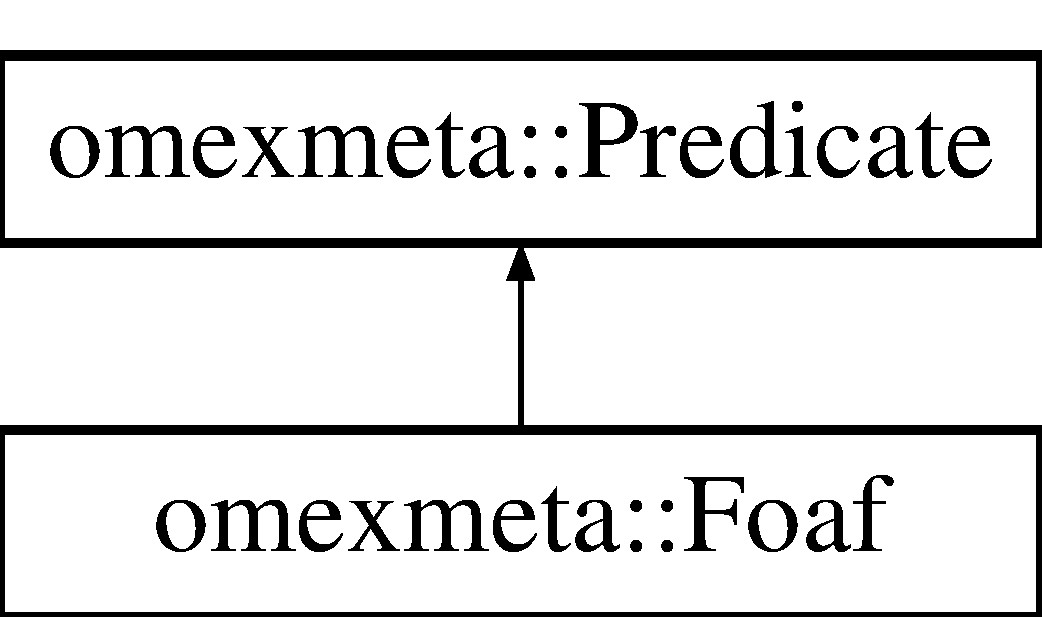
\includegraphics[height=2.000000cm]{classomexmeta_1_1Foaf}
\end{center}
\end{figure}
\doxysubsection*{Public Member Functions}
\begin{DoxyCompactItemize}
\item 
\mbox{\Hypertarget{classomexmeta_1_1Foaf_af60965a79363573d9df78010936e1c81}\label{classomexmeta_1_1Foaf_af60965a79363573d9df78010936e1c81}} 
{\bfseries Foaf} (const std\+::string \&term)
\item 
\mbox{\Hypertarget{classomexmeta_1_1Foaf_a044d1eedbaf2be1ac6fcd160e3365a16}\label{classomexmeta_1_1Foaf_a044d1eedbaf2be1ac6fcd160e3365a16}} 
void {\bfseries verify} ()
\end{DoxyCompactItemize}
\doxysubsection*{Public Attributes}
\begin{DoxyCompactItemize}
\item 
std\+::vector$<$ std\+::string $>$ {\bfseries valid\+\_\+terms\+\_\+}
\end{DoxyCompactItemize}
\doxysubsection*{Additional Inherited Members}


\doxysubsection{Member Data Documentation}
\mbox{\Hypertarget{classomexmeta_1_1Foaf_a5a91260f5319adc671c749a09ef0cf0a}\label{classomexmeta_1_1Foaf_a5a91260f5319adc671c749a09ef0cf0a}} 
\index{omexmeta::Foaf@{omexmeta::Foaf}!valid\_terms\_@{valid\_terms\_}}
\index{valid\_terms\_@{valid\_terms\_}!omexmeta::Foaf@{omexmeta::Foaf}}
\doxysubsubsection{\texorpdfstring{valid\_terms\_}{valid\_terms\_}}
{\footnotesize\ttfamily std\+::vector$<$std\+::string$>$ omexmeta\+::\+Foaf\+::valid\+\_\+terms\+\_\+}

{\bfseries Initial value\+:}
\begin{DoxyCode}{0}
\DoxyCodeLine{\{}
\DoxyCodeLine{                \textcolor{stringliteral}{"{}Agent"{}}, \textcolor{stringliteral}{"{}Person"{}}, \textcolor{stringliteral}{"{}name"{}}, \textcolor{stringliteral}{"{}title"{}}, \textcolor{stringliteral}{"{}img"{}}, \textcolor{stringliteral}{"{}depiction"{}}, \textcolor{stringliteral}{"{}familyName"{}}, \textcolor{stringliteral}{"{}givenName"{}}, \textcolor{stringliteral}{"{}knows"{}},}
\DoxyCodeLine{                \textcolor{stringliteral}{"{}based\_near"{}}, \textcolor{stringliteral}{"{}age"{}}, \textcolor{stringliteral}{"{}made"{}}, \textcolor{stringliteral}{"{}primaryTopic"{}}, \textcolor{stringliteral}{"{}Project"{}}, \textcolor{stringliteral}{"{}Organization"{}}, \textcolor{stringliteral}{"{}Group"{}}, \textcolor{stringliteral}{"{}member"{}},}
\DoxyCodeLine{                \textcolor{stringliteral}{"{}Document"{}}, \textcolor{stringliteral}{"{}Image"{}}, \textcolor{stringliteral}{"{}nick"{}}, \textcolor{stringliteral}{"{}mbox"{}}, \textcolor{stringliteral}{"{}homepage"{}}, \textcolor{stringliteral}{"{}weblog"{}}, \textcolor{stringliteral}{"{}openid"{}}, \textcolor{stringliteral}{"{}jabberID"{}}, \textcolor{stringliteral}{"{}mbox\_sha1sum"{}},}
\DoxyCodeLine{                \textcolor{stringliteral}{"{}interest"{}}, \textcolor{stringliteral}{"{}topic\_interest"{}}, \textcolor{stringliteral}{"{}topic"{}}, \textcolor{stringliteral}{"{}workplaceHomepage"{}}, \textcolor{stringliteral}{"{}workInfoHomepage"{}}, \textcolor{stringliteral}{"{}schoolHomepage"{}},}
\DoxyCodeLine{                \textcolor{stringliteral}{"{}publications"{}}, \textcolor{stringliteral}{"{}currentProject"{}}, \textcolor{stringliteral}{"{}pastProject"{}}, \textcolor{stringliteral}{"{}account"{}}, \textcolor{stringliteral}{"{}OnlineAccount"{}}, \textcolor{stringliteral}{"{}accountName"{}},}
\DoxyCodeLine{                \textcolor{stringliteral}{"{}accountServiceHomepage"{}}, \textcolor{stringliteral}{"{}PersonalProfileDocument"{}}, \textcolor{stringliteral}{"{}tipjar"{}}, \textcolor{stringliteral}{"{}sha1"{}}, \textcolor{stringliteral}{"{}thumbnail"{}}, \textcolor{stringliteral}{"{}logo"{}},\}}

\end{DoxyCode}


The documentation for this class was generated from the following files\+:\begin{DoxyCompactItemize}
\item 
src/omexmeta/Predicate.\+h\item 
src/omexmeta/Predicate.\+cpp\end{DoxyCompactItemize}

\hypertarget{structdbg_1_1detail_1_1has__ostream__operator}{}\doxysection{dbg\+::detail\+::has\+\_\+ostream\+\_\+operator$<$ T $>$ Struct Template Reference}
\label{structdbg_1_1detail_1_1has__ostream__operator}\index{dbg::detail::has\_ostream\_operator$<$ T $>$@{dbg::detail::has\_ostream\_operator$<$ T $>$}}
Inheritance diagram for dbg\+::detail\+::has\+\_\+ostream\+\_\+operator$<$ T $>$\+:\begin{figure}[H]
\begin{center}
\leavevmode
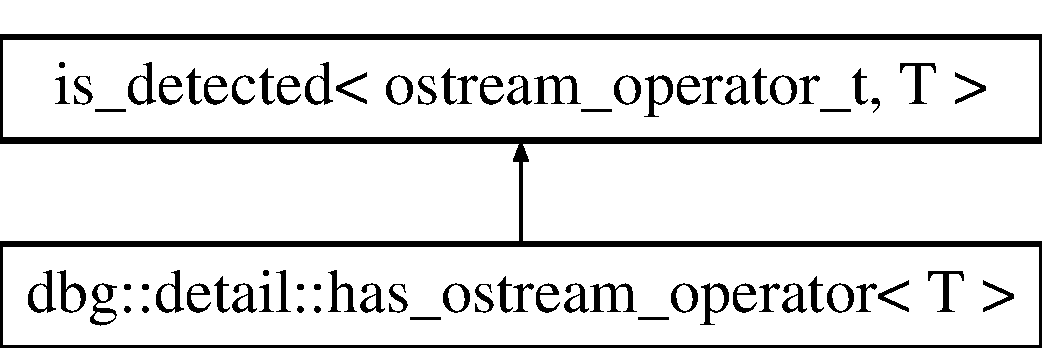
\includegraphics[height=2.000000cm]{structdbg_1_1detail_1_1has__ostream__operator}
\end{center}
\end{figure}


The documentation for this struct was generated from the following file\+:\begin{DoxyCompactItemize}
\item 
src/omexmeta/include/omexmeta/dbg.\+h\end{DoxyCompactItemize}

\hypertarget{classomexmeta_1_1InappropriateResourceException}{}\section{omexmeta\+:\+:Inappropriate\+Resource\+Exception Class Reference}
\label{classomexmeta_1_1InappropriateResourceException}\index{omexmeta\+::\+Inappropriate\+Resource\+Exception@{omexmeta\+::\+Inappropriate\+Resource\+Exception}}
Inheritance diagram for omexmeta\+:\+:Inappropriate\+Resource\+Exception\+:\begin{figure}[H]
\begin{center}
\leavevmode
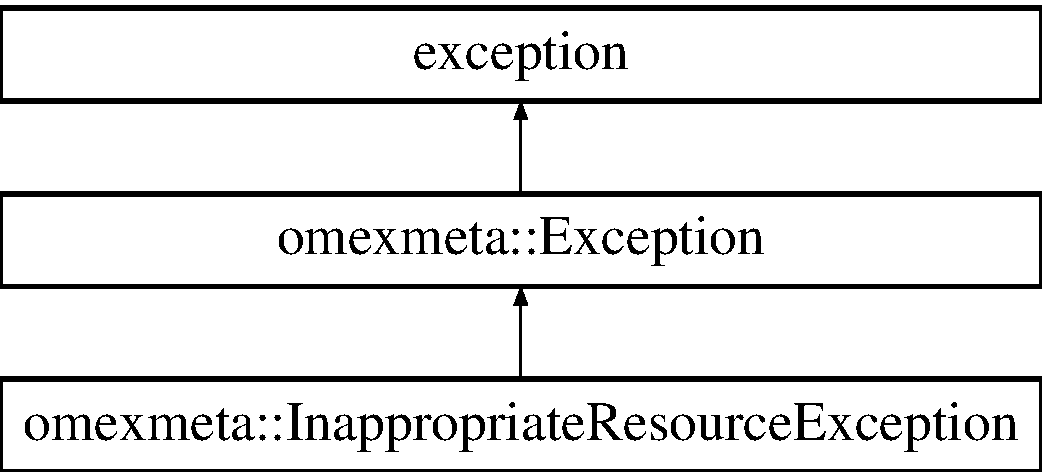
\includegraphics[height=3.000000cm]{classomexmeta_1_1InappropriateResourceException}
\end{center}
\end{figure}
\subsection*{Additional Inherited Members}


The documentation for this class was generated from the following file\+:\begin{DoxyCompactItemize}
\item 
src/omexmeta/Error.\+h\end{DoxyCompactItemize}

\hypertarget{structdbg_1_1detail_1_1is__container}{}\doxysection{dbg\+::detail\+::is\+\_\+container$<$ T $>$ Struct Template Reference}
\label{structdbg_1_1detail_1_1is__container}\index{dbg::detail::is\_container$<$ T $>$@{dbg::detail::is\_container$<$ T $>$}}
\doxysubsection*{Static Public Attributes}
\begin{DoxyCompactItemize}
\item 
static constexpr bool {\bfseries value}
\end{DoxyCompactItemize}


\doxysubsection{Member Data Documentation}
\mbox{\Hypertarget{structdbg_1_1detail_1_1is__container_aa9a4594488352384b65b36198ac414f8}\label{structdbg_1_1detail_1_1is__container_aa9a4594488352384b65b36198ac414f8}} 
\index{dbg::detail::is\_container$<$ T $>$@{dbg::detail::is\_container$<$ T $>$}!value@{value}}
\index{value@{value}!dbg::detail::is\_container$<$ T $>$@{dbg::detail::is\_container$<$ T $>$}}
\doxysubsubsection{\texorpdfstring{value}{value}}
{\footnotesize\ttfamily template$<$typename T $>$ \\
constexpr bool \mbox{\hyperlink{structdbg_1_1detail_1_1is__container}{dbg\+::detail\+::is\+\_\+container}}$<$ T $>$\+::value\hspace{0.3cm}{\ttfamily [static]}, {\ttfamily [constexpr]}}

{\bfseries Initial value\+:}
\begin{DoxyCode}{0}
\DoxyCodeLine{=}
\DoxyCodeLine{      is\_detected<detect\_begin\_t, T>::value \&\&}
\DoxyCodeLine{      is\_detected<detect\_end\_t, T>::value \&\&}
\DoxyCodeLine{      is\_detected<detect\_size\_t, T>::value \&\&}
\DoxyCodeLine{      !std::is\_same<std::string,}
\DoxyCodeLine{                    \textcolor{keyword}{typename} std::remove\_cv<}
\DoxyCodeLine{                        \textcolor{keyword}{typename} std::remove\_reference<T>::type>::type>::value}

\end{DoxyCode}


The documentation for this struct was generated from the following file\+:\begin{DoxyCompactItemize}
\item 
src/omexmeta/include/omexmeta/dbg.\+h\end{DoxyCompactItemize}

\hypertarget{structdbg_1_1last}{}\doxysection{dbg\+::last$<$ T, U $>$ Struct Template Reference}
\label{structdbg_1_1last}\index{dbg::last$<$ T, U $>$@{dbg::last$<$ T, U $>$}}
\doxysubsection*{Public Types}
\begin{DoxyCompactItemize}
\item 
\mbox{\Hypertarget{structdbg_1_1last_aac2d6dd66fecfc0f3f37ecb4a02b0779}\label{structdbg_1_1last_aac2d6dd66fecfc0f3f37ecb4a02b0779}} 
using {\bfseries type} = typename \mbox{\hyperlink{structdbg_1_1last}{last}}$<$ U... $>$\+::type
\end{DoxyCompactItemize}


The documentation for this struct was generated from the following file\+:\begin{DoxyCompactItemize}
\item 
src/omexmeta/dbg.\+h\end{DoxyCompactItemize}

\hypertarget{structdbg_1_1last_3_01T_01_4}{}\doxysection{dbg\+::last$<$ T $>$ Struct Template Reference}
\label{structdbg_1_1last_3_01T_01_4}\index{dbg::last$<$ T $>$@{dbg::last$<$ T $>$}}
\doxysubsection*{Public Types}
\begin{DoxyCompactItemize}
\item 
\mbox{\Hypertarget{structdbg_1_1last_3_01T_01_4_a6715c2f60dfaa8a096517ce45ff43999}\label{structdbg_1_1last_3_01T_01_4_a6715c2f60dfaa8a096517ce45ff43999}} 
using {\bfseries type} = T
\end{DoxyCompactItemize}


The documentation for this struct was generated from the following file\+:\begin{DoxyCompactItemize}
\item 
src/omexmeta/include/omexmeta/dbg.\+h\end{DoxyCompactItemize}

\hypertarget{classomexmeta_1_1LibRDFException}{}\doxysection{omexmeta\+::Lib\+R\+D\+F\+Exception Class Reference}
\label{classomexmeta_1_1LibRDFException}\index{omexmeta::LibRDFException@{omexmeta::LibRDFException}}
Inheritance diagram for omexmeta\+::Lib\+R\+D\+F\+Exception\+:\begin{figure}[H]
\begin{center}
\leavevmode
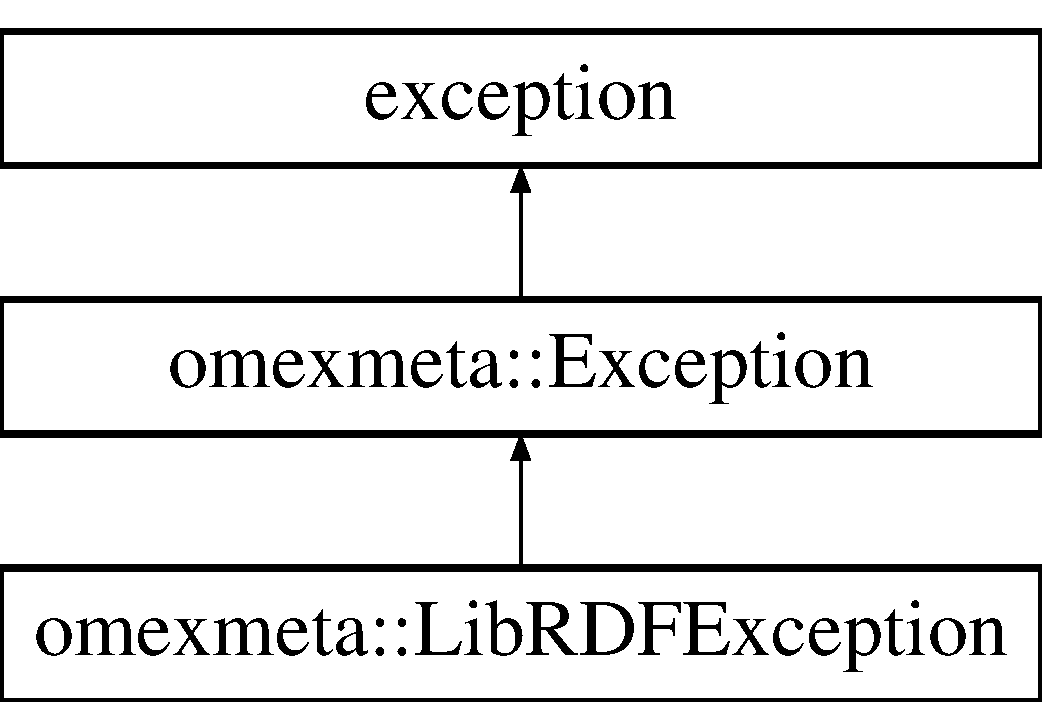
\includegraphics[height=3.000000cm]{classomexmeta_1_1LibRDFException}
\end{center}
\end{figure}
\doxysubsection*{Additional Inherited Members}


The documentation for this class was generated from the following file\+:\begin{DoxyCompactItemize}
\item 
src/omexmeta/include/omexmeta/Error.\+h\end{DoxyCompactItemize}

\hypertarget{classredland_1_1LibrdfModel}{}\section{redland\+:\+:Librdf\+Model Class Reference}
\label{classredland_1_1LibrdfModel}\index{redland\+::\+Librdf\+Model@{redland\+::\+Librdf\+Model}}
\subsection*{Public Member Functions}
\begin{DoxyCompactItemize}
\item 
\mbox{\Hypertarget{classredland_1_1LibrdfModel_a5a35c032585e38b1d41bc18f057128c1}\label{classredland_1_1LibrdfModel_a5a35c032585e38b1d41bc18f057128c1}} 
{\bfseries Librdf\+Model} (const \hyperlink{classredland_1_1LibrdfModel}{Librdf\+Model} \&model)=delete
\item 
\mbox{\Hypertarget{classredland_1_1LibrdfModel_a583e0eaecfe167ccbbeac5d768bcd644}\label{classredland_1_1LibrdfModel_a583e0eaecfe167ccbbeac5d768bcd644}} 
{\bfseries Librdf\+Model} (\hyperlink{classredland_1_1LibrdfModel}{Librdf\+Model} \&\&model) noexcept
\item 
\mbox{\Hypertarget{classredland_1_1LibrdfModel_a7bd07324b31fa8eb8f5f2e51b15044fc}\label{classredland_1_1LibrdfModel_a7bd07324b31fa8eb8f5f2e51b15044fc}} 
\hyperlink{classredland_1_1LibrdfModel}{Librdf\+Model} \& {\bfseries operator=} (const \hyperlink{classredland_1_1LibrdfModel}{Librdf\+Model} \&model)=delete
\item 
\mbox{\Hypertarget{classredland_1_1LibrdfModel_a9007acfb92943e018d20d6985c811033}\label{classredland_1_1LibrdfModel_a9007acfb92943e018d20d6985c811033}} 
\hyperlink{classredland_1_1LibrdfModel}{Librdf\+Model} \& {\bfseries operator=} (\hyperlink{classredland_1_1LibrdfModel}{Librdf\+Model} \&\&model) noexcept
\item 
\mbox{\Hypertarget{classredland_1_1LibrdfModel_a8b7d3063e030ce8613dcd6def7463a5a}\label{classredland_1_1LibrdfModel_a8b7d3063e030ce8613dcd6def7463a5a}} 
{\bfseries Librdf\+Model} (librdf\+\_\+model $\ast$model)
\item 
\mbox{\Hypertarget{classredland_1_1LibrdfModel_a355e16664fa50a8a3085f4070347106f}\label{classredland_1_1LibrdfModel_a355e16664fa50a8a3085f4070347106f}} 
{\bfseries Librdf\+Model} (librdf\+\_\+storage $\ast$storage, const char $\ast$options=nullptr)
\item 
\mbox{\Hypertarget{classredland_1_1LibrdfModel_ae1b996f1785adfe9b4a1824a73643248}\label{classredland_1_1LibrdfModel_ae1b996f1785adfe9b4a1824a73643248}} 
librdf\+\_\+model $\ast$ {\bfseries get} () const
\item 
\mbox{\Hypertarget{classredland_1_1LibrdfModel_a29e79bafe40a64141ab7edf8ecbbbdd3}\label{classredland_1_1LibrdfModel_a29e79bafe40a64141ab7edf8ecbbbdd3}} 
\hyperlink{classredland_1_1LibrdfQueryResults}{Librdf\+Query\+Results} {\bfseries query} (\hyperlink{classredland_1_1LibrdfQuery}{Librdf\+Query} query)
\item 
\mbox{\Hypertarget{classredland_1_1LibrdfModel_a646ed92896c4030de31c9e17b881bd2a}\label{classredland_1_1LibrdfModel_a646ed92896c4030de31c9e17b881bd2a}} 
\hyperlink{classredland_1_1LibrdfStream}{Librdf\+Stream} {\bfseries to\+Stream} ()
\item 
\mbox{\Hypertarget{classredland_1_1LibrdfModel_a3067eb5bae1353ab5c86f135c4b401ad}\label{classredland_1_1LibrdfModel_a3067eb5bae1353ab5c86f135c4b401ad}} 
int {\bfseries size} () const
\item 
\mbox{\Hypertarget{classredland_1_1LibrdfModel_a2b565a7d705e24d6163c068a40040087}\label{classredland_1_1LibrdfModel_a2b565a7d705e24d6163c068a40040087}} 
void {\bfseries add\+Statement} (const \hyperlink{classredland_1_1LibrdfStatement}{Librdf\+Statement} \&statement) const
\item 
\mbox{\Hypertarget{classredland_1_1LibrdfModel_a643c3e3d3363f4f06330ede73dc19514}\label{classredland_1_1LibrdfModel_a643c3e3d3363f4f06330ede73dc19514}} 
void {\bfseries add\+Statement} (librdf\+\_\+statement $\ast$statement) const
\item 
\mbox{\Hypertarget{classredland_1_1LibrdfModel_ad145b8f46be49434bb8bd0b90a904770}\label{classredland_1_1LibrdfModel_ad145b8f46be49434bb8bd0b90a904770}} 
void {\bfseries free\+Model} ()
\end{DoxyCompactItemize}


The documentation for this class was generated from the following files\+:\begin{DoxyCompactItemize}
\item 
src/redland/\+Redland\+A\+P\+I\+Wrapper/src/Librdf\+Model.\+h\item 
src/redland/\+Redland\+A\+P\+I\+Wrapper/src/Librdf\+Model.\+cpp\end{DoxyCompactItemize}

\hypertarget{classredland_1_1LibrdfNode}{}\doxysection{redland\+::Librdf\+Node Class Reference}
\label{classredland_1_1LibrdfNode}\index{redland::LibrdfNode@{redland::LibrdfNode}}
\doxysubsection*{Public Member Functions}
\begin{DoxyCompactItemize}
\item 
\mbox{\Hypertarget{classredland_1_1LibrdfNode_afc1bdf57705253e8204a394541b96ca7}\label{classredland_1_1LibrdfNode_afc1bdf57705253e8204a394541b96ca7}} 
bool {\bfseries operator==} (const \mbox{\hyperlink{classredland_1_1LibrdfNode}{Librdf\+Node}} \&rhs) const
\item 
\mbox{\Hypertarget{classredland_1_1LibrdfNode_aefbf9e2bf34eb0171932e39323eadfd8}\label{classredland_1_1LibrdfNode_aefbf9e2bf34eb0171932e39323eadfd8}} 
bool {\bfseries operator!=} (const \mbox{\hyperlink{classredland_1_1LibrdfNode}{Librdf\+Node}} \&rhs) const
\item 
\mbox{\Hypertarget{classredland_1_1LibrdfNode_a28f6ce060bddf7e1cb88d17d4d4ea81a}\label{classredland_1_1LibrdfNode_a28f6ce060bddf7e1cb88d17d4d4ea81a}} 
void {\bfseries free\+Node} ()
\item 
\mbox{\Hypertarget{classredland_1_1LibrdfNode_a669557dc1240dc17c3a7a3a61d2400d9}\label{classredland_1_1LibrdfNode_a669557dc1240dc17c3a7a3a61d2400d9}} 
{\bfseries Librdf\+Node} (const \mbox{\hyperlink{classredland_1_1LibrdfNode}{Librdf\+Node}} \&node)=delete
\item 
\mbox{\Hypertarget{classredland_1_1LibrdfNode_a822ce6a4221315abe5768b278b83d0e5}\label{classredland_1_1LibrdfNode_a822ce6a4221315abe5768b278b83d0e5}} 
{\bfseries Librdf\+Node} (\mbox{\hyperlink{classredland_1_1LibrdfNode}{Librdf\+Node}} \&\&node) noexcept
\item 
\mbox{\Hypertarget{classredland_1_1LibrdfNode_abce52c34cc89e48886cde07aa5e113c9}\label{classredland_1_1LibrdfNode_abce52c34cc89e48886cde07aa5e113c9}} 
\mbox{\hyperlink{classredland_1_1LibrdfNode}{Librdf\+Node}} \& {\bfseries operator=} (const \mbox{\hyperlink{classredland_1_1LibrdfNode}{Librdf\+Node}} \&node)=delete
\item 
\mbox{\Hypertarget{classredland_1_1LibrdfNode_a9de3a69b00958b2bb50646dbf0aa8d7e}\label{classredland_1_1LibrdfNode_a9de3a69b00958b2bb50646dbf0aa8d7e}} 
\mbox{\hyperlink{classredland_1_1LibrdfNode}{Librdf\+Node}} \& {\bfseries operator=} (\mbox{\hyperlink{classredland_1_1LibrdfNode}{Librdf\+Node}} \&\&node) noexcept
\item 
\mbox{\Hypertarget{classredland_1_1LibrdfNode_a200c7a67088e66d6fc73f52bdb51d2e9}\label{classredland_1_1LibrdfNode_a200c7a67088e66d6fc73f52bdb51d2e9}} 
{\bfseries Librdf\+Node} (librdf\+\_\+node $\ast$node)
\item 
\mbox{\Hypertarget{classredland_1_1LibrdfNode_a33162ea36efe451c100325816cf8613f}\label{classredland_1_1LibrdfNode_a33162ea36efe451c100325816cf8613f}} 
librdf\+\_\+node $\ast$ {\bfseries get} () const
\item 
\mbox{\Hypertarget{classredland_1_1LibrdfNode_a83ec604f27e71cea80ac49569a06ddfe}\label{classredland_1_1LibrdfNode_a83ec604f27e71cea80ac49569a06ddfe}} 
raptor\+\_\+term\+\_\+type {\bfseries get\+Raptor\+Term\+Type} ()
\item 
\mbox{\Hypertarget{classredland_1_1LibrdfNode_a535fbe1bc21ca9cd9b39b969bfd2e500}\label{classredland_1_1LibrdfNode_a535fbe1bc21ca9cd9b39b969bfd2e500}} 
std\+::string {\bfseries str} () const
\item 
\mbox{\Hypertarget{classredland_1_1LibrdfNode_a98487d5af58971d820fcb99c88d8712d}\label{classredland_1_1LibrdfNode_a98487d5af58971d820fcb99c88d8712d}} 
\mbox{\hyperlink{classredland_1_1LibrdfUri}{Librdf\+Uri}} {\bfseries get\+Literal\+Datatype} ()
\item 
\mbox{\Hypertarget{classredland_1_1LibrdfNode_a58b9962c783be77fd0d2cb7036bfdc6a}\label{classredland_1_1LibrdfNode_a58b9962c783be77fd0d2cb7036bfdc6a}} 
std\+::string {\bfseries get\+Literal\+Language} ()
\item 
\mbox{\Hypertarget{classredland_1_1LibrdfNode_a49431de8c3262ee56d533a5fe047ee00}\label{classredland_1_1LibrdfNode_a49431de8c3262ee56d533a5fe047ee00}} 
std\+::string {\bfseries get\+Blank\+Identifier} ()
\item 
\mbox{\Hypertarget{classredland_1_1LibrdfNode_a0dd2ff697c0753eddf7327f64390ed77}\label{classredland_1_1LibrdfNode_a0dd2ff697c0753eddf7327f64390ed77}} 
\mbox{\hyperlink{classredland_1_1LibrdfUri}{Librdf\+Uri}} {\bfseries get\+Uri} ()
\item 
\mbox{\Hypertarget{classredland_1_1LibrdfNode_a01aeb7675187379674746f803a1fbdc9}\label{classredland_1_1LibrdfNode_a01aeb7675187379674746f803a1fbdc9}} 
void {\bfseries set\+Uri} (const std\+::string \&uri)
\item 
\mbox{\Hypertarget{classredland_1_1LibrdfNode_a160db9f7c7636c339e12c26f519b8fff}\label{classredland_1_1LibrdfNode_a160db9f7c7636c339e12c26f519b8fff}} 
void {\bfseries set\+Literal\+Datatype} (const std\+::string \&datatype)
\item 
\mbox{\Hypertarget{classredland_1_1LibrdfNode_afd81499fe4125cc2f4c472d33fb6c8c0}\label{classredland_1_1LibrdfNode_afd81499fe4125cc2f4c472d33fb6c8c0}} 
void {\bfseries set\+Blank\+Identifier} (const std\+::string \&identifier)
\item 
\mbox{\Hypertarget{classredland_1_1LibrdfNode_a8ac1d280707f4405dc8865465028ae33}\label{classredland_1_1LibrdfNode_a8ac1d280707f4405dc8865465028ae33}} 
\mbox{\hyperlink{classredland_1_1LibrdfNode}{Librdf\+Node}} {\bfseries from\+Uri\+String} (const std\+::string \&uri\+\_\+string, const std\+::string \&local\+\_\+prefix)
\end{DoxyCompactItemize}
\doxysubsection*{Static Public Member Functions}
\begin{DoxyCompactItemize}
\item 
\mbox{\Hypertarget{classredland_1_1LibrdfNode_a5c971e6daeca94c4eabddfa5f6e4c456}\label{classredland_1_1LibrdfNode_a5c971e6daeca94c4eabddfa5f6e4c456}} 
static void {\bfseries free\+Node} (librdf\+\_\+node $\ast$node)
\item 
\mbox{\Hypertarget{classredland_1_1LibrdfNode_aacf853ee60f9d706bc7e95fb426166bd}\label{classredland_1_1LibrdfNode_aacf853ee60f9d706bc7e95fb426166bd}} 
static \mbox{\hyperlink{classredland_1_1LibrdfNode}{Librdf\+Node}} {\bfseries from\+Uri\+String} (const std\+::string \&uri\+\_\+string)
\item 
\mbox{\Hypertarget{classredland_1_1LibrdfNode_a22ea96262be432e6abb5c1e28ede3071}\label{classredland_1_1LibrdfNode_a22ea96262be432e6abb5c1e28ede3071}} 
static \mbox{\hyperlink{classredland_1_1LibrdfNode}{Librdf\+Node}} {\bfseries from\+Blank} (const std\+::string \&blank)
\item 
\mbox{\Hypertarget{classredland_1_1LibrdfNode_a346fad618a010ef983ce24d62891de0e}\label{classredland_1_1LibrdfNode_a346fad618a010ef983ce24d62891de0e}} 
static \mbox{\hyperlink{classredland_1_1LibrdfNode}{Librdf\+Node}} {\bfseries from\+Literal} (const std\+::string \&literal, const std\+::string \&literal\+\_\+datatype\+\_\+uri=\char`\"{}string\char`\"{}, const std\+::string \&xml\+\_\+language=std\+::string())
\item 
\mbox{\Hypertarget{classredland_1_1LibrdfNode_aaeeeca26bafdaf7f118af3307a4768be}\label{classredland_1_1LibrdfNode_aaeeeca26bafdaf7f118af3307a4768be}} 
static \mbox{\hyperlink{classredland_1_1LibrdfNode}{Librdf\+Node}} {\bfseries new\+Empty\+Node} ()
\item 
\mbox{\Hypertarget{classredland_1_1LibrdfNode_aa6bf7e25e68e473f2f39cb7b4cb5f39b}\label{classredland_1_1LibrdfNode_aa6bf7e25e68e473f2f39cb7b4cb5f39b}} 
static std\+::string {\bfseries str} (librdf\+\_\+node $\ast$node)
\item 
\mbox{\Hypertarget{classredland_1_1LibrdfNode_a3242e29edb736ba0aa8ac42fd6b3ae58}\label{classredland_1_1LibrdfNode_a3242e29edb736ba0aa8ac42fd6b3ae58}} 
static std\+::string {\bfseries validate\+Literal\+Datatype} (const std\+::string \&literal\+\_\+datatype\+\_\+uri)
\item 
\mbox{\Hypertarget{classredland_1_1LibrdfNode_a46208d163a49bc7640a8b4c847e2a28b}\label{classredland_1_1LibrdfNode_a46208d163a49bc7640a8b4c847e2a28b}} 
static \mbox{\hyperlink{classredland_1_1LibrdfNode}{Librdf\+Node}} {\bfseries copy\+Node} (const \mbox{\hyperlink{classredland_1_1LibrdfNode}{Librdf\+Node}} \&node)
\item 
\mbox{\Hypertarget{classredland_1_1LibrdfNode_a872032a7516dd140f93a9f4af3e0abd9}\label{classredland_1_1LibrdfNode_a872032a7516dd140f93a9f4af3e0abd9}} 
static \mbox{\hyperlink{classredland_1_1LibrdfNode}{Librdf\+Node}} {\bfseries from\+Relative\+Uri} (const std\+::string \&uri\+\_\+string, const std\+::string \&base\+\_\+uri)
\end{DoxyCompactItemize}


The documentation for this class was generated from the following files\+:\begin{DoxyCompactItemize}
\item 
src/redland/\+Redland\+Wrapper/src/Librdf\+Node.\+h\item 
src/redland/\+Redland\+Wrapper/src/Librdf\+Node.\+cpp\end{DoxyCompactItemize}

\hypertarget{classredland_1_1LibrdfParser}{}\doxysection{redland\+::Librdf\+Parser Class Reference}
\label{classredland_1_1LibrdfParser}\index{redland::LibrdfParser@{redland::LibrdfParser}}
\doxysubsection*{Public Member Functions}
\begin{DoxyCompactItemize}
\item 
\mbox{\Hypertarget{classredland_1_1LibrdfParser_a884b4e7cb05942390fba7765cfb3aec8}\label{classredland_1_1LibrdfParser_a884b4e7cb05942390fba7765cfb3aec8}} 
{\bfseries Librdf\+Parser} (const \mbox{\hyperlink{classredland_1_1LibrdfParser}{Librdf\+Parser}} \&parser)=delete
\item 
\mbox{\Hypertarget{classredland_1_1LibrdfParser_a8c75ee321bd82076491aa0d63d0664c8}\label{classredland_1_1LibrdfParser_a8c75ee321bd82076491aa0d63d0664c8}} 
{\bfseries Librdf\+Parser} (\mbox{\hyperlink{classredland_1_1LibrdfParser}{Librdf\+Parser}} \&\&parser) noexcept
\item 
\mbox{\Hypertarget{classredland_1_1LibrdfParser_aeee1312383f2e3f72e49076390a2a27b}\label{classredland_1_1LibrdfParser_aeee1312383f2e3f72e49076390a2a27b}} 
\mbox{\hyperlink{classredland_1_1LibrdfParser}{Librdf\+Parser}} \& {\bfseries operator=} (const \mbox{\hyperlink{classredland_1_1LibrdfParser}{Librdf\+Parser}} \&parser)=delete
\item 
\mbox{\Hypertarget{classredland_1_1LibrdfParser_a5a5e09075b43906c9161d453ac63ab8a}\label{classredland_1_1LibrdfParser_a5a5e09075b43906c9161d453ac63ab8a}} 
\mbox{\hyperlink{classredland_1_1LibrdfParser}{Librdf\+Parser}} \& {\bfseries operator=} (\mbox{\hyperlink{classredland_1_1LibrdfParser}{Librdf\+Parser}} \&\&parser) noexcept
\item 
\mbox{\Hypertarget{classredland_1_1LibrdfParser_ac1373b22444c108a2a67dbf24fa4ca92}\label{classredland_1_1LibrdfParser_ac1373b22444c108a2a67dbf24fa4ca92}} 
{\bfseries Librdf\+Parser} (librdf\+\_\+parser $\ast$parser)
\item 
\mbox{\Hypertarget{classredland_1_1LibrdfParser_ac594c85ec97a39cad1aa557c98c39eb1}\label{classredland_1_1LibrdfParser_ac594c85ec97a39cad1aa557c98c39eb1}} 
{\bfseries Librdf\+Parser} (std\+::string format, std\+::string mime\+\_\+type=std\+::string(), const std\+::string \&type\+\_\+uri=std\+::string())
\item 
\mbox{\Hypertarget{classredland_1_1LibrdfParser_aadb297b986879ca618d3092fe737d41c}\label{classredland_1_1LibrdfParser_aadb297b986879ca618d3092fe737d41c}} 
librdf\+\_\+parser $\ast$ {\bfseries get} () const
\item 
\mbox{\Hypertarget{classredland_1_1LibrdfParser_a1e2098e2c99ba886ab1521048258600c}\label{classredland_1_1LibrdfParser_a1e2098e2c99ba886ab1521048258600c}} 
int {\bfseries num\+Namespaces\+Seen} () const
\item 
\mbox{\Hypertarget{classredland_1_1LibrdfParser_aed92021f88bccfa26bf78c29797b4208}\label{classredland_1_1LibrdfParser_aed92021f88bccfa26bf78c29797b4208}} 
std\+::string {\bfseries get\+Namespaces\+Seen\+Uri} (int index) const
\item 
\mbox{\Hypertarget{classredland_1_1LibrdfParser_a86739506ba32a9a6da8b69711f1026db}\label{classredland_1_1LibrdfParser_a86739506ba32a9a6da8b69711f1026db}} 
void {\bfseries parse\+String} (const std\+::string \&rdf\+\_\+string, const \mbox{\hyperlink{classredland_1_1LibrdfModel}{Librdf\+Model}} \&model, const \mbox{\hyperlink{classredland_1_1LibrdfUri}{Librdf\+Uri}} \&base\+\_\+uri) const
\item 
\mbox{\Hypertarget{classredland_1_1LibrdfParser_a2a7ac5ac97b4bc5876db02f0b9c7b987}\label{classredland_1_1LibrdfParser_a2a7ac5ac97b4bc5876db02f0b9c7b987}} 
void {\bfseries parse\+String} (const std\+::string \&rdf\+\_\+string, const \mbox{\hyperlink{classredland_1_1LibrdfModel}{Librdf\+Model}} \&model, const std\+::string \&base\+\_\+uri) const
\item 
\mbox{\Hypertarget{classredland_1_1LibrdfParser_a14c24e47699166e3b5bd4141ebd946ff}\label{classredland_1_1LibrdfParser_a14c24e47699166e3b5bd4141ebd946ff}} 
void {\bfseries parse\+File} (const std\+::string \&filename\+\_\+uri, const \mbox{\hyperlink{classredland_1_1LibrdfModel}{Librdf\+Model}} \&model, const std\+::string \&local\+\_\+uri) const
\item 
\mbox{\Hypertarget{classredland_1_1LibrdfParser_a15ffb21bf48e486708eab820719827a6}\label{classredland_1_1LibrdfParser_a15ffb21bf48e486708eab820719827a6}} 
void {\bfseries parse\+File} (const std\+::string \&filename\+\_\+uri, const \mbox{\hyperlink{classredland_1_1LibrdfModel}{Librdf\+Model}} \&model) const
\item 
\mbox{\Hypertarget{classredland_1_1LibrdfParser_a733bf5d33a2d71bd6d7c201e1c952b04}\label{classredland_1_1LibrdfParser_a733bf5d33a2d71bd6d7c201e1c952b04}} 
void {\bfseries parse\+Uri} (const std\+::string \&uri\+\_\+string, const \mbox{\hyperlink{classredland_1_1LibrdfModel}{Librdf\+Model}} \&model) const
\item 
\mbox{\Hypertarget{classredland_1_1LibrdfParser_a89d1335343c9999db8207866de8202c1}\label{classredland_1_1LibrdfParser_a89d1335343c9999db8207866de8202c1}} 
std\+::string {\bfseries get\+Namespaces\+Seen\+Prefix} (int index) const
\item 
\mbox{\Hypertarget{classredland_1_1LibrdfParser_aaa813cd98f57703e2168e81cf1c8b356}\label{classredland_1_1LibrdfParser_aaa813cd98f57703e2168e81cf1c8b356}} 
std\+::string {\bfseries get\+Name} () const
\item 
\mbox{\Hypertarget{classredland_1_1LibrdfParser_a152feb7bf2aa291fc7ec48fe2769265a}\label{classredland_1_1LibrdfParser_a152feb7bf2aa291fc7ec48fe2769265a}} 
void {\bfseries set\+Name} (const char $\ast$name)
\item 
\mbox{\Hypertarget{classredland_1_1LibrdfParser_aacf1514391f15d3687a35352f1c0da3d}\label{classredland_1_1LibrdfParser_aacf1514391f15d3687a35352f1c0da3d}} 
std\+::string {\bfseries get\+Mime\+Type} () const
\item 
\mbox{\Hypertarget{classredland_1_1LibrdfParser_a8fe0e89950e9b71f86fa58e10eb475d8}\label{classredland_1_1LibrdfParser_a8fe0e89950e9b71f86fa58e10eb475d8}} 
void {\bfseries set\+Mime\+Type} (const char $\ast$mime\+Type)
\item 
\mbox{\Hypertarget{classredland_1_1LibrdfParser_ae6f233d632e3a515afe7afceabf4e5ef}\label{classredland_1_1LibrdfParser_ae6f233d632e3a515afe7afceabf4e5ef}} 
librdf\+\_\+uri $\ast$ {\bfseries get\+Type\+Uri} () const
\item 
\mbox{\Hypertarget{classredland_1_1LibrdfParser_a81d772e0be266b00bf840fd9dbeab8d1}\label{classredland_1_1LibrdfParser_a81d772e0be266b00bf840fd9dbeab8d1}} 
void {\bfseries set\+Type\+Uri} (librdf\+\_\+uri $\ast$type\+Uri)
\item 
\mbox{\Hypertarget{classredland_1_1LibrdfParser_a76ecf31cd9fb96ba4e10a35f383e47fc}\label{classredland_1_1LibrdfParser_a76ecf31cd9fb96ba4e10a35f383e47fc}} 
void {\bfseries set\+Type\+Uri} (const std\+::string \&type\+\_\+uri)
\item 
\mbox{\Hypertarget{classredland_1_1LibrdfParser_a8055c22ada8b852112f4f011d9fa5abe}\label{classredland_1_1LibrdfParser_a8055c22ada8b852112f4f011d9fa5abe}} 
librdf\+\_\+parser $\ast$ {\bfseries make\+Parser} ()
\item 
\mbox{\Hypertarget{classredland_1_1LibrdfParser_abca88f90c6d20573961b10800f9b9047}\label{classredland_1_1LibrdfParser_abca88f90c6d20573961b10800f9b9047}} 
std\+::vector$<$ std\+::string $>$ {\bfseries get\+Seen\+Namespaces} (std\+::vector$<$ std\+::string $>$ namespaces) const
\end{DoxyCompactItemize}
\doxysubsection*{Static Public Member Functions}
\begin{DoxyCompactItemize}
\item 
\mbox{\Hypertarget{classredland_1_1LibrdfParser_a9fa0b6b0d21fbc8c6dd0027b66a26eb5}\label{classredland_1_1LibrdfParser_a9fa0b6b0d21fbc8c6dd0027b66a26eb5}} 
static void {\bfseries set\+Feature} (librdf\+\_\+parser $\ast$parser, const std\+::string \&feature\+\_\+uri, \mbox{\hyperlink{structraptor__term}{librdf\+\_\+node}} $\ast$node)
\item 
\mbox{\Hypertarget{classredland_1_1LibrdfParser_aafc4a6e2748ee1175471ed0815d77eff}\label{classredland_1_1LibrdfParser_aafc4a6e2748ee1175471ed0815d77eff}} 
static void {\bfseries set\+Option} (librdf\+\_\+parser $\ast$parser, const std\+::string \&option, const std\+::string \&value)
\item 
\mbox{\Hypertarget{classredland_1_1LibrdfParser_a79fcda1e0c2cccfa8a070a1aea196ebd}\label{classredland_1_1LibrdfParser_a79fcda1e0c2cccfa8a070a1aea196ebd}} 
static void {\bfseries set\+Options} (librdf\+\_\+parser $\ast$parser)
\end{DoxyCompactItemize}


The documentation for this class was generated from the following files\+:\begin{DoxyCompactItemize}
\item 
src/redland/\+Redland\+Wrapper/src/include/redland/Librdf\+Parser.\+h\item 
src/redland/\+Redland\+Wrapper/src/Librdf\+Parser.\+cpp\end{DoxyCompactItemize}

\hypertarget{classredland_1_1LibrdfQuery}{}\doxysection{redland\+::Librdf\+Query Class Reference}
\label{classredland_1_1LibrdfQuery}\index{redland::LibrdfQuery@{redland::LibrdfQuery}}
\doxysubsection*{Public Member Functions}
\begin{DoxyCompactItemize}
\item 
\mbox{\Hypertarget{classredland_1_1LibrdfQuery_aacca5302206092fbd8908934d2236021}\label{classredland_1_1LibrdfQuery_aacca5302206092fbd8908934d2236021}} 
{\bfseries Librdf\+Query} (librdf\+\_\+query $\ast$query)
\item 
\mbox{\Hypertarget{classredland_1_1LibrdfQuery_a63a49930cc3c54938203683eab2c96fb}\label{classredland_1_1LibrdfQuery_a63a49930cc3c54938203683eab2c96fb}} 
{\bfseries Librdf\+Query} (const std\+::string \&query, const std\+::string \&name=\char`\"{}sparql\char`\"{}, const unsigned char $\ast$uri=nullptr, const char $\ast$base\+\_\+uri=nullptr)
\item 
\mbox{\Hypertarget{classredland_1_1LibrdfQuery_a0302f24051ae2050bc2e802a59364554}\label{classredland_1_1LibrdfQuery_a0302f24051ae2050bc2e802a59364554}} 
librdf\+\_\+query $\ast$ {\bfseries get} () const
\end{DoxyCompactItemize}


The documentation for this class was generated from the following files\+:\begin{DoxyCompactItemize}
\item 
src/redland/\+Redland\+Wrapper/src/include/redland/Librdf\+Query.\+h\item 
src/redland/\+Redland\+Wrapper/src/Librdf\+Query.\+cpp\end{DoxyCompactItemize}

\hypertarget{classredland_1_1LibrdfQueryResults}{}\doxysection{redland\+::Librdf\+Query\+Results Class Reference}
\label{classredland_1_1LibrdfQueryResults}\index{redland::LibrdfQueryResults@{redland::LibrdfQueryResults}}
Inheritance diagram for redland\+::Librdf\+Query\+Results\+:\begin{figure}[H]
\begin{center}
\leavevmode
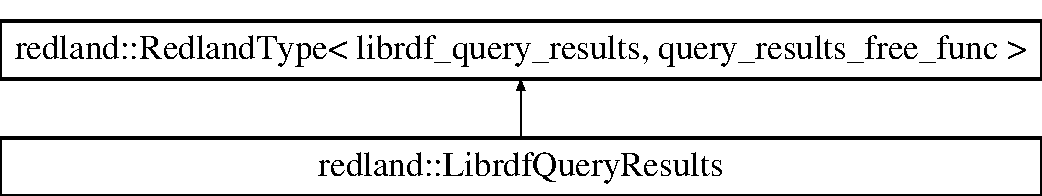
\includegraphics[height=2.000000cm]{classredland_1_1LibrdfQueryResults}
\end{center}
\end{figure}
\doxysubsection*{Public Member Functions}
\begin{DoxyCompactItemize}
\item 
\mbox{\Hypertarget{classredland_1_1LibrdfQueryResults_a8c9e17542c836ff3dd09da68bfc334f1}\label{classredland_1_1LibrdfQueryResults_a8c9e17542c836ff3dd09da68bfc334f1}} 
{\bfseries Librdf\+Query\+Results} (librdf\+\_\+query\+\_\+results $\ast$query\+Results)
\item 
\mbox{\hyperlink{classredland_1_1LibrdfStream}{Librdf\+Stream}} \mbox{\hyperlink{classredland_1_1LibrdfQueryResults_abac7546d8487c786b39046878d27d0b7}{to\+Stream}} ()
\begin{DoxyCompactList}\small\item\em get the query results as a \mbox{\hyperlink{classredland_1_1LibrdfStream}{Librdf\+Stream}} \end{DoxyCompactList}\item 
\mbox{\Hypertarget{classredland_1_1LibrdfQueryResults_a2fc367d8efdeaaa4ebf9e5e710d0440e}\label{classredland_1_1LibrdfQueryResults_a2fc367d8efdeaaa4ebf9e5e710d0440e}} 
int \mbox{\hyperlink{classredland_1_1LibrdfQueryResults_a2fc367d8efdeaaa4ebf9e5e710d0440e}{next}} ()
\begin{DoxyCompactList}\small\item\em Move to the next result. \end{DoxyCompactList}\item 
\mbox{\Hypertarget{classredland_1_1LibrdfQueryResults_ad6ab0b2bd53491ce650f9c740f04c2ec}\label{classredland_1_1LibrdfQueryResults_ad6ab0b2bd53491ce650f9c740f04c2ec}} 
bool \mbox{\hyperlink{classredland_1_1LibrdfQueryResults_ad6ab0b2bd53491ce650f9c740f04c2ec}{is\+Finished}} ()
\begin{DoxyCompactList}\small\item\em true when binding results are exausted \end{DoxyCompactList}\item 
\mbox{\Hypertarget{classredland_1_1LibrdfQueryResults_a1626fe6649dbb8161a05493ac7ec6ee7}\label{classredland_1_1LibrdfQueryResults_a1626fe6649dbb8161a05493ac7ec6ee7}} 
std\+::vector$<$ \mbox{\hyperlink{classredland_1_1LibrdfNode}{Librdf\+Node}} $>$ {\bfseries get\+Bindings} ()
\item 
\mbox{\Hypertarget{classredland_1_1LibrdfQueryResults_a056a92a8cd926072718e4553ed9a39b9}\label{classredland_1_1LibrdfQueryResults_a056a92a8cd926072718e4553ed9a39b9}} 
bool \mbox{\hyperlink{classredland_1_1LibrdfQueryResults_a056a92a8cd926072718e4553ed9a39b9}{is\+Boolean}} ()
\begin{DoxyCompactList}\small\item\em true when this \mbox{\hyperlink{classredland_1_1LibrdfQueryResults}{Librdf\+Query\+Results}} is variable boolean format \end{DoxyCompactList}\item 
\mbox{\Hypertarget{classredland_1_1LibrdfQueryResults_a7a175af6ea28920887c4b2dc4645feb0}\label{classredland_1_1LibrdfQueryResults_a7a175af6ea28920887c4b2dc4645feb0}} 
bool \mbox{\hyperlink{classredland_1_1LibrdfQueryResults_a7a175af6ea28920887c4b2dc4645feb0}{is\+Bindings}} ()
\begin{DoxyCompactList}\small\item\em true when this \mbox{\hyperlink{classredland_1_1LibrdfQueryResults}{Librdf\+Query\+Results}} is variable bindings format \end{DoxyCompactList}\item 
\mbox{\Hypertarget{classredland_1_1LibrdfQueryResults_a52fccc16c398414ddb287fa9bb2a70fd}\label{classredland_1_1LibrdfQueryResults_a52fccc16c398414ddb287fa9bb2a70fd}} 
int {\bfseries get\+Boolean} ()
\item 
\mbox{\Hypertarget{classredland_1_1LibrdfQueryResults_a60e7f4a030655ee3ff0801ce28e3e4e8}\label{classredland_1_1LibrdfQueryResults_a60e7f4a030655ee3ff0801ce28e3e4e8}} 
bool \mbox{\hyperlink{classredland_1_1LibrdfQueryResults_a60e7f4a030655ee3ff0801ce28e3e4e8}{is\+Graph}} ()
\begin{DoxyCompactList}\small\item\em true when this \mbox{\hyperlink{classredland_1_1LibrdfQueryResults}{Librdf\+Query\+Results}} is RDF graph format \end{DoxyCompactList}\item 
\mbox{\Hypertarget{classredland_1_1LibrdfQueryResults_a1a105e783020b8022c5bc8473818be8b}\label{classredland_1_1LibrdfQueryResults_a1a105e783020b8022c5bc8473818be8b}} 
std\+::string {\bfseries get\+Binding\+Value\+By\+Name} (const std\+::string \&name)
\item 
int \mbox{\hyperlink{classredland_1_1LibrdfQueryResults_a1fe7caabdd6e0a2303dd336c9a9b6fb4}{get\+Bindings\+Count}} ()
\begin{DoxyCompactList}\small\item\em returns the number of bindings in the sparql query. \end{DoxyCompactList}\item 
\mbox{\Hypertarget{classredland_1_1LibrdfQueryResults_a6e452fb1c79115834cf97f0898af41f6}\label{classredland_1_1LibrdfQueryResults_a6e452fb1c79115834cf97f0898af41f6}} 
std\+::string {\bfseries to\+String} (const std\+::string \&output\+\_\+format)
\item 
std\+::string \mbox{\hyperlink{classredland_1_1LibrdfQueryResults_ad5f4123f843438e687ef5b8f99816de4}{get\+Bindings\+Name}} (int index)
\begin{DoxyCompactList}\small\item\em get the value of the bindings at \end{DoxyCompactList}\item 
std\+::vector$<$ std\+::string $>$ \mbox{\hyperlink{classredland_1_1LibrdfQueryResults_adf2873cbdc7263b3dd16df61c8ae1c99}{get\+Bindings\+Names}} ()
\begin{DoxyCompactList}\small\item\em get all bindings names as a vector of strings \end{DoxyCompactList}\item 
\mbox{\Hypertarget{classredland_1_1LibrdfQueryResults_a839ea1086c888dbb62c6d5b6d8279add}\label{classredland_1_1LibrdfQueryResults_a839ea1086c888dbb62c6d5b6d8279add}} 
void {\bfseries print\+Query\+Results} ()
\item 
\mbox{\Hypertarget{classredland_1_1LibrdfQueryResults_a856a47ebe225d1d828197f9f2e5c7d9c}\label{classredland_1_1LibrdfQueryResults_a856a47ebe225d1d828197f9f2e5c7d9c}} 
std\+::vector$<$ std\+::string $>$ {\bfseries get\+Valid\+Output\+Formats} () const
\item 
\mbox{\Hypertarget{classredland_1_1LibrdfQueryResults_ac80249e27c57b11309311862c1cee452}\label{classredland_1_1LibrdfQueryResults_ac80249e27c57b11309311862c1cee452}} 
Results\+Map \mbox{\hyperlink{classredland_1_1LibrdfQueryResults_ac80249e27c57b11309311862c1cee452}{map}} ()
\begin{DoxyCompactList}\small\item\em create a map from the query results. \end{DoxyCompactList}\end{DoxyCompactItemize}
\doxysubsection*{Static Public Member Functions}
\begin{DoxyCompactItemize}
\item 
\mbox{\Hypertarget{classredland_1_1LibrdfQueryResults_ad81559675d154f5dd2386ff67d971e46}\label{classredland_1_1LibrdfQueryResults_ad81559675d154f5dd2386ff67d971e46}} 
static std\+::string {\bfseries string\+Replace} (std\+::string str, const std\+::string \&string\+\_\+to\+\_\+replace, const std\+::string \&replacement)
\end{DoxyCompactItemize}
\doxysubsection*{Additional Inherited Members}


\doxysubsection{Member Function Documentation}
\mbox{\Hypertarget{classredland_1_1LibrdfQueryResults_a1fe7caabdd6e0a2303dd336c9a9b6fb4}\label{classredland_1_1LibrdfQueryResults_a1fe7caabdd6e0a2303dd336c9a9b6fb4}} 
\index{redland::LibrdfQueryResults@{redland::LibrdfQueryResults}!getBindingsCount@{getBindingsCount}}
\index{getBindingsCount@{getBindingsCount}!redland::LibrdfQueryResults@{redland::LibrdfQueryResults}}
\doxysubsubsection{\texorpdfstring{getBindingsCount()}{getBindingsCount()}}
{\footnotesize\ttfamily int redland\+::\+Librdf\+Query\+Results\+::get\+Bindings\+Count (\begin{DoxyParamCaption}{ }\end{DoxyParamCaption})}



returns the number of bindings in the sparql query. 

i.\+e. the query SELECT ?x ?y ?z WHERE \{ ?x ?y ?z \} has 3 bindings, x, y and z. \mbox{\Hypertarget{classredland_1_1LibrdfQueryResults_ad5f4123f843438e687ef5b8f99816de4}\label{classredland_1_1LibrdfQueryResults_ad5f4123f843438e687ef5b8f99816de4}} 
\index{redland::LibrdfQueryResults@{redland::LibrdfQueryResults}!getBindingsName@{getBindingsName}}
\index{getBindingsName@{getBindingsName}!redland::LibrdfQueryResults@{redland::LibrdfQueryResults}}
\doxysubsubsection{\texorpdfstring{getBindingsName()}{getBindingsName()}}
{\footnotesize\ttfamily std\+::string redland\+::\+Librdf\+Query\+Results\+::get\+Bindings\+Name (\begin{DoxyParamCaption}\item[{int}]{index }\end{DoxyParamCaption})}



get the value of the bindings at 


\begin{DoxyParams}{Parameters}
{\em index} & as a std\+::string \\
\hline
\end{DoxyParams}
\mbox{\Hypertarget{classredland_1_1LibrdfQueryResults_adf2873cbdc7263b3dd16df61c8ae1c99}\label{classredland_1_1LibrdfQueryResults_adf2873cbdc7263b3dd16df61c8ae1c99}} 
\index{redland::LibrdfQueryResults@{redland::LibrdfQueryResults}!getBindingsNames@{getBindingsNames}}
\index{getBindingsNames@{getBindingsNames}!redland::LibrdfQueryResults@{redland::LibrdfQueryResults}}
\doxysubsubsection{\texorpdfstring{getBindingsNames()}{getBindingsNames()}}
{\footnotesize\ttfamily std\+::vector$<$ std\+::string $>$ redland\+::\+Librdf\+Query\+Results\+::get\+Bindings\+Names (\begin{DoxyParamCaption}{ }\end{DoxyParamCaption})}



get all bindings names as a vector of strings 

the number of bindings is determined by get\+Bindings\+Count \mbox{\Hypertarget{classredland_1_1LibrdfQueryResults_abac7546d8487c786b39046878d27d0b7}\label{classredland_1_1LibrdfQueryResults_abac7546d8487c786b39046878d27d0b7}} 
\index{redland::LibrdfQueryResults@{redland::LibrdfQueryResults}!toStream@{toStream}}
\index{toStream@{toStream}!redland::LibrdfQueryResults@{redland::LibrdfQueryResults}}
\doxysubsubsection{\texorpdfstring{toStream()}{toStream()}}
{\footnotesize\ttfamily \mbox{\hyperlink{classredland_1_1LibrdfStream}{Librdf\+Stream}} redland\+::\+Librdf\+Query\+Results\+::to\+Stream (\begin{DoxyParamCaption}{ }\end{DoxyParamCaption})}



get the query results as a \mbox{\hyperlink{classredland_1_1LibrdfStream}{Librdf\+Stream}} 

only meaningful if this is an RDF graph query result 
\begin{DoxyExceptions}{Exceptions}
{\em invalid\+\_\+argument} & when to\+Stream is called and Librdf\+Query\+Result\+::is\+Graph() evaluates to false. \\
\hline
\end{DoxyExceptions}


The documentation for this class was generated from the following files\+:\begin{DoxyCompactItemize}
\item 
src/redland/\+Redland\+Wrapper/src/include/redland/Librdf\+Query\+Results.\+h\item 
src/redland/\+Redland\+Wrapper/src/Librdf\+Query\+Results.\+cpp\end{DoxyCompactItemize}

\hypertarget{classredland_1_1LibrdfSerializer}{}\doxysection{redland\+::Librdf\+Serializer Class Reference}
\label{classredland_1_1LibrdfSerializer}\index{redland::LibrdfSerializer@{redland::LibrdfSerializer}}
\doxysubsection*{Public Member Functions}
\begin{DoxyCompactItemize}
\item 
\mbox{\Hypertarget{classredland_1_1LibrdfSerializer_a084920f2dadf9aff9abff2fbe4e302e9}\label{classredland_1_1LibrdfSerializer_a084920f2dadf9aff9abff2fbe4e302e9}} 
{\bfseries Librdf\+Serializer} (const \mbox{\hyperlink{classredland_1_1LibrdfSerializer}{Librdf\+Serializer}} \&serializer)=delete
\item 
\mbox{\Hypertarget{classredland_1_1LibrdfSerializer_ac0df7aa8f6a63de75d63f33d9eb3b201}\label{classredland_1_1LibrdfSerializer_ac0df7aa8f6a63de75d63f33d9eb3b201}} 
{\bfseries Librdf\+Serializer} (\mbox{\hyperlink{classredland_1_1LibrdfSerializer}{Librdf\+Serializer}} \&\&serializer) noexcept
\item 
\mbox{\Hypertarget{classredland_1_1LibrdfSerializer_a07c9ec356305e42c4990357dffb6bfd1}\label{classredland_1_1LibrdfSerializer_a07c9ec356305e42c4990357dffb6bfd1}} 
\mbox{\hyperlink{classredland_1_1LibrdfSerializer}{Librdf\+Serializer}} \& {\bfseries operator=} (const \mbox{\hyperlink{classredland_1_1LibrdfSerializer}{Librdf\+Serializer}} \&serializer)=delete
\item 
\mbox{\Hypertarget{classredland_1_1LibrdfSerializer_a3f1049838f6c9b3baee42fd1ab99d9e3}\label{classredland_1_1LibrdfSerializer_a3f1049838f6c9b3baee42fd1ab99d9e3}} 
\mbox{\hyperlink{classredland_1_1LibrdfSerializer}{Librdf\+Serializer}} \& {\bfseries operator=} (\mbox{\hyperlink{classredland_1_1LibrdfSerializer}{Librdf\+Serializer}} \&\&serializer) noexcept
\item 
\mbox{\Hypertarget{classredland_1_1LibrdfSerializer_aadcc241a243f87fce5152dc6420d1625}\label{classredland_1_1LibrdfSerializer_aadcc241a243f87fce5152dc6420d1625}} 
{\bfseries Librdf\+Serializer} (const char $\ast$format, const char $\ast$mime\+\_\+type=nullptr, const char $\ast$type\+\_\+uri=nullptr)
\item 
\mbox{\Hypertarget{classredland_1_1LibrdfSerializer_ab5ef7eaa294357a931b826acc1ab932f}\label{classredland_1_1LibrdfSerializer_ab5ef7eaa294357a931b826acc1ab932f}} 
librdf\+\_\+serializer $\ast$ {\bfseries get} () const
\item 
\mbox{\Hypertarget{classredland_1_1LibrdfSerializer_ab621a575b7244c9d39e756b5e133766b}\label{classredland_1_1LibrdfSerializer_ab621a575b7244c9d39e756b5e133766b}} 
void {\bfseries set\+Namespace} (const std\+::string \&ns, const std\+::string \&prefix) const
\item 
\mbox{\Hypertarget{classredland_1_1LibrdfSerializer_abe500f5c5a1de1bdac86ab196a002b46}\label{classredland_1_1LibrdfSerializer_abe500f5c5a1de1bdac86ab196a002b46}} 
void {\bfseries set\+Feature} (const std\+::string \&ns, const std\+::string \&prefix) const
\item 
\mbox{\Hypertarget{classredland_1_1LibrdfSerializer_ac205990ca1dbf0ff1e56ea45e82ec8d2}\label{classredland_1_1LibrdfSerializer_ac205990ca1dbf0ff1e56ea45e82ec8d2}} 
std\+::string {\bfseries to\+String} (const std\+::string \&uri, const \mbox{\hyperlink{classredland_1_1LibrdfModel}{Librdf\+Model}} \&model)
\item 
\mbox{\Hypertarget{classredland_1_1LibrdfSerializer_aa185a5c5708bf4b08dfa5eb6a8b897b1}\label{classredland_1_1LibrdfSerializer_aa185a5c5708bf4b08dfa5eb6a8b897b1}} 
void {\bfseries free\+Serializer} ()
\item 
\mbox{\Hypertarget{classredland_1_1LibrdfSerializer_a4ea50f1f63c3cb7bb63da3fc55994fee}\label{classredland_1_1LibrdfSerializer_a4ea50f1f63c3cb7bb63da3fc55994fee}} 
void {\bfseries validate\+Serializer\+Name} (std\+::string name)
\item 
\mbox{\Hypertarget{classredland_1_1LibrdfSerializer_a970fa3d23ba08a63533c758417de1808}\label{classredland_1_1LibrdfSerializer_a970fa3d23ba08a63533c758417de1808}} 
void {\bfseries set\+Option} (const std\+::string \&option, const std\+::string \&value) const
\item 
\mbox{\Hypertarget{classredland_1_1LibrdfSerializer_ad2cb2ddcd225119a2a9a33001da22478}\label{classredland_1_1LibrdfSerializer_ad2cb2ddcd225119a2a9a33001da22478}} 
void {\bfseries set\+Options} () const
\end{DoxyCompactItemize}
\doxysubsection*{Static Public Member Functions}
\begin{DoxyCompactItemize}
\item 
\mbox{\Hypertarget{classredland_1_1LibrdfSerializer_a58915bb2aa6b7c0eb438b5cc0148ef45}\label{classredland_1_1LibrdfSerializer_a58915bb2aa6b7c0eb438b5cc0148ef45}} 
static \mbox{\hyperlink{classredland_1_1LibrdfSerializer}{Librdf\+Serializer}} {\bfseries from\+Raw\+Ptr} (librdf\+\_\+serializer $\ast$serializer)
\end{DoxyCompactItemize}


The documentation for this class was generated from the following files\+:\begin{DoxyCompactItemize}
\item 
src/redland/\+Redland\+Wrapper/src/Librdf\+Serializer.\+h\item 
src/redland/\+Redland\+Wrapper/src/Librdf\+Serializer.\+cpp\end{DoxyCompactItemize}

\hypertarget{classredland_1_1LibrdfStatement}{}\doxysection{redland\+::Librdf\+Statement Class Reference}
\label{classredland_1_1LibrdfStatement}\index{redland::LibrdfStatement@{redland::LibrdfStatement}}


C++ wrapper around librdf\+\_\+statement using RAII for memory management.  




{\ttfamily \#include $<$Librdf\+Statement.\+h$>$}

Inheritance diagram for redland\+::Librdf\+Statement\+:\begin{figure}[H]
\begin{center}
\leavevmode
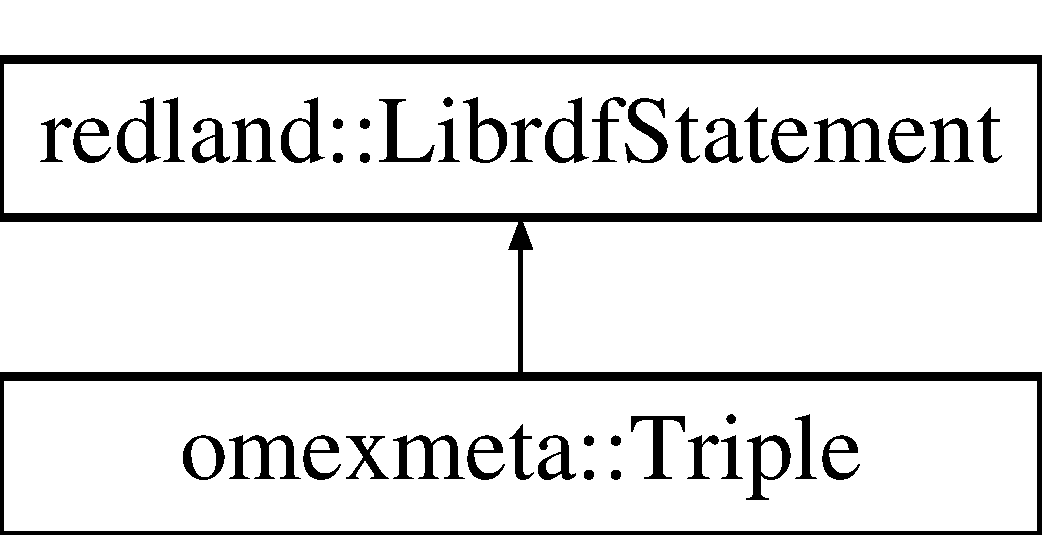
\includegraphics[height=4.000000cm]{classredland_1_1LibrdfStatement}
\end{center}
\end{figure}
\doxysubsection*{Public Member Functions}
\begin{DoxyCompactItemize}
\item 
\mbox{\hyperlink{classredland_1_1LibrdfStatement_a4cbbbf99d094cea4569324a8c67789fb}{Librdf\+Statement}} (\mbox{\hyperlink{structraptor__statement}{librdf\+\_\+statement}} $\ast$statement)
\begin{DoxyCompactList}\small\item\em construct a \mbox{\hyperlink{classredland_1_1LibrdfStatement}{Librdf\+Statement}} from an existing librdf\+\_\+statement$\ast$ pointer. \end{DoxyCompactList}\item 
\mbox{\hyperlink{classredland_1_1LibrdfStatement_a65d896e0bf026ff027ad8488bddf6384}{Librdf\+Statement}} ()
\begin{DoxyCompactList}\small\item\em default construct an instance of librdf\+\_\+statement$\ast$. \end{DoxyCompactList}\item 
\mbox{\Hypertarget{classredland_1_1LibrdfStatement_ada81e9bfb312e25daf20d6dda10eeb2e}\label{classredland_1_1LibrdfStatement_ada81e9bfb312e25daf20d6dda10eeb2e}} 
bool \mbox{\hyperlink{classredland_1_1LibrdfStatement_ada81e9bfb312e25daf20d6dda10eeb2e}{operator==}} (const \mbox{\hyperlink{classredland_1_1LibrdfStatement}{Librdf\+Statement}} \&rhs) const
\begin{DoxyCompactList}\small\item\em equality operator. @detials equal if the three nodes contained by this statement are equal \end{DoxyCompactList}\item 
\mbox{\Hypertarget{classredland_1_1LibrdfStatement_ad3d6c126b90c0d93413a08353c496f8f}\label{classredland_1_1LibrdfStatement_ad3d6c126b90c0d93413a08353c496f8f}} 
bool \mbox{\hyperlink{classredland_1_1LibrdfStatement_ad3d6c126b90c0d93413a08353c496f8f}{operator!=}} (const \mbox{\hyperlink{classredland_1_1LibrdfStatement}{Librdf\+Statement}} \&rhs) const
\begin{DoxyCompactList}\small\item\em inequality operator. Inverse of equality operator \end{DoxyCompactList}\item 
\mbox{\hyperlink{classredland_1_1LibrdfStatement_ae7f7e27b7a502070195103268407243a}{Librdf\+Statement}} (const \mbox{\hyperlink{classredland_1_1LibrdfNode}{Librdf\+Node}} \&subject, const \mbox{\hyperlink{classredland_1_1LibrdfNode}{Librdf\+Node}} \&predicate, const \mbox{\hyperlink{classredland_1_1LibrdfNode}{Librdf\+Node}} \&resource)
\begin{DoxyCompactList}\small\item\em construct a \mbox{\hyperlink{classredland_1_1LibrdfStatement}{Librdf\+Statement}} from \mbox{\hyperlink{classredland_1_1LibrdfNode}{Librdf\+Node}} objects. \end{DoxyCompactList}\item 
\mbox{\hyperlink{classredland_1_1LibrdfNode}{Librdf\+Node}} \mbox{\hyperlink{classredland_1_1LibrdfStatement_a2d7cc313572ac34e9822e97d6b23dd36}{get\+Subject\+Node}} () const
\begin{DoxyCompactList}\small\item\em get the subject of this statement as a \mbox{\hyperlink{classredland_1_1LibrdfNode}{Librdf\+Node}}. \end{DoxyCompactList}\item 
\mbox{\hyperlink{classredland_1_1LibrdfNode}{Librdf\+Node}} \mbox{\hyperlink{classredland_1_1LibrdfStatement_ade668892ca9383eacbf5517df4e8f8d8}{get\+Predicate\+Node}} () const
\begin{DoxyCompactList}\small\item\em get the predicate of this statement as a \mbox{\hyperlink{classredland_1_1LibrdfNode}{Librdf\+Node}}. \end{DoxyCompactList}\item 
\mbox{\hyperlink{classredland_1_1LibrdfNode}{Librdf\+Node}} \mbox{\hyperlink{classredland_1_1LibrdfStatement_a9d4376221d84e22d15eeb6393ea4afe3}{get\+Resource\+Node}} () const
\begin{DoxyCompactList}\small\item\em get the resource of this statement as a \mbox{\hyperlink{classredland_1_1LibrdfNode}{Librdf\+Node}}. \end{DoxyCompactList}\item 
\mbox{\Hypertarget{classredland_1_1LibrdfStatement_a4935cf54fa2f367678319f1f2d837005}\label{classredland_1_1LibrdfStatement_a4935cf54fa2f367678319f1f2d837005}} 
void \mbox{\hyperlink{classredland_1_1LibrdfStatement_a4935cf54fa2f367678319f1f2d837005}{check\+For\+Null}} () override
\begin{DoxyCompactList}\small\item\em throws an error if any of the subject, predicate, resource or librdf\+\_\+statement are nullptr. \end{DoxyCompactList}\item 
void \mbox{\hyperlink{classredland_1_1LibrdfStatement_a9133d53a9b24ac0f0499f23cb6e53d40}{set\+Subject}} (const \mbox{\hyperlink{classredland_1_1LibrdfNode}{Librdf\+Node}} \&node)
\begin{DoxyCompactList}\small\item\em set the subject of this \mbox{\hyperlink{classredland_1_1LibrdfStatement}{Librdf\+Statement}} to node. \end{DoxyCompactList}\item 
void \mbox{\hyperlink{classredland_1_1LibrdfStatement_a74151d5fae756918cfd9b22d51fb8d71}{set\+Resource}} (const \mbox{\hyperlink{classredland_1_1LibrdfNode}{Librdf\+Node}} \&node)
\begin{DoxyCompactList}\small\item\em set the resource of this \mbox{\hyperlink{classredland_1_1LibrdfStatement}{Librdf\+Statement}} to node. \end{DoxyCompactList}\item 
void \mbox{\hyperlink{classredland_1_1LibrdfStatement_a155e25bff7660b03c4253715fe5e8194}{set\+Predicate}} (const \mbox{\hyperlink{classredland_1_1LibrdfNode}{Librdf\+Node}} \&node)
\begin{DoxyCompactList}\small\item\em set the predicate of this \mbox{\hyperlink{classredland_1_1LibrdfStatement}{Librdf\+Statement}} to node. \end{DoxyCompactList}\item 
\mbox{\Hypertarget{classredland_1_1LibrdfStatement_a84a6fae7f1879c2f033001a9927627b0}\label{classredland_1_1LibrdfStatement_a84a6fae7f1879c2f033001a9927627b0}} 
bool \mbox{\hyperlink{classredland_1_1LibrdfStatement_a84a6fae7f1879c2f033001a9927627b0}{is\+Complete}} ()
\begin{DoxyCompactList}\small\item\em returns true when all of subject, predicate and resource nodes are not empty. \end{DoxyCompactList}\end{DoxyCompactItemize}
\doxysubsection*{Static Public Member Functions}
\begin{DoxyCompactItemize}
\item 
static bool \mbox{\hyperlink{classredland_1_1LibrdfStatement_ac5acd1a9c67a8bd6f7b99098a7353424}{equals}} (const \mbox{\hyperlink{classredland_1_1LibrdfStatement}{Librdf\+Statement}} \&first, const \mbox{\hyperlink{classredland_1_1LibrdfStatement}{Librdf\+Statement}} \&second)
\begin{DoxyCompactList}\small\item\em returns true if first equals second. \end{DoxyCompactList}\end{DoxyCompactItemize}
\doxysubsection*{Additional Inherited Members}


\doxysubsection{Detailed Description}
C++ wrapper around librdf\+\_\+statement using RAII for memory management. 

\doxysubsection{Constructor \& Destructor Documentation}
\mbox{\Hypertarget{classredland_1_1LibrdfStatement_a4cbbbf99d094cea4569324a8c67789fb}\label{classredland_1_1LibrdfStatement_a4cbbbf99d094cea4569324a8c67789fb}} 
\index{redland::LibrdfStatement@{redland::LibrdfStatement}!LibrdfStatement@{LibrdfStatement}}
\index{LibrdfStatement@{LibrdfStatement}!redland::LibrdfStatement@{redland::LibrdfStatement}}
\doxysubsubsection{\texorpdfstring{LibrdfStatement()}{LibrdfStatement()}\hspace{0.1cm}{\footnotesize\ttfamily [1/3]}}
{\footnotesize\ttfamily redland\+::\+Librdf\+Statement\+::\+Librdf\+Statement (\begin{DoxyParamCaption}\item[{\mbox{\hyperlink{structraptor__statement}{librdf\+\_\+statement}} $\ast$}]{statement }\end{DoxyParamCaption})\hspace{0.3cm}{\ttfamily [explicit]}}



construct a \mbox{\hyperlink{classredland_1_1LibrdfStatement}{Librdf\+Statement}} from an existing librdf\+\_\+statement$\ast$ pointer. 

The reference is stolen, and subsequently managed by \mbox{\hyperlink{classredland_1_1LibrdfStatement}{Librdf\+Statement}} \mbox{\Hypertarget{classredland_1_1LibrdfStatement_a65d896e0bf026ff027ad8488bddf6384}\label{classredland_1_1LibrdfStatement_a65d896e0bf026ff027ad8488bddf6384}} 
\index{redland::LibrdfStatement@{redland::LibrdfStatement}!LibrdfStatement@{LibrdfStatement}}
\index{LibrdfStatement@{LibrdfStatement}!redland::LibrdfStatement@{redland::LibrdfStatement}}
\doxysubsubsection{\texorpdfstring{LibrdfStatement()}{LibrdfStatement()}\hspace{0.1cm}{\footnotesize\ttfamily [2/3]}}
{\footnotesize\ttfamily redland\+::\+Librdf\+Statement\+::\+Librdf\+Statement (\begin{DoxyParamCaption}{ }\end{DoxyParamCaption})}



default construct an instance of librdf\+\_\+statement$\ast$. 

Memory is owned by \mbox{\hyperlink{classredland_1_1LibrdfStatement}{Librdf\+Statement}} and automatically destructed via RAII. \mbox{\Hypertarget{classredland_1_1LibrdfStatement_ae7f7e27b7a502070195103268407243a}\label{classredland_1_1LibrdfStatement_ae7f7e27b7a502070195103268407243a}} 
\index{redland::LibrdfStatement@{redland::LibrdfStatement}!LibrdfStatement@{LibrdfStatement}}
\index{LibrdfStatement@{LibrdfStatement}!redland::LibrdfStatement@{redland::LibrdfStatement}}
\doxysubsubsection{\texorpdfstring{LibrdfStatement()}{LibrdfStatement()}\hspace{0.1cm}{\footnotesize\ttfamily [3/3]}}
{\footnotesize\ttfamily redland\+::\+Librdf\+Statement\+::\+Librdf\+Statement (\begin{DoxyParamCaption}\item[{const \mbox{\hyperlink{classredland_1_1LibrdfNode}{Librdf\+Node}} \&}]{subject,  }\item[{const \mbox{\hyperlink{classredland_1_1LibrdfNode}{Librdf\+Node}} \&}]{predicate,  }\item[{const \mbox{\hyperlink{classredland_1_1LibrdfNode}{Librdf\+Node}} \&}]{resource }\end{DoxyParamCaption})}



construct a \mbox{\hyperlink{classredland_1_1LibrdfStatement}{Librdf\+Statement}} from \mbox{\hyperlink{classredland_1_1LibrdfNode}{Librdf\+Node}} objects. 

The memory associated with the constructed librdf\+\_\+statement$\ast$ is managed by RAII while the \mbox{\hyperlink{classredland_1_1LibrdfNode}{Librdf\+Node}} types handled themselves, also by RAII. The reference count of the \mbox{\hyperlink{classredland_1_1LibrdfNode}{Librdf\+Node}} types is incremented by 1 on instantiation 

\doxysubsection{Member Function Documentation}
\mbox{\Hypertarget{classredland_1_1LibrdfStatement_ac5acd1a9c67a8bd6f7b99098a7353424}\label{classredland_1_1LibrdfStatement_ac5acd1a9c67a8bd6f7b99098a7353424}} 
\index{redland::LibrdfStatement@{redland::LibrdfStatement}!equals@{equals}}
\index{equals@{equals}!redland::LibrdfStatement@{redland::LibrdfStatement}}
\doxysubsubsection{\texorpdfstring{equals()}{equals()}}
{\footnotesize\ttfamily bool redland\+::\+Librdf\+Statement\+::equals (\begin{DoxyParamCaption}\item[{const \mbox{\hyperlink{classredland_1_1LibrdfStatement}{Librdf\+Statement}} \&}]{first,  }\item[{const \mbox{\hyperlink{classredland_1_1LibrdfStatement}{Librdf\+Statement}} \&}]{second }\end{DoxyParamCaption})\hspace{0.3cm}{\ttfamily [static]}}



returns true if first equals second. 

All three of subject, predicate and resource nodes need to be equal before \mbox{\hyperlink{classredland_1_1LibrdfStatement_ac5acd1a9c67a8bd6f7b99098a7353424}{Librdf\+Statement\+::equals}} returns true. \mbox{\Hypertarget{classredland_1_1LibrdfStatement_ade668892ca9383eacbf5517df4e8f8d8}\label{classredland_1_1LibrdfStatement_ade668892ca9383eacbf5517df4e8f8d8}} 
\index{redland::LibrdfStatement@{redland::LibrdfStatement}!getPredicateNode@{getPredicateNode}}
\index{getPredicateNode@{getPredicateNode}!redland::LibrdfStatement@{redland::LibrdfStatement}}
\doxysubsubsection{\texorpdfstring{getPredicateNode()}{getPredicateNode()}}
{\footnotesize\ttfamily \mbox{\hyperlink{classredland_1_1LibrdfNode}{Librdf\+Node}} redland\+::\+Librdf\+Statement\+::get\+Predicate\+Node (\begin{DoxyParamCaption}{ }\end{DoxyParamCaption}) const}



get the predicate of this statement as a \mbox{\hyperlink{classredland_1_1LibrdfNode}{Librdf\+Node}}. 

Ref count is incremented by 1 \mbox{\Hypertarget{classredland_1_1LibrdfStatement_a9d4376221d84e22d15eeb6393ea4afe3}\label{classredland_1_1LibrdfStatement_a9d4376221d84e22d15eeb6393ea4afe3}} 
\index{redland::LibrdfStatement@{redland::LibrdfStatement}!getResourceNode@{getResourceNode}}
\index{getResourceNode@{getResourceNode}!redland::LibrdfStatement@{redland::LibrdfStatement}}
\doxysubsubsection{\texorpdfstring{getResourceNode()}{getResourceNode()}}
{\footnotesize\ttfamily \mbox{\hyperlink{classredland_1_1LibrdfNode}{Librdf\+Node}} redland\+::\+Librdf\+Statement\+::get\+Resource\+Node (\begin{DoxyParamCaption}{ }\end{DoxyParamCaption}) const}



get the resource of this statement as a \mbox{\hyperlink{classredland_1_1LibrdfNode}{Librdf\+Node}}. 

Ref count is incremented by 1 \mbox{\Hypertarget{classredland_1_1LibrdfStatement_a2d7cc313572ac34e9822e97d6b23dd36}\label{classredland_1_1LibrdfStatement_a2d7cc313572ac34e9822e97d6b23dd36}} 
\index{redland::LibrdfStatement@{redland::LibrdfStatement}!getSubjectNode@{getSubjectNode}}
\index{getSubjectNode@{getSubjectNode}!redland::LibrdfStatement@{redland::LibrdfStatement}}
\doxysubsubsection{\texorpdfstring{getSubjectNode()}{getSubjectNode()}}
{\footnotesize\ttfamily \mbox{\hyperlink{classredland_1_1LibrdfNode}{Librdf\+Node}} redland\+::\+Librdf\+Statement\+::get\+Subject\+Node (\begin{DoxyParamCaption}{ }\end{DoxyParamCaption}) const}



get the subject of this statement as a \mbox{\hyperlink{classredland_1_1LibrdfNode}{Librdf\+Node}}. 

Ref count is incremented by 1 \mbox{\Hypertarget{classredland_1_1LibrdfStatement_a155e25bff7660b03c4253715fe5e8194}\label{classredland_1_1LibrdfStatement_a155e25bff7660b03c4253715fe5e8194}} 
\index{redland::LibrdfStatement@{redland::LibrdfStatement}!setPredicate@{setPredicate}}
\index{setPredicate@{setPredicate}!redland::LibrdfStatement@{redland::LibrdfStatement}}
\doxysubsubsection{\texorpdfstring{setPredicate()}{setPredicate()}}
{\footnotesize\ttfamily void redland\+::\+Librdf\+Statement\+::set\+Predicate (\begin{DoxyParamCaption}\item[{const \mbox{\hyperlink{classredland_1_1LibrdfNode}{Librdf\+Node}} \&}]{node }\end{DoxyParamCaption})}



set the predicate of this \mbox{\hyperlink{classredland_1_1LibrdfStatement}{Librdf\+Statement}} to node. 

reference count of node is incremented \mbox{\Hypertarget{classredland_1_1LibrdfStatement_a74151d5fae756918cfd9b22d51fb8d71}\label{classredland_1_1LibrdfStatement_a74151d5fae756918cfd9b22d51fb8d71}} 
\index{redland::LibrdfStatement@{redland::LibrdfStatement}!setResource@{setResource}}
\index{setResource@{setResource}!redland::LibrdfStatement@{redland::LibrdfStatement}}
\doxysubsubsection{\texorpdfstring{setResource()}{setResource()}}
{\footnotesize\ttfamily void redland\+::\+Librdf\+Statement\+::set\+Resource (\begin{DoxyParamCaption}\item[{const \mbox{\hyperlink{classredland_1_1LibrdfNode}{Librdf\+Node}} \&}]{node }\end{DoxyParamCaption})}



set the resource of this \mbox{\hyperlink{classredland_1_1LibrdfStatement}{Librdf\+Statement}} to node. 

reference count of node is incremented \mbox{\Hypertarget{classredland_1_1LibrdfStatement_a9133d53a9b24ac0f0499f23cb6e53d40}\label{classredland_1_1LibrdfStatement_a9133d53a9b24ac0f0499f23cb6e53d40}} 
\index{redland::LibrdfStatement@{redland::LibrdfStatement}!setSubject@{setSubject}}
\index{setSubject@{setSubject}!redland::LibrdfStatement@{redland::LibrdfStatement}}
\doxysubsubsection{\texorpdfstring{setSubject()}{setSubject()}}
{\footnotesize\ttfamily void redland\+::\+Librdf\+Statement\+::set\+Subject (\begin{DoxyParamCaption}\item[{const \mbox{\hyperlink{classredland_1_1LibrdfNode}{Librdf\+Node}} \&}]{node }\end{DoxyParamCaption})}



set the subject of this \mbox{\hyperlink{classredland_1_1LibrdfStatement}{Librdf\+Statement}} to node. 

reference count of node is incremented 

The documentation for this class was generated from the following files\+:\begin{DoxyCompactItemize}
\item 
src/redland/\+Redland\+Wrapper/src/include/redland/Librdf\+Statement.\+h\item 
src/redland/\+Redland\+Wrapper/src/Librdf\+Statement.\+cpp\end{DoxyCompactItemize}

\hypertarget{classredland_1_1LibrdfStorage}{}\section{redland\+:\+:Librdf\+Storage Class Reference}
\label{classredland_1_1LibrdfStorage}\index{redland\+::\+Librdf\+Storage@{redland\+::\+Librdf\+Storage}}
\subsection*{Public Member Functions}
\begin{DoxyCompactItemize}
\item 
\mbox{\Hypertarget{classredland_1_1LibrdfStorage_a8e3250af4dea528dcf94865835cfb8ff}\label{classredland_1_1LibrdfStorage_a8e3250af4dea528dcf94865835cfb8ff}} 
{\bfseries Librdf\+Storage} (librdf\+\_\+storage $\ast$storage)
\item 
\mbox{\Hypertarget{classredland_1_1LibrdfStorage_a08c025b165113efe1163c7294b989755}\label{classredland_1_1LibrdfStorage_a08c025b165113efe1163c7294b989755}} 
{\bfseries Librdf\+Storage} (const std\+::string \&storage\+\_\+name=\char`\"{}memory\char`\"{}, const std\+::string \&name=\char`\"{}Semsim\+Store\char`\"{}, const char $\ast$options=nullptr)
\item 
\mbox{\Hypertarget{classredland_1_1LibrdfStorage_a182d617ba7ab1b5359ef2693a56b272e}\label{classredland_1_1LibrdfStorage_a182d617ba7ab1b5359ef2693a56b272e}} 
librdf\+\_\+storage $\ast$ {\bfseries get} () const
\item 
\mbox{\Hypertarget{classredland_1_1LibrdfStorage_a7b08e7afd5ac5f38a0ed4cfeb77a3b99}\label{classredland_1_1LibrdfStorage_a7b08e7afd5ac5f38a0ed4cfeb77a3b99}} 
void {\bfseries free\+Storage} ()
\item 
\mbox{\Hypertarget{classredland_1_1LibrdfStorage_a7cef1518384fd6592ee8521cb95eb25d}\label{classredland_1_1LibrdfStorage_a7cef1518384fd6592ee8521cb95eb25d}} 
{\bfseries Librdf\+Storage} (const \hyperlink{classredland_1_1LibrdfStorage}{Librdf\+Storage} \&storage)=delete
\item 
\mbox{\Hypertarget{classredland_1_1LibrdfStorage_a59184a87b901f1d3709d045d57311606}\label{classredland_1_1LibrdfStorage_a59184a87b901f1d3709d045d57311606}} 
{\bfseries Librdf\+Storage} (\hyperlink{classredland_1_1LibrdfStorage}{Librdf\+Storage} \&\&storage) noexcept
\item 
\mbox{\Hypertarget{classredland_1_1LibrdfStorage_a1366716bbd3a0e41979d632c532c71ec}\label{classredland_1_1LibrdfStorage_a1366716bbd3a0e41979d632c532c71ec}} 
\hyperlink{classredland_1_1LibrdfStorage}{Librdf\+Storage} \& {\bfseries operator=} (\hyperlink{classredland_1_1LibrdfStorage}{Librdf\+Storage} \&\&storage) noexcept
\item 
\mbox{\Hypertarget{classredland_1_1LibrdfStorage_a3782ab4a08a32bd23a38eaad9c980fe9}\label{classredland_1_1LibrdfStorage_a3782ab4a08a32bd23a38eaad9c980fe9}} 
int {\bfseries add\+Statement} (librdf\+\_\+statement $\ast$statement)
\item 
\mbox{\Hypertarget{classredland_1_1LibrdfStorage_ae5e7a3708936893c9e553cbdc23d643a}\label{classredland_1_1LibrdfStorage_ae5e7a3708936893c9e553cbdc23d643a}} 
int {\bfseries add\+Statement} (const \hyperlink{classredland_1_1LibrdfStatement}{Librdf\+Statement} \&statement)
\item 
\mbox{\Hypertarget{classredland_1_1LibrdfStorage_a31ecaace536dface7d4a667ccf8db06c}\label{classredland_1_1LibrdfStorage_a31ecaace536dface7d4a667ccf8db06c}} 
int {\bfseries size} ()
\item 
\mbox{\Hypertarget{classredland_1_1LibrdfStorage_afb361eb4addaf74b725d63fed2cb38e6}\label{classredland_1_1LibrdfStorage_afb361eb4addaf74b725d63fed2cb38e6}} 
int {\bfseries commit} ()
\item 
\mbox{\Hypertarget{classredland_1_1LibrdfStorage_a93cc1f3c7e7ff2a250c9b14f66f60e39}\label{classredland_1_1LibrdfStorage_a93cc1f3c7e7ff2a250c9b14f66f60e39}} 
void {\bfseries print\+Available\+Storages} ()
\end{DoxyCompactItemize}


The documentation for this class was generated from the following files\+:\begin{DoxyCompactItemize}
\item 
src/redland/\+Redland\+Wrapper/src/Librdf\+Storage.\+h\item 
src/redland/\+Redland\+Wrapper/src/Librdf\+Storage.\+cpp\end{DoxyCompactItemize}

\hypertarget{classredland_1_1LibrdfStream}{}\section{redland\+:\+:Librdf\+Stream Class Reference}
\label{classredland_1_1LibrdfStream}\index{redland\+::\+Librdf\+Stream@{redland\+::\+Librdf\+Stream}}
\subsection*{Public Member Functions}
\begin{DoxyCompactItemize}
\item 
\mbox{\Hypertarget{classredland_1_1LibrdfStream_aaa64a7ef8a26be8cf35f3b31d6e34a1b}\label{classredland_1_1LibrdfStream_aaa64a7ef8a26be8cf35f3b31d6e34a1b}} 
{\bfseries Librdf\+Stream} (librdf\+\_\+stream $\ast$stream)
\item 
\mbox{\Hypertarget{classredland_1_1LibrdfStream_a5b52659abdfc01e583e1b9941eec2c4b}\label{classredland_1_1LibrdfStream_a5b52659abdfc01e583e1b9941eec2c4b}} 
librdf\+\_\+stream $\ast$ {\bfseries get} () const
\end{DoxyCompactItemize}


The documentation for this class was generated from the following files\+:\begin{DoxyCompactItemize}
\item 
src/redland/\+Redland\+A\+P\+I\+Wrapper/src/Librdf\+Stream.\+h\item 
src/redland/\+Redland\+A\+P\+I\+Wrapper/src/Librdf\+Stream.\+cpp\end{DoxyCompactItemize}

\hypertarget{classredland_1_1LibrdfUri}{}\doxysection{redland\+::Librdf\+Uri Class Reference}
\label{classredland_1_1LibrdfUri}\index{redland::LibrdfUri@{redland::LibrdfUri}}
\doxysubsection*{Public Member Functions}
\begin{DoxyCompactItemize}
\item 
\mbox{\Hypertarget{classredland_1_1LibrdfUri_a3630cf904c9e4546fb6d6c175ed6c66e}\label{classredland_1_1LibrdfUri_a3630cf904c9e4546fb6d6c175ed6c66e}} 
\mbox{\hyperlink{classredland_1_1LibrdfUri}{Librdf\+Uri}} {\bfseries concatonate} (const std\+::string \&local\+\_\+name) const
\item 
\mbox{\Hypertarget{classredland_1_1LibrdfUri_acaeb8a0d4b6f493805ecc1b198807e1c}\label{classredland_1_1LibrdfUri_acaeb8a0d4b6f493805ecc1b198807e1c}} 
std\+::string {\bfseries str} () const
\item 
\mbox{\Hypertarget{classredland_1_1LibrdfUri_a36c5c589ae207ad6294e10be2bb8df17}\label{classredland_1_1LibrdfUri_a36c5c589ae207ad6294e10be2bb8df17}} 
{\bfseries Librdf\+Uri} (const std\+::string \&uri)
\item 
\mbox{\Hypertarget{classredland_1_1LibrdfUri_a1858bf7c3afae7d6d8ed2dca47e9cf55}\label{classredland_1_1LibrdfUri_a1858bf7c3afae7d6d8ed2dca47e9cf55}} 
librdf\+\_\+uri $\ast$ {\bfseries get} () const
\item 
\mbox{\Hypertarget{classredland_1_1LibrdfUri_ae9a8237bcb9cba0f2d87f2d980f579f3}\label{classredland_1_1LibrdfUri_ae9a8237bcb9cba0f2d87f2d980f579f3}} 
bool {\bfseries is\+Null} () const
\item 
\mbox{\Hypertarget{classredland_1_1LibrdfUri_a13f1a7bc775cd79b6bb4dc6cd31b5d53}\label{classredland_1_1LibrdfUri_a13f1a7bc775cd79b6bb4dc6cd31b5d53}} 
bool {\bfseries is\+Empty} () const
\item 
\mbox{\Hypertarget{classredland_1_1LibrdfUri_aa07e6315dc3428b6d864deb00cda48e1}\label{classredland_1_1LibrdfUri_aa07e6315dc3428b6d864deb00cda48e1}} 
void {\bfseries free\+Uri} ()
\item 
\mbox{\Hypertarget{classredland_1_1LibrdfUri_a770d47b63c041e39761f8dd46b0bf8b5}\label{classredland_1_1LibrdfUri_a770d47b63c041e39761f8dd46b0bf8b5}} 
bool {\bfseries is\+File\+Uri} () const
\item 
\mbox{\Hypertarget{classredland_1_1LibrdfUri_a02d802c21de7c9dba4133779701e3a45}\label{classredland_1_1LibrdfUri_a02d802c21de7c9dba4133779701e3a45}} 
bool {\bfseries operator==} (const \mbox{\hyperlink{classredland_1_1LibrdfUri}{Librdf\+Uri}} \&rhs) const
\item 
\mbox{\Hypertarget{classredland_1_1LibrdfUri_a8ded118526be9cfdbe6dbc87d075fb06}\label{classredland_1_1LibrdfUri_a8ded118526be9cfdbe6dbc87d075fb06}} 
bool {\bfseries operator!=} (const \mbox{\hyperlink{classredland_1_1LibrdfUri}{Librdf\+Uri}} \&rhs) const
\item 
\mbox{\Hypertarget{classredland_1_1LibrdfUri_ad24448f9b22adce080a35decc4694479}\label{classredland_1_1LibrdfUri_ad24448f9b22adce080a35decc4694479}} 
std\+::string {\bfseries to\+Filename\+String} () const
\item 
\mbox{\Hypertarget{classredland_1_1LibrdfUri_a77105fe3bed8bced2001bfee738f7032}\label{classredland_1_1LibrdfUri_a77105fe3bed8bced2001bfee738f7032}} 
int {\bfseries get\+Usage} ()
\end{DoxyCompactItemize}
\doxysubsection*{Static Public Member Functions}
\begin{DoxyCompactItemize}
\item 
\mbox{\Hypertarget{classredland_1_1LibrdfUri_a518761e1fbfd8c2f79dcac01b05c720b}\label{classredland_1_1LibrdfUri_a518761e1fbfd8c2f79dcac01b05c720b}} 
static \mbox{\hyperlink{classredland_1_1LibrdfUri}{Librdf\+Uri}} {\bfseries from\+Raw\+Ptr} (librdf\+\_\+uri $\ast$uri)
\item 
\mbox{\Hypertarget{classredland_1_1LibrdfUri_ad7245bf32a2538d220ec7d3a0afc0802}\label{classredland_1_1LibrdfUri_ad7245bf32a2538d220ec7d3a0afc0802}} 
static \mbox{\hyperlink{classredland_1_1LibrdfUri}{Librdf\+Uri}} {\bfseries from\+Filename} (const std\+::string \&filename)
\item 
\mbox{\Hypertarget{classredland_1_1LibrdfUri_a58ab2ce202cc9b563d1dc60a20a545b2}\label{classredland_1_1LibrdfUri_a58ab2ce202cc9b563d1dc60a20a545b2}} 
static \mbox{\hyperlink{classredland_1_1LibrdfUri}{Librdf\+Uri}} {\bfseries concatonate} (librdf\+\_\+uri $\ast$old\+\_\+name, const std\+::string \&local\+\_\+name)
\end{DoxyCompactItemize}


The documentation for this class was generated from the following files\+:\begin{DoxyCompactItemize}
\item 
src/redland/\+Redland\+Wrapper/src/include/redland/Librdf\+Uri.\+h\item 
src/redland/\+Redland\+Wrapper/src/Librdf\+Uri.\+cpp\end{DoxyCompactItemize}

\hypertarget{structLogData}{}\section{Log\+Data$<$ List $>$ Struct Template Reference}
\label{structLogData}\index{Log\+Data$<$ List $>$@{Log\+Data$<$ List $>$}}
\subsection*{Public Attributes}
\begin{DoxyCompactItemize}
\item 
\mbox{\Hypertarget{structLogData_added55423a3b24a6ef757e8f749795ea}\label{structLogData_added55423a3b24a6ef757e8f749795ea}} 
List {\bfseries list}
\end{DoxyCompactItemize}


The documentation for this struct was generated from the following file\+:\begin{DoxyCompactItemize}
\item 
src/omexmeta/logger.\+h\end{DoxyCompactItemize}

\hypertarget{classomexmeta_1_1MarkupIdentifier}{}\doxysection{omexmeta\+::Markup\+Identifier Class Reference}
\label{classomexmeta_1_1MarkupIdentifier}\index{omexmeta::MarkupIdentifier@{omexmeta::MarkupIdentifier}}


determines whether input language is sbml, cellml or unknown  




{\ttfamily \#include $<$Markup\+Identifier.\+h$>$}

\doxysubsection*{Public Member Functions}
\begin{DoxyCompactItemize}
\item 
\mbox{\hyperlink{classomexmeta_1_1MarkupIdentifier_a0bb73ce6d5c94efcd97471059a378058}{Markup\+Identifier}} (std\+::string markup)
\begin{DoxyCompactList}\small\item\em constructor for \mbox{\hyperlink{classomexmeta_1_1MarkupIdentifier}{Markup\+Identifier}} \end{DoxyCompactList}\item 
bool \mbox{\hyperlink{classomexmeta_1_1MarkupIdentifier_a541ffd197ce109e20112923d7fc0641b}{is\+S\+B\+ML}} ()
\begin{DoxyCompactList}\small\item\em test to see whether the xml passed to constructor is S\+B\+ML \end{DoxyCompactList}\item 
bool \mbox{\hyperlink{classomexmeta_1_1MarkupIdentifier_a2fd631a49a8a3d06e668cdbf130d5cb3}{is\+Cell\+ML}} ()
\begin{DoxyCompactList}\small\item\em test to see whether the xml passed to constructor is Cell\+ML \end{DoxyCompactList}\item 
\mbox{\Hypertarget{classomexmeta_1_1MarkupIdentifier_ab1736abf0d275bcb6eefcb7f08dcbd4f}\label{classomexmeta_1_1MarkupIdentifier_ab1736abf0d275bcb6eefcb7f08dcbd4f}} 
const std\+::vector$<$ std\+::string $>$ \& {\bfseries get\+Element\+Names} () const
\end{DoxyCompactItemize}


\doxysubsection{Detailed Description}
determines whether input language is sbml, cellml or unknown 

\doxysubsection{Constructor \& Destructor Documentation}
\mbox{\Hypertarget{classomexmeta_1_1MarkupIdentifier_a0bb73ce6d5c94efcd97471059a378058}\label{classomexmeta_1_1MarkupIdentifier_a0bb73ce6d5c94efcd97471059a378058}} 
\index{omexmeta::MarkupIdentifier@{omexmeta::MarkupIdentifier}!MarkupIdentifier@{MarkupIdentifier}}
\index{MarkupIdentifier@{MarkupIdentifier}!omexmeta::MarkupIdentifier@{omexmeta::MarkupIdentifier}}
\doxysubsubsection{\texorpdfstring{MarkupIdentifier()}{MarkupIdentifier()}}
{\footnotesize\ttfamily omexmeta\+::\+Markup\+Identifier\+::\+Markup\+Identifier (\begin{DoxyParamCaption}\item[{std\+::string}]{markup }\end{DoxyParamCaption})\hspace{0.3cm}{\ttfamily [explicit]}}



constructor for \mbox{\hyperlink{classomexmeta_1_1MarkupIdentifier}{Markup\+Identifier}} 


\begin{DoxyParams}{Parameters}
{\em markup} & a string of your xml. \\
\hline
\end{DoxyParams}


\doxysubsection{Member Function Documentation}
\mbox{\Hypertarget{classomexmeta_1_1MarkupIdentifier_a2fd631a49a8a3d06e668cdbf130d5cb3}\label{classomexmeta_1_1MarkupIdentifier_a2fd631a49a8a3d06e668cdbf130d5cb3}} 
\index{omexmeta::MarkupIdentifier@{omexmeta::MarkupIdentifier}!isCellML@{isCellML}}
\index{isCellML@{isCellML}!omexmeta::MarkupIdentifier@{omexmeta::MarkupIdentifier}}
\doxysubsubsection{\texorpdfstring{isCellML()}{isCellML()}}
{\footnotesize\ttfamily bool omexmeta\+::\+Markup\+Identifier\+::is\+Cell\+ML (\begin{DoxyParamCaption}{ }\end{DoxyParamCaption})}



test to see whether the xml passed to constructor is Cell\+ML 

\begin{DoxyReturn}{Returns}
true if xml passed to constructor is Cell\+ML 
\end{DoxyReturn}
\mbox{\Hypertarget{classomexmeta_1_1MarkupIdentifier_a541ffd197ce109e20112923d7fc0641b}\label{classomexmeta_1_1MarkupIdentifier_a541ffd197ce109e20112923d7fc0641b}} 
\index{omexmeta::MarkupIdentifier@{omexmeta::MarkupIdentifier}!isSBML@{isSBML}}
\index{isSBML@{isSBML}!omexmeta::MarkupIdentifier@{omexmeta::MarkupIdentifier}}
\doxysubsubsection{\texorpdfstring{isSBML()}{isSBML()}}
{\footnotesize\ttfamily bool omexmeta\+::\+Markup\+Identifier\+::is\+S\+B\+ML (\begin{DoxyParamCaption}{ }\end{DoxyParamCaption})}



test to see whether the xml passed to constructor is S\+B\+ML 

\begin{DoxyReturn}{Returns}
true if xml passed to constructor is S\+B\+ML 
\end{DoxyReturn}


The documentation for this class was generated from the following files\+:\begin{DoxyCompactItemize}
\item 
src/omexmeta/Markup\+Identifier.\+h\item 
src/omexmeta/Markup\+Identifier.\+cpp\end{DoxyCompactItemize}

\hypertarget{classomexmeta_1_1MediatorParticipant}{}\doxysection{omexmeta\+::Mediator\+Participant Class Reference}
\label{classomexmeta_1_1MediatorParticipant}\index{omexmeta::MediatorParticipant@{omexmeta::MediatorParticipant}}


{\ttfamily \#include $<$Participant.\+h$>$}

Inheritance diagram for omexmeta\+::Mediator\+Participant\+:\begin{figure}[H]
\begin{center}
\leavevmode
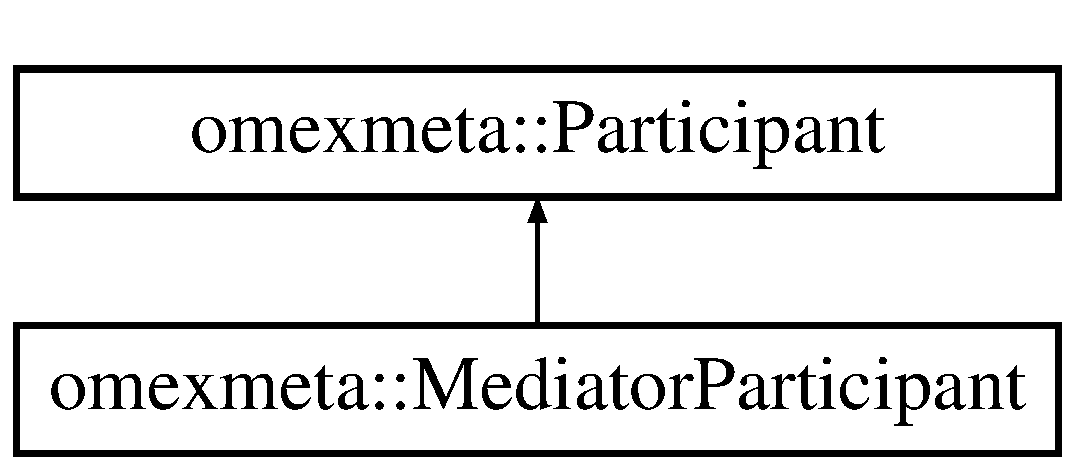
\includegraphics[height=2.000000cm]{classomexmeta_1_1MediatorParticipant}
\end{center}
\end{figure}
\doxysubsection*{Public Member Functions}
\begin{DoxyCompactItemize}
\item 
\mbox{\Hypertarget{classomexmeta_1_1MediatorParticipant_a14ff63de2df15706051787f7445d1fec}\label{classomexmeta_1_1MediatorParticipant_a14ff63de2df15706051787f7445d1fec}} 
\mbox{\hyperlink{classomexmeta_1_1MediatorParticipant_a14ff63de2df15706051787f7445d1fec}{Mediator\+Participant}} (librdf\+\_\+model $\ast$model, std\+::string physical\+Entity\+Reference, e\+Uri\+Type type, \mbox{\hyperlink{classomexmeta_1_1UriHandler}{Uri\+Handler}} \&uri\+Handler)
\begin{DoxyCompactList}\small\item\em A class representing process mediators (such as a catalyst). \end{DoxyCompactList}\end{DoxyCompactItemize}


\doxysubsection{Detailed Description}
\mbox{\hyperlink{classSubclass}{Subclass}} of \mbox{\hyperlink{classomexmeta_1_1Participant}{Participant}}. See Participants for arguments. 

The documentation for this class was generated from the following files\+:\begin{DoxyCompactItemize}
\item 
src/omexmeta/include/omexmeta/Participant.\+h\item 
src/omexmeta/Participant.\+cpp\end{DoxyCompactItemize}

\hypertarget{classomexmeta_1_1MetaID}{}\section{omexmeta\+:\+:Meta\+ID Class Reference}
\label{classomexmeta_1_1MetaID}\index{omexmeta\+::\+Meta\+ID@{omexmeta\+::\+Meta\+ID}}


an ID generator  




{\ttfamily \#include $<$Meta\+I\+D.\+h$>$}

\subsection*{Public Member Functions}
\begin{DoxyCompactItemize}
\item 
\hyperlink{classomexmeta_1_1MetaID_af5cc076ccd6db8c411de98902d2a1218}{Meta\+ID} (std\+::string base, long start\+\_\+number, int num\+\_\+digits=4)
\begin{DoxyCompactList}\small\item\em an ID generator used when creating I\+Ds in the \hyperlink{classomexmeta_1_1Editor}{Editor}. \end{DoxyCompactList}\item 
\mbox{\Hypertarget{classomexmeta_1_1MetaID_a3d6466efca8d9e931ca8c440c0809584}\label{classomexmeta_1_1MetaID_a3d6466efca8d9e931ca8c440c0809584}} 
bool {\bfseries operator==} (const \hyperlink{classomexmeta_1_1MetaID}{Meta\+ID} \&rhs) const
\item 
\mbox{\Hypertarget{classomexmeta_1_1MetaID_a25af693b284b0110914c537b48b20937}\label{classomexmeta_1_1MetaID_a25af693b284b0110914c537b48b20937}} 
bool {\bfseries operator!=} (const \hyperlink{classomexmeta_1_1MetaID}{Meta\+ID} \&rhs) const
\item 
std\+::string \hyperlink{classomexmeta_1_1MetaID_a95e709df9b0ee47473bc40012738cdc8}{generate} () const
\begin{DoxyCompactList}\small\item\em generate the string for a metaid \end{DoxyCompactList}\item 
std\+::string \hyperlink{classomexmeta_1_1MetaID_a9a3c9b479d522e7630275d85582edd26}{generate} (long n) const
\begin{DoxyCompactList}\small\item\em generate the string for a metaid \end{DoxyCompactList}\item 
int \hyperlink{classomexmeta_1_1MetaID_a343f4b48c9673f8943e03057370f01e4}{max\+Number} () const
\begin{DoxyCompactList}\small\item\em figure out the max number possible with user parameters \end{DoxyCompactList}\end{DoxyCompactItemize}
\subsection*{Static Public Member Functions}
\begin{DoxyCompactItemize}
\item 
static int \hyperlink{classomexmeta_1_1MetaID_ae4fe83a3512f64065e8e2997bc710be6}{count\+Digits} (long long int n)
\begin{DoxyCompactList}\small\item\em count the digits in a number \end{DoxyCompactList}\end{DoxyCompactItemize}


\subsection{Detailed Description}
an ID generator 

\subsection{Constructor \& Destructor Documentation}
\mbox{\Hypertarget{classomexmeta_1_1MetaID_af5cc076ccd6db8c411de98902d2a1218}\label{classomexmeta_1_1MetaID_af5cc076ccd6db8c411de98902d2a1218}} 
\index{omexmeta\+::\+Meta\+ID@{omexmeta\+::\+Meta\+ID}!Meta\+ID@{Meta\+ID}}
\index{Meta\+ID@{Meta\+ID}!omexmeta\+::\+Meta\+ID@{omexmeta\+::\+Meta\+ID}}
\subsubsection{\texorpdfstring{Meta\+I\+D()}{MetaID()}}
{\footnotesize\ttfamily omexmeta\+::\+Meta\+I\+D\+::\+Meta\+ID (\begin{DoxyParamCaption}\item[{std\+::string}]{base,  }\item[{long}]{start\+\_\+number,  }\item[{int}]{num\+\_\+digits = {\ttfamily 4} }\end{DoxyParamCaption})}



an ID generator used when creating I\+Ds in the \hyperlink{classomexmeta_1_1Editor}{Editor}. 


\begin{DoxyParams}{Parameters}
{\em base\+\_\+} & the constant portion of the id. Like semsim in semsim00001 \\
\hline
{\em start\+\_\+number\+\_\+} & the start\+\_\+number portion of the id, like 1 in semsim00001 \\
\hline
{\em num\+\_\+digits} & specifies the start\+\_\+number of digits to use in the id. So semsim00001 has 5 digits.\\
\hline
\end{DoxyParams}


\hyperlink{classomexmeta_1_1MetaID}{Meta\+ID} metaid(\char`\"{}\+A\+New\+Meta\+I\+D\char`\"{}, 15, 3); std\+::string id = metaid.\+generate(); 

\subsection{Member Function Documentation}
\mbox{\Hypertarget{classomexmeta_1_1MetaID_ae4fe83a3512f64065e8e2997bc710be6}\label{classomexmeta_1_1MetaID_ae4fe83a3512f64065e8e2997bc710be6}} 
\index{omexmeta\+::\+Meta\+ID@{omexmeta\+::\+Meta\+ID}!count\+Digits@{count\+Digits}}
\index{count\+Digits@{count\+Digits}!omexmeta\+::\+Meta\+ID@{omexmeta\+::\+Meta\+ID}}
\subsubsection{\texorpdfstring{count\+Digits()}{countDigits()}}
{\footnotesize\ttfamily int omexmeta\+::\+Meta\+I\+D\+::count\+Digits (\begin{DoxyParamCaption}\item[{long long int}]{n }\end{DoxyParamCaption})\hspace{0.3cm}{\ttfamily [static]}}



count the digits in a number 


\begin{DoxyParams}{Parameters}
{\em n} & the number to count digits in \\
\hline
\end{DoxyParams}
\begin{DoxyReturn}{Returns}
the number of digits in n 
\end{DoxyReturn}
\mbox{\Hypertarget{classomexmeta_1_1MetaID_a95e709df9b0ee47473bc40012738cdc8}\label{classomexmeta_1_1MetaID_a95e709df9b0ee47473bc40012738cdc8}} 
\index{omexmeta\+::\+Meta\+ID@{omexmeta\+::\+Meta\+ID}!generate@{generate}}
\index{generate@{generate}!omexmeta\+::\+Meta\+ID@{omexmeta\+::\+Meta\+ID}}
\subsubsection{\texorpdfstring{generate()}{generate()}\hspace{0.1cm}{\footnotesize\ttfamily [1/2]}}
{\footnotesize\ttfamily std\+::string omexmeta\+::\+Meta\+I\+D\+::generate (\begin{DoxyParamCaption}{ }\end{DoxyParamCaption}) const}



generate the string for a metaid 

\begin{DoxyReturn}{Returns}
a metaid defined by the parameters in instantiation 
\end{DoxyReturn}
\mbox{\Hypertarget{classomexmeta_1_1MetaID_a9a3c9b479d522e7630275d85582edd26}\label{classomexmeta_1_1MetaID_a9a3c9b479d522e7630275d85582edd26}} 
\index{omexmeta\+::\+Meta\+ID@{omexmeta\+::\+Meta\+ID}!generate@{generate}}
\index{generate@{generate}!omexmeta\+::\+Meta\+ID@{omexmeta\+::\+Meta\+ID}}
\subsubsection{\texorpdfstring{generate()}{generate()}\hspace{0.1cm}{\footnotesize\ttfamily [2/2]}}
{\footnotesize\ttfamily std\+::string omexmeta\+::\+Meta\+I\+D\+::generate (\begin{DoxyParamCaption}\item[{long}]{n }\end{DoxyParamCaption}) const}



generate the string for a metaid 


\begin{DoxyParams}{Parameters}
{\em number} & of digits \\
\hline
\end{DoxyParams}
\begin{DoxyReturn}{Returns}
a metaid defined by the parameters in instantiation 
\end{DoxyReturn}
\mbox{\Hypertarget{classomexmeta_1_1MetaID_a343f4b48c9673f8943e03057370f01e4}\label{classomexmeta_1_1MetaID_a343f4b48c9673f8943e03057370f01e4}} 
\index{omexmeta\+::\+Meta\+ID@{omexmeta\+::\+Meta\+ID}!max\+Number@{max\+Number}}
\index{max\+Number@{max\+Number}!omexmeta\+::\+Meta\+ID@{omexmeta\+::\+Meta\+ID}}
\subsubsection{\texorpdfstring{max\+Number()}{maxNumber()}}
{\footnotesize\ttfamily int omexmeta\+::\+Meta\+I\+D\+::max\+Number (\begin{DoxyParamCaption}{ }\end{DoxyParamCaption}) const}



figure out the max number possible with user parameters 

\begin{DoxyReturn}{Returns}
the maximum possible number with user parameters 
\end{DoxyReturn}


The documentation for this class was generated from the following files\+:\begin{DoxyCompactItemize}
\item 
src/omexmeta/Meta\+I\+D.\+h\item 
src/omexmeta/Meta\+I\+D.\+cpp\end{DoxyCompactItemize}

\hypertarget{structNone}{}\doxysection{None Struct Reference}
\label{structNone}\index{None@{None}}


The documentation for this struct was generated from the following file\+:\begin{DoxyCompactItemize}
\item 
src/omexmeta/logger.\+h\end{DoxyCompactItemize}

\hypertarget{structdbg_1_1detail__detector_1_1nonesuch}{}\doxysection{dbg\+::detail\+\_\+detector\+::nonesuch Struct Reference}
\label{structdbg_1_1detail__detector_1_1nonesuch}\index{dbg::detail\_detector::nonesuch@{dbg::detail\_detector::nonesuch}}
\doxysubsection*{Public Member Functions}
\begin{DoxyCompactItemize}
\item 
\mbox{\Hypertarget{structdbg_1_1detail__detector_1_1nonesuch_a82c9bfc90b56b542819d8df5af7cebe6}\label{structdbg_1_1detail__detector_1_1nonesuch_a82c9bfc90b56b542819d8df5af7cebe6}} 
{\bfseries nonesuch} (\mbox{\hyperlink{structdbg_1_1detail__detector_1_1nonesuch}{nonesuch}} const \&)=delete
\item 
\mbox{\Hypertarget{structdbg_1_1detail__detector_1_1nonesuch_af0d1b2ab32ace678e2c9d95684d1917b}\label{structdbg_1_1detail__detector_1_1nonesuch_af0d1b2ab32ace678e2c9d95684d1917b}} 
void {\bfseries operator=} (\mbox{\hyperlink{structdbg_1_1detail__detector_1_1nonesuch}{nonesuch}} const \&)=delete
\end{DoxyCompactItemize}


The documentation for this struct was generated from the following file\+:\begin{DoxyCompactItemize}
\item 
src/omexmeta/include/omexmeta/dbg.\+h\end{DoxyCompactItemize}

\hypertarget{classomexmeta_1_1NotImplementedException}{}\section{omexmeta\+:\+:Not\+Implemented\+Exception Class Reference}
\label{classomexmeta_1_1NotImplementedException}\index{omexmeta\+::\+Not\+Implemented\+Exception@{omexmeta\+::\+Not\+Implemented\+Exception}}
Inheritance diagram for omexmeta\+:\+:Not\+Implemented\+Exception\+:\begin{figure}[H]
\begin{center}
\leavevmode
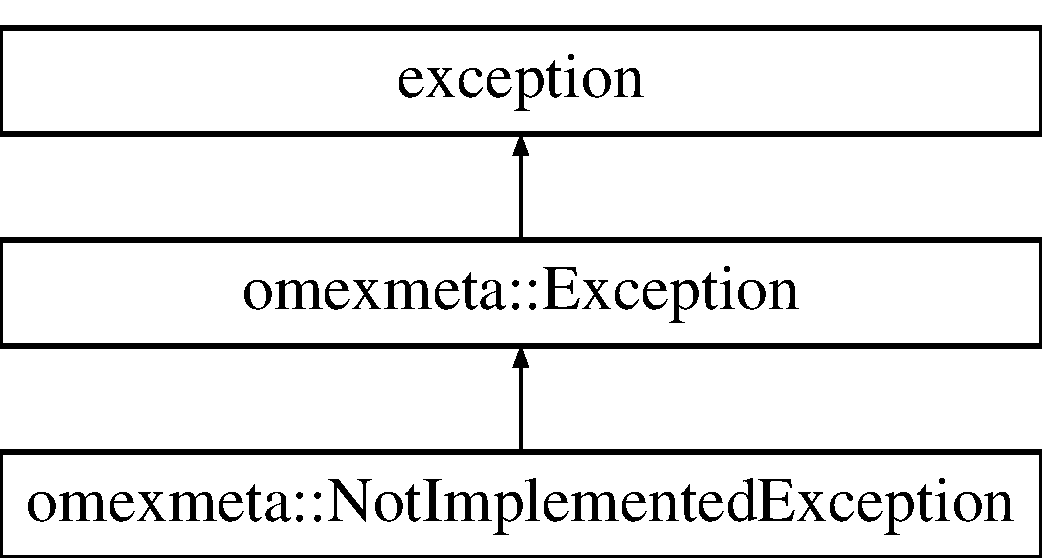
\includegraphics[height=3.000000cm]{classomexmeta_1_1NotImplementedException}
\end{center}
\end{figure}
\subsection*{Additional Inherited Members}


The documentation for this class was generated from the following file\+:\begin{DoxyCompactItemize}
\item 
src/omexmeta/Error.\+h\end{DoxyCompactItemize}

\hypertarget{classomexmeta_1_1NullPointerException}{}\doxysection{omexmeta\+::Null\+Pointer\+Exception Class Reference}
\label{classomexmeta_1_1NullPointerException}\index{omexmeta::NullPointerException@{omexmeta::NullPointerException}}
Inheritance diagram for omexmeta\+::Null\+Pointer\+Exception\+:\begin{figure}[H]
\begin{center}
\leavevmode
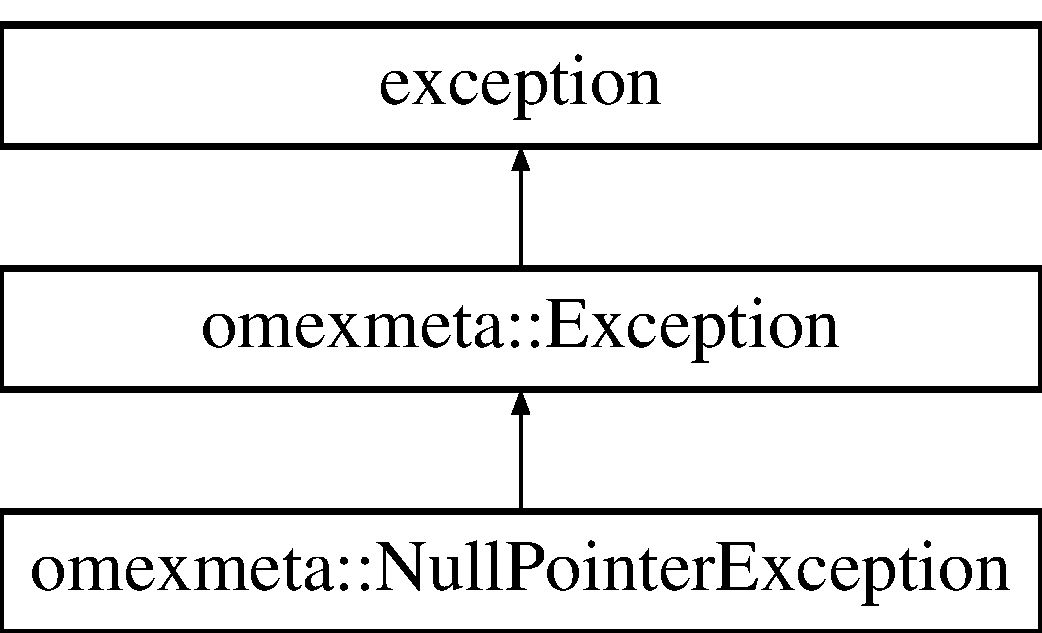
\includegraphics[height=3.000000cm]{classomexmeta_1_1NullPointerException}
\end{center}
\end{figure}
\doxysubsection*{Additional Inherited Members}


The documentation for this class was generated from the following file\+:\begin{DoxyCompactItemize}
\item 
src/omexmeta/include/omexmeta/Error.\+h\end{DoxyCompactItemize}

\hypertarget{classomexmeta_1_1OmexMetaUtils}{}\doxysection{omexmeta\+::Omex\+Meta\+Utils Class Reference}
\label{classomexmeta_1_1OmexMetaUtils}\index{omexmeta::OmexMetaUtils@{omexmeta::OmexMetaUtils}}
\doxysubsection*{Static Public Member Functions}
\begin{DoxyCompactItemize}
\item 
static bool \mbox{\hyperlink{classomexmeta_1_1OmexMetaUtils_ab72b362607e6bbdd0025eefa574cd073}{exists}} (const std\+::string \&filename)
\begin{DoxyCompactList}\small\item\em return true when filename is a file that exists on system \end{DoxyCompactList}\item 
static int \mbox{\hyperlink{classomexmeta_1_1OmexMetaUtils_a9c445a8e0cc6589b25d6fa630686c171}{remove\+File}} (const std\+::string \&filename)
\begin{DoxyCompactList}\small\item\em remove file called \end{DoxyCompactList}\item 
static void \mbox{\hyperlink{classomexmeta_1_1OmexMetaUtils_a8e629136cb2685ed839ea3a0e88094e6}{remove\+If\+Exists}} (const std\+::string \&filename)
\begin{DoxyCompactList}\small\item\em remove a file, checking for its existance first \end{DoxyCompactList}\item 
static void \mbox{\hyperlink{classomexmeta_1_1OmexMetaUtils_a046b603d6308242b70b55de6cb72325c}{download}} (const std\+::string \&url, std\+::string filename)
\begin{DoxyCompactList}\small\item\em download a file from \end{DoxyCompactList}\item 
static std\+::vector$<$ std\+::string $>$ \mbox{\hyperlink{classomexmeta_1_1OmexMetaUtils_aac769ce6e901f32820cd7dc3fef989fa}{split\+String\+By}} (const std\+::string \&str, char delimiter)
\begin{DoxyCompactList}\small\item\em split a string into a vector of strings by \end{DoxyCompactList}\item 
static std\+::string \mbox{\hyperlink{classomexmeta_1_1OmexMetaUtils_a4700231d455a5f65f7cc290d98d2b0ec}{generate\+Unique\+Metaid}} (librdf\+\_\+model $\ast$model, const std\+::string \&metaid\+\_\+base, std\+::vector$<$ std\+::string $>$ \&exclusions)
\begin{DoxyCompactList}\small\item\em utility for generating unique metaids given an xml document \end{DoxyCompactList}\item 
static std\+::string \mbox{\hyperlink{classomexmeta_1_1OmexMetaUtils_a6694715cf3f5dccd33d416ecc84ff375}{prepare\+Base\+Uri}} (std\+::string str, bool absolute\+\_\+path=false)
\begin{DoxyCompactList}\small\item\em process a string intended to be a base uri. \end{DoxyCompactList}\item 
static std\+::string \mbox{\hyperlink{classomexmeta_1_1OmexMetaUtils_a0956bde073b212596d8e4b2ffc983e47}{get\+Namespace\+From\+Uri}} (const std\+::string \&uri)
\begin{DoxyCompactList}\small\item\em takes a uri as std\+::string and returns the string with the last section removed; \end{DoxyCompactList}\item 
static bool \mbox{\hyperlink{classomexmeta_1_1OmexMetaUtils_af663724f2efb0324a64c6a57e8491c13}{is\+Formatted\+Uri}} (std\+::string uri)
\begin{DoxyCompactList}\small\item\em helper function that returns true when uri starts with either {\ttfamily \href{https://}{\texttt{ https\+://}}} {\ttfamily \href{http://}{\texttt{ http\+://}}} or {\ttfamily \href{file://}{\texttt{ file\+://}}} \end{DoxyCompactList}\item 
static bool \mbox{\hyperlink{classomexmeta_1_1OmexMetaUtils_a9c2b712b85f74fff9740477660f7b371}{ends\+With}} (std\+::string const \&full\+\_\+string, std\+::string const \&ending)
\begin{DoxyCompactList}\small\item\em test to see whether a string ends with another string \end{DoxyCompactList}\item 
\mbox{\Hypertarget{classomexmeta_1_1OmexMetaUtils_a4ec81c80bf33d232331ea9ef0b94da61}\label{classomexmeta_1_1OmexMetaUtils_a4ec81c80bf33d232331ea9ef0b94da61}} 
static bool \mbox{\hyperlink{classomexmeta_1_1OmexMetaUtils_a4ec81c80bf33d232331ea9ef0b94da61}{assert\+Regex\+Match\+Split\+By\+New\+Line}} (const std\+::string \&expected\+\_\+string, const std\+::string \&actual\+\_\+string)
\begin{DoxyCompactList}\small\item\em test that expected\+\_\+string matches actual\+\_\+string when split by new lines and matched as a regex \end{DoxyCompactList}\item 
\mbox{\Hypertarget{classomexmeta_1_1OmexMetaUtils_a6ddc16d56f238ef7ff3c8ab355163ef7}\label{classomexmeta_1_1OmexMetaUtils_a6ddc16d56f238ef7ff3c8ab355163ef7}} 
static bool {\bfseries assert\+Match\+By\+New\+Line} (const std\+::string \&expected\+\_\+string, const std\+::string \&actual\+\_\+string)
\item 
static std\+::vector$<$ std\+::string $>$ \mbox{\hyperlink{classomexmeta_1_1OmexMetaUtils_a744a0575136f1cc60b76a6560a5595e9}{configure\+Prefix\+Strings}} (std\+::string repository\+\_\+name, std\+::string omex\+\_\+name, std\+::string model\+\_\+name)
\begin{DoxyCompactList}\small\item\em configures the \char`\"{}\+O\+M\+E\+Xlib\char`\"{}, \char`\"{}my\+O\+M\+E\+X\char`\"{} and \char`\"{}local\char`\"{} prefixes @ param omex\+\_\+name the name of the omex container your model is in \end{DoxyCompactList}\item 
static std\+::string \mbox{\hyperlink{classomexmeta_1_1OmexMetaUtils_ae645af49ce57dac8bd0e0eba9e39a6c0}{concat\+Meta\+Id\+And\+Uri}} (std\+::string metaid, std\+::string uri)
\begin{DoxyCompactList}\small\item\em concatonate metaid and uri strings \end{DoxyCompactList}\item 
static std\+::string \mbox{\hyperlink{classomexmeta_1_1OmexMetaUtils_aca2230ca99338b9dc0fc7d296b0c553b}{string\+Replace}} (std\+::string str, const std\+::string \&string\+\_\+to\+\_\+replace, const std\+::string \&replacement)
\begin{DoxyCompactList}\small\item\em replace a part of a string @string\+\_\+to\+\_\+replace from a main \end{DoxyCompactList}\item 
static bool \mbox{\hyperlink{classomexmeta_1_1OmexMetaUtils_a66d58e0ebcbee1857b23ead70c87de7f}{starts\+With}} (const std\+::string \&full\+\_\+string, const std\+::string \&start)
\begin{DoxyCompactList}\small\item\em returns true when \end{DoxyCompactList}\item 
static bool \mbox{\hyperlink{classomexmeta_1_1OmexMetaUtils_a6f8e406b8798bd2f1f0ae0d1bd07ed2b}{string\+In\+Vector}} (std\+::vector$<$ std\+::string $>$ vec, const std\+::string \&string)
\begin{DoxyCompactList}\small\item\em returns true when \end{DoxyCompactList}\item 
static xml\+Doc $\ast$ \mbox{\hyperlink{classomexmeta_1_1OmexMetaUtils_a718710d8ba7fc7598bd73a5456b3d903}{parse\+Xml\+Document}} (const std\+::string \&xml\+\_\+string)
\begin{DoxyCompactList}\small\item\em read an xml document using libxml2. \end{DoxyCompactList}\item 
\mbox{\Hypertarget{classomexmeta_1_1OmexMetaUtils_a29cc8222c809162eadbc424a0687cbf3}\label{classomexmeta_1_1OmexMetaUtils_a29cc8222c809162eadbc424a0687cbf3}} 
static std\+::string {\bfseries get\+Xml\+Node\+Property} (xml\+Node $\ast$node, const std\+::string \&property)
\item 
\mbox{\Hypertarget{classomexmeta_1_1OmexMetaUtils_a1dbcd874b2b72531e7f4f9e82524d8e8}\label{classomexmeta_1_1OmexMetaUtils_a1dbcd874b2b72531e7f4f9e82524d8e8}} 
static xml\+Node $\ast$ {\bfseries get\+Child\+Element\+Called} (xml\+Node $\ast$node, const std\+::string \&name)
\item 
\mbox{\Hypertarget{classomexmeta_1_1OmexMetaUtils_a4d6f7d2140c42435be9339edf975b949}\label{classomexmeta_1_1OmexMetaUtils_a4d6f7d2140c42435be9339edf975b949}} 
static std\+::vector$<$ xml\+Node $\ast$ $>$ {\bfseries get\+All\+Child\+Elements} (xml\+Node $\ast$node)
\item 
\mbox{\Hypertarget{classomexmeta_1_1OmexMetaUtils_a96e93667c8799b9569cb30fc102b129b}\label{classomexmeta_1_1OmexMetaUtils_a96e93667c8799b9569cb30fc102b129b}} 
static bool {\bfseries is\+Sub\+String} (const std\+::string \&full\+\_\+string, const std\+::string \&substring)
\end{DoxyCompactItemize}


\doxysubsection{Member Function Documentation}
\mbox{\Hypertarget{classomexmeta_1_1OmexMetaUtils_ae645af49ce57dac8bd0e0eba9e39a6c0}\label{classomexmeta_1_1OmexMetaUtils_ae645af49ce57dac8bd0e0eba9e39a6c0}} 
\index{omexmeta::OmexMetaUtils@{omexmeta::OmexMetaUtils}!concatMetaIdAndUri@{concatMetaIdAndUri}}
\index{concatMetaIdAndUri@{concatMetaIdAndUri}!omexmeta::OmexMetaUtils@{omexmeta::OmexMetaUtils}}
\doxysubsubsection{\texorpdfstring{concatMetaIdAndUri()}{concatMetaIdAndUri()}}
{\footnotesize\ttfamily std\+::string omexmeta\+::\+Omex\+Meta\+Utils\+::concat\+Meta\+Id\+And\+Uri (\begin{DoxyParamCaption}\item[{std\+::string}]{metaid,  }\item[{std\+::string}]{uri }\end{DoxyParamCaption})\hspace{0.3cm}{\ttfamily [static]}}



concatonate metaid and uri strings 


\begin{DoxyParams}{Parameters}
{\em metaid} & string. Like \char`\"{}\#metaid\char`\"{} or \char`\"{}metaid\char`\"{} \\
\hline
{\em uri} & string. Like \char`\"{}https\+://omex-\/library/jeff2019.\+omex/mymodel.\+xml\char`\"{} or \char`\"{}https\+://omex-\/library/jeff2019.\+omex/mymodel.\+rdf\char`\"{}  Sometimes a uri has a trailing \char`\"{}\#\char`\"{} and somtimes a metaid has a leading \char`\"{}\#\char`\"{}. \mbox{\hyperlink{classThis}{This}} method concatonates whilst accounting for permutations of \char`\"{}\#\char`\"{} \\
\hline
\end{DoxyParams}
\mbox{\Hypertarget{classomexmeta_1_1OmexMetaUtils_a744a0575136f1cc60b76a6560a5595e9}\label{classomexmeta_1_1OmexMetaUtils_a744a0575136f1cc60b76a6560a5595e9}} 
\index{omexmeta::OmexMetaUtils@{omexmeta::OmexMetaUtils}!configurePrefixStrings@{configurePrefixStrings}}
\index{configurePrefixStrings@{configurePrefixStrings}!omexmeta::OmexMetaUtils@{omexmeta::OmexMetaUtils}}
\doxysubsubsection{\texorpdfstring{configurePrefixStrings()}{configurePrefixStrings()}}
{\footnotesize\ttfamily std\+::vector$<$ std\+::string $>$ omexmeta\+::\+Omex\+Meta\+Utils\+::configure\+Prefix\+Strings (\begin{DoxyParamCaption}\item[{std\+::string}]{repository\+\_\+name,  }\item[{std\+::string}]{omex\+\_\+name,  }\item[{std\+::string}]{model\+\_\+name }\end{DoxyParamCaption})\hspace{0.3cm}{\ttfamily [static]}}



configures the \char`\"{}\+O\+M\+E\+Xlib\char`\"{}, \char`\"{}my\+O\+M\+E\+X\char`\"{} and \char`\"{}local\char`\"{} prefixes @ param omex\+\_\+name the name of the omex container your model is in 


\begin{DoxyParams}{Parameters}
{\em model\+\_\+name} & the name of the model your are annotating. Extension should be included or it will be given the \char`\"{}.\+xml\char`\"{} suffix. \\
\hline
\end{DoxyParams}
\mbox{\Hypertarget{classomexmeta_1_1OmexMetaUtils_a046b603d6308242b70b55de6cb72325c}\label{classomexmeta_1_1OmexMetaUtils_a046b603d6308242b70b55de6cb72325c}} 
\index{omexmeta::OmexMetaUtils@{omexmeta::OmexMetaUtils}!download@{download}}
\index{download@{download}!omexmeta::OmexMetaUtils@{omexmeta::OmexMetaUtils}}
\doxysubsubsection{\texorpdfstring{download()}{download()}}
{\footnotesize\ttfamily void omexmeta\+::\+Omex\+Meta\+Utils\+::download (\begin{DoxyParamCaption}\item[{const std\+::string \&}]{url,  }\item[{std\+::string}]{filename }\end{DoxyParamCaption})\hspace{0.3cm}{\ttfamily [static]}}



download a file from 


\begin{DoxyParams}{Parameters}
{\em url} & to\\
\hline
{\em filename} & \begin{DoxyVerb}wrapper around the CurlGet function, as the utils
\end{DoxyVerb}
 class seems like a good place for the download features. \\
\hline
\end{DoxyParams}
\mbox{\Hypertarget{classomexmeta_1_1OmexMetaUtils_a9c2b712b85f74fff9740477660f7b371}\label{classomexmeta_1_1OmexMetaUtils_a9c2b712b85f74fff9740477660f7b371}} 
\index{omexmeta::OmexMetaUtils@{omexmeta::OmexMetaUtils}!endsWith@{endsWith}}
\index{endsWith@{endsWith}!omexmeta::OmexMetaUtils@{omexmeta::OmexMetaUtils}}
\doxysubsubsection{\texorpdfstring{endsWith()}{endsWith()}}
{\footnotesize\ttfamily bool omexmeta\+::\+Omex\+Meta\+Utils\+::ends\+With (\begin{DoxyParamCaption}\item[{std\+::string const \&}]{full\+\_\+string,  }\item[{std\+::string const \&}]{ending }\end{DoxyParamCaption})\hspace{0.3cm}{\ttfamily [static]}}



test to see whether a string ends with another string 


\begin{DoxyParams}{Parameters}
{\em full\+String} & the string to test \\
\hline
{\em ending} & the ending to test for \\
\hline
\end{DoxyParams}
\mbox{\Hypertarget{classomexmeta_1_1OmexMetaUtils_ab72b362607e6bbdd0025eefa574cd073}\label{classomexmeta_1_1OmexMetaUtils_ab72b362607e6bbdd0025eefa574cd073}} 
\index{omexmeta::OmexMetaUtils@{omexmeta::OmexMetaUtils}!exists@{exists}}
\index{exists@{exists}!omexmeta::OmexMetaUtils@{omexmeta::OmexMetaUtils}}
\doxysubsubsection{\texorpdfstring{exists()}{exists()}}
{\footnotesize\ttfamily bool omexmeta\+::\+Omex\+Meta\+Utils\+::exists (\begin{DoxyParamCaption}\item[{const std\+::string \&}]{filename }\end{DoxyParamCaption})\hspace{0.3cm}{\ttfamily [static]}}



return true when filename is a file that exists on system 


\begin{DoxyParams}{Parameters}
{\em filename} & \\
\hline
\end{DoxyParams}
\mbox{\Hypertarget{classomexmeta_1_1OmexMetaUtils_a4700231d455a5f65f7cc290d98d2b0ec}\label{classomexmeta_1_1OmexMetaUtils_a4700231d455a5f65f7cc290d98d2b0ec}} 
\index{omexmeta::OmexMetaUtils@{omexmeta::OmexMetaUtils}!generateUniqueMetaid@{generateUniqueMetaid}}
\index{generateUniqueMetaid@{generateUniqueMetaid}!omexmeta::OmexMetaUtils@{omexmeta::OmexMetaUtils}}
\doxysubsubsection{\texorpdfstring{generateUniqueMetaid()}{generateUniqueMetaid()}}
{\footnotesize\ttfamily std\+::string omexmeta\+::\+Omex\+Meta\+Utils\+::generate\+Unique\+Metaid (\begin{DoxyParamCaption}\item[{librdf\+\_\+model $\ast$}]{model,  }\item[{const std\+::string \&}]{metaid\+\_\+base,  }\item[{std\+::vector$<$ std\+::string $>$ \&}]{exclusions }\end{DoxyParamCaption})\hspace{0.3cm}{\ttfamily [static]}}



utility for generating unique metaids given an xml document 

model a librdf\+\_\+model$\ast$ pointer

a string that will be used for the ID. There will be 4 digits, though this can be changed.

exclusions. Mostly needed internally for dealing with metaids that already exist. \mbox{\Hypertarget{classomexmeta_1_1OmexMetaUtils_a0956bde073b212596d8e4b2ffc983e47}\label{classomexmeta_1_1OmexMetaUtils_a0956bde073b212596d8e4b2ffc983e47}} 
\index{omexmeta::OmexMetaUtils@{omexmeta::OmexMetaUtils}!getNamespaceFromUri@{getNamespaceFromUri}}
\index{getNamespaceFromUri@{getNamespaceFromUri}!omexmeta::OmexMetaUtils@{omexmeta::OmexMetaUtils}}
\doxysubsubsection{\texorpdfstring{getNamespaceFromUri()}{getNamespaceFromUri()}}
{\footnotesize\ttfamily std\+::string omexmeta\+::\+Omex\+Meta\+Utils\+::get\+Namespace\+From\+Uri (\begin{DoxyParamCaption}\item[{const std\+::string \&}]{uri }\end{DoxyParamCaption})\hspace{0.3cm}{\ttfamily [static]}}



takes a uri as std\+::string and returns the string with the last section removed; 

Example\+: www.\+uri.\+com/identifer/\+P\+D12345 will turn into www.\+uri.\+com/identifier/ \mbox{\Hypertarget{classomexmeta_1_1OmexMetaUtils_af663724f2efb0324a64c6a57e8491c13}\label{classomexmeta_1_1OmexMetaUtils_af663724f2efb0324a64c6a57e8491c13}} 
\index{omexmeta::OmexMetaUtils@{omexmeta::OmexMetaUtils}!isFormattedUri@{isFormattedUri}}
\index{isFormattedUri@{isFormattedUri}!omexmeta::OmexMetaUtils@{omexmeta::OmexMetaUtils}}
\doxysubsubsection{\texorpdfstring{isFormattedUri()}{isFormattedUri()}}
{\footnotesize\ttfamily bool omexmeta\+::\+Omex\+Meta\+Utils\+::is\+Formatted\+Uri (\begin{DoxyParamCaption}\item[{std\+::string}]{uri }\end{DoxyParamCaption})\hspace{0.3cm}{\ttfamily [static]}}



helper function that returns true when uri starts with either {\ttfamily \href{https://}{\texttt{ https\+://}}} {\ttfamily \href{http://}{\texttt{ http\+://}}} or {\ttfamily \href{file://}{\texttt{ file\+://}}} 


\begin{DoxyParams}{Parameters}
{\em uri} & the uri to test. \\
\hline
\end{DoxyParams}
\mbox{\Hypertarget{classomexmeta_1_1OmexMetaUtils_a718710d8ba7fc7598bd73a5456b3d903}\label{classomexmeta_1_1OmexMetaUtils_a718710d8ba7fc7598bd73a5456b3d903}} 
\index{omexmeta::OmexMetaUtils@{omexmeta::OmexMetaUtils}!parseXmlDocument@{parseXmlDocument}}
\index{parseXmlDocument@{parseXmlDocument}!omexmeta::OmexMetaUtils@{omexmeta::OmexMetaUtils}}
\doxysubsubsection{\texorpdfstring{parseXmlDocument()}{parseXmlDocument()}}
{\footnotesize\ttfamily xml\+Doc $\ast$ omexmeta\+::\+Omex\+Meta\+Utils\+::parse\+Xml\+Document (\begin{DoxyParamCaption}\item[{const std\+::string \&}]{xml\+\_\+string }\end{DoxyParamCaption})\hspace{0.3cm}{\ttfamily [static]}}



read an xml document using libxml2. 

\begin{DoxyReturn}{Returns}
xml\+Doc$\ast$. Caller is responsible for calling xml\+Free\+Doc(doc). 
\end{DoxyReturn}
\mbox{\Hypertarget{classomexmeta_1_1OmexMetaUtils_a6694715cf3f5dccd33d416ecc84ff375}\label{classomexmeta_1_1OmexMetaUtils_a6694715cf3f5dccd33d416ecc84ff375}} 
\index{omexmeta::OmexMetaUtils@{omexmeta::OmexMetaUtils}!prepareBaseUri@{prepareBaseUri}}
\index{prepareBaseUri@{prepareBaseUri}!omexmeta::OmexMetaUtils@{omexmeta::OmexMetaUtils}}
\doxysubsubsection{\texorpdfstring{prepareBaseUri()}{prepareBaseUri()}}
{\footnotesize\ttfamily std\+::string omexmeta\+::\+Omex\+Meta\+Utils\+::prepare\+Base\+Uri (\begin{DoxyParamCaption}\item[{std\+::string}]{str,  }\item[{bool}]{absolute\+\_\+path = {\ttfamily false} }\end{DoxyParamCaption})\hspace{0.3cm}{\ttfamily [static]}}



process a string intended to be a base uri. 


\begin{DoxyParams}{Parameters}
{\em str} & The string that will become a base uri \\
\hline
{\em absolute\+\_\+path} & automatically make str an absolute path to the current working directory.\\
\hline
\end{DoxyParams}
Base uri\textquotesingle{}s are important in redland libraries. If they do not begin with {\ttfamily \href{file://}{\texttt{ file\+://}}} {\ttfamily http} or {\ttfamily https}, sparql querying will break down. \mbox{\hyperlink{classThis}{This}} is a helper function to ensure the base uri is properly formatted. \mbox{\Hypertarget{classomexmeta_1_1OmexMetaUtils_a9c445a8e0cc6589b25d6fa630686c171}\label{classomexmeta_1_1OmexMetaUtils_a9c445a8e0cc6589b25d6fa630686c171}} 
\index{omexmeta::OmexMetaUtils@{omexmeta::OmexMetaUtils}!removeFile@{removeFile}}
\index{removeFile@{removeFile}!omexmeta::OmexMetaUtils@{omexmeta::OmexMetaUtils}}
\doxysubsubsection{\texorpdfstring{removeFile()}{removeFile()}}
{\footnotesize\ttfamily int omexmeta\+::\+Omex\+Meta\+Utils\+::remove\+File (\begin{DoxyParamCaption}\item[{const std\+::string \&}]{filename }\end{DoxyParamCaption})\hspace{0.3cm}{\ttfamily [static]}}



remove file called 


\begin{DoxyParams}{Parameters}
{\em filename} & \\
\hline
{\em filename} & to remove \\
\hline
\end{DoxyParams}
\begin{DoxyReturn}{Returns}
int 0 when successful. 
\end{DoxyReturn}
\mbox{\Hypertarget{classomexmeta_1_1OmexMetaUtils_a8e629136cb2685ed839ea3a0e88094e6}\label{classomexmeta_1_1OmexMetaUtils_a8e629136cb2685ed839ea3a0e88094e6}} 
\index{omexmeta::OmexMetaUtils@{omexmeta::OmexMetaUtils}!removeIfExists@{removeIfExists}}
\index{removeIfExists@{removeIfExists}!omexmeta::OmexMetaUtils@{omexmeta::OmexMetaUtils}}
\doxysubsubsection{\texorpdfstring{removeIfExists()}{removeIfExists()}}
{\footnotesize\ttfamily void omexmeta\+::\+Omex\+Meta\+Utils\+::remove\+If\+Exists (\begin{DoxyParamCaption}\item[{const std\+::string \&}]{filename }\end{DoxyParamCaption})\hspace{0.3cm}{\ttfamily [static]}}



remove a file, checking for its existance first 


\begin{DoxyParams}{Parameters}
{\em filename} & to remove \\
\hline
\end{DoxyParams}
\mbox{\Hypertarget{classomexmeta_1_1OmexMetaUtils_aac769ce6e901f32820cd7dc3fef989fa}\label{classomexmeta_1_1OmexMetaUtils_aac769ce6e901f32820cd7dc3fef989fa}} 
\index{omexmeta::OmexMetaUtils@{omexmeta::OmexMetaUtils}!splitStringBy@{splitStringBy}}
\index{splitStringBy@{splitStringBy}!omexmeta::OmexMetaUtils@{omexmeta::OmexMetaUtils}}
\doxysubsubsection{\texorpdfstring{splitStringBy()}{splitStringBy()}}
{\footnotesize\ttfamily std\+::vector$<$ std\+::string $>$ omexmeta\+::\+Omex\+Meta\+Utils\+::split\+String\+By (\begin{DoxyParamCaption}\item[{const std\+::string \&}]{str,  }\item[{char}]{delimiter }\end{DoxyParamCaption})\hspace{0.3cm}{\ttfamily [static]}}



split a string into a vector of strings by 


\begin{DoxyParams}{Parameters}
{\em delimiter} & \\
\hline
\end{DoxyParams}
\mbox{\Hypertarget{classomexmeta_1_1OmexMetaUtils_a66d58e0ebcbee1857b23ead70c87de7f}\label{classomexmeta_1_1OmexMetaUtils_a66d58e0ebcbee1857b23ead70c87de7f}} 
\index{omexmeta::OmexMetaUtils@{omexmeta::OmexMetaUtils}!startsWith@{startsWith}}
\index{startsWith@{startsWith}!omexmeta::OmexMetaUtils@{omexmeta::OmexMetaUtils}}
\doxysubsubsection{\texorpdfstring{startsWith()}{startsWith()}}
{\footnotesize\ttfamily bool omexmeta\+::\+Omex\+Meta\+Utils\+::starts\+With (\begin{DoxyParamCaption}\item[{const std\+::string \&}]{full\+\_\+string,  }\item[{const std\+::string \&}]{start }\end{DoxyParamCaption})\hspace{0.3cm}{\ttfamily [static]}}



returns true when 


\begin{DoxyParams}{Parameters}
{\em full\+\_\+string} & starts with the substring\\
\hline
{\em start} & \\
\hline
\end{DoxyParams}
\mbox{\Hypertarget{classomexmeta_1_1OmexMetaUtils_a6f8e406b8798bd2f1f0ae0d1bd07ed2b}\label{classomexmeta_1_1OmexMetaUtils_a6f8e406b8798bd2f1f0ae0d1bd07ed2b}} 
\index{omexmeta::OmexMetaUtils@{omexmeta::OmexMetaUtils}!stringInVector@{stringInVector}}
\index{stringInVector@{stringInVector}!omexmeta::OmexMetaUtils@{omexmeta::OmexMetaUtils}}
\doxysubsubsection{\texorpdfstring{stringInVector()}{stringInVector()}}
{\footnotesize\ttfamily bool omexmeta\+::\+Omex\+Meta\+Utils\+::string\+In\+Vector (\begin{DoxyParamCaption}\item[{std\+::vector$<$ std\+::string $>$}]{vec,  }\item[{const std\+::string \&}]{string }\end{DoxyParamCaption})\hspace{0.3cm}{\ttfamily [static]}}



returns true when 

return true if


\begin{DoxyParams}{Parameters}
{\em string} & is in\\
\hline
{\em vec} & \\
\hline
\end{DoxyParams}
\mbox{\Hypertarget{classomexmeta_1_1OmexMetaUtils_aca2230ca99338b9dc0fc7d296b0c553b}\label{classomexmeta_1_1OmexMetaUtils_aca2230ca99338b9dc0fc7d296b0c553b}} 
\index{omexmeta::OmexMetaUtils@{omexmeta::OmexMetaUtils}!stringReplace@{stringReplace}}
\index{stringReplace@{stringReplace}!omexmeta::OmexMetaUtils@{omexmeta::OmexMetaUtils}}
\doxysubsubsection{\texorpdfstring{stringReplace()}{stringReplace()}}
{\footnotesize\ttfamily std\+::string omexmeta\+::\+Omex\+Meta\+Utils\+::string\+Replace (\begin{DoxyParamCaption}\item[{std\+::string}]{str,  }\item[{const std\+::string \&}]{string\+\_\+to\+\_\+replace,  }\item[{const std\+::string \&}]{replacement }\end{DoxyParamCaption})\hspace{0.3cm}{\ttfamily [static]}}



replace a part of a string @string\+\_\+to\+\_\+replace from a main 


\begin{DoxyParams}{Parameters}
{\em string} & with a replacement string\\
\hline
{\em replacement} & \\
\hline
\end{DoxyParams}


The documentation for this class was generated from the following files\+:\begin{DoxyCompactItemize}
\item 
src/omexmeta/Omex\+Meta\+Utils.\+h\item 
src/omexmeta/Omex\+Meta\+Utils.\+cpp\end{DoxyCompactItemize}

\hypertarget{classomexmeta_1_1OmexMetaXmlAssistant}{}\doxysection{omexmeta\+::Omex\+Meta\+Xml\+Assistant Class Reference}
\label{classomexmeta_1_1OmexMetaXmlAssistant}\index{omexmeta::OmexMetaXmlAssistant@{omexmeta::OmexMetaXmlAssistant}}
Inheritance diagram for omexmeta\+::Omex\+Meta\+Xml\+Assistant\+:\begin{figure}[H]
\begin{center}
\leavevmode
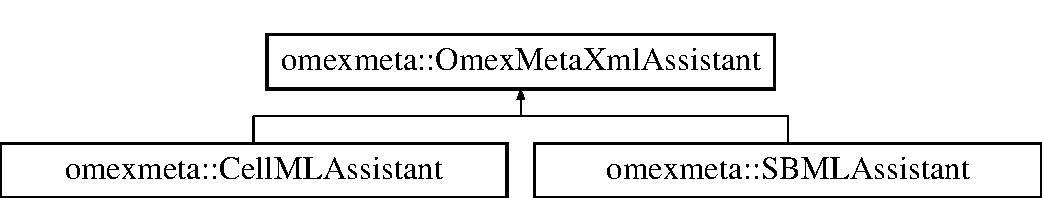
\includegraphics[height=2.000000cm]{classomexmeta_1_1OmexMetaXmlAssistant}
\end{center}
\end{figure}
\doxysubsection*{Public Member Functions}
\begin{DoxyCompactItemize}
\item 
const std\+::string \& \mbox{\hyperlink{classomexmeta_1_1OmexMetaXmlAssistant_a69bb3ac99f1585b6f567b80e88f52642}{get\+Metaid\+Base}} () const
\begin{DoxyCompactList}\small\item\em get the base for the metaid used by the current xml type. \mbox{\hyperlink{classThis}{This}} base is used as a precursor string for generating new metaids if requested by the user by setting generate\+\_\+new\+\_\+metaids=true. \end{DoxyCompactList}\item 
\mbox{\Hypertarget{classomexmeta_1_1OmexMetaXmlAssistant_a4c9759afd4af42595a4f0a4feb913524}\label{classomexmeta_1_1OmexMetaXmlAssistant_a4c9759afd4af42595a4f0a4feb913524}} 
int {\bfseries get\+Metaid\+Num\+Digits} () const
\item 
\mbox{\Hypertarget{classomexmeta_1_1OmexMetaXmlAssistant_a9ff89057f4fe7e8cb2e25f5431bf2bb5}\label{classomexmeta_1_1OmexMetaXmlAssistant_a9ff89057f4fe7e8cb2e25f5431bf2bb5}} 
bool {\bfseries generate\+New\+Metaids} () const
\item 
\mbox{\Hypertarget{classomexmeta_1_1OmexMetaXmlAssistant_af619a65dd28d04dfabd1930ff4110ce0}\label{classomexmeta_1_1OmexMetaXmlAssistant_af619a65dd28d04dfabd1930ff4110ce0}} 
{\bfseries Omex\+Meta\+Xml\+Assistant} (std\+::string xml, std\+::string metaid\+\_\+base=\char`\"{}Meta\+ID\char`\"{}, int metaid\+\_\+num\+\_\+digits=4, bool generate\+\_\+new\+\_\+metaids=false)
\item 
\mbox{\Hypertarget{classomexmeta_1_1OmexMetaXmlAssistant_aeef7e70a554aaf70fb694297e37e7cc8}\label{classomexmeta_1_1OmexMetaXmlAssistant_aeef7e70a554aaf70fb694297e37e7cc8}} 
std\+::pair$<$ std\+::string, std\+::vector$<$ std\+::string $>$ $>$ {\bfseries add\+Meta\+Ids} ()
\item 
\mbox{\Hypertarget{classomexmeta_1_1OmexMetaXmlAssistant_a3a6631e92df490f87f469abca81e1ba1}\label{classomexmeta_1_1OmexMetaXmlAssistant_a3a6631e92df490f87f469abca81e1ba1}} 
virtual std\+::vector$<$ std\+::string $>$ {\bfseries get\+Valid\+Elements} () const
\item 
\mbox{\Hypertarget{classomexmeta_1_1OmexMetaXmlAssistant_adbfc8d96f2adffa35ee01726a97dbcce}\label{classomexmeta_1_1OmexMetaXmlAssistant_adbfc8d96f2adffa35ee01726a97dbcce}} 
virtual std\+::string {\bfseries meta\+Id\+Tag\+Name} () const
\item 
\mbox{\Hypertarget{classomexmeta_1_1OmexMetaXmlAssistant_a9d178086ee6fe1d74e683476783ed933}\label{classomexmeta_1_1OmexMetaXmlAssistant_a9d178086ee6fe1d74e683476783ed933}} 
virtual std\+::string {\bfseries meta\+Id\+Namespace} () const
\end{DoxyCompactItemize}


\doxysubsection{Member Function Documentation}
\mbox{\Hypertarget{classomexmeta_1_1OmexMetaXmlAssistant_a69bb3ac99f1585b6f567b80e88f52642}\label{classomexmeta_1_1OmexMetaXmlAssistant_a69bb3ac99f1585b6f567b80e88f52642}} 
\index{omexmeta::OmexMetaXmlAssistant@{omexmeta::OmexMetaXmlAssistant}!getMetaidBase@{getMetaidBase}}
\index{getMetaidBase@{getMetaidBase}!omexmeta::OmexMetaXmlAssistant@{omexmeta::OmexMetaXmlAssistant}}
\doxysubsubsection{\texorpdfstring{getMetaidBase()}{getMetaidBase()}}
{\footnotesize\ttfamily const std\+::string \& omexmeta\+::\+Omex\+Meta\+Xml\+Assistant\+::get\+Metaid\+Base (\begin{DoxyParamCaption}{ }\end{DoxyParamCaption}) const}



get the base for the metaid used by the current xml type. \mbox{\hyperlink{classThis}{This}} base is used as a precursor string for generating new metaids if requested by the user by setting generate\+\_\+new\+\_\+metaids=true. 

the base is given as argument to the \mbox{\hyperlink{classomexmeta_1_1OmexMetaXmlAssistant}{Omex\+Meta\+Xml\+Assistant}} on instantiation. If base is \char`\"{}metaid\char`\"{} then ids generated will be metaid\+\_\+0000 

The documentation for this class was generated from the following files\+:\begin{DoxyCompactItemize}
\item 
src/omexmeta/include/omexmeta/Omex\+Meta\+Xml\+Assistant.\+h\item 
src/omexmeta/Omex\+Meta\+Xml\+Assistant.\+cpp\end{DoxyCompactItemize}

\hypertarget{structPair}{}\doxysection{Pair$<$ First, Second $>$ Struct Template Reference}
\label{structPair}\index{Pair$<$ First, Second $>$@{Pair$<$ First, Second $>$}}
\doxysubsection*{Public Attributes}
\begin{DoxyCompactItemize}
\item 
\mbox{\Hypertarget{structPair_acccddd6bdff96957a1e0714e539ef256}\label{structPair_acccddd6bdff96957a1e0714e539ef256}} 
First {\bfseries first}
\item 
\mbox{\Hypertarget{structPair_a86b9ae89026109ed31635f6c938b5b57}\label{structPair_a86b9ae89026109ed31635f6c938b5b57}} 
Second {\bfseries second}
\end{DoxyCompactItemize}


The documentation for this struct was generated from the following file\+:\begin{DoxyCompactItemize}
\item 
src/omexmeta/include/omexmeta/logger.\+h\end{DoxyCompactItemize}

\hypertarget{classomexmeta_1_1Participant}{}\doxysection{omexmeta\+::Participant Class Reference}
\label{classomexmeta_1_1Participant}\index{omexmeta::Participant@{omexmeta::Participant}}
Inheritance diagram for omexmeta\+::Participant\+:\begin{figure}[H]
\begin{center}
\leavevmode
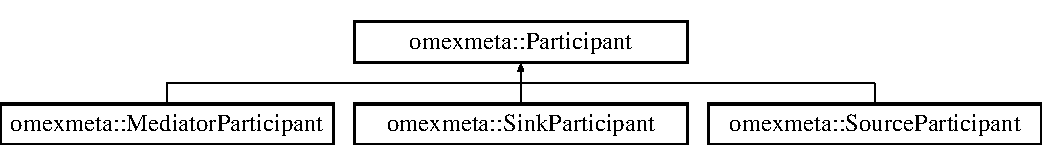
\includegraphics[height=1.954625cm]{classomexmeta_1_1Participant}
\end{center}
\end{figure}
\doxysubsection*{Public Member Functions}
\begin{DoxyCompactItemize}
\item 
void \mbox{\hyperlink{classomexmeta_1_1Participant_aee7846dcbb910dd394a0683841ab723a}{set\+Multiplier}} (double multiplier)
\begin{DoxyCompactList}\small\item\em return the vector of strings that keeps track of newly generated metaids. \mbox{\hyperlink{classThis}{This}} mechanism ensures unique metaids in the situation where the user has added $>$1 participant of a certain type i.\+e. sink. \end{DoxyCompactList}\item 
void \mbox{\hyperlink{classomexmeta_1_1Participant_a415c1205762dff6943426d830d74edcd}{set\+Physical\+Entity\+Reference}} (const std\+::string \&physical\+Entity\+Reference)
\begin{DoxyCompactList}\small\item\em setter for physical entity reference field of \mbox{\hyperlink{classomexmeta_1_1Participant}{Participant}} types \end{DoxyCompactList}\item 
const std\+::string \& \mbox{\hyperlink{classomexmeta_1_1Participant_a8a6626e17aca48b76465d66928eee78f}{get\+Local\+Participant\+Metaid}} () const
\begin{DoxyCompactList}\small\item\em return the local participant metaid. \end{DoxyCompactList}\item 
void \mbox{\hyperlink{classomexmeta_1_1Participant_a5e8f680950f55230587c0f85498c5047}{set\+Unique\+Participant\+Metaid}} (const std\+::string \&unique\+Participant\+Metaid)
\begin{DoxyCompactList}\small\item\em set the local participant metaid. \end{DoxyCompactList}\item 
\mbox{\Hypertarget{classomexmeta_1_1Participant_a6bf4c724ab5212d10f2a89893f369cd1}\label{classomexmeta_1_1Participant_a6bf4c724ab5212d10f2a89893f369cd1}} 
const std\+::string \& \mbox{\hyperlink{classomexmeta_1_1Participant_a6bf4c724ab5212d10f2a89893f369cd1}{get\+Local\+Uri}} () const
\begin{DoxyCompactList}\small\item\em getter for local uri attribute \end{DoxyCompactList}\item 
\mbox{\Hypertarget{classomexmeta_1_1Participant_a595323ae0681f42a7ba5981e2ee840f1}\label{classomexmeta_1_1Participant_a595323ae0681f42a7ba5981e2ee840f1}} 
void \mbox{\hyperlink{classomexmeta_1_1Participant_a595323ae0681f42a7ba5981e2ee840f1}{set\+Local\+Uri}} (const std\+::string \&local\+Uri)
\begin{DoxyCompactList}\small\item\em setter for local uri attribute \end{DoxyCompactList}\item 
void \mbox{\hyperlink{classomexmeta_1_1Participant_a395bc8d2561149a77371ed80e2ed1517}{free}} ()
\item 
\mbox{\hyperlink{classomexmeta_1_1Participant_ad7fb4564c20db459f8f9f8fc0b62ee09}{Participant}} (librdf\+\_\+model $\ast$model, std\+::string base\+\_\+metaid, const std\+::string \&model\+\_\+uri, const std\+::string \&local\+\_\+uri, std\+::string semsim\+\_\+predicate\+\_\+term, double multiplier, std\+::string physical\+Entity\+Reference, e\+Uri\+Type type)
\begin{DoxyCompactList}\small\item\em Superclass of participant types. \end{DoxyCompactList}\item 
\mbox{\Hypertarget{classomexmeta_1_1Participant_ad3db317039b403fdb7728885152cbeda}\label{classomexmeta_1_1Participant_ad3db317039b403fdb7728885152cbeda}} 
bool {\bfseries operator==} (const \mbox{\hyperlink{classomexmeta_1_1Participant}{Participant}} \&rhs) const
\item 
\mbox{\Hypertarget{classomexmeta_1_1Participant_aa4baa62cb4ccffe8443262382490328d}\label{classomexmeta_1_1Participant_aa4baa62cb4ccffe8443262382490328d}} 
bool {\bfseries operator!=} (const \mbox{\hyperlink{classomexmeta_1_1Participant}{Participant}} \&rhs) const
\item 
\mbox{\hyperlink{classomexmeta_1_1Triples}{Triples}} \mbox{\hyperlink{classomexmeta_1_1Participant_a278a5e9eaf13f5a7e195e38104eb7b12}{to\+Triples}} (std\+::string subject\+\_\+metaid, std\+::vector$<$ std\+::string $>$ \&metaid\+\_\+exclusions)
\begin{DoxyCompactList}\small\item\em create a \mbox{\hyperlink{classomexmeta_1_1Triples}{Triples}} object from the \mbox{\hyperlink{classomexmeta_1_1Participant}{Participant}}. \end{DoxyCompactList}\item 
std\+::string \mbox{\hyperlink{classomexmeta_1_1Participant_a03a1ffc7e9efaed5c0e94a62f7c72650}{create\+Metaid}} (const std\+::string \&base, std\+::vector$<$ std\+::string $>$ \&metaid\+\_\+exclusions) const
\begin{DoxyCompactList}\small\item\em create a new metaid use base \end{DoxyCompactList}\item 
std\+::basic\+\_\+string$<$ char $>$ \mbox{\hyperlink{classomexmeta_1_1Participant_aa09f8c5736dd172b03d7898519d9478d}{get\+Predicate}} ()
\begin{DoxyCompactList}\small\item\em get the predicate currently in use by the participant \end{DoxyCompactList}\item 
void \mbox{\hyperlink{classomexmeta_1_1Participant_a1188d6a2036514eb6b649ce1e08eca4d}{set\+Predicate}} (const std\+::string \&semsim\+\_\+predicate\+\_\+string)
\begin{DoxyCompactList}\small\item\em set the predicate used in the participant \end{DoxyCompactList}\item 
const std\+::string \& \mbox{\hyperlink{classomexmeta_1_1Participant_a232d2e7fe124ee13650d666fdfc3b866}{get\+Subject}} () const
\begin{DoxyCompactList}\small\item\em get the subject portion of the \mbox{\hyperlink{classomexmeta_1_1Participant}{Participant}}, which is the \end{DoxyCompactList}\item 
double \mbox{\hyperlink{classomexmeta_1_1Participant_a79b467cfc699483fdfe5e7686cc5447e}{get\+Multiplier}} () const
\begin{DoxyCompactList}\small\item\em get the multiplier representing the stoiciometry of the process being described \end{DoxyCompactList}\item 
const std\+::string \& \mbox{\hyperlink{classomexmeta_1_1Participant_a40a5858db6aaae7ec7095b320de838d1}{get\+Physical\+Entity\+Reference}} () const
\begin{DoxyCompactList}\small\item\em get the physical\+Entity\+Reference \end{DoxyCompactList}\item 
\mbox{\Hypertarget{classomexmeta_1_1Participant_ae78613f8d39ccfc23fc3624deb960fb0}\label{classomexmeta_1_1Participant_ae78613f8d39ccfc23fc3624deb960fb0}} 
const std\+::string \& \mbox{\hyperlink{classomexmeta_1_1Participant_ae78613f8d39ccfc23fc3624deb960fb0}{get\+Model\+Uri}} () const
\begin{DoxyCompactList}\small\item\em getter for model\+\_\+uri\+\_\+ attribute \end{DoxyCompactList}\item 
\mbox{\Hypertarget{classomexmeta_1_1Participant_abea74e8605f7314a51db8dc723961462}\label{classomexmeta_1_1Participant_abea74e8605f7314a51db8dc723961462}} 
void \mbox{\hyperlink{classomexmeta_1_1Participant_abea74e8605f7314a51db8dc723961462}{set\+Model\+Uri}} (const std\+::string \&model\+\_\+uri)
\begin{DoxyCompactList}\small\item\em setter for model\+\_\+uri\+\_\+ attribute \end{DoxyCompactList}\end{DoxyCompactItemize}


\doxysubsection{Constructor \& Destructor Documentation}
\mbox{\Hypertarget{classomexmeta_1_1Participant_ad7fb4564c20db459f8f9f8fc0b62ee09}\label{classomexmeta_1_1Participant_ad7fb4564c20db459f8f9f8fc0b62ee09}} 
\index{omexmeta::Participant@{omexmeta::Participant}!Participant@{Participant}}
\index{Participant@{Participant}!omexmeta::Participant@{omexmeta::Participant}}
\doxysubsubsection{\texorpdfstring{Participant()}{Participant()}}
{\footnotesize\ttfamily omexmeta\+::\+Participant\+::\+Participant (\begin{DoxyParamCaption}\item[{librdf\+\_\+model $\ast$}]{model,  }\item[{std\+::string}]{base\+\_\+metaid,  }\item[{const std\+::string \&}]{model\+\_\+uri,  }\item[{const std\+::string \&}]{local\+\_\+uri,  }\item[{std\+::string}]{semsim\+\_\+predicate\+\_\+term,  }\item[{double}]{multiplier,  }\item[{std\+::string}]{physical\+Entity\+Reference,  }\item[{e\+Uri\+Type}]{type }\end{DoxyParamCaption})}



Superclass of participant types. 


\begin{DoxyParams}{Parameters}
{\em model} & pointer to the librdf\+\_\+model$\ast$ in use. Passed down from \mbox{\hyperlink{classomexmeta_1_1RDF}{R\+DF}}. \\
\hline
{\em base\+\_\+metaid} & the content of the participant base\+\_\+metaid. A valid metaid. \\
\hline
{\em semsim\+\_\+predicate\+\_\+term} & a string from the \mbox{\hyperlink{classomexmeta_1_1SemSim}{Sem\+Sim}} vocabulary. \\
\hline
{\em multiplier} & Specifies the stoiciometry for the \mbox{\hyperlink{classomexmeta_1_1Participant}{Participant}} in the process \\
\hline
{\em physical\+Entity\+Reference} & the ID of the physical\+Entity assicated with the \mbox{\hyperlink{classomexmeta_1_1Participant}{Participant}}\\
\hline
\end{DoxyParams}
\mbox{\hyperlink{classThis}{This}} class should not be used directly -\/ the subclasses should be preferred.

For developers -\/ \mbox{\hyperlink{classThis}{This}} superclass is implemented in order to substantially reduce code duplication in the subclasses. 

\doxysubsection{Member Function Documentation}
\mbox{\Hypertarget{classomexmeta_1_1Participant_a03a1ffc7e9efaed5c0e94a62f7c72650}\label{classomexmeta_1_1Participant_a03a1ffc7e9efaed5c0e94a62f7c72650}} 
\index{omexmeta::Participant@{omexmeta::Participant}!createMetaid@{createMetaid}}
\index{createMetaid@{createMetaid}!omexmeta::Participant@{omexmeta::Participant}}
\doxysubsubsection{\texorpdfstring{createMetaid()}{createMetaid()}}
{\footnotesize\ttfamily std\+::string omexmeta\+::\+Participant\+::create\+Metaid (\begin{DoxyParamCaption}\item[{const std\+::string \&}]{base,  }\item[{std\+::vector$<$ std\+::string $>$ \&}]{metaid\+\_\+exclusions }\end{DoxyParamCaption}) const}



create a new metaid use base 


\begin{DoxyParams}{Parameters}
{\em base} & \\
\hline
\end{DoxyParams}
\mbox{\Hypertarget{classomexmeta_1_1Participant_a395bc8d2561149a77371ed80e2ed1517}\label{classomexmeta_1_1Participant_a395bc8d2561149a77371ed80e2ed1517}} 
\index{omexmeta::Participant@{omexmeta::Participant}!free@{free}}
\index{free@{free}!omexmeta::Participant@{omexmeta::Participant}}
\doxysubsubsection{\texorpdfstring{free()}{free()}}
{\footnotesize\ttfamily void omexmeta\+::\+Participant\+::free (\begin{DoxyParamCaption}{ }\end{DoxyParamCaption})}

@biref currently more of a placeholder so as to not break the tests. todo remove this method, \mbox{\hyperlink{classomexmeta_1_1Triple}{Triple}} objects deal with memory for Participants. \mbox{\Hypertarget{classomexmeta_1_1Participant_a8a6626e17aca48b76465d66928eee78f}\label{classomexmeta_1_1Participant_a8a6626e17aca48b76465d66928eee78f}} 
\index{omexmeta::Participant@{omexmeta::Participant}!getLocalParticipantMetaid@{getLocalParticipantMetaid}}
\index{getLocalParticipantMetaid@{getLocalParticipantMetaid}!omexmeta::Participant@{omexmeta::Participant}}
\doxysubsubsection{\texorpdfstring{getLocalParticipantMetaid()}{getLocalParticipantMetaid()}}
{\footnotesize\ttfamily const std\+::string \& omexmeta\+::\+Participant\+::get\+Local\+Participant\+Metaid (\begin{DoxyParamCaption}{ }\end{DoxyParamCaption}) const}



return the local participant metaid. 

When \mbox{\hyperlink{classomexmeta_1_1Participant}{Participant}} types are created they are done so with a metaid that is local to the annotation document not to the model. \mbox{\Hypertarget{classomexmeta_1_1Participant_a79b467cfc699483fdfe5e7686cc5447e}\label{classomexmeta_1_1Participant_a79b467cfc699483fdfe5e7686cc5447e}} 
\index{omexmeta::Participant@{omexmeta::Participant}!getMultiplier@{getMultiplier}}
\index{getMultiplier@{getMultiplier}!omexmeta::Participant@{omexmeta::Participant}}
\doxysubsubsection{\texorpdfstring{getMultiplier()}{getMultiplier()}}
{\footnotesize\ttfamily double omexmeta\+::\+Participant\+::get\+Multiplier (\begin{DoxyParamCaption}{ }\end{DoxyParamCaption}) const}



get the multiplier representing the stoiciometry of the process being described 

\begin{DoxyReturn}{Returns}
the multiplier 
\end{DoxyReturn}
\mbox{\Hypertarget{classomexmeta_1_1Participant_a40a5858db6aaae7ec7095b320de838d1}\label{classomexmeta_1_1Participant_a40a5858db6aaae7ec7095b320de838d1}} 
\index{omexmeta::Participant@{omexmeta::Participant}!getPhysicalEntityReference@{getPhysicalEntityReference}}
\index{getPhysicalEntityReference@{getPhysicalEntityReference}!omexmeta::Participant@{omexmeta::Participant}}
\doxysubsubsection{\texorpdfstring{getPhysicalEntityReference()}{getPhysicalEntityReference()}}
{\footnotesize\ttfamily const std\+::string \& omexmeta\+::\+Participant\+::get\+Physical\+Entity\+Reference (\begin{DoxyParamCaption}{ }\end{DoxyParamCaption}) const}



get the physical\+Entity\+Reference 

\begin{DoxyReturn}{Returns}
the physical\+Entity\+Reference string 
\end{DoxyReturn}
\mbox{\Hypertarget{classomexmeta_1_1Participant_aa09f8c5736dd172b03d7898519d9478d}\label{classomexmeta_1_1Participant_aa09f8c5736dd172b03d7898519d9478d}} 
\index{omexmeta::Participant@{omexmeta::Participant}!getPredicate@{getPredicate}}
\index{getPredicate@{getPredicate}!omexmeta::Participant@{omexmeta::Participant}}
\doxysubsubsection{\texorpdfstring{getPredicate()}{getPredicate()}}
{\footnotesize\ttfamily std\+::basic\+\_\+string$<$ char $>$ omexmeta\+::\+Participant\+::get\+Predicate (\begin{DoxyParamCaption}{ }\end{DoxyParamCaption})}



get the predicate currently in use by the participant 

\begin{DoxyReturn}{Returns}
a \mbox{\hyperlink{classomexmeta_1_1SemSim}{Sem\+Sim}} predicate 
\end{DoxyReturn}
\mbox{\Hypertarget{classomexmeta_1_1Participant_a232d2e7fe124ee13650d666fdfc3b866}\label{classomexmeta_1_1Participant_a232d2e7fe124ee13650d666fdfc3b866}} 
\index{omexmeta::Participant@{omexmeta::Participant}!getSubject@{getSubject}}
\index{getSubject@{getSubject}!omexmeta::Participant@{omexmeta::Participant}}
\doxysubsubsection{\texorpdfstring{getSubject()}{getSubject()}}
{\footnotesize\ttfamily const std\+::string \& omexmeta\+::\+Participant\+::get\+Subject (\begin{DoxyParamCaption}{ }\end{DoxyParamCaption}) const}



get the subject portion of the \mbox{\hyperlink{classomexmeta_1_1Participant}{Participant}}, which is the 

\begin{DoxyReturn}{Returns}
the string of the subject value metaid of the \mbox{\hyperlink{classomexmeta_1_1Participant}{Participant}} 
\end{DoxyReturn}
\mbox{\Hypertarget{classomexmeta_1_1Participant_aee7846dcbb910dd394a0683841ab723a}\label{classomexmeta_1_1Participant_aee7846dcbb910dd394a0683841ab723a}} 
\index{omexmeta::Participant@{omexmeta::Participant}!setMultiplier@{setMultiplier}}
\index{setMultiplier@{setMultiplier}!omexmeta::Participant@{omexmeta::Participant}}
\doxysubsubsection{\texorpdfstring{setMultiplier()}{setMultiplier()}}
{\footnotesize\ttfamily void omexmeta\+::\+Participant\+::set\+Multiplier (\begin{DoxyParamCaption}\item[{double}]{multiplier }\end{DoxyParamCaption})}



return the vector of strings that keeps track of newly generated metaids. \mbox{\hyperlink{classThis}{This}} mechanism ensures unique metaids in the situation where the user has added $>$1 participant of a certain type i.\+e. sink. 

setter for the multiplier field of \mbox{\hyperlink{classomexmeta_1_1Participant}{Participant}} types \mbox{\Hypertarget{classomexmeta_1_1Participant_a415c1205762dff6943426d830d74edcd}\label{classomexmeta_1_1Participant_a415c1205762dff6943426d830d74edcd}} 
\index{omexmeta::Participant@{omexmeta::Participant}!setPhysicalEntityReference@{setPhysicalEntityReference}}
\index{setPhysicalEntityReference@{setPhysicalEntityReference}!omexmeta::Participant@{omexmeta::Participant}}
\doxysubsubsection{\texorpdfstring{setPhysicalEntityReference()}{setPhysicalEntityReference()}}
{\footnotesize\ttfamily void omexmeta\+::\+Participant\+::set\+Physical\+Entity\+Reference (\begin{DoxyParamCaption}\item[{const std\+::string \&}]{physical\+Entity\+Reference }\end{DoxyParamCaption})}



setter for physical entity reference field of \mbox{\hyperlink{classomexmeta_1_1Participant}{Participant}} types 

A physical entity reference must exist and point to a physical entity in the xml. \mbox{\Hypertarget{classomexmeta_1_1Participant_a1188d6a2036514eb6b649ce1e08eca4d}\label{classomexmeta_1_1Participant_a1188d6a2036514eb6b649ce1e08eca4d}} 
\index{omexmeta::Participant@{omexmeta::Participant}!setPredicate@{setPredicate}}
\index{setPredicate@{setPredicate}!omexmeta::Participant@{omexmeta::Participant}}
\doxysubsubsection{\texorpdfstring{setPredicate()}{setPredicate()}}
{\footnotesize\ttfamily void omexmeta\+::\+Participant\+::set\+Predicate (\begin{DoxyParamCaption}\item[{const std\+::string \&}]{semsim\+\_\+predicate\+\_\+string }\end{DoxyParamCaption})}



set the predicate used in the participant 


\begin{DoxyParams}{Parameters}
{\em semsim\+\_\+predicate\+\_\+string} & The predicate portion of the \mbox{\hyperlink{classomexmeta_1_1SemSim}{Sem\+Sim}} predicate you want to use.\\
\hline
\end{DoxyParams}
i.\+e. \char`\"{}has\+Source\+Participant\char`\"{} not \char`\"{}http\+://www.\+bhi.\+washington.\+edu/semsim\#has\+Source\+Participant\char`\"{} \mbox{\Hypertarget{classomexmeta_1_1Participant_a5e8f680950f55230587c0f85498c5047}\label{classomexmeta_1_1Participant_a5e8f680950f55230587c0f85498c5047}} 
\index{omexmeta::Participant@{omexmeta::Participant}!setUniqueParticipantMetaid@{setUniqueParticipantMetaid}}
\index{setUniqueParticipantMetaid@{setUniqueParticipantMetaid}!omexmeta::Participant@{omexmeta::Participant}}
\doxysubsubsection{\texorpdfstring{setUniqueParticipantMetaid()}{setUniqueParticipantMetaid()}}
{\footnotesize\ttfamily void omexmeta\+::\+Participant\+::set\+Unique\+Participant\+Metaid (\begin{DoxyParamCaption}\item[{const std\+::string \&}]{unique\+Participant\+Metaid }\end{DoxyParamCaption})}



set the local participant metaid. 

When \mbox{\hyperlink{classomexmeta_1_1Participant}{Participant}} types are created they are done so with a metaid that is local to the annotation document not to the model. \mbox{\Hypertarget{classomexmeta_1_1Participant_a278a5e9eaf13f5a7e195e38104eb7b12}\label{classomexmeta_1_1Participant_a278a5e9eaf13f5a7e195e38104eb7b12}} 
\index{omexmeta::Participant@{omexmeta::Participant}!toTriples@{toTriples}}
\index{toTriples@{toTriples}!omexmeta::Participant@{omexmeta::Participant}}
\doxysubsubsection{\texorpdfstring{toTriples()}{toTriples()}}
{\footnotesize\ttfamily \mbox{\hyperlink{classomexmeta_1_1Triples}{Triples}} omexmeta\+::\+Participant\+::to\+Triples (\begin{DoxyParamCaption}\item[{std\+::string}]{subject\+\_\+metaid,  }\item[{std\+::vector$<$ std\+::string $>$ \&}]{metaid\+\_\+exclusions }\end{DoxyParamCaption})}



create a \mbox{\hyperlink{classomexmeta_1_1Triples}{Triples}} object from the \mbox{\hyperlink{classomexmeta_1_1Participant}{Participant}}. 


\begin{DoxyParams}{Parameters}
{\em subject\+\_\+metaid} & the metaid for a process \\
\hline
\end{DoxyParams}
\begin{DoxyReturn}{Returns}
A \mbox{\hyperlink{classomexmeta_1_1Triples}{Triples}} container for the \mbox{\hyperlink{classomexmeta_1_1Triples}{Triples}} associated with this \mbox{\hyperlink{classomexmeta_1_1Participant}{Participant}}
\end{DoxyReturn}
The same to\+Triples method is used for all participants. Since \mbox{\hyperlink{classomexmeta_1_1Triple}{Triple}}\textquotesingle{}s are added to the model as a unit, we need a way of keeping track of which metaids have been used in order to ensure unique metaid\textquotesingle{}s when we have more than one Sink/\+Source/\+Mediate \mbox{\hyperlink{classomexmeta_1_1Participant}{Participant}}. For this we add the generated metaid to a vector. Note, we do this before concat with local uri because of the way local\+\_\+uri\textquotesingle{}s were added after the original design was in place. Future developers might want to look at this.

The documentation for this class was generated from the following files\+:\begin{DoxyCompactItemize}
\item 
src/omexmeta/include/omexmeta/Participant.\+h\item 
src/omexmeta/Participant.\+cpp\end{DoxyCompactItemize}

\hypertarget{classomexmeta_1_1PersonalInformation}{}\doxysection{omexmeta\+::Personal\+Information Class Reference}
\label{classomexmeta_1_1PersonalInformation}\index{omexmeta::PersonalInformation@{omexmeta::PersonalInformation}}


add personal information to the model as a composite annotation.  




{\ttfamily \#include $<$Personal\+Information.\+h$>$}

\doxysubsection*{Public Member Functions}
\begin{DoxyCompactItemize}
\item 
\mbox{\Hypertarget{classomexmeta_1_1PersonalInformation_a8ca987ddfc8c218bbcbdb548b186b2a2}\label{classomexmeta_1_1PersonalInformation_a8ca987ddfc8c218bbcbdb548b186b2a2}} 
const std\+::vector$<$ std\+::string $>$ \& {\bfseries get\+Namespaces} () const
\item 
\mbox{\Hypertarget{classomexmeta_1_1PersonalInformation_aaafb0d585de0eea7cb979e8fd7285228}\label{classomexmeta_1_1PersonalInformation_aaafb0d585de0eea7cb979e8fd7285228}} 
{\bfseries Personal\+Information} (librdf\+\_\+model $\ast$model, \mbox{\hyperlink{classomexmeta_1_1UriHandler}{Uri\+Handler}} \&uri\+Handler)
\item 
\mbox{\Hypertarget{classomexmeta_1_1PersonalInformation_a75cedb2a97efb996852b4e7cd39d6440}\label{classomexmeta_1_1PersonalInformation_a75cedb2a97efb996852b4e7cd39d6440}} 
\mbox{\hyperlink{classomexmeta_1_1PersonalInformation_a75cedb2a97efb996852b4e7cd39d6440}{Personal\+Information}} (const \mbox{\hyperlink{classomexmeta_1_1PersonalInformation}{Personal\+Information}} \&information)=delete
\begin{DoxyCompactList}\small\item\em Copy constructor for \mbox{\hyperlink{classomexmeta_1_1PersonalInformation}{Personal\+Information}}. \end{DoxyCompactList}\item 
\mbox{\hyperlink{classomexmeta_1_1PersonalInformation_a6653d6c5751154f5f33562d9879d6727}{Personal\+Information}} (\mbox{\hyperlink{classomexmeta_1_1PersonalInformation}{Personal\+Information}} \&\&information) noexcept
\begin{DoxyCompactList}\small\item\em Move constructor for \mbox{\hyperlink{classomexmeta_1_1PersonalInformation}{Personal\+Information}}. \end{DoxyCompactList}\item 
\mbox{\Hypertarget{classomexmeta_1_1PersonalInformation_a11a759dd5f065ba6a48f0bc3b4c48438}\label{classomexmeta_1_1PersonalInformation_a11a759dd5f065ba6a48f0bc3b4c48438}} 
\mbox{\hyperlink{classomexmeta_1_1PersonalInformation}{Personal\+Information}} \& \mbox{\hyperlink{classomexmeta_1_1PersonalInformation_a11a759dd5f065ba6a48f0bc3b4c48438}{operator=}} (const \mbox{\hyperlink{classomexmeta_1_1PersonalInformation}{Personal\+Information}} \&information)=delete
\begin{DoxyCompactList}\small\item\em assignment operator for \mbox{\hyperlink{classomexmeta_1_1PersonalInformation}{Personal\+Information}} \end{DoxyCompactList}\item 
\mbox{\hyperlink{classomexmeta_1_1PersonalInformation}{Personal\+Information}} \& \mbox{\hyperlink{classomexmeta_1_1PersonalInformation_a048a3377b27d4b87681e4f8c24dd8c4f}{operator=}} (\mbox{\hyperlink{classomexmeta_1_1PersonalInformation}{Personal\+Information}} \&\&information) noexcept
\begin{DoxyCompactList}\small\item\em move assignment operator for \mbox{\hyperlink{classomexmeta_1_1PersonalInformation}{Personal\+Information}} \end{DoxyCompactList}\item 
\mbox{\Hypertarget{classomexmeta_1_1PersonalInformation_aef8b8cfd83f8247b487d58f887c93e54}\label{classomexmeta_1_1PersonalInformation_aef8b8cfd83f8247b487d58f887c93e54}} 
const std\+::string \& {\bfseries get\+Local\+Uri} () const
\item 
\mbox{\Hypertarget{classomexmeta_1_1PersonalInformation_a84ce9ae11ad2ed4a01fe1b5b84707146}\label{classomexmeta_1_1PersonalInformation_a84ce9ae11ad2ed4a01fe1b5b84707146}} 
bool {\bfseries operator==} (const \mbox{\hyperlink{classomexmeta_1_1PersonalInformation}{Personal\+Information}} \&rhs) const
\item 
\mbox{\Hypertarget{classomexmeta_1_1PersonalInformation_abb71bc363efd7466c71733709aa50394}\label{classomexmeta_1_1PersonalInformation_abb71bc363efd7466c71733709aa50394}} 
bool {\bfseries operator!=} (const \mbox{\hyperlink{classomexmeta_1_1PersonalInformation}{Personal\+Information}} \&rhs) const
\item 
\mbox{\Hypertarget{classomexmeta_1_1PersonalInformation_af37c1c7065dd9edbb89e90e8b37f35e8}\label{classomexmeta_1_1PersonalInformation_af37c1c7065dd9edbb89e90e8b37f35e8}} 
\mbox{\hyperlink{classomexmeta_1_1PersonalInformation}{Personal\+Information}} \& {\bfseries add\+Creator} (const std\+::string \&value)
\item 
\mbox{\Hypertarget{classomexmeta_1_1PersonalInformation_a14d941856c6a188a964fb4a0c5475885}\label{classomexmeta_1_1PersonalInformation_a14d941856c6a188a964fb4a0c5475885}} 
\mbox{\hyperlink{classomexmeta_1_1PersonalInformation}{Personal\+Information}} \& {\bfseries add\+Name} (const std\+::string \&value)
\item 
\mbox{\Hypertarget{classomexmeta_1_1PersonalInformation_aab4c7522fba200d4776d59c32085371d}\label{classomexmeta_1_1PersonalInformation_aab4c7522fba200d4776d59c32085371d}} 
\mbox{\hyperlink{classomexmeta_1_1PersonalInformation}{Personal\+Information}} \& {\bfseries add\+Mbox} (const std\+::string \&value)
\item 
\mbox{\Hypertarget{classomexmeta_1_1PersonalInformation_a9fd33e3189e1f77725e54dd24cc9dcb7}\label{classomexmeta_1_1PersonalInformation_a9fd33e3189e1f77725e54dd24cc9dcb7}} 
\mbox{\hyperlink{classomexmeta_1_1PersonalInformation}{Personal\+Information}} \& {\bfseries add\+Account\+Name} (const std\+::string \&value)
\item 
\mbox{\Hypertarget{classomexmeta_1_1PersonalInformation_a344fc47bde65f8c0ea75409160fdfe00}\label{classomexmeta_1_1PersonalInformation_a344fc47bde65f8c0ea75409160fdfe00}} 
\mbox{\hyperlink{classomexmeta_1_1PersonalInformation}{Personal\+Information}} \& {\bfseries add\+Account\+Service\+Homepage} (const std\+::string \&value)
\item 
\mbox{\Hypertarget{classomexmeta_1_1PersonalInformation_af26bf72dc840b9c45fa7494f7164c04d}\label{classomexmeta_1_1PersonalInformation_af26bf72dc840b9c45fa7494f7164c04d}} 
\mbox{\hyperlink{classomexmeta_1_1PersonalInformation}{Personal\+Information}} \& {\bfseries add\+Foaf\+Blank} (const std\+::string \&predicate, const std\+::string \&blank\+\_\+value)
\item 
\mbox{\Hypertarget{classomexmeta_1_1PersonalInformation_a1df32d40f46d98767fc360015bf0f3ed}\label{classomexmeta_1_1PersonalInformation_a1df32d40f46d98767fc360015bf0f3ed}} 
\mbox{\hyperlink{classomexmeta_1_1PersonalInformation}{Personal\+Information}} \& {\bfseries add\+DC} (const std\+::string \&predicate, const \mbox{\hyperlink{classredland_1_1LibrdfNode}{Librdf\+Node}} \&value\+\_\+node)
\item 
\mbox{\Hypertarget{classomexmeta_1_1PersonalInformation_a1458c6e092a9436a956ffd6a92c71d16}\label{classomexmeta_1_1PersonalInformation_a1458c6e092a9436a956ffd6a92c71d16}} 
\mbox{\hyperlink{classomexmeta_1_1PersonalInformation}{Personal\+Information}} \& {\bfseries add\+DCBlank} (const std\+::string \&predicate, const std\+::string \&blank\+\_\+value)
\item 
\mbox{\Hypertarget{classomexmeta_1_1PersonalInformation_a1c605320ec0f12dda246cc3abdb0aeae}\label{classomexmeta_1_1PersonalInformation_a1c605320ec0f12dda246cc3abdb0aeae}} 
\mbox{\hyperlink{classomexmeta_1_1PersonalInformation}{Personal\+Information}} \& {\bfseries add\+DCUri} (const std\+::string \&predicate, const std\+::string \&uri\+\_\+value)
\item 
\mbox{\Hypertarget{classomexmeta_1_1PersonalInformation_a843d2eddcdb33fc49d7de5059f5fa04c}\label{classomexmeta_1_1PersonalInformation_a843d2eddcdb33fc49d7de5059f5fa04c}} 
\mbox{\hyperlink{classomexmeta_1_1PersonalInformation}{Personal\+Information}} \& {\bfseries add\+DCLiteral} (const std\+::string \&predicate, const std\+::string \&literal\+\_\+value)
\item 
\mbox{\Hypertarget{classomexmeta_1_1PersonalInformation_a7d760a327fe103386f1bb08063f8795a}\label{classomexmeta_1_1PersonalInformation_a7d760a327fe103386f1bb08063f8795a}} 
\mbox{\hyperlink{classomexmeta_1_1PersonalInformation}{Personal\+Information}} \& {\bfseries add\+Foaf\+Uri} (const std\+::string \&predicate, const std\+::string \&uri\+\_\+value)
\item 
\mbox{\Hypertarget{classomexmeta_1_1PersonalInformation_ae6fbd4fad2a738fae9fce7affa6b2f15}\label{classomexmeta_1_1PersonalInformation_ae6fbd4fad2a738fae9fce7affa6b2f15}} 
\mbox{\hyperlink{classomexmeta_1_1PersonalInformation}{Personal\+Information}} \& {\bfseries add\+Foaf\+Literal} (const std\+::string \&predicate, const std\+::string \&literal\+\_\+value)
\item 
\mbox{\Hypertarget{classomexmeta_1_1PersonalInformation_a99198226df0c8acfdd7bc30ff7c4bf8b}\label{classomexmeta_1_1PersonalInformation_a99198226df0c8acfdd7bc30ff7c4bf8b}} 
\mbox{\hyperlink{classomexmeta_1_1PersonalInformation}{Personal\+Information}} \& {\bfseries add\+Foaf} (const std\+::string \&predicate, const \mbox{\hyperlink{classredland_1_1LibrdfNode}{Librdf\+Node}} \&value\+\_\+node)
\item 
\mbox{\Hypertarget{classomexmeta_1_1PersonalInformation_ae00bfe55d51745ac11f37986443feb28}\label{classomexmeta_1_1PersonalInformation_ae00bfe55d51745ac11f37986443feb28}} 
const std\+::string \& {\bfseries get\+Metaid} () const
\item 
\mbox{\Hypertarget{classomexmeta_1_1PersonalInformation_a2bf7f31511c545eb0158643645115b00}\label{classomexmeta_1_1PersonalInformation_a2bf7f31511c545eb0158643645115b00}} 
void {\bfseries set\+Metaid} (const std\+::string \&metaid)
\item 
\mbox{\Hypertarget{classomexmeta_1_1PersonalInformation_a6b2ce3a6c724b67afe3d0c2df00bb484}\label{classomexmeta_1_1PersonalInformation_a6b2ce3a6c724b67afe3d0c2df00bb484}} 
const std\+::string \& {\bfseries get\+Model\+Uri} () const
\item 
\mbox{\Hypertarget{classomexmeta_1_1PersonalInformation_aecc5783753b41ed88a49c5b3bce82ba4}\label{classomexmeta_1_1PersonalInformation_aecc5783753b41ed88a49c5b3bce82ba4}} 
\mbox{\hyperlink{classomexmeta_1_1Triples}{Triples}} {\bfseries get\+Triples} ()
\item 
\mbox{\Hypertarget{classomexmeta_1_1PersonalInformation_aea3a34c765f176a3d6f6b88a6b8c8369}\label{classomexmeta_1_1PersonalInformation_aea3a34c765f176a3d6f6b88a6b8c8369}} 
void {\bfseries free\+Triples} ()
\item 
\mbox{\Hypertarget{classomexmeta_1_1PersonalInformation_a25a1e9ba56dda2459cb1bbbe61cc4346}\label{classomexmeta_1_1PersonalInformation_a25a1e9ba56dda2459cb1bbbe61cc4346}} 
void {\bfseries set\+Triples} (\mbox{\hyperlink{classomexmeta_1_1Triples}{Triples}} triples)
\end{DoxyCompactItemize}


\doxysubsection{Detailed Description}
add personal information to the model as a composite annotation. 

For developers\+: \mbox{\hyperlink{classThis}{This}} composite annotation is fundamentally different to the Physical$\ast$ composites in that the structure is more arbitrary. With the Physical$\ast$ composites, the structure is very well defined, so it was easier to implement the to\+Triples() method to construct those triples when called. \mbox{\hyperlink{classThis}{This}} differs subtly in \mbox{\hyperlink{classomexmeta_1_1PersonalInformation}{Personal\+Information}} in that we have a class level \mbox{\hyperlink{classomexmeta_1_1Triples}{Triples}} object to store generated triples using a series of methods. The user can use as many or few of them as they like. Once finished they can use the get\+Triples() method to get a unique ptr to the triples. 

\doxysubsection{Constructor \& Destructor Documentation}
\mbox{\Hypertarget{classomexmeta_1_1PersonalInformation_a6653d6c5751154f5f33562d9879d6727}\label{classomexmeta_1_1PersonalInformation_a6653d6c5751154f5f33562d9879d6727}} 
\index{omexmeta::PersonalInformation@{omexmeta::PersonalInformation}!PersonalInformation@{PersonalInformation}}
\index{PersonalInformation@{PersonalInformation}!omexmeta::PersonalInformation@{omexmeta::PersonalInformation}}
\doxysubsubsection{\texorpdfstring{PersonalInformation()}{PersonalInformation()}}
{\footnotesize\ttfamily omexmeta\+::\+Personal\+Information\+::\+Personal\+Information (\begin{DoxyParamCaption}\item[{\mbox{\hyperlink{classomexmeta_1_1PersonalInformation}{Personal\+Information}} \&\&}]{information }\end{DoxyParamCaption})\hspace{0.3cm}{\ttfamily [noexcept]}}



Move constructor for \mbox{\hyperlink{classomexmeta_1_1PersonalInformation}{Personal\+Information}}. 

move constructor 

\doxysubsection{Member Function Documentation}
\mbox{\Hypertarget{classomexmeta_1_1PersonalInformation_a048a3377b27d4b87681e4f8c24dd8c4f}\label{classomexmeta_1_1PersonalInformation_a048a3377b27d4b87681e4f8c24dd8c4f}} 
\index{omexmeta::PersonalInformation@{omexmeta::PersonalInformation}!operator=@{operator=}}
\index{operator=@{operator=}!omexmeta::PersonalInformation@{omexmeta::PersonalInformation}}
\doxysubsubsection{\texorpdfstring{operator=()}{operator=()}}
{\footnotesize\ttfamily \mbox{\hyperlink{classomexmeta_1_1PersonalInformation}{Personal\+Information}} \& omexmeta\+::\+Personal\+Information\+::operator= (\begin{DoxyParamCaption}\item[{\mbox{\hyperlink{classomexmeta_1_1PersonalInformation}{Personal\+Information}} \&\&}]{information }\end{DoxyParamCaption})\hspace{0.3cm}{\ttfamily [noexcept]}}



move assignment operator for \mbox{\hyperlink{classomexmeta_1_1PersonalInformation}{Personal\+Information}} 

move assignment constructor 

The documentation for this class was generated from the following files\+:\begin{DoxyCompactItemize}
\item 
src/omexmeta/include/omexmeta/Personal\+Information.\+h\item 
src/omexmeta/Personal\+Information.\+cpp\end{DoxyCompactItemize}

\hypertarget{classomexmeta_1_1PhysicalEntity}{}\section{omexmeta\+:\+:Physical\+Entity Class Reference}
\label{classomexmeta_1_1PhysicalEntity}\index{omexmeta\+::\+Physical\+Entity@{omexmeta\+::\+Physical\+Entity}}


{\ttfamily \#include $<$Physical\+Entity.\+h$>$}

Inheritance diagram for omexmeta\+:\+:Physical\+Entity\+:\begin{figure}[H]
\begin{center}
\leavevmode
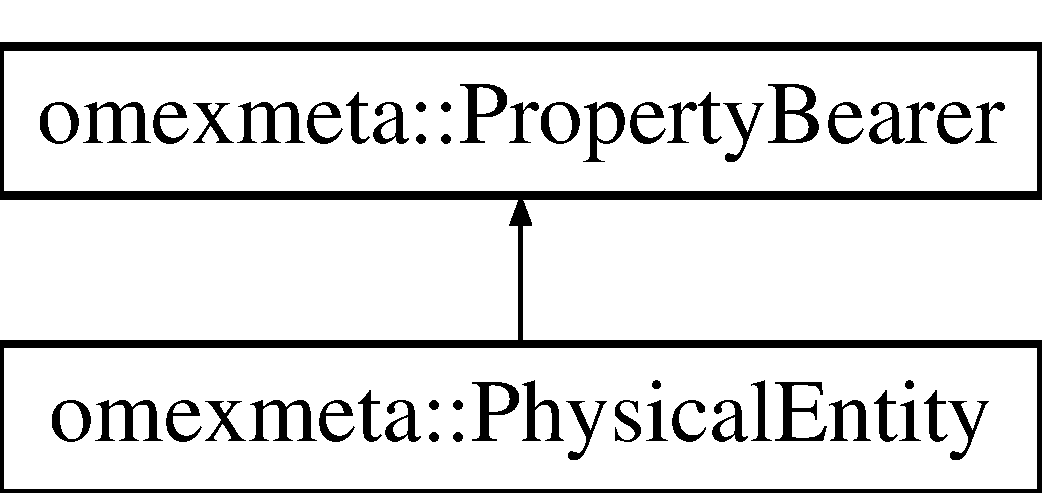
\includegraphics[height=2.000000cm]{classomexmeta_1_1PhysicalEntity}
\end{center}
\end{figure}
\subsection*{Public Member Functions}
\begin{DoxyCompactItemize}
\item 
\hyperlink{classomexmeta_1_1PhysicalEntity_a9d29348a080c64f91ff6ec184fd45ece}{Physical\+Entity} ()=delete
\begin{DoxyCompactList}\small\item\em default constructor for \hyperlink{classomexmeta_1_1PhysicalEntity}{Physical\+Entity} \end{DoxyCompactList}\item 
\hyperlink{classomexmeta_1_1PhysicalEntity_a0341918665af91cacdb4481d037c42d2}{Physical\+Entity} (librdf\+\_\+model $\ast$model, std\+::string model\+\_\+uri, std\+::string local\+\_\+uri, \hyperlink{classomexmeta_1_1PhysicalProperty}{Physical\+Property} physical\+Property, \hyperlink{classomexmeta_1_1Resource}{Resource} \hyperlink{classomexmeta_1_1PhysicalEntity_a2498e9b0b11a00200e47332c4515b1f1}{is}, Resources is\+\_\+part\+\_\+of)
\begin{DoxyCompactList}\small\item\em constructor for instantiating a \hyperlink{classomexmeta_1_1PhysicalEntity}{Physical\+Entity} object \end{DoxyCompactList}\item 
void \hyperlink{classomexmeta_1_1PhysicalEntity_a6fd4acd7255a01322c4a53d3e84df0ba}{free} ()
\begin{DoxyCompactList}\small\item\em free resources uses by \hyperlink{classomexmeta_1_1PhysicalEntity}{Physical\+Entity} \end{DoxyCompactList}\item 
\hyperlink{classomexmeta_1_1PhysicalEntity_a6bbbce71778e374de7d4e5e2e674fc2b}{Physical\+Entity} (librdf\+\_\+model $\ast$model)
\begin{DoxyCompactList}\small\item\em constructor for \hyperlink{classomexmeta_1_1PhysicalEntity}{Physical\+Entity} object. \end{DoxyCompactList}\item 
\hyperlink{classomexmeta_1_1PhysicalEntity_a5f583e60ad44bbb3dfcd11fdc6bc72cc}{Physical\+Entity} (librdf\+\_\+model $\ast$model, const std\+::string \&model\+\_\+uri, const std\+::string \&local\+\_\+uri)
\begin{DoxyCompactList}\small\item\em constructor for \hyperlink{classomexmeta_1_1PhysicalEntity}{Physical\+Entity} object. \end{DoxyCompactList}\item 
\hyperlink{classomexmeta_1_1Triples}{Triples} \hyperlink{classomexmeta_1_1PhysicalEntity_a51f5df8b2e8a1d65e5aa0d10e53b77ba}{to\+Triples} () override
\begin{DoxyCompactList}\small\item\em convert \hyperlink{classomexmeta_1_1PhysicalEntity}{Physical\+Entity} to a \hyperlink{classomexmeta_1_1Triples}{Triples} object, which can then be passed to a model via the \hyperlink{classomexmeta_1_1Editor_a0740831baafe244374ad7a324d51a87e}{Editor\+::add\+Physical\+Entity} method. \end{DoxyCompactList}\item 
const \hyperlink{classomexmeta_1_1Resource}{Resource} \& \hyperlink{classomexmeta_1_1PhysicalEntity_ae4b3374e9ebb817eb63f9105b491e958}{get\+Identity\+Resource} () const
\begin{DoxyCompactList}\small\item\em return the Identity\+Resource in use. I.\+e. the \char`\"{}what\char`\"{} portion of the \hyperlink{classomexmeta_1_1PhysicalEntity}{Physical\+Entity} \end{DoxyCompactList}\item 
const Resources \& \hyperlink{classomexmeta_1_1PhysicalEntity_a3e2fba07a4622db0180650d24bf263d9}{get\+Location\+Resources} () const
\begin{DoxyCompactList}\small\item\em return a vector of resources representing the \char`\"{}where\char`\"{} part of the \hyperlink{classomexmeta_1_1PhysicalEntity}{Physical\+Entity} \end{DoxyCompactList}\item 
\hyperlink{classomexmeta_1_1PhysicalEntity}{Physical\+Entity} \& \hyperlink{classomexmeta_1_1PhysicalEntity_a5d7168c527d2dbdacd612de37aa9a605}{set\+Physical\+Property} (std\+::string subject\+\_\+metaid, const std\+::string \&physical\+Property)
\begin{DoxyCompactList}\small\item\em sets the physical property for a \hyperlink{classomexmeta_1_1PhysicalEntity}{Physical\+Entity} instance. \end{DoxyCompactList}\item 
\hyperlink{classomexmeta_1_1PhysicalEntity}{Physical\+Entity} \& \hyperlink{classomexmeta_1_1PhysicalEntity_a9bca0cb13601b6f9617df9f264968f1f}{set\+Physical\+Property} (\hyperlink{classomexmeta_1_1PhysicalProperty}{Physical\+Property} physical\+Property)
\begin{DoxyCompactList}\small\item\em sets the physical property for a \hyperlink{classomexmeta_1_1PhysicalEntity}{Physical\+Entity} instance \end{DoxyCompactList}\item 
\hyperlink{classomexmeta_1_1PhysicalEntity}{Physical\+Entity} \& \hyperlink{classomexmeta_1_1PhysicalEntity_a4d4c3ee9572b19e44e79a44f18f1ac31}{set\+Identity} (const std\+::string \&resource)
\begin{DoxyCompactList}\small\item\em sets the identity portion of the \hyperlink{classomexmeta_1_1PhysicalEntity}{Physical\+Entity} (the \char`\"{}\+What\char`\"{}). \end{DoxyCompactList}\item 
\hyperlink{classomexmeta_1_1PhysicalEntity}{Physical\+Entity} \& \hyperlink{classomexmeta_1_1PhysicalEntity_a82e77be3327c537b2426b571afaa5045}{add\+Location} (const std\+::string \&where)
\begin{DoxyCompactList}\small\item\em add a location to the \hyperlink{classomexmeta_1_1PhysicalEntity}{Physical\+Entity}. \end{DoxyCompactList}\item 
int \hyperlink{classomexmeta_1_1PhysicalEntity_a33559c90dbe3e3be1b71898ab9a5bfa4}{get\+Num\+Locations} () const
\begin{DoxyCompactList}\small\item\em returns the number of locations used by \hyperlink{classomexmeta_1_1PhysicalEntity}{Physical\+Entity} \end{DoxyCompactList}\item 
\mbox{\Hypertarget{classomexmeta_1_1PhysicalEntity_a5f54e5c2df0fd5c3b9121e1426b23af6}\label{classomexmeta_1_1PhysicalEntity_a5f54e5c2df0fd5c3b9121e1426b23af6}} 
bool {\bfseries operator==} (const \hyperlink{classomexmeta_1_1PhysicalEntity}{Physical\+Entity} \&rhs) const
\item 
\mbox{\Hypertarget{classomexmeta_1_1PhysicalEntity_afee546a420f16e128ed1add9fec35b4f}\label{classomexmeta_1_1PhysicalEntity_afee546a420f16e128ed1add9fec35b4f}} 
bool {\bfseries operator!=} (const \hyperlink{classomexmeta_1_1PhysicalEntity}{Physical\+Entity} \&rhs) const
\item 
\hyperlink{classomexmeta_1_1PhysicalEntity}{Physical\+Entity} \& \hyperlink{classomexmeta_1_1PhysicalEntity_a5399ef8eef084f2dd8b13ef537823d94}{is\+Version\+Of} (const std\+::string \&is\+\_\+version\+\_\+of)
\begin{DoxyCompactList}\small\item\em Set the is\+Version\+Of portion of the \hyperlink{classomexmeta_1_1PhysicalEntity}{Physical\+Entity} composite annotation. \end{DoxyCompactList}\item 
\hyperlink{classomexmeta_1_1PhysicalEntity}{Physical\+Entity} \& \hyperlink{classomexmeta_1_1PhysicalEntity_a1736d331705bf2f1569f492fc733949e}{set\+About} (const std\+::string \&about) override
\begin{DoxyCompactList}\small\item\em Set the about portion of the \hyperlink{classomexmeta_1_1PhysicalEntity}{Physical\+Entity} composite annotation. \end{DoxyCompactList}\item 
\hyperlink{classomexmeta_1_1PhysicalEntity}{Physical\+Entity} \& \hyperlink{classomexmeta_1_1PhysicalEntity_a2498e9b0b11a00200e47332c4515b1f1}{is} (const std\+::string \&is)
\begin{DoxyCompactList}\small\item\em Set the {\ttfamily is} portion of the \hyperlink{classomexmeta_1_1PhysicalEntity}{Physical\+Entity} composite annotation. \end{DoxyCompactList}\item 
\hyperlink{classomexmeta_1_1PhysicalEntity}{Physical\+Entity} \& \hyperlink{classomexmeta_1_1PhysicalEntity_a6a68c098a063d5a8416b83ae219eddca}{is\+Part\+Of} (const std\+::string \&\hyperlink{classomexmeta_1_1PhysicalEntity_a2498e9b0b11a00200e47332c4515b1f1}{is})
\begin{DoxyCompactList}\small\item\em Set the location ({\ttfamily is\+Part\+Of}) portion of the \hyperlink{classomexmeta_1_1PhysicalEntity}{Physical\+Entity} composite annotation. \end{DoxyCompactList}\end{DoxyCompactItemize}
\subsection*{Additional Inherited Members}


\subsection{Detailed Description}
The \hyperlink{classomexmeta_1_1PhysicalEntity}{Physical\+Entity} type of \hyperlink{classomexmeta_1_1PhysicalPhenomenon}{Physical\+Phenomenon} 

\subsection{Constructor \& Destructor Documentation}
\mbox{\Hypertarget{classomexmeta_1_1PhysicalEntity_a9d29348a080c64f91ff6ec184fd45ece}\label{classomexmeta_1_1PhysicalEntity_a9d29348a080c64f91ff6ec184fd45ece}} 
\index{omexmeta\+::\+Physical\+Entity@{omexmeta\+::\+Physical\+Entity}!Physical\+Entity@{Physical\+Entity}}
\index{Physical\+Entity@{Physical\+Entity}!omexmeta\+::\+Physical\+Entity@{omexmeta\+::\+Physical\+Entity}}
\subsubsection{\texorpdfstring{Physical\+Entity()}{PhysicalEntity()}\hspace{0.1cm}{\footnotesize\ttfamily [1/4]}}
{\footnotesize\ttfamily omexmeta\+::\+Physical\+Entity\+::\+Physical\+Entity (\begin{DoxyParamCaption}{ }\end{DoxyParamCaption})\hspace{0.3cm}{\ttfamily [delete]}}



default constructor for \hyperlink{classomexmeta_1_1PhysicalEntity}{Physical\+Entity} 

deliberately deleted. If you try using the builder interface (chaining setter methods) from a default instantiated \hyperlink{classomexmeta_1_1PhysicalEntity}{Physical\+Entity} you will get an error, because there will be no model assicated with \hyperlink{classomexmeta_1_1PhysicalEntity}{Physical\+Entity}. Instead, always instantiate a \hyperlink{classomexmeta_1_1PhysicalEntity}{Physical\+Entity} from the \hyperlink{classomexmeta_1_1Editor_a0740831baafe244374ad7a324d51a87e}{Editor\+::add\+Physical\+Entity()} method. \mbox{\Hypertarget{classomexmeta_1_1PhysicalEntity_a0341918665af91cacdb4481d037c42d2}\label{classomexmeta_1_1PhysicalEntity_a0341918665af91cacdb4481d037c42d2}} 
\index{omexmeta\+::\+Physical\+Entity@{omexmeta\+::\+Physical\+Entity}!Physical\+Entity@{Physical\+Entity}}
\index{Physical\+Entity@{Physical\+Entity}!omexmeta\+::\+Physical\+Entity@{omexmeta\+::\+Physical\+Entity}}
\subsubsection{\texorpdfstring{Physical\+Entity()}{PhysicalEntity()}\hspace{0.1cm}{\footnotesize\ttfamily [2/4]}}
{\footnotesize\ttfamily omexmeta\+::\+Physical\+Entity\+::\+Physical\+Entity (\begin{DoxyParamCaption}\item[{librdf\+\_\+model $\ast$}]{model,  }\item[{std\+::string}]{model\+\_\+uri,  }\item[{std\+::string}]{local\+\_\+uri,  }\item[{\hyperlink{classomexmeta_1_1PhysicalProperty}{Physical\+Property}}]{physical\+Property,  }\item[{\hyperlink{classomexmeta_1_1Resource}{Resource}}]{is,  }\item[{Resources}]{is\+\_\+part\+\_\+of }\end{DoxyParamCaption})}



constructor for instantiating a \hyperlink{classomexmeta_1_1PhysicalEntity}{Physical\+Entity} object 


\begin{DoxyParams}{Parameters}
{\em model} & the model being used by the current rdf graph. \\
\hline
{\em about} & The subject portion of the \hyperlink{classomexmeta_1_1PhysicalEntity}{Physical\+Entity} representing the metaid for the \hyperlink{classomexmeta_1_1PhysicalEntity}{Physical\+Entity} \\
\hline
{\em physical\+Property} & A term from the ontology of physical for biology of type \hyperlink{classomexmeta_1_1PhysicalProperty}{Physical\+Property}. \\
\hline
{\em is} & The \char`\"{}what\char`\"{} portion of a \hyperlink{classomexmeta_1_1PhysicalEntity}{Physical\+Entity} object. \\
\hline
{\em is\+\_\+part\+\_\+of} & The \char`\"{}where\char`\"{} portion of the \hyperlink{classomexmeta_1_1PhysicalEntity}{Physical\+Entity} object.\\
\hline
\end{DoxyParams}
\begin{DoxyVerb}Users should not need to use this constructor directly as it is embedded in the
builder interface. The @param is_part_of parameter is actually a std::vector of
Resource objects. It can be as long as needed.\end{DoxyVerb}
 \mbox{\Hypertarget{classomexmeta_1_1PhysicalEntity_a6bbbce71778e374de7d4e5e2e674fc2b}\label{classomexmeta_1_1PhysicalEntity_a6bbbce71778e374de7d4e5e2e674fc2b}} 
\index{omexmeta\+::\+Physical\+Entity@{omexmeta\+::\+Physical\+Entity}!Physical\+Entity@{Physical\+Entity}}
\index{Physical\+Entity@{Physical\+Entity}!omexmeta\+::\+Physical\+Entity@{omexmeta\+::\+Physical\+Entity}}
\subsubsection{\texorpdfstring{Physical\+Entity()}{PhysicalEntity()}\hspace{0.1cm}{\footnotesize\ttfamily [3/4]}}
{\footnotesize\ttfamily omexmeta\+::\+Physical\+Entity\+::\+Physical\+Entity (\begin{DoxyParamCaption}\item[{librdf\+\_\+model $\ast$}]{model }\end{DoxyParamCaption})\hspace{0.3cm}{\ttfamily [explicit]}}



constructor for \hyperlink{classomexmeta_1_1PhysicalEntity}{Physical\+Entity} object. 


\begin{DoxyParams}{Parameters}
{\em model} & the librdf\+\_\+model object in use. Passed down from \hyperlink{classomexmeta_1_1Editor}{Editor} class during instantiation.\\
\hline
\end{DoxyParams}
\hyperlink{classThis}{This} alternative constructor is used when users use the builder interface (which should actually be most of the time). The \hyperlink{classomexmeta_1_1PhysicalEntity}{Physical\+Entity} is instantiated with only the model to allow for a better way of collecting necessary information from the user. \mbox{\Hypertarget{classomexmeta_1_1PhysicalEntity_a5f583e60ad44bbb3dfcd11fdc6bc72cc}\label{classomexmeta_1_1PhysicalEntity_a5f583e60ad44bbb3dfcd11fdc6bc72cc}} 
\index{omexmeta\+::\+Physical\+Entity@{omexmeta\+::\+Physical\+Entity}!Physical\+Entity@{Physical\+Entity}}
\index{Physical\+Entity@{Physical\+Entity}!omexmeta\+::\+Physical\+Entity@{omexmeta\+::\+Physical\+Entity}}
\subsubsection{\texorpdfstring{Physical\+Entity()}{PhysicalEntity()}\hspace{0.1cm}{\footnotesize\ttfamily [4/4]}}
{\footnotesize\ttfamily omexmeta\+::\+Physical\+Entity\+::\+Physical\+Entity (\begin{DoxyParamCaption}\item[{librdf\+\_\+model $\ast$}]{model,  }\item[{const std\+::string \&}]{model\+\_\+uri,  }\item[{const std\+::string \&}]{local\+\_\+uri }\end{DoxyParamCaption})\hspace{0.3cm}{\ttfamily [explicit]}}



constructor for \hyperlink{classomexmeta_1_1PhysicalEntity}{Physical\+Entity} object. 


\begin{DoxyParams}{Parameters}
{\em model} & the librdf\+\_\+model object in use. Passed down from \hyperlink{classomexmeta_1_1Editor}{Editor} class during instantiation. \\
\hline
{\em model\+\_\+uri} & the current local\+Name argument. Passed down from \hyperlink{classomexmeta_1_1Editor}{Editor}\\
\hline
\end{DoxyParams}
\hyperlink{classThis}{This} alternative constructor is used when users use the builder interface (which should actually be most of the time). The \hyperlink{classomexmeta_1_1PhysicalEntity}{Physical\+Entity} is instantiated with only the model to allow for a better way of collecting necessary information from the user. The \hyperlink{classomexmeta_1_1PhysicalEntity}{Physical\+Entity} also needs access to the model\+\_\+uri, which we pass here. 

\subsection{Member Function Documentation}
\mbox{\Hypertarget{classomexmeta_1_1PhysicalEntity_a82e77be3327c537b2426b571afaa5045}\label{classomexmeta_1_1PhysicalEntity_a82e77be3327c537b2426b571afaa5045}} 
\index{omexmeta\+::\+Physical\+Entity@{omexmeta\+::\+Physical\+Entity}!add\+Location@{add\+Location}}
\index{add\+Location@{add\+Location}!omexmeta\+::\+Physical\+Entity@{omexmeta\+::\+Physical\+Entity}}
\subsubsection{\texorpdfstring{add\+Location()}{addLocation()}}
{\footnotesize\ttfamily \hyperlink{classomexmeta_1_1PhysicalEntity}{Physical\+Entity} \& omexmeta\+::\+Physical\+Entity\+::add\+Location (\begin{DoxyParamCaption}\item[{const std\+::string \&}]{where }\end{DoxyParamCaption})}



add a location to the \hyperlink{classomexmeta_1_1PhysicalEntity}{Physical\+Entity}. 


\begin{DoxyParams}{Parameters}
{\em where} & The resource representing a location. \\
\hline
\end{DoxyParams}
\begin{DoxyReturn}{Returns}
a reference to this Physical entity. Allows chaining together builder commands.
\end{DoxyReturn}
The input string gets converted to a \hyperlink{classomexmeta_1_1Resource}{Resource} automatically. An arbitrary number of locations are allowed. The location is added to the back of a vector containing the Resources. Left most elements of this vector represent larger physiological locations which get smaller as the index of this vector increases via use of the \char`\"{}is\+Part\+Of\char`\"{} predicate. For example, a cytosolic T\+G\+Fb molecule in a dermal fibroblast could have a locations vector first containing a reference to skin, then dermis, then fibroblast, then cytosol. \hyperlink{classThis}{This} ends up being cytosol$<$is\+Part\+Of$>$fibroblast$<$is\+Part\+Of$>$dermis$<$is\+Part\+Of$>$skin.

See \hyperlink{classomexmeta_1_1Resource}{Resource} documentation for more details of valid input strings. \mbox{\Hypertarget{classomexmeta_1_1PhysicalEntity_a6fd4acd7255a01322c4a53d3e84df0ba}\label{classomexmeta_1_1PhysicalEntity_a6fd4acd7255a01322c4a53d3e84df0ba}} 
\index{omexmeta\+::\+Physical\+Entity@{omexmeta\+::\+Physical\+Entity}!free@{free}}
\index{free@{free}!omexmeta\+::\+Physical\+Entity@{omexmeta\+::\+Physical\+Entity}}
\subsubsection{\texorpdfstring{free()}{free()}}
{\footnotesize\ttfamily void omexmeta\+::\+Physical\+Entity\+::free (\begin{DoxyParamCaption}{ }\end{DoxyParamCaption})}



free resources uses by \hyperlink{classomexmeta_1_1PhysicalEntity}{Physical\+Entity} 

\hyperlink{classomexmeta_1_1PhysicalEntity}{Physical\+Entity} objects are owned either by the caller or by a \hyperlink{classomexmeta_1_1Triples}{Triples} object, depending on whether you have \char`\"{}given\char`\"{} the \hyperlink{classomexmeta_1_1PhysicalEntity}{Physical\+Entity} to a \hyperlink{classomexmeta_1_1Triples}{Triples} object by calling \char`\"{}str\char`\"{} or \char`\"{}to\+Triples\char`\"{}. \mbox{\Hypertarget{classomexmeta_1_1PhysicalEntity_ae4b3374e9ebb817eb63f9105b491e958}\label{classomexmeta_1_1PhysicalEntity_ae4b3374e9ebb817eb63f9105b491e958}} 
\index{omexmeta\+::\+Physical\+Entity@{omexmeta\+::\+Physical\+Entity}!get\+Identity\+Resource@{get\+Identity\+Resource}}
\index{get\+Identity\+Resource@{get\+Identity\+Resource}!omexmeta\+::\+Physical\+Entity@{omexmeta\+::\+Physical\+Entity}}
\subsubsection{\texorpdfstring{get\+Identity\+Resource()}{getIdentityResource()}}
{\footnotesize\ttfamily const \hyperlink{classomexmeta_1_1Resource}{Resource} \& omexmeta\+::\+Physical\+Entity\+::get\+Identity\+Resource (\begin{DoxyParamCaption}{ }\end{DoxyParamCaption}) const}



return the Identity\+Resource in use. I.\+e. the \char`\"{}what\char`\"{} portion of the \hyperlink{classomexmeta_1_1PhysicalEntity}{Physical\+Entity} 

\begin{DoxyReturn}{Returns}
the identity \hyperlink{classomexmeta_1_1Resource}{Resource} 
\end{DoxyReturn}
\mbox{\Hypertarget{classomexmeta_1_1PhysicalEntity_a3e2fba07a4622db0180650d24bf263d9}\label{classomexmeta_1_1PhysicalEntity_a3e2fba07a4622db0180650d24bf263d9}} 
\index{omexmeta\+::\+Physical\+Entity@{omexmeta\+::\+Physical\+Entity}!get\+Location\+Resources@{get\+Location\+Resources}}
\index{get\+Location\+Resources@{get\+Location\+Resources}!omexmeta\+::\+Physical\+Entity@{omexmeta\+::\+Physical\+Entity}}
\subsubsection{\texorpdfstring{get\+Location\+Resources()}{getLocationResources()}}
{\footnotesize\ttfamily const Resources \& omexmeta\+::\+Physical\+Entity\+::get\+Location\+Resources (\begin{DoxyParamCaption}{ }\end{DoxyParamCaption}) const}



return a vector of resources representing the \char`\"{}where\char`\"{} part of the \hyperlink{classomexmeta_1_1PhysicalEntity}{Physical\+Entity} 

\begin{DoxyReturn}{Returns}
vector of \hyperlink{classomexmeta_1_1Resource}{Resource} objects representing anatomical location of physical entity 
\end{DoxyReturn}
\mbox{\Hypertarget{classomexmeta_1_1PhysicalEntity_a33559c90dbe3e3be1b71898ab9a5bfa4}\label{classomexmeta_1_1PhysicalEntity_a33559c90dbe3e3be1b71898ab9a5bfa4}} 
\index{omexmeta\+::\+Physical\+Entity@{omexmeta\+::\+Physical\+Entity}!get\+Num\+Locations@{get\+Num\+Locations}}
\index{get\+Num\+Locations@{get\+Num\+Locations}!omexmeta\+::\+Physical\+Entity@{omexmeta\+::\+Physical\+Entity}}
\subsubsection{\texorpdfstring{get\+Num\+Locations()}{getNumLocations()}}
{\footnotesize\ttfamily int omexmeta\+::\+Physical\+Entity\+::get\+Num\+Locations (\begin{DoxyParamCaption}{ }\end{DoxyParamCaption}) const}



returns the number of locations used by \hyperlink{classomexmeta_1_1PhysicalEntity}{Physical\+Entity} 

\begin{DoxyReturn}{Returns}
the number of locations in a \hyperlink{classomexmeta_1_1PhysicalEntity}{Physical\+Entity} 
\end{DoxyReturn}
\mbox{\Hypertarget{classomexmeta_1_1PhysicalEntity_a2498e9b0b11a00200e47332c4515b1f1}\label{classomexmeta_1_1PhysicalEntity_a2498e9b0b11a00200e47332c4515b1f1}} 
\index{omexmeta\+::\+Physical\+Entity@{omexmeta\+::\+Physical\+Entity}!is@{is}}
\index{is@{is}!omexmeta\+::\+Physical\+Entity@{omexmeta\+::\+Physical\+Entity}}
\subsubsection{\texorpdfstring{is()}{is()}}
{\footnotesize\ttfamily \hyperlink{classomexmeta_1_1PhysicalEntity}{Physical\+Entity} \& omexmeta\+::\+Physical\+Entity\+::is (\begin{DoxyParamCaption}\item[{const std\+::string \&}]{is }\end{DoxyParamCaption})}



Set the {\ttfamily is} portion of the \hyperlink{classomexmeta_1_1PhysicalEntity}{Physical\+Entity} composite annotation. 


\begin{DoxyParams}{Parameters}
{\em is} & the string to be used for is. \hyperlink{classThis}{This} should be of the form O\+PB\+:O\+P\+B\+\_\+00134\\
\hline
\end{DoxyParams}
\hyperlink{classThis}{This} function calls the {\ttfamily \hyperlink{classomexmeta_1_1PhysicalEntity_a4d4c3ee9572b19e44e79a44f18f1ac31}{Physical\+Entity\+::set\+Identity}} method and can be used as an alternative. For developers, consider which (or both? )sets of methods to keep, {\ttfamily is} or {\ttfamily set\+Identity} \mbox{\Hypertarget{classomexmeta_1_1PhysicalEntity_a6a68c098a063d5a8416b83ae219eddca}\label{classomexmeta_1_1PhysicalEntity_a6a68c098a063d5a8416b83ae219eddca}} 
\index{omexmeta\+::\+Physical\+Entity@{omexmeta\+::\+Physical\+Entity}!is\+Part\+Of@{is\+Part\+Of}}
\index{is\+Part\+Of@{is\+Part\+Of}!omexmeta\+::\+Physical\+Entity@{omexmeta\+::\+Physical\+Entity}}
\subsubsection{\texorpdfstring{is\+Part\+Of()}{isPartOf()}}
{\footnotesize\ttfamily \hyperlink{classomexmeta_1_1PhysicalEntity}{Physical\+Entity} \& omexmeta\+::\+Physical\+Entity\+::is\+Part\+Of (\begin{DoxyParamCaption}\item[{const std\+::string \&}]{is }\end{DoxyParamCaption})}



Set the location ({\ttfamily is\+Part\+Of}) portion of the \hyperlink{classomexmeta_1_1PhysicalEntity}{Physical\+Entity} composite annotation. 


\begin{DoxyParams}{Parameters}
{\em is\+Part\+Of} & the string to be used for is\+Part\+Of predicate. \hyperlink{classThis}{This} should be of the form fma\+:\+F\+MA\+:12345 or fma/\+F\+MA\+:12345\\
\hline
\end{DoxyParams}
\hyperlink{classThis}{This} function calls the {\ttfamily \hyperlink{classomexmeta_1_1PhysicalEntity_a82e77be3327c537b2426b571afaa5045}{Physical\+Entity\+::add\+Location}} method and can be used as an alternative. For developers, consider which (or both? )sets of methods to keep, {\ttfamily add\+Location} or {\ttfamily is\+Part\+Of} \mbox{\Hypertarget{classomexmeta_1_1PhysicalEntity_a5399ef8eef084f2dd8b13ef537823d94}\label{classomexmeta_1_1PhysicalEntity_a5399ef8eef084f2dd8b13ef537823d94}} 
\index{omexmeta\+::\+Physical\+Entity@{omexmeta\+::\+Physical\+Entity}!is\+Version\+Of@{is\+Version\+Of}}
\index{is\+Version\+Of@{is\+Version\+Of}!omexmeta\+::\+Physical\+Entity@{omexmeta\+::\+Physical\+Entity}}
\subsubsection{\texorpdfstring{is\+Version\+Of()}{isVersionOf()}}
{\footnotesize\ttfamily \hyperlink{classomexmeta_1_1PhysicalEntity}{Physical\+Entity} \& omexmeta\+::\+Physical\+Entity\+::is\+Version\+Of (\begin{DoxyParamCaption}\item[{const std\+::string \&}]{is\+\_\+version\+\_\+of }\end{DoxyParamCaption})}



Set the is\+Version\+Of portion of the \hyperlink{classomexmeta_1_1PhysicalEntity}{Physical\+Entity} composite annotation. 


\begin{DoxyParams}{Parameters}
{\em about} & The string to put in rdf\+:about\\
\hline
\end{DoxyParams}
Should be of the form O\+PB\+:O\+P\+B\+\_\+12345 or O\+P\+B/\+O\+P\+B\+\_\+12345. \hyperlink{classThis}{This} function will set the \hyperlink{classomexmeta_1_1Resource}{Resource} resource\+\_\+ property on the \hyperlink{classomexmeta_1_1PhysicalProperty}{Physical\+Property} associated with this \hyperlink{classomexmeta_1_1PhysicalEntity}{Physical\+Entity}. \mbox{\Hypertarget{classomexmeta_1_1PhysicalEntity_a1736d331705bf2f1569f492fc733949e}\label{classomexmeta_1_1PhysicalEntity_a1736d331705bf2f1569f492fc733949e}} 
\index{omexmeta\+::\+Physical\+Entity@{omexmeta\+::\+Physical\+Entity}!set\+About@{set\+About}}
\index{set\+About@{set\+About}!omexmeta\+::\+Physical\+Entity@{omexmeta\+::\+Physical\+Entity}}
\subsubsection{\texorpdfstring{set\+About()}{setAbout()}}
{\footnotesize\ttfamily \hyperlink{classomexmeta_1_1PhysicalEntity}{Physical\+Entity} \& omexmeta\+::\+Physical\+Entity\+::set\+About (\begin{DoxyParamCaption}\item[{const std\+::string \&}]{about }\end{DoxyParamCaption})\hspace{0.3cm}{\ttfamily [override]}, {\ttfamily [virtual]}}



Set the about portion of the \hyperlink{classomexmeta_1_1PhysicalEntity}{Physical\+Entity} composite annotation. 


\begin{DoxyParams}{Parameters}
{\em about} & The string to put in rdf\+:about\\
\hline
\end{DoxyParams}
\hyperlink{classThis}{This} function will set the \hyperlink{classomexmeta_1_1Subject}{Subject} subject\+\_\+ property on the \hyperlink{classomexmeta_1_1PhysicalProperty}{Physical\+Property} associated with this \hyperlink{classomexmeta_1_1PhysicalEntity}{Physical\+Entity} 

Reimplemented from \hyperlink{classomexmeta_1_1PhysicalPhenomenon}{omexmeta\+::\+Physical\+Phenomenon}.

\mbox{\Hypertarget{classomexmeta_1_1PhysicalEntity_a4d4c3ee9572b19e44e79a44f18f1ac31}\label{classomexmeta_1_1PhysicalEntity_a4d4c3ee9572b19e44e79a44f18f1ac31}} 
\index{omexmeta\+::\+Physical\+Entity@{omexmeta\+::\+Physical\+Entity}!set\+Identity@{set\+Identity}}
\index{set\+Identity@{set\+Identity}!omexmeta\+::\+Physical\+Entity@{omexmeta\+::\+Physical\+Entity}}
\subsubsection{\texorpdfstring{set\+Identity()}{setIdentity()}}
{\footnotesize\ttfamily \hyperlink{classomexmeta_1_1PhysicalEntity}{Physical\+Entity} \& omexmeta\+::\+Physical\+Entity\+::set\+Identity (\begin{DoxyParamCaption}\item[{const std\+::string \&}]{resource }\end{DoxyParamCaption})}



sets the identity portion of the \hyperlink{classomexmeta_1_1PhysicalEntity}{Physical\+Entity} (the \char`\"{}\+What\char`\"{}). 


\begin{DoxyParams}{Parameters}
{\em resource} & The resource to be used for the identity. \\
\hline
\end{DoxyParams}
\begin{DoxyReturn}{Returns}
a reference to this Physical entity. Allows chaining together builder commands.
\end{DoxyReturn}
The input string gets converted to a \hyperlink{classomexmeta_1_1Resource}{Resource} automatically.

See \hyperlink{classomexmeta_1_1Resource}{Resource} documentation for more details of valid input strings. \mbox{\Hypertarget{classomexmeta_1_1PhysicalEntity_a5d7168c527d2dbdacd612de37aa9a605}\label{classomexmeta_1_1PhysicalEntity_a5d7168c527d2dbdacd612de37aa9a605}} 
\index{omexmeta\+::\+Physical\+Entity@{omexmeta\+::\+Physical\+Entity}!set\+Physical\+Property@{set\+Physical\+Property}}
\index{set\+Physical\+Property@{set\+Physical\+Property}!omexmeta\+::\+Physical\+Entity@{omexmeta\+::\+Physical\+Entity}}
\subsubsection{\texorpdfstring{set\+Physical\+Property()}{setPhysicalProperty()}\hspace{0.1cm}{\footnotesize\ttfamily [1/2]}}
{\footnotesize\ttfamily \hyperlink{classomexmeta_1_1PhysicalEntity}{Physical\+Entity} \& omexmeta\+::\+Physical\+Entity\+::set\+Physical\+Property (\begin{DoxyParamCaption}\item[{std\+::string}]{subject\+\_\+metaid,  }\item[{const std\+::string \&}]{physical\+Property }\end{DoxyParamCaption})}



sets the physical property for a \hyperlink{classomexmeta_1_1PhysicalEntity}{Physical\+Entity} instance. 


\begin{DoxyParams}{Parameters}
{\em physical\+Property} & a string representing the O\+PB term used by the \hyperlink{classomexmeta_1_1PhysicalEntity}{Physical\+Entity} \\
\hline
\end{DoxyParams}
\begin{DoxyReturn}{Returns}
a reference to this Physical entity. Allows chaining together builder commands.
\end{DoxyReturn}
The O\+BP argument requires a string of the form \char`\"{}obp\+:opbxxx\char`\"{} where \char`\"{}xxx\char`\"{} is the id for the O\+PB term. An instance of \hyperlink{classomexmeta_1_1PhysicalProperty}{Physical\+Property} is instantiated with 
\begin{DoxyParams}{Parameters}
{\em physical\+Property} & as its value. \\
\hline
\end{DoxyParams}
\mbox{\Hypertarget{classomexmeta_1_1PhysicalEntity_a9bca0cb13601b6f9617df9f264968f1f}\label{classomexmeta_1_1PhysicalEntity_a9bca0cb13601b6f9617df9f264968f1f}} 
\index{omexmeta\+::\+Physical\+Entity@{omexmeta\+::\+Physical\+Entity}!set\+Physical\+Property@{set\+Physical\+Property}}
\index{set\+Physical\+Property@{set\+Physical\+Property}!omexmeta\+::\+Physical\+Entity@{omexmeta\+::\+Physical\+Entity}}
\subsubsection{\texorpdfstring{set\+Physical\+Property()}{setPhysicalProperty()}\hspace{0.1cm}{\footnotesize\ttfamily [2/2]}}
{\footnotesize\ttfamily \hyperlink{classomexmeta_1_1PhysicalEntity}{Physical\+Entity} \& omexmeta\+::\+Physical\+Entity\+::set\+Physical\+Property (\begin{DoxyParamCaption}\item[{\hyperlink{classomexmeta_1_1PhysicalProperty}{Physical\+Property}}]{physical\+Property }\end{DoxyParamCaption})}



sets the physical property for a \hyperlink{classomexmeta_1_1PhysicalEntity}{Physical\+Entity} instance 

\begin{DoxyReturn}{Returns}
a reference to this Physical entity. Allows chaining together builder commands.
\end{DoxyReturn}
Prefer the alternative set\+Physical\+Property instance, since you do not need to instantiate the \hyperlink{classomexmeta_1_1PhysicalProperty}{Physical\+Property} yourself.

For developers. Consider removing. \mbox{\Hypertarget{classomexmeta_1_1PhysicalEntity_a51f5df8b2e8a1d65e5aa0d10e53b77ba}\label{classomexmeta_1_1PhysicalEntity_a51f5df8b2e8a1d65e5aa0d10e53b77ba}} 
\index{omexmeta\+::\+Physical\+Entity@{omexmeta\+::\+Physical\+Entity}!to\+Triples@{to\+Triples}}
\index{to\+Triples@{to\+Triples}!omexmeta\+::\+Physical\+Entity@{omexmeta\+::\+Physical\+Entity}}
\subsubsection{\texorpdfstring{to\+Triples()}{toTriples()}}
{\footnotesize\ttfamily \hyperlink{classomexmeta_1_1Triples}{Triples} omexmeta\+::\+Physical\+Entity\+::to\+Triples (\begin{DoxyParamCaption}{ }\end{DoxyParamCaption})\hspace{0.3cm}{\ttfamily [override]}, {\ttfamily [virtual]}}



convert \hyperlink{classomexmeta_1_1PhysicalEntity}{Physical\+Entity} to a \hyperlink{classomexmeta_1_1Triples}{Triples} object, which can then be passed to a model via the \hyperlink{classomexmeta_1_1Editor_a0740831baafe244374ad7a324d51a87e}{Editor\+::add\+Physical\+Entity} method. 

\begin{DoxyReturn}{Returns}
a \hyperlink{classomexmeta_1_1Triples}{Triples} objects containing the \hyperlink{classomexmeta_1_1Triple}{Triple} objects associated with this \hyperlink{classomexmeta_1_1PhysicalEntity}{Physical\+Entity}
\end{DoxyReturn}
When using \char`\"{}to\+Triples\char`\"{} you are giving ownership of the nodes used by \hyperlink{classomexmeta_1_1PhysicalEntity}{Physical\+Entity} to the returned \hyperlink{classomexmeta_1_1Triples}{Triples} object, which automatically cleans up after itself in its destructor. If you instantiate a \hyperlink{classomexmeta_1_1PhysicalEntity}{Physical\+Entity} and do not call to\+Triples (which will not be often), then the caller is responsible for calling \hyperlink{classomexmeta_1_1PhysicalEntity_a6fd4acd7255a01322c4a53d3e84df0ba}{Physical\+Entity\+::free} when finished. 

Reimplemented from \hyperlink{classomexmeta_1_1PhysicalPhenomenon_a30617e685bd8b155a76d38ab5a9db273}{omexmeta\+::\+Physical\+Phenomenon}.



The documentation for this class was generated from the following files\+:\begin{DoxyCompactItemize}
\item 
src/omexmeta/Physical\+Entity.\+h\item 
src/omexmeta/Physical\+Entity.\+cpp\end{DoxyCompactItemize}

\hypertarget{classomexmeta_1_1PhysicalForce}{}\section{omexmeta\+:\+:Physical\+Force Class Reference}
\label{classomexmeta_1_1PhysicalForce}\index{omexmeta\+::\+Physical\+Force@{omexmeta\+::\+Physical\+Force}}
Inheritance diagram for omexmeta\+:\+:Physical\+Force\+:\begin{figure}[H]
\begin{center}
\leavevmode
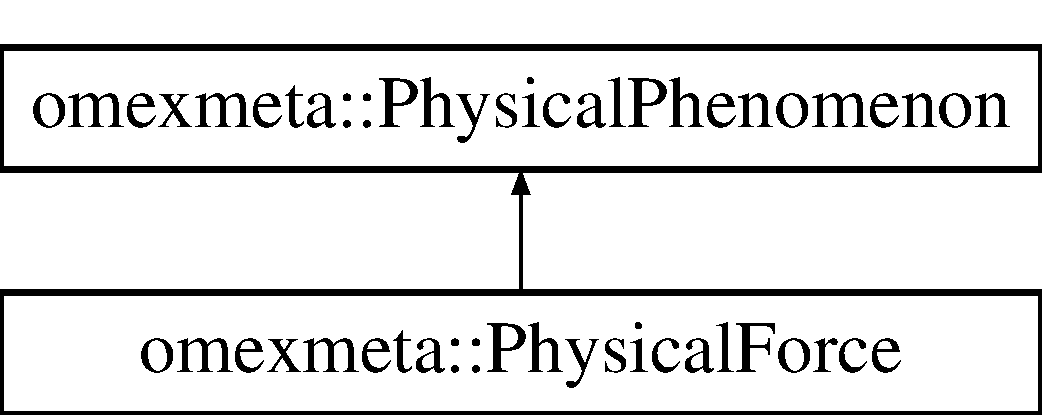
\includegraphics[height=2.000000cm]{classomexmeta_1_1PhysicalForce}
\end{center}
\end{figure}
\subsection*{Public Member Functions}
\begin{DoxyCompactItemize}
\item 
\hyperlink{classomexmeta_1_1PhysicalForce_ad5b43ea5489891c45f5ebc4c9b62e44e}{Physical\+Force} ()=delete
\begin{DoxyCompactList}\small\item\em default constructor for \hyperlink{classomexmeta_1_1PhysicalForce}{Physical\+Force} \end{DoxyCompactList}\item 
\mbox{\Hypertarget{classomexmeta_1_1PhysicalForce_a8761d703a67c6dc81b4a71b90391b20f}\label{classomexmeta_1_1PhysicalForce_a8761d703a67c6dc81b4a71b90391b20f}} 
{\bfseries Physical\+Force} (librdf\+\_\+model $\ast$model, std\+::string model\+\_\+uri, std\+::string local\+\_\+uri, \hyperlink{classomexmeta_1_1PhysicalProperty}{Physical\+Property} physical\+Property, Sources sources, Sinks sinks)
\item 
void \hyperlink{classomexmeta_1_1PhysicalForce_a41cd6c9904f3287bb8cbbab2b9d2ada3}{free} ()
\begin{DoxyCompactList}\small\item\em Free nodes associated with \hyperlink{classomexmeta_1_1PhysicalForce}{Physical\+Force}. \end{DoxyCompactList}\item 
\hyperlink{classomexmeta_1_1PhysicalForce_a673e6810fe969bcd087ab88c62e5e041}{Physical\+Force} (librdf\+\_\+model $\ast$model)
\begin{DoxyCompactList}\small\item\em constructor for instantiating a \hyperlink{classomexmeta_1_1PhysicalForce}{Physical\+Force} type composite annotation \end{DoxyCompactList}\item 
\hyperlink{classomexmeta_1_1PhysicalForce_a2ff9aecd73a5356be701d8ba7e9bf71c}{Physical\+Force} (librdf\+\_\+model $\ast$model, const std\+::string \&model\+\_\+uri, const std\+::string \&local\+\_\+uri)
\begin{DoxyCompactList}\small\item\em constructor for instantiating a \hyperlink{classomexmeta_1_1PhysicalForce}{Physical\+Force} type composite annotation \end{DoxyCompactList}\item 
std\+::string \hyperlink{classomexmeta_1_1PhysicalForce_ae0a9ec4689b4765d985ab8f7a8878f38}{create\+Meta\+Id} ()
\begin{DoxyCompactList}\small\item\em create a metaid for the physical force annotation \end{DoxyCompactList}\item 
const Sources \& \hyperlink{classomexmeta_1_1PhysicalForce_aa42b8e04573d2ae88f952c76b146d5ac}{get\+Sources} () const
\begin{DoxyCompactList}\small\item\em return vector of Source objects assocated with \hyperlink{classomexmeta_1_1PhysicalForce}{Physical\+Force} \end{DoxyCompactList}\item 
const Sinks \& \hyperlink{classomexmeta_1_1PhysicalForce_ab37bbe3a0f762066fdb43e5c2ce608eb}{get\+Sinks} () const
\begin{DoxyCompactList}\small\item\em return vector of Sink objects assocated with \hyperlink{classomexmeta_1_1PhysicalForce}{Physical\+Force} \end{DoxyCompactList}\item 
\hyperlink{classomexmeta_1_1Triples}{Triples} \hyperlink{classomexmeta_1_1PhysicalForce_a39dd511aee85130d07cb6ffb3f8e87f0}{to\+Triples} () override
\begin{DoxyCompactList}\small\item\em converts the Phyical\+Force object into a \hyperlink{classomexmeta_1_1Triples}{Triples} object. \end{DoxyCompactList}\item 
\hyperlink{classomexmeta_1_1PhysicalForce}{Physical\+Force} \& \hyperlink{classomexmeta_1_1PhysicalForce_a081aecc43d16b2fc8826c4050eb2055d}{set\+Physical\+Property} (\hyperlink{classomexmeta_1_1PhysicalProperty}{Physical\+Property} physical\+Property)
\begin{DoxyCompactList}\small\item\em sets the physical property of the \hyperlink{classomexmeta_1_1PhysicalForce}{Physical\+Force}  physical\+Property An instance of \hyperlink{classomexmeta_1_1PhysicalProperty}{Physical\+Property} representing the physical property term for the \hyperlink{classomexmeta_1_1PhysicalForce}{Physical\+Force}. \end{DoxyCompactList}\item 
\hyperlink{classomexmeta_1_1PhysicalForce}{Physical\+Force} \& \hyperlink{classomexmeta_1_1PhysicalForce_a3f979432322d40efc8a15cf5ee883100}{set\+Physical\+Property} (std\+::string subject\+\_\+metaid, std\+::string physical\+\_\+property)
\begin{DoxyCompactList}\small\item\em sets the physical property of the \hyperlink{classomexmeta_1_1PhysicalForce}{Physical\+Force} \end{DoxyCompactList}\item 
\hyperlink{classomexmeta_1_1PhysicalForce}{Physical\+Force} \& \hyperlink{classomexmeta_1_1PhysicalForce_ace7d3703d7e4bdb9a256208f456f2c4f}{add\+Source} (int multiplier, const std\+::string \&physical\+\_\+entity\+\_\+reference)
\begin{DoxyCompactList}\small\item\em add a \hyperlink{classomexmeta_1_1SourceParticipant}{Source\+Participant} to the \hyperlink{classomexmeta_1_1PhysicalForce}{Physical\+Force}. \end{DoxyCompactList}\item 
\hyperlink{classomexmeta_1_1PhysicalForce}{Physical\+Force} \& \hyperlink{classomexmeta_1_1PhysicalForce_a8ec5e262b82526ac914d8c7f10b6c2f1}{add\+Sink} (int multiplier, const std\+::string \&physical\+\_\+entity\+\_\+reference)
\begin{DoxyCompactList}\small\item\em add a \hyperlink{classomexmeta_1_1SinkParticipant}{Sink\+Participant} to the \hyperlink{classomexmeta_1_1PhysicalForce}{Physical\+Force}. \end{DoxyCompactList}\item 
int \hyperlink{classomexmeta_1_1PhysicalForce_a9910c8edac57daf70faa1f1e2e0208d1}{get\+Num\+Sources} ()
\begin{DoxyCompactList}\small\item\em returns the number of sources associated with the \hyperlink{classomexmeta_1_1PhysicalForce}{Physical\+Force} \end{DoxyCompactList}\item 
int \hyperlink{classomexmeta_1_1PhysicalForce_a1135c75705b59afa7037bab313009534}{get\+Num\+Sinks} ()
\begin{DoxyCompactList}\small\item\em returns the number of sinks associated with the \hyperlink{classomexmeta_1_1PhysicalForce}{Physical\+Force} \end{DoxyCompactList}\item 
\mbox{\Hypertarget{classomexmeta_1_1PhysicalForce_affa0a1f3cdce0a3336d56658a92c65f3}\label{classomexmeta_1_1PhysicalForce_affa0a1f3cdce0a3336d56658a92c65f3}} 
bool {\bfseries operator==} (const \hyperlink{classomexmeta_1_1PhysicalForce}{Physical\+Force} \&rhs) const
\item 
\mbox{\Hypertarget{classomexmeta_1_1PhysicalForce_aeb7adb235c0caac04c7aa599f98f258a}\label{classomexmeta_1_1PhysicalForce_aeb7adb235c0caac04c7aa599f98f258a}} 
bool {\bfseries operator!=} (const \hyperlink{classomexmeta_1_1PhysicalForce}{Physical\+Force} \&rhs) const
\end{DoxyCompactItemize}
\subsection*{Additional Inherited Members}


\subsection{Constructor \& Destructor Documentation}
\mbox{\Hypertarget{classomexmeta_1_1PhysicalForce_ad5b43ea5489891c45f5ebc4c9b62e44e}\label{classomexmeta_1_1PhysicalForce_ad5b43ea5489891c45f5ebc4c9b62e44e}} 
\index{omexmeta\+::\+Physical\+Force@{omexmeta\+::\+Physical\+Force}!Physical\+Force@{Physical\+Force}}
\index{Physical\+Force@{Physical\+Force}!omexmeta\+::\+Physical\+Force@{omexmeta\+::\+Physical\+Force}}
\subsubsection{\texorpdfstring{Physical\+Force()}{PhysicalForce()}\hspace{0.1cm}{\footnotesize\ttfamily [1/3]}}
{\footnotesize\ttfamily omexmeta\+::\+Physical\+Force\+::\+Physical\+Force (\begin{DoxyParamCaption}{ }\end{DoxyParamCaption})\hspace{0.3cm}{\ttfamily [delete]}}



default constructor for \hyperlink{classomexmeta_1_1PhysicalForce}{Physical\+Force} 

deliberately deleted. If you try using the builder interface (chaining setter methods) from a default instantiated \hyperlink{classomexmeta_1_1PhysicalForce}{Physical\+Force} you will get an error, because there will be no model assicated with \hyperlink{classomexmeta_1_1PhysicalForce}{Physical\+Force}. Instead, always instantiate a \hyperlink{classomexmeta_1_1PhysicalForce}{Physical\+Force} from the \hyperlink{classomexmeta_1_1Editor_a7833e03995f6323109c2db8d59104f6c}{Editor\+::add\+Physical\+Force()} method. \mbox{\Hypertarget{classomexmeta_1_1PhysicalForce_a673e6810fe969bcd087ab88c62e5e041}\label{classomexmeta_1_1PhysicalForce_a673e6810fe969bcd087ab88c62e5e041}} 
\index{omexmeta\+::\+Physical\+Force@{omexmeta\+::\+Physical\+Force}!Physical\+Force@{Physical\+Force}}
\index{Physical\+Force@{Physical\+Force}!omexmeta\+::\+Physical\+Force@{omexmeta\+::\+Physical\+Force}}
\subsubsection{\texorpdfstring{Physical\+Force()}{PhysicalForce()}\hspace{0.1cm}{\footnotesize\ttfamily [2/3]}}
{\footnotesize\ttfamily omexmeta\+::\+Physical\+Force\+::\+Physical\+Force (\begin{DoxyParamCaption}\item[{librdf\+\_\+model $\ast$}]{model }\end{DoxyParamCaption})\hspace{0.3cm}{\ttfamily [explicit]}}



constructor for instantiating a \hyperlink{classomexmeta_1_1PhysicalForce}{Physical\+Force} type composite annotation 


\begin{DoxyParams}{Parameters}
{\em model.} & A librdf\+\_\+model pass down by \hyperlink{classomexmeta_1_1Editor}{Editor}.\\
\hline
\end{DoxyParams}
Users do not need to instantiate \hyperlink{classomexmeta_1_1PhysicalForce}{Physical\+Force} manually, since it is done by \hyperlink{classomexmeta_1_1Editor}{Editor}. \hyperlink{classThis}{This} constructor instantiates an empty \hyperlink{classomexmeta_1_1PhysicalForce}{Physical\+Force} object which is filled by \mbox{\Hypertarget{classomexmeta_1_1PhysicalForce_a2ff9aecd73a5356be701d8ba7e9bf71c}\label{classomexmeta_1_1PhysicalForce_a2ff9aecd73a5356be701d8ba7e9bf71c}} 
\index{omexmeta\+::\+Physical\+Force@{omexmeta\+::\+Physical\+Force}!Physical\+Force@{Physical\+Force}}
\index{Physical\+Force@{Physical\+Force}!omexmeta\+::\+Physical\+Force@{omexmeta\+::\+Physical\+Force}}
\subsubsection{\texorpdfstring{Physical\+Force()}{PhysicalForce()}\hspace{0.1cm}{\footnotesize\ttfamily [3/3]}}
{\footnotesize\ttfamily omexmeta\+::\+Physical\+Force\+::\+Physical\+Force (\begin{DoxyParamCaption}\item[{librdf\+\_\+model $\ast$}]{model,  }\item[{const std\+::string \&}]{model\+\_\+uri,  }\item[{const std\+::string \&}]{local\+\_\+uri }\end{DoxyParamCaption})\hspace{0.3cm}{\ttfamily [explicit]}}



constructor for instantiating a \hyperlink{classomexmeta_1_1PhysicalForce}{Physical\+Force} type composite annotation 


\begin{DoxyParams}{Parameters}
{\em model.} & A librdf\+\_\+model pass down by \hyperlink{classomexmeta_1_1Editor}{Editor}. \\
\hline
{\em model\+\_\+uri.} & String passed down by \hyperlink{classomexmeta_1_1Editor}{Editor}. The local uri to use for metaids\\
\hline
\end{DoxyParams}
Users do not need to instantiate \hyperlink{classomexmeta_1_1PhysicalForce}{Physical\+Force} manually, since it is done by \hyperlink{classomexmeta_1_1Editor}{Editor}. \hyperlink{classThis}{This} constructor instantiates an empty \hyperlink{classomexmeta_1_1PhysicalForce}{Physical\+Force} object which is filled by 

\subsection{Member Function Documentation}
\mbox{\Hypertarget{classomexmeta_1_1PhysicalForce_a8ec5e262b82526ac914d8c7f10b6c2f1}\label{classomexmeta_1_1PhysicalForce_a8ec5e262b82526ac914d8c7f10b6c2f1}} 
\index{omexmeta\+::\+Physical\+Force@{omexmeta\+::\+Physical\+Force}!add\+Sink@{add\+Sink}}
\index{add\+Sink@{add\+Sink}!omexmeta\+::\+Physical\+Force@{omexmeta\+::\+Physical\+Force}}
\subsubsection{\texorpdfstring{add\+Sink()}{addSink()}}
{\footnotesize\ttfamily \hyperlink{classomexmeta_1_1PhysicalForce}{Physical\+Force} \& omexmeta\+::\+Physical\+Force\+::add\+Sink (\begin{DoxyParamCaption}\item[{int}]{multiplier,  }\item[{const std\+::string \&}]{physical\+\_\+entity\+\_\+reference }\end{DoxyParamCaption})}



add a \hyperlink{classomexmeta_1_1SinkParticipant}{Sink\+Participant} to the \hyperlink{classomexmeta_1_1PhysicalForce}{Physical\+Force}. 


\begin{DoxyParams}{Parameters}
{\em sink\+\_\+metaid} & the ID for the \hyperlink{classomexmeta_1_1SinkParticipant}{Sink\+Participant}. \\
\hline
{\em multiplier} & The multiplier argument for \hyperlink{classomexmeta_1_1SinkParticipant}{Sink\+Participant} \\
\hline
{\em physical\+\_\+entity\+\_\+reference} & The physical\+Entity\+Reference argument for the \hyperlink{classomexmeta_1_1SinkParticipant}{Sink\+Participant}. \\
\hline
\end{DoxyParams}
\begin{DoxyReturn}{Returns}
a reference to this \hyperlink{classomexmeta_1_1PhysicalForce}{Physical\+Force} to enable the builder interface.
\end{DoxyReturn}
See \hyperlink{classomexmeta_1_1SinkParticipant}{Sink\+Participant} documentation for more details on arguments. \mbox{\Hypertarget{classomexmeta_1_1PhysicalForce_ace7d3703d7e4bdb9a256208f456f2c4f}\label{classomexmeta_1_1PhysicalForce_ace7d3703d7e4bdb9a256208f456f2c4f}} 
\index{omexmeta\+::\+Physical\+Force@{omexmeta\+::\+Physical\+Force}!add\+Source@{add\+Source}}
\index{add\+Source@{add\+Source}!omexmeta\+::\+Physical\+Force@{omexmeta\+::\+Physical\+Force}}
\subsubsection{\texorpdfstring{add\+Source()}{addSource()}}
{\footnotesize\ttfamily \hyperlink{classomexmeta_1_1PhysicalForce}{Physical\+Force} \& omexmeta\+::\+Physical\+Force\+::add\+Source (\begin{DoxyParamCaption}\item[{int}]{multiplier,  }\item[{const std\+::string \&}]{physical\+\_\+entity\+\_\+reference }\end{DoxyParamCaption})}



add a \hyperlink{classomexmeta_1_1SourceParticipant}{Source\+Participant} to the \hyperlink{classomexmeta_1_1PhysicalForce}{Physical\+Force}. 


\begin{DoxyParams}{Parameters}
{\em metaid} & the ID for the \hyperlink{classomexmeta_1_1SourceParticipant}{Source\+Participant}. \\
\hline
{\em multiplier} & The multiplier argument for \hyperlink{classomexmeta_1_1SourceParticipant}{Source\+Participant} \\
\hline
{\em physical\+\_\+entity\+\_\+reference} & The physical\+Entity\+Reference argument for the \hyperlink{classomexmeta_1_1SourceParticipant}{Source\+Participant}. \\
\hline
\end{DoxyParams}
\begin{DoxyReturn}{Returns}
a reference to this \hyperlink{classomexmeta_1_1PhysicalForce}{Physical\+Force} to enable the builder interface.
\end{DoxyReturn}
See \hyperlink{classomexmeta_1_1SourceParticipant}{Source\+Participant} documentation for more details on arguments. \mbox{\Hypertarget{classomexmeta_1_1PhysicalForce_ae0a9ec4689b4765d985ab8f7a8878f38}\label{classomexmeta_1_1PhysicalForce_ae0a9ec4689b4765d985ab8f7a8878f38}} 
\index{omexmeta\+::\+Physical\+Force@{omexmeta\+::\+Physical\+Force}!create\+Meta\+Id@{create\+Meta\+Id}}
\index{create\+Meta\+Id@{create\+Meta\+Id}!omexmeta\+::\+Physical\+Force@{omexmeta\+::\+Physical\+Force}}
\subsubsection{\texorpdfstring{create\+Meta\+Id()}{createMetaId()}}
{\footnotesize\ttfamily std\+::string omexmeta\+::\+Physical\+Force\+::create\+Meta\+Id (\begin{DoxyParamCaption}{ }\end{DoxyParamCaption})}



create a metaid for the physical force annotation 

a new metaid for \hyperlink{classomexmeta_1_1PhysicalForce}{Physical\+Force} \mbox{\Hypertarget{classomexmeta_1_1PhysicalForce_a41cd6c9904f3287bb8cbbab2b9d2ada3}\label{classomexmeta_1_1PhysicalForce_a41cd6c9904f3287bb8cbbab2b9d2ada3}} 
\index{omexmeta\+::\+Physical\+Force@{omexmeta\+::\+Physical\+Force}!free@{free}}
\index{free@{free}!omexmeta\+::\+Physical\+Force@{omexmeta\+::\+Physical\+Force}}
\subsubsection{\texorpdfstring{free()}{free()}}
{\footnotesize\ttfamily void omexmeta\+::\+Physical\+Force\+::free (\begin{DoxyParamCaption}{ }\end{DoxyParamCaption})}



Free nodes associated with \hyperlink{classomexmeta_1_1PhysicalForce}{Physical\+Force}. 

The \hyperlink{classomexmeta_1_1PhysicalForce}{Physical\+Force} is owned by the caller if the \hyperlink{classomexmeta_1_1PhysicalForce_a39dd511aee85130d07cb6ffb3f8e87f0}{Physical\+Force\+::to\+Triples} method is N\+OT used. When \hyperlink{classomexmeta_1_1PhysicalForce_a39dd511aee85130d07cb6ffb3f8e87f0}{to\+Triples()} is used, the nodes that create the \hyperlink{classomexmeta_1_1PhysicalForce}{Physical\+Force} are \char`\"{}given\char`\"{} to the \hyperlink{classomexmeta_1_1Triples}{Triples} object, which automatically destroys them at the right time.

Most of the time, users will not have to remember to free the \hyperlink{classomexmeta_1_1PhysicalForce}{Physical\+Force} themselves as the to\+Triples method is always used. \mbox{\Hypertarget{classomexmeta_1_1PhysicalForce_a1135c75705b59afa7037bab313009534}\label{classomexmeta_1_1PhysicalForce_a1135c75705b59afa7037bab313009534}} 
\index{omexmeta\+::\+Physical\+Force@{omexmeta\+::\+Physical\+Force}!get\+Num\+Sinks@{get\+Num\+Sinks}}
\index{get\+Num\+Sinks@{get\+Num\+Sinks}!omexmeta\+::\+Physical\+Force@{omexmeta\+::\+Physical\+Force}}
\subsubsection{\texorpdfstring{get\+Num\+Sinks()}{getNumSinks()}}
{\footnotesize\ttfamily int omexmeta\+::\+Physical\+Force\+::get\+Num\+Sinks (\begin{DoxyParamCaption}{ }\end{DoxyParamCaption})}



returns the number of sinks associated with the \hyperlink{classomexmeta_1_1PhysicalForce}{Physical\+Force} 

\begin{DoxyReturn}{Returns}
the integer number of sinks 
\end{DoxyReturn}
\mbox{\Hypertarget{classomexmeta_1_1PhysicalForce_a9910c8edac57daf70faa1f1e2e0208d1}\label{classomexmeta_1_1PhysicalForce_a9910c8edac57daf70faa1f1e2e0208d1}} 
\index{omexmeta\+::\+Physical\+Force@{omexmeta\+::\+Physical\+Force}!get\+Num\+Sources@{get\+Num\+Sources}}
\index{get\+Num\+Sources@{get\+Num\+Sources}!omexmeta\+::\+Physical\+Force@{omexmeta\+::\+Physical\+Force}}
\subsubsection{\texorpdfstring{get\+Num\+Sources()}{getNumSources()}}
{\footnotesize\ttfamily int omexmeta\+::\+Physical\+Force\+::get\+Num\+Sources (\begin{DoxyParamCaption}{ }\end{DoxyParamCaption})}



returns the number of sources associated with the \hyperlink{classomexmeta_1_1PhysicalForce}{Physical\+Force} 

\begin{DoxyReturn}{Returns}
the integer number of sources 
\end{DoxyReturn}
\mbox{\Hypertarget{classomexmeta_1_1PhysicalForce_ab37bbe3a0f762066fdb43e5c2ce608eb}\label{classomexmeta_1_1PhysicalForce_ab37bbe3a0f762066fdb43e5c2ce608eb}} 
\index{omexmeta\+::\+Physical\+Force@{omexmeta\+::\+Physical\+Force}!get\+Sinks@{get\+Sinks}}
\index{get\+Sinks@{get\+Sinks}!omexmeta\+::\+Physical\+Force@{omexmeta\+::\+Physical\+Force}}
\subsubsection{\texorpdfstring{get\+Sinks()}{getSinks()}}
{\footnotesize\ttfamily const std\+::vector$<$ \hyperlink{classomexmeta_1_1SinkParticipant}{Sink\+Participant} $>$ \& omexmeta\+::\+Physical\+Force\+::get\+Sinks (\begin{DoxyParamCaption}{ }\end{DoxyParamCaption}) const}



return vector of Sink objects assocated with \hyperlink{classomexmeta_1_1PhysicalForce}{Physical\+Force} 

\begin{DoxyReturn}{Returns}
a vector of Sink\+Participants 
\end{DoxyReturn}
\mbox{\Hypertarget{classomexmeta_1_1PhysicalForce_aa42b8e04573d2ae88f952c76b146d5ac}\label{classomexmeta_1_1PhysicalForce_aa42b8e04573d2ae88f952c76b146d5ac}} 
\index{omexmeta\+::\+Physical\+Force@{omexmeta\+::\+Physical\+Force}!get\+Sources@{get\+Sources}}
\index{get\+Sources@{get\+Sources}!omexmeta\+::\+Physical\+Force@{omexmeta\+::\+Physical\+Force}}
\subsubsection{\texorpdfstring{get\+Sources()}{getSources()}}
{\footnotesize\ttfamily const std\+::vector$<$ \hyperlink{classomexmeta_1_1SourceParticipant}{Source\+Participant} $>$ \& omexmeta\+::\+Physical\+Force\+::get\+Sources (\begin{DoxyParamCaption}{ }\end{DoxyParamCaption}) const}



return vector of Source objects assocated with \hyperlink{classomexmeta_1_1PhysicalForce}{Physical\+Force} 

\begin{DoxyReturn}{Returns}
a vector of Source\+Participants 
\end{DoxyReturn}
\mbox{\Hypertarget{classomexmeta_1_1PhysicalForce_a081aecc43d16b2fc8826c4050eb2055d}\label{classomexmeta_1_1PhysicalForce_a081aecc43d16b2fc8826c4050eb2055d}} 
\index{omexmeta\+::\+Physical\+Force@{omexmeta\+::\+Physical\+Force}!set\+Physical\+Property@{set\+Physical\+Property}}
\index{set\+Physical\+Property@{set\+Physical\+Property}!omexmeta\+::\+Physical\+Force@{omexmeta\+::\+Physical\+Force}}
\subsubsection{\texorpdfstring{set\+Physical\+Property()}{setPhysicalProperty()}\hspace{0.1cm}{\footnotesize\ttfamily [1/2]}}
{\footnotesize\ttfamily \hyperlink{classomexmeta_1_1PhysicalForce}{Physical\+Force} \& omexmeta\+::\+Physical\+Force\+::set\+Physical\+Property (\begin{DoxyParamCaption}\item[{\hyperlink{classomexmeta_1_1PhysicalProperty}{Physical\+Property}}]{physical\+Property }\end{DoxyParamCaption})}



sets the physical property of the \hyperlink{classomexmeta_1_1PhysicalForce}{Physical\+Force}  physical\+Property An instance of \hyperlink{classomexmeta_1_1PhysicalProperty}{Physical\+Property} representing the physical property term for the \hyperlink{classomexmeta_1_1PhysicalForce}{Physical\+Force}. 

\begin{DoxyReturn}{Returns}
a reference to this \hyperlink{classomexmeta_1_1PhysicalForce}{Physical\+Force} to enable the builder interface.
\end{DoxyReturn}
Prefer the other set\+Physical\+Property method since it only requires a string input and instantiates the \hyperlink{classomexmeta_1_1PhysicalProperty}{Physical\+Property} for you.

For developers. Consider removing. \mbox{\Hypertarget{classomexmeta_1_1PhysicalForce_a3f979432322d40efc8a15cf5ee883100}\label{classomexmeta_1_1PhysicalForce_a3f979432322d40efc8a15cf5ee883100}} 
\index{omexmeta\+::\+Physical\+Force@{omexmeta\+::\+Physical\+Force}!set\+Physical\+Property@{set\+Physical\+Property}}
\index{set\+Physical\+Property@{set\+Physical\+Property}!omexmeta\+::\+Physical\+Force@{omexmeta\+::\+Physical\+Force}}
\subsubsection{\texorpdfstring{set\+Physical\+Property()}{setPhysicalProperty()}\hspace{0.1cm}{\footnotesize\ttfamily [2/2]}}
{\footnotesize\ttfamily \hyperlink{classomexmeta_1_1PhysicalForce}{Physical\+Force} \& omexmeta\+::\+Physical\+Force\+::set\+Physical\+Property (\begin{DoxyParamCaption}\item[{std\+::string}]{subject\+\_\+metaid,  }\item[{std\+::string}]{physical\+\_\+property }\end{DoxyParamCaption})}



sets the physical property of the \hyperlink{classomexmeta_1_1PhysicalForce}{Physical\+Force} 


\begin{DoxyParams}{Parameters}
{\em subject\+\_\+metaid.} & The subject portion of the two triples produced by \hyperlink{classomexmeta_1_1PhysicalProperty}{Physical\+Property}. Metaid of a model element. \\
\hline
{\em A} & string representing the O\+PB term to use as the physical property. Like \char`\"{}\+O\+P\+B\+:\+O\+P\+B\+\_\+1234\char`\"{} \\
\hline
\end{DoxyParams}
\begin{DoxyReturn}{Returns}
a reference to this \hyperlink{classomexmeta_1_1PhysicalForce}{Physical\+Force} to enable the builder interface. 
\end{DoxyReturn}
\mbox{\Hypertarget{classomexmeta_1_1PhysicalForce_a39dd511aee85130d07cb6ffb3f8e87f0}\label{classomexmeta_1_1PhysicalForce_a39dd511aee85130d07cb6ffb3f8e87f0}} 
\index{omexmeta\+::\+Physical\+Force@{omexmeta\+::\+Physical\+Force}!to\+Triples@{to\+Triples}}
\index{to\+Triples@{to\+Triples}!omexmeta\+::\+Physical\+Force@{omexmeta\+::\+Physical\+Force}}
\subsubsection{\texorpdfstring{to\+Triples()}{toTriples()}}
{\footnotesize\ttfamily \hyperlink{classomexmeta_1_1Triples}{Triples} omexmeta\+::\+Physical\+Force\+::to\+Triples (\begin{DoxyParamCaption}{ }\end{DoxyParamCaption})\hspace{0.3cm}{\ttfamily [override]}, {\ttfamily [virtual]}}



converts the Phyical\+Force object into a \hyperlink{classomexmeta_1_1Triples}{Triples} object. 

\begin{DoxyReturn}{Returns}
a \hyperlink{classomexmeta_1_1Triples}{Triples} object containing the individual \hyperlink{classomexmeta_1_1Triple}{Triple} objects of a \hyperlink{classomexmeta_1_1PhysicalForce}{Physical\+Force}.
\end{DoxyReturn}
When this method is called ownership of all \hyperlink{classomexmeta_1_1RDF}{R\+DF} nodes gets transferred from the caller to the returned \hyperlink{classomexmeta_1_1Triples}{Triples} object. 

Reimplemented from \hyperlink{classomexmeta_1_1PhysicalPhenomenon_a30617e685bd8b155a76d38ab5a9db273}{omexmeta\+::\+Physical\+Phenomenon}.



The documentation for this class was generated from the following files\+:\begin{DoxyCompactItemize}
\item 
src/omexmeta/Physical\+Force.\+h\item 
src/omexmeta/Physical\+Force.\+cpp\end{DoxyCompactItemize}

\hypertarget{classomexmeta_1_1PhysicalPhenomenon}{}\doxysection{omexmeta\+::Physical\+Phenomenon Class Reference}
\label{classomexmeta_1_1PhysicalPhenomenon}\index{omexmeta::PhysicalPhenomenon@{omexmeta::PhysicalPhenomenon}}
Inheritance diagram for omexmeta\+::Physical\+Phenomenon\+:\begin{figure}[H]
\begin{center}
\leavevmode
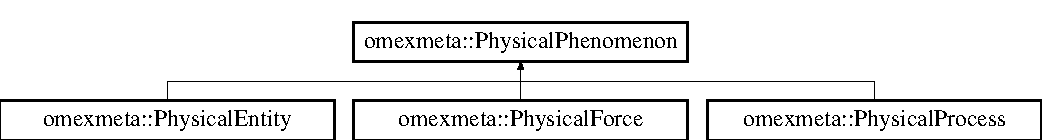
\includegraphics[height=1.848185cm]{classomexmeta_1_1PhysicalPhenomenon}
\end{center}
\end{figure}
\doxysubsection*{Public Member Functions}
\begin{DoxyCompactItemize}
\item 
\mbox{\Hypertarget{classomexmeta_1_1PhysicalPhenomenon_a1c3322453b3c6831668ffa98d9f4b6af}\label{classomexmeta_1_1PhysicalPhenomenon_a1c3322453b3c6831668ffa98d9f4b6af}} 
bool {\bfseries operator==} (const \mbox{\hyperlink{classomexmeta_1_1PhysicalPhenomenon}{Physical\+Phenomenon}} \&rhs) const
\item 
\mbox{\Hypertarget{classomexmeta_1_1PhysicalPhenomenon_a2c726263714e31c7c19d6e73c2c593f8}\label{classomexmeta_1_1PhysicalPhenomenon_a2c726263714e31c7c19d6e73c2c593f8}} 
bool {\bfseries operator!=} (const \mbox{\hyperlink{classomexmeta_1_1PhysicalPhenomenon}{Physical\+Phenomenon}} \&rhs) const
\item 
\mbox{\Hypertarget{classomexmeta_1_1PhysicalPhenomenon_a2d59ebbc920a40348d102af31ed6661a}\label{classomexmeta_1_1PhysicalPhenomenon_a2d59ebbc920a40348d102af31ed6661a}} 
const std\+::string \& {\bfseries get\+Local\+Uri} () const
\item 
\mbox{\Hypertarget{classomexmeta_1_1PhysicalPhenomenon_a84cae9aa96ca00df45b0f81dd8d3ffd4}\label{classomexmeta_1_1PhysicalPhenomenon_a84cae9aa96ca00df45b0f81dd8d3ffd4}} 
void {\bfseries set\+Local\+Uri} (const std\+::string \&local\+Uri)
\item 
\mbox{\Hypertarget{classomexmeta_1_1PhysicalPhenomenon_ad823dad75504adb78975c810e5f1ff94}\label{classomexmeta_1_1PhysicalPhenomenon_ad823dad75504adb78975c810e5f1ff94}} 
\mbox{\hyperlink{classomexmeta_1_1PhysicalPhenomenon_ad823dad75504adb78975c810e5f1ff94}{Physical\+Phenomenon}} (const \mbox{\hyperlink{classomexmeta_1_1PhysicalPhenomenon}{Physical\+Phenomenon}} \&phenomenon)=delete
\begin{DoxyCompactList}\small\item\em Copy constructor for \mbox{\hyperlink{classomexmeta_1_1PhysicalPhenomenon}{Physical\+Phenomenon}}. \end{DoxyCompactList}\item 
\mbox{\Hypertarget{classomexmeta_1_1PhysicalPhenomenon_aeb95aedf1756ded154ec6753108a691e}\label{classomexmeta_1_1PhysicalPhenomenon_aeb95aedf1756ded154ec6753108a691e}} 
\mbox{\hyperlink{classomexmeta_1_1PhysicalPhenomenon_aeb95aedf1756ded154ec6753108a691e}{Physical\+Phenomenon}} (\mbox{\hyperlink{classomexmeta_1_1PhysicalPhenomenon}{Physical\+Phenomenon}} \&\&phenomenon) noexcept
\begin{DoxyCompactList}\small\item\em Move constructor for \mbox{\hyperlink{classomexmeta_1_1PhysicalPhenomenon}{Physical\+Phenomenon}}. \end{DoxyCompactList}\item 
\mbox{\Hypertarget{classomexmeta_1_1PhysicalPhenomenon_aac3920bfe9bf16e071ebdd8ed4fabe2f}\label{classomexmeta_1_1PhysicalPhenomenon_aac3920bfe9bf16e071ebdd8ed4fabe2f}} 
\mbox{\hyperlink{classomexmeta_1_1PhysicalPhenomenon}{Physical\+Phenomenon}} \& \mbox{\hyperlink{classomexmeta_1_1PhysicalPhenomenon_aac3920bfe9bf16e071ebdd8ed4fabe2f}{operator=}} (const \mbox{\hyperlink{classomexmeta_1_1PhysicalPhenomenon}{Physical\+Phenomenon}} \&phenomenon)=delete
\begin{DoxyCompactList}\small\item\em assignment operator for \mbox{\hyperlink{classomexmeta_1_1PhysicalPhenomenon}{Physical\+Phenomenon}} \end{DoxyCompactList}\item 
\mbox{\Hypertarget{classomexmeta_1_1PhysicalPhenomenon_af15355b4c2a361b4b02dca02d3877aed}\label{classomexmeta_1_1PhysicalPhenomenon_af15355b4c2a361b4b02dca02d3877aed}} 
\mbox{\hyperlink{classomexmeta_1_1PhysicalPhenomenon}{Physical\+Phenomenon}} \& \mbox{\hyperlink{classomexmeta_1_1PhysicalPhenomenon_af15355b4c2a361b4b02dca02d3877aed}{operator=}} (\mbox{\hyperlink{classomexmeta_1_1PhysicalPhenomenon}{Physical\+Phenomenon}} \&\&phenomenon) noexcept
\begin{DoxyCompactList}\small\item\em move assignment operator for \mbox{\hyperlink{classomexmeta_1_1PhysicalPhenomenon}{Physical\+Phenomenon}} \end{DoxyCompactList}\item 
\mbox{\hyperlink{classomexmeta_1_1PhysicalPhenomenon_aa140516da97b03960175f9bc04ecf865}{Physical\+Phenomenon}} (librdf\+\_\+model $\ast$model)
\begin{DoxyCompactList}\small\item\em Constructor for builder interface. \end{DoxyCompactList}\item 
\mbox{\hyperlink{classomexmeta_1_1PhysicalPhenomenon_a5c831ca76c36121b0fbc7b122b5539ac}{Physical\+Phenomenon}} (librdf\+\_\+model $\ast$model, std\+::string model\+\_\+uri, std\+::string local\+\_\+uri)
\begin{DoxyCompactList}\small\item\em Constructor for builder interface. \end{DoxyCompactList}\item 
\mbox{\hyperlink{classomexmeta_1_1PhysicalPhenomenon_a93bf263f7fdb65bd3e8de97983a7186b}{Physical\+Phenomenon}} (librdf\+\_\+model $\ast$model, std\+::string model\+\_\+uri, std\+::string local\+\_\+uri, \mbox{\hyperlink{classomexmeta_1_1PhysicalProperty}{Physical\+Property}} property\+Resource, \mbox{\hyperlink{namespaceomexmeta_a1129ebb8a92218ebb27b9c76ac8462f7}{Annotation\+Type}} type)
\begin{DoxyCompactList}\small\item\em constructor for \mbox{\hyperlink{classomexmeta_1_1PhysicalPhenomenon}{Physical\+Phenomenon}} object. \end{DoxyCompactList}\item 
\mbox{\Hypertarget{classomexmeta_1_1PhysicalPhenomenon_a5528b12e5dbc702c0c270328662e7031}\label{classomexmeta_1_1PhysicalPhenomenon_a5528b12e5dbc702c0c270328662e7031}} 
const std\+::string \& {\bfseries get\+Model\+Uri} () const
\item 
\mbox{\Hypertarget{classomexmeta_1_1PhysicalPhenomenon_aa1fd9929fb2e07fa20081b1a4c00c9d2}\label{classomexmeta_1_1PhysicalPhenomenon_aa1fd9929fb2e07fa20081b1a4c00c9d2}} 
void {\bfseries set\+Model\+Uri} (const std\+::string \&model\+Uri)
\item 
const std\+::string \& \mbox{\hyperlink{classomexmeta_1_1PhysicalPhenomenon_a8be912d1256d6b913c4965f96f1b730b}{get\+About}} () const
\begin{DoxyCompactList}\small\item\em get the subject portion of the \mbox{\hyperlink{classomexmeta_1_1PhysicalPhenomenon}{Physical\+Phenomenon}} \end{DoxyCompactList}\item 
const std\+::string \& \mbox{\hyperlink{classomexmeta_1_1PhysicalPhenomenon_aa09896afed6124d042d7d8f82b21cae9}{set\+About}} () const
\begin{DoxyCompactList}\small\item\em set the subject portion of the \mbox{\hyperlink{classomexmeta_1_1PhysicalPhenomenon}{Physical\+Phenomenon}} \end{DoxyCompactList}\item 
\mbox{\hyperlink{namespaceomexmeta_a1129ebb8a92218ebb27b9c76ac8462f7}{Annotation\+Type}} \mbox{\hyperlink{classomexmeta_1_1PhysicalPhenomenon_a9676a1dcc458247a19d19cda16d640f4}{get\+Type}} () const
\begin{DoxyCompactList}\small\item\em getter for Type argument \end{DoxyCompactList}\item 
\mbox{\hyperlink{classomexmeta_1_1PhysicalProperty}{Physical\+Property}} \mbox{\hyperlink{classomexmeta_1_1PhysicalPhenomenon_ac741cab1f6df58b0de484fc1771ef839}{get\+Physical\+Property}} () const
\begin{DoxyCompactList}\small\item\em getter for \mbox{\hyperlink{classomexmeta_1_1PhysicalProperty}{Physical\+Property}} argument \end{DoxyCompactList}\item 
virtual \mbox{\hyperlink{classomexmeta_1_1Triples}{Triples}} \mbox{\hyperlink{classomexmeta_1_1PhysicalPhenomenon_a30617e685bd8b155a76d38ab5a9db273}{to\+Triples}} ()
\begin{DoxyCompactList}\small\item\em create a \mbox{\hyperlink{classomexmeta_1_1Triples}{Triples}} object using the information contained in the \mbox{\hyperlink{classomexmeta_1_1PhysicalPhenomenon}{Physical\+Phenomenon}}. Overridden by subclasses. \end{DoxyCompactList}\item 
\mbox{\Hypertarget{classomexmeta_1_1PhysicalPhenomenon_ae99e667cbceff2da0c4c0f5c64a8ba8f}\label{classomexmeta_1_1PhysicalPhenomenon_ae99e667cbceff2da0c4c0f5c64a8ba8f}} 
const std\+::string \& {\bfseries get\+Subject\+Str} () const
\item 
\mbox{\Hypertarget{classomexmeta_1_1PhysicalPhenomenon_a80a3e9f413cc665248a22fd8657ff74d}\label{classomexmeta_1_1PhysicalPhenomenon_a80a3e9f413cc665248a22fd8657ff74d}} 
virtual \mbox{\hyperlink{classomexmeta_1_1PhysicalPhenomenon}{Physical\+Phenomenon}} \& {\bfseries set\+About} (const std\+::string \&about)
\item 
\mbox{\Hypertarget{classomexmeta_1_1PhysicalPhenomenon_afad41dbf096b22ab9b64441cb25e9db9}\label{classomexmeta_1_1PhysicalPhenomenon_afad41dbf096b22ab9b64441cb25e9db9}} 
void {\bfseries set\+Physical\+Property} (const \mbox{\hyperlink{classomexmeta_1_1PhysicalProperty}{Physical\+Property}} \&physical\+Property)
\item 
\mbox{\Hypertarget{classomexmeta_1_1PhysicalPhenomenon_a4c27a0b0e430df95b3cffaf268973eec}\label{classomexmeta_1_1PhysicalPhenomenon_a4c27a0b0e430df95b3cffaf268973eec}} 
void {\bfseries set\+Type} (\mbox{\hyperlink{namespaceomexmeta_a1129ebb8a92218ebb27b9c76ac8462f7}{Annotation\+Type}} type)
\item 
\mbox{\Hypertarget{classomexmeta_1_1PhysicalPhenomenon_aca53e0f8ce8139a919f48372b254a5d0}\label{classomexmeta_1_1PhysicalPhenomenon_aca53e0f8ce8139a919f48372b254a5d0}} 
const std\+::string \& {\bfseries get\+Physical\+Property\+Id} () const
\end{DoxyCompactItemize}
\doxysubsection*{Protected Member Functions}
\begin{DoxyCompactItemize}
\item 
std\+::vector$<$ std\+::string $>$ \mbox{\hyperlink{classomexmeta_1_1PhysicalPhenomenon_a54d90cf6db78e98bd091f478dc5bd74a}{get\+New\+Metaid\+Exclusion\+List}} ()
\begin{DoxyCompactList}\small\item\em getter for a vector of strings that keeps track of used metaids. \end{DoxyCompactList}\item 
\mbox{\Hypertarget{classomexmeta_1_1PhysicalPhenomenon_afe71a5c6399b992922eb6eeda6de49bd}\label{classomexmeta_1_1PhysicalPhenomenon_afe71a5c6399b992922eb6eeda6de49bd}} 
std\+::string {\bfseries generate\+Meta\+Id} (const std\+::string \&id\+\_\+base)
\end{DoxyCompactItemize}
\doxysubsection*{Protected Attributes}
\begin{DoxyCompactItemize}
\item 
\mbox{\Hypertarget{classomexmeta_1_1PhysicalPhenomenon_a9de43fc3fd94d3463c7fb9b8f684e78b}\label{classomexmeta_1_1PhysicalPhenomenon_a9de43fc3fd94d3463c7fb9b8f684e78b}} 
librdf\+\_\+model $\ast$ {\bfseries model\+\_\+} = nullptr
\item 
\mbox{\Hypertarget{classomexmeta_1_1PhysicalPhenomenon_a9e17807d60d9e3f797d6c02ef85cdfc6}\label{classomexmeta_1_1PhysicalPhenomenon_a9e17807d60d9e3f797d6c02ef85cdfc6}} 
\mbox{\hyperlink{classomexmeta_1_1PhysicalProperty}{Physical\+Property}} {\bfseries physical\+\_\+property\+\_\+}
\item 
\mbox{\Hypertarget{classomexmeta_1_1PhysicalPhenomenon_a74e88adb2099099e411b55cb9aa460a0}\label{classomexmeta_1_1PhysicalPhenomenon_a74e88adb2099099e411b55cb9aa460a0}} 
\mbox{\hyperlink{namespaceomexmeta_a1129ebb8a92218ebb27b9c76ac8462f7}{Annotation\+Type}} {\bfseries type\+\_\+} = Annotation\+Type\+::\+U\+N\+K\+N\+O\+WN
\item 
\mbox{\Hypertarget{classomexmeta_1_1PhysicalPhenomenon_a696cbc4f6490dd55d6bd41c7711cd0ec}\label{classomexmeta_1_1PhysicalPhenomenon_a696cbc4f6490dd55d6bd41c7711cd0ec}} 
std\+::string {\bfseries model\+\_\+uri\+\_\+}
\item 
\mbox{\Hypertarget{classomexmeta_1_1PhysicalPhenomenon_a114864dfae1f79ce4e3f430b7711516c}\label{classomexmeta_1_1PhysicalPhenomenon_a114864dfae1f79ce4e3f430b7711516c}} 
std\+::string {\bfseries local\+\_\+uri\+\_\+}
\item 
\mbox{\Hypertarget{classomexmeta_1_1PhysicalPhenomenon_a710756d611350395539dfa9f7fbf764e}\label{classomexmeta_1_1PhysicalPhenomenon_a710756d611350395539dfa9f7fbf764e}} 
std\+::vector$<$ std\+::string $>$ {\bfseries new\+\_\+metaid\+\_\+exclusion\+\_\+list\+\_\+}
\end{DoxyCompactItemize}


\doxysubsection{Constructor \& Destructor Documentation}
\mbox{\Hypertarget{classomexmeta_1_1PhysicalPhenomenon_aa140516da97b03960175f9bc04ecf865}\label{classomexmeta_1_1PhysicalPhenomenon_aa140516da97b03960175f9bc04ecf865}} 
\index{omexmeta::PhysicalPhenomenon@{omexmeta::PhysicalPhenomenon}!PhysicalPhenomenon@{PhysicalPhenomenon}}
\index{PhysicalPhenomenon@{PhysicalPhenomenon}!omexmeta::PhysicalPhenomenon@{omexmeta::PhysicalPhenomenon}}
\doxysubsubsection{\texorpdfstring{PhysicalPhenomenon()}{PhysicalPhenomenon()}\hspace{0.1cm}{\footnotesize\ttfamily [1/3]}}
{\footnotesize\ttfamily omexmeta\+::\+Physical\+Phenomenon\+::\+Physical\+Phenomenon (\begin{DoxyParamCaption}\item[{librdf\+\_\+model $\ast$}]{model }\end{DoxyParamCaption})\hspace{0.3cm}{\ttfamily [explicit]}}



Constructor for builder interface. 

Shouldn\textquotesingle{}t be needed by users. \mbox{\Hypertarget{classomexmeta_1_1PhysicalPhenomenon_a5c831ca76c36121b0fbc7b122b5539ac}\label{classomexmeta_1_1PhysicalPhenomenon_a5c831ca76c36121b0fbc7b122b5539ac}} 
\index{omexmeta::PhysicalPhenomenon@{omexmeta::PhysicalPhenomenon}!PhysicalPhenomenon@{PhysicalPhenomenon}}
\index{PhysicalPhenomenon@{PhysicalPhenomenon}!omexmeta::PhysicalPhenomenon@{omexmeta::PhysicalPhenomenon}}
\doxysubsubsection{\texorpdfstring{PhysicalPhenomenon()}{PhysicalPhenomenon()}\hspace{0.1cm}{\footnotesize\ttfamily [2/3]}}
{\footnotesize\ttfamily omexmeta\+::\+Physical\+Phenomenon\+::\+Physical\+Phenomenon (\begin{DoxyParamCaption}\item[{librdf\+\_\+model $\ast$}]{model,  }\item[{std\+::string}]{model\+\_\+uri,  }\item[{std\+::string}]{local\+\_\+uri }\end{DoxyParamCaption})\hspace{0.3cm}{\ttfamily [explicit]}}



Constructor for builder interface. 

Shouldn\textquotesingle{}t be needed by users directly. \mbox{\Hypertarget{classomexmeta_1_1PhysicalPhenomenon_a93bf263f7fdb65bd3e8de97983a7186b}\label{classomexmeta_1_1PhysicalPhenomenon_a93bf263f7fdb65bd3e8de97983a7186b}} 
\index{omexmeta::PhysicalPhenomenon@{omexmeta::PhysicalPhenomenon}!PhysicalPhenomenon@{PhysicalPhenomenon}}
\index{PhysicalPhenomenon@{PhysicalPhenomenon}!omexmeta::PhysicalPhenomenon@{omexmeta::PhysicalPhenomenon}}
\doxysubsubsection{\texorpdfstring{PhysicalPhenomenon()}{PhysicalPhenomenon()}\hspace{0.1cm}{\footnotesize\ttfamily [3/3]}}
{\footnotesize\ttfamily omexmeta\+::\+Physical\+Phenomenon\+::\+Physical\+Phenomenon (\begin{DoxyParamCaption}\item[{librdf\+\_\+model $\ast$}]{model,  }\item[{std\+::string}]{model\+\_\+uri,  }\item[{std\+::string}]{local\+\_\+uri,  }\item[{\mbox{\hyperlink{classomexmeta_1_1PhysicalProperty}{Physical\+Property}}}]{property\+Resource,  }\item[{\mbox{\hyperlink{namespaceomexmeta_a1129ebb8a92218ebb27b9c76ac8462f7}{Annotation\+Type}}}]{type }\end{DoxyParamCaption})}



constructor for \mbox{\hyperlink{classomexmeta_1_1PhysicalPhenomenon}{Physical\+Phenomenon}} object. 


\begin{DoxyParams}{Parameters}
{\em model} & a librdf\+\_\+model object assicated with \mbox{\hyperlink{classomexmeta_1_1RDF}{R\+DF}} graph. \\
\hline
{\em about} & The subject for the \mbox{\hyperlink{classomexmeta_1_1PhysicalPhenomenon}{Physical\+Phenomenon}}. \mbox{\hyperlink{classThis}{This}} is the metaid. \\
\hline
{\em property\+Resource} & The \mbox{\hyperlink{classomexmeta_1_1PhysicalProperty}{Physical\+Property}} assocaited with a composite annotation \\
\hline
{\em type} & An Annotation\+Type to distinguish composite annotations. \\
\hline
\end{DoxyParams}


\doxysubsection{Member Function Documentation}
\mbox{\Hypertarget{classomexmeta_1_1PhysicalPhenomenon_a8be912d1256d6b913c4965f96f1b730b}\label{classomexmeta_1_1PhysicalPhenomenon_a8be912d1256d6b913c4965f96f1b730b}} 
\index{omexmeta::PhysicalPhenomenon@{omexmeta::PhysicalPhenomenon}!getAbout@{getAbout}}
\index{getAbout@{getAbout}!omexmeta::PhysicalPhenomenon@{omexmeta::PhysicalPhenomenon}}
\doxysubsubsection{\texorpdfstring{getAbout()}{getAbout()}}
{\footnotesize\ttfamily const std\+::string \& omexmeta\+::\+Physical\+Phenomenon\+::get\+About (\begin{DoxyParamCaption}{ }\end{DoxyParamCaption}) const}



get the subject portion of the \mbox{\hyperlink{classomexmeta_1_1PhysicalPhenomenon}{Physical\+Phenomenon}} 

\begin{DoxyReturn}{Returns}
the string associated with the subject node 
\end{DoxyReturn}
\mbox{\Hypertarget{classomexmeta_1_1PhysicalPhenomenon_a54d90cf6db78e98bd091f478dc5bd74a}\label{classomexmeta_1_1PhysicalPhenomenon_a54d90cf6db78e98bd091f478dc5bd74a}} 
\index{omexmeta::PhysicalPhenomenon@{omexmeta::PhysicalPhenomenon}!getNewMetaidExclusionList@{getNewMetaidExclusionList}}
\index{getNewMetaidExclusionList@{getNewMetaidExclusionList}!omexmeta::PhysicalPhenomenon@{omexmeta::PhysicalPhenomenon}}
\doxysubsubsection{\texorpdfstring{getNewMetaidExclusionList()}{getNewMetaidExclusionList()}}
{\footnotesize\ttfamily std\+::vector$<$ std\+::string $>$ omexmeta\+::\+Physical\+Phenomenon\+::get\+New\+Metaid\+Exclusion\+List (\begin{DoxyParamCaption}{ }\end{DoxyParamCaption})\hspace{0.3cm}{\ttfamily [protected]}}



getter for a vector of strings that keeps track of used metaids. 

this mechanism is necessary in order to ensure unique metaids in the case of adding multiple instances of a type to the \mbox{\hyperlink{classomexmeta_1_1PhysicalPhenomenon}{Physical\+Phenomenon}} before commiting to the model. For instance, you can have arbitrary sink participants, which would all be given the Sink\+Participant0000 metaid if not for this mechanism. \mbox{\Hypertarget{classomexmeta_1_1PhysicalPhenomenon_ac741cab1f6df58b0de484fc1771ef839}\label{classomexmeta_1_1PhysicalPhenomenon_ac741cab1f6df58b0de484fc1771ef839}} 
\index{omexmeta::PhysicalPhenomenon@{omexmeta::PhysicalPhenomenon}!getPhysicalProperty@{getPhysicalProperty}}
\index{getPhysicalProperty@{getPhysicalProperty}!omexmeta::PhysicalPhenomenon@{omexmeta::PhysicalPhenomenon}}
\doxysubsubsection{\texorpdfstring{getPhysicalProperty()}{getPhysicalProperty()}}
{\footnotesize\ttfamily \mbox{\hyperlink{classomexmeta_1_1PhysicalProperty}{Physical\+Property}} omexmeta\+::\+Physical\+Phenomenon\+::get\+Physical\+Property (\begin{DoxyParamCaption}{ }\end{DoxyParamCaption}) const}



getter for \mbox{\hyperlink{classomexmeta_1_1PhysicalProperty}{Physical\+Property}} argument 

\begin{DoxyReturn}{Returns}
the resource representing the physical property being annotated 
\end{DoxyReturn}
\mbox{\Hypertarget{classomexmeta_1_1PhysicalPhenomenon_a9676a1dcc458247a19d19cda16d640f4}\label{classomexmeta_1_1PhysicalPhenomenon_a9676a1dcc458247a19d19cda16d640f4}} 
\index{omexmeta::PhysicalPhenomenon@{omexmeta::PhysicalPhenomenon}!getType@{getType}}
\index{getType@{getType}!omexmeta::PhysicalPhenomenon@{omexmeta::PhysicalPhenomenon}}
\doxysubsubsection{\texorpdfstring{getType()}{getType()}}
{\footnotesize\ttfamily \mbox{\hyperlink{namespaceomexmeta_a1129ebb8a92218ebb27b9c76ac8462f7}{Annotation\+Type}} omexmeta\+::\+Physical\+Phenomenon\+::get\+Type (\begin{DoxyParamCaption}{ }\end{DoxyParamCaption}) const}



getter for Type argument 

\begin{DoxyReturn}{Returns}
the Annotation\+Type currently used (\mbox{\hyperlink{classomexmeta_1_1PhysicalEntity}{Physical\+Entity}}, \mbox{\hyperlink{classomexmeta_1_1PhysicalForce}{Physical\+Force}} or \mbox{\hyperlink{classomexmeta_1_1PhysicalProcess}{Physical\+Process}}) 
\end{DoxyReturn}
\mbox{\Hypertarget{classomexmeta_1_1PhysicalPhenomenon_aa09896afed6124d042d7d8f82b21cae9}\label{classomexmeta_1_1PhysicalPhenomenon_aa09896afed6124d042d7d8f82b21cae9}} 
\index{omexmeta::PhysicalPhenomenon@{omexmeta::PhysicalPhenomenon}!setAbout@{setAbout}}
\index{setAbout@{setAbout}!omexmeta::PhysicalPhenomenon@{omexmeta::PhysicalPhenomenon}}
\doxysubsubsection{\texorpdfstring{setAbout()}{setAbout()}}
{\footnotesize\ttfamily const std\+::string\& omexmeta\+::\+Physical\+Phenomenon\+::set\+About (\begin{DoxyParamCaption}{ }\end{DoxyParamCaption}) const}



set the subject portion of the \mbox{\hyperlink{classomexmeta_1_1PhysicalPhenomenon}{Physical\+Phenomenon}} 

\begin{DoxyReturn}{Returns}
the string associated with the subject node 
\end{DoxyReturn}
\mbox{\Hypertarget{classomexmeta_1_1PhysicalPhenomenon_a30617e685bd8b155a76d38ab5a9db273}\label{classomexmeta_1_1PhysicalPhenomenon_a30617e685bd8b155a76d38ab5a9db273}} 
\index{omexmeta::PhysicalPhenomenon@{omexmeta::PhysicalPhenomenon}!toTriples@{toTriples}}
\index{toTriples@{toTriples}!omexmeta::PhysicalPhenomenon@{omexmeta::PhysicalPhenomenon}}
\doxysubsubsection{\texorpdfstring{toTriples()}{toTriples()}}
{\footnotesize\ttfamily \mbox{\hyperlink{classomexmeta_1_1Triples}{Triples}} omexmeta\+::\+Physical\+Phenomenon\+::to\+Triples (\begin{DoxyParamCaption}{ }\end{DoxyParamCaption})\hspace{0.3cm}{\ttfamily [virtual]}}



create a \mbox{\hyperlink{classomexmeta_1_1Triples}{Triples}} object using the information contained in the \mbox{\hyperlink{classomexmeta_1_1PhysicalPhenomenon}{Physical\+Phenomenon}}. Overridden by subclasses. 

\begin{DoxyReturn}{Returns}
\mbox{\hyperlink{classomexmeta_1_1Triples}{Triples}} object containing the individual \mbox{\hyperlink{classomexmeta_1_1Triple}{Triple}} objects representing the \mbox{\hyperlink{classomexmeta_1_1PhysicalPhenomenon}{Physical\+Phenomenon}}
\end{DoxyReturn}
Refer to subclasses for more documentation. 

Reimplemented in \mbox{\hyperlink{classomexmeta_1_1PhysicalProcess_ab6f6af00fac2401f9a88e186fd1d897a}{omexmeta\+::\+Physical\+Process}}, \mbox{\hyperlink{classomexmeta_1_1PhysicalForce_a39dd511aee85130d07cb6ffb3f8e87f0}{omexmeta\+::\+Physical\+Force}}, and \mbox{\hyperlink{classomexmeta_1_1PhysicalEntity_a51f5df8b2e8a1d65e5aa0d10e53b77ba}{omexmeta\+::\+Physical\+Entity}}.



The documentation for this class was generated from the following files\+:\begin{DoxyCompactItemize}
\item 
src/omexmeta/Physical\+Phenomenon.\+h\item 
src/omexmeta/Physical\+Phenomenon.\+cpp\end{DoxyCompactItemize}

\hypertarget{classomexmeta_1_1PhysicalProcess}{}\section{omexmeta\+:\+:Physical\+Process Class Reference}
\label{classomexmeta_1_1PhysicalProcess}\index{omexmeta\+::\+Physical\+Process@{omexmeta\+::\+Physical\+Process}}
Inheritance diagram for omexmeta\+:\+:Physical\+Process\+:\begin{figure}[H]
\begin{center}
\leavevmode
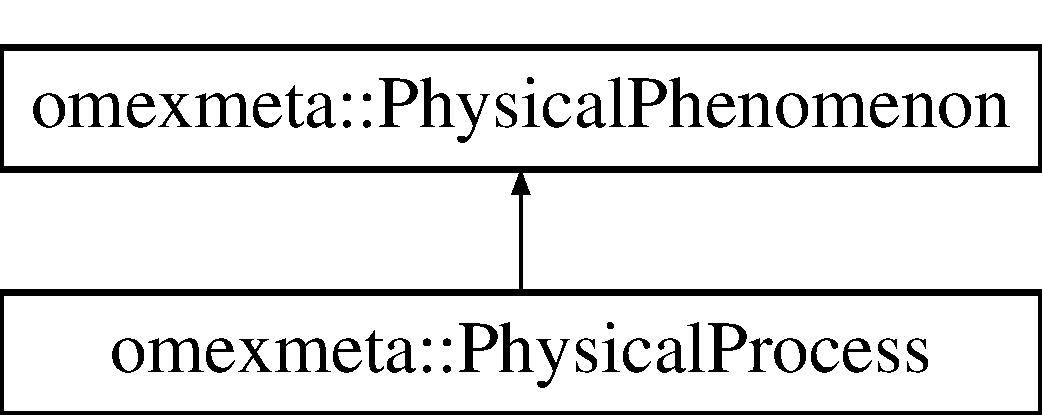
\includegraphics[height=2.000000cm]{classomexmeta_1_1PhysicalProcess}
\end{center}
\end{figure}
\subsection*{Public Member Functions}
\begin{DoxyCompactItemize}
\item 
\mbox{\Hypertarget{classomexmeta_1_1PhysicalProcess_a37f99033da4635ff1af2b9f19c1b84ce}\label{classomexmeta_1_1PhysicalProcess_a37f99033da4635ff1af2b9f19c1b84ce}} 
{\bfseries Physical\+Process} (librdf\+\_\+model $\ast$model, std\+::string model\+\_\+uri, std\+::string local\+\_\+uri, const \hyperlink{classomexmeta_1_1PhysicalProperty}{Physical\+Property} \&physical\+Property, Sources sources, Sinks sinks, Mediators mediators)
\item 
\mbox{\Hypertarget{classomexmeta_1_1PhysicalProcess_a8dfcffe80f264ad24e70de9d7b71c73b}\label{classomexmeta_1_1PhysicalProcess_a8dfcffe80f264ad24e70de9d7b71c73b}} 
void {\bfseries free} ()
\item 
\mbox{\Hypertarget{classomexmeta_1_1PhysicalProcess_a2b694395a318335e81c884ed76b5f4dd}\label{classomexmeta_1_1PhysicalProcess_a2b694395a318335e81c884ed76b5f4dd}} 
{\bfseries Physical\+Process} (librdf\+\_\+model $\ast$model)
\item 
\mbox{\Hypertarget{classomexmeta_1_1PhysicalProcess_a974e2717dbf4b690b95b07e9c026fd2a}\label{classomexmeta_1_1PhysicalProcess_a974e2717dbf4b690b95b07e9c026fd2a}} 
{\bfseries Physical\+Process} (librdf\+\_\+model $\ast$model, std\+::string model\+\_\+uri, std\+::string local\+\_\+uri)
\item 
\mbox{\Hypertarget{classomexmeta_1_1PhysicalProcess_ab5f3100febc21173775a2090bb57a0fb}\label{classomexmeta_1_1PhysicalProcess_ab5f3100febc21173775a2090bb57a0fb}} 
const Sources \& {\bfseries get\+Sources} () const
\item 
\mbox{\Hypertarget{classomexmeta_1_1PhysicalProcess_a069e7caa05f346f90f413f650f081535}\label{classomexmeta_1_1PhysicalProcess_a069e7caa05f346f90f413f650f081535}} 
const Sinks \& {\bfseries get\+Sinks} () const
\item 
\mbox{\Hypertarget{classomexmeta_1_1PhysicalProcess_a349b76ad1831d2510904510583f0d7f2}\label{classomexmeta_1_1PhysicalProcess_a349b76ad1831d2510904510583f0d7f2}} 
const Mediators \& {\bfseries get\+Mediators} () const
\item 
\mbox{\Hypertarget{classomexmeta_1_1PhysicalProcess_ab6f6af00fac2401f9a88e186fd1d897a}\label{classomexmeta_1_1PhysicalProcess_ab6f6af00fac2401f9a88e186fd1d897a}} 
\hyperlink{classomexmeta_1_1Triples}{Triples} {\bfseries to\+Triples} () override
\item 
\mbox{\Hypertarget{classomexmeta_1_1PhysicalProcess_ac875058d67408246aa28cf58dd77ccf6}\label{classomexmeta_1_1PhysicalProcess_ac875058d67408246aa28cf58dd77ccf6}} 
\hyperlink{classomexmeta_1_1PhysicalProcess}{Physical\+Process} \& {\bfseries set\+Physical\+Property} (std\+::string subject\+\_\+metaid, const std\+::string \&physical\+Property)
\item 
\mbox{\Hypertarget{classomexmeta_1_1PhysicalProcess_ac49bf4a1c21c6590a9d2af7ae93e13a7}\label{classomexmeta_1_1PhysicalProcess_ac49bf4a1c21c6590a9d2af7ae93e13a7}} 
\hyperlink{classomexmeta_1_1PhysicalProcess}{Physical\+Process} \& {\bfseries set\+Physical\+Property} (\hyperlink{classomexmeta_1_1PhysicalProperty}{Physical\+Property} physical\+Property)
\item 
\mbox{\Hypertarget{classomexmeta_1_1PhysicalProcess_ab83f58b7df77fdee131c22c71da22f39}\label{classomexmeta_1_1PhysicalProcess_ab83f58b7df77fdee131c22c71da22f39}} 
\hyperlink{classomexmeta_1_1PhysicalProcess}{Physical\+Process} \& {\bfseries add\+Source} (int multiplier, std\+::string physical\+\_\+entity\+\_\+reference)
\item 
\mbox{\Hypertarget{classomexmeta_1_1PhysicalProcess_a403ffc7d7d29702f2ff4e56084a1d714}\label{classomexmeta_1_1PhysicalProcess_a403ffc7d7d29702f2ff4e56084a1d714}} 
\hyperlink{classomexmeta_1_1PhysicalProcess}{Physical\+Process} \& {\bfseries add\+Sink} (int multiplier, std\+::string physical\+\_\+entity\+\_\+reference)
\item 
\mbox{\Hypertarget{classomexmeta_1_1PhysicalProcess_a2bdf8dde5ffa6b38d5042db49fd211d1}\label{classomexmeta_1_1PhysicalProcess_a2bdf8dde5ffa6b38d5042db49fd211d1}} 
\hyperlink{classomexmeta_1_1PhysicalProcess}{Physical\+Process} \& {\bfseries add\+Mediator} (std\+::string physical\+\_\+entity\+\_\+reference)
\item 
\mbox{\Hypertarget{classomexmeta_1_1PhysicalProcess_a56459d9f0087a3f92b0aca5d148b65f5}\label{classomexmeta_1_1PhysicalProcess_a56459d9f0087a3f92b0aca5d148b65f5}} 
int {\bfseries get\+Num\+Sources} ()
\item 
\mbox{\Hypertarget{classomexmeta_1_1PhysicalProcess_ac8b79af15d4d19042ee34abca25f679f}\label{classomexmeta_1_1PhysicalProcess_ac8b79af15d4d19042ee34abca25f679f}} 
int {\bfseries get\+Num\+Sinks} ()
\item 
\mbox{\Hypertarget{classomexmeta_1_1PhysicalProcess_a717a352ce3bb956201174002f904cd26}\label{classomexmeta_1_1PhysicalProcess_a717a352ce3bb956201174002f904cd26}} 
int {\bfseries get\+Num\+Mediators} ()
\item 
\mbox{\Hypertarget{classomexmeta_1_1PhysicalProcess_a65585bf5cd473d509f6f66c96757ff8d}\label{classomexmeta_1_1PhysicalProcess_a65585bf5cd473d509f6f66c96757ff8d}} 
bool {\bfseries operator==} (const \hyperlink{classomexmeta_1_1PhysicalProcess}{Physical\+Process} \&rhs) const
\item 
\mbox{\Hypertarget{classomexmeta_1_1PhysicalProcess_af8298394b713807ec51c2b5f60afd00e}\label{classomexmeta_1_1PhysicalProcess_af8298394b713807ec51c2b5f60afd00e}} 
bool {\bfseries operator!=} (const \hyperlink{classomexmeta_1_1PhysicalProcess}{Physical\+Process} \&rhs) const
\end{DoxyCompactItemize}
\subsection*{Additional Inherited Members}


The documentation for this class was generated from the following files\+:\begin{DoxyCompactItemize}
\item 
src/omexmeta/Physical\+Process.\+h\item 
src/omexmeta/Physical\+Process.\+cpp\end{DoxyCompactItemize}

\hypertarget{classomexmeta_1_1PhysicalProperty}{}\doxysection{omexmeta\+::Physical\+Property Class Reference}
\label{classomexmeta_1_1PhysicalProperty}\index{omexmeta::PhysicalProperty@{omexmeta::PhysicalProperty}}
\doxysubsection*{Public Member Functions}
\begin{DoxyCompactItemize}
\item 
\mbox{\Hypertarget{classomexmeta_1_1PhysicalProperty_ace1dfc8b0c7fc6bb23cd3d8c2126a49f}\label{classomexmeta_1_1PhysicalProperty_ace1dfc8b0c7fc6bb23cd3d8c2126a49f}} 
{\bfseries Physical\+Property} (\mbox{\hyperlink{classredland_1_1LibrdfModel}{Librdf\+Model}} \&model, \mbox{\hyperlink{classomexmeta_1_1UriHandler}{Uri\+Handler}} \&uri\+Handler)
\item 
\mbox{\Hypertarget{classomexmeta_1_1PhysicalProperty_a41cd211e575a4cf4144fa2157f52747d}\label{classomexmeta_1_1PhysicalProperty_a41cd211e575a4cf4144fa2157f52747d}} 
{\bfseries Physical\+Property} (const \mbox{\hyperlink{classomexmeta_1_1PhysicalProperty}{Physical\+Property}} \&physical\+Property)=default
\item 
\mbox{\Hypertarget{classomexmeta_1_1PhysicalProperty_a0c12f4fc60d445adf9a7086f76015474}\label{classomexmeta_1_1PhysicalProperty_a0c12f4fc60d445adf9a7086f76015474}} 
{\bfseries Physical\+Property} (\mbox{\hyperlink{classomexmeta_1_1PhysicalProperty}{Physical\+Property}} \&\&physical\+Property) noexcept=default
\item 
\mbox{\Hypertarget{classomexmeta_1_1PhysicalProperty_af0fc85f08d59093673270cf74773823e}\label{classomexmeta_1_1PhysicalProperty_af0fc85f08d59093673270cf74773823e}} 
\mbox{\hyperlink{classomexmeta_1_1PhysicalProperty}{Physical\+Property}} \& {\bfseries operator=} (const \mbox{\hyperlink{classomexmeta_1_1PhysicalProperty}{Physical\+Property}} \&physical\+Property)
\item 
\mbox{\Hypertarget{classomexmeta_1_1PhysicalProperty_a8800365ed17c49d1a8e7eb2225bae169}\label{classomexmeta_1_1PhysicalProperty_a8800365ed17c49d1a8e7eb2225bae169}} 
\mbox{\hyperlink{classomexmeta_1_1PhysicalProperty}{Physical\+Property}} \& {\bfseries operator=} (\mbox{\hyperlink{classomexmeta_1_1PhysicalProperty}{Physical\+Property}} \&\&physical\+Property) noexcept
\item 
\mbox{\Hypertarget{classomexmeta_1_1PhysicalProperty_a13a9ec404ea9c6d7ddea6c7398b67328}\label{classomexmeta_1_1PhysicalProperty_a13a9ec404ea9c6d7ddea6c7398b67328}} 
bool {\bfseries is\+Set} () const
\item 
\mbox{\Hypertarget{classomexmeta_1_1PhysicalProperty_a46f5436faa6f1c977088544bec31d125}\label{classomexmeta_1_1PhysicalProperty_a46f5436faa6f1c977088544bec31d125}} 
void {\bfseries set\+Is\+Set} (bool is\+Set)
\item 
\mbox{\Hypertarget{classomexmeta_1_1PhysicalProperty_a101d24ba21354367e13406d1f68c9248}\label{classomexmeta_1_1PhysicalProperty_a101d24ba21354367e13406d1f68c9248}} 
void {\bfseries set\+Property\+Metaid\+Base} (const std\+::string \&property\+Metaid\+Base)
\item 
\mbox{\Hypertarget{classomexmeta_1_1PhysicalProperty_aa9f55839baebd3594e859d4ad8d080a2}\label{classomexmeta_1_1PhysicalProperty_aa9f55839baebd3594e859d4ad8d080a2}} 
const std\+::string \& {\bfseries get\+Property\+Bearer\+Base} () const
\item 
\mbox{\Hypertarget{classomexmeta_1_1PhysicalProperty_a1b521c8ed4752a27b0e667c766b9e304}\label{classomexmeta_1_1PhysicalProperty_a1b521c8ed4752a27b0e667c766b9e304}} 
void {\bfseries set\+Property\+Bearer\+Base} (const std\+::string \&property\+Bearer\+Base)
\item 
\mbox{\Hypertarget{classomexmeta_1_1PhysicalProperty_a0f27071bfef5a9de4eb89fb21461ba76}\label{classomexmeta_1_1PhysicalProperty_a0f27071bfef5a9de4eb89fb21461ba76}} 
const std\+::string \& {\bfseries get\+Model\+Uri} () const
\item 
\mbox{\Hypertarget{classomexmeta_1_1PhysicalProperty_a9810bdd4b71d035e6187347b640ce83f}\label{classomexmeta_1_1PhysicalProperty_a9810bdd4b71d035e6187347b640ce83f}} 
const std\+::string \& {\bfseries get\+About} () const
\item 
\mbox{\Hypertarget{classomexmeta_1_1PhysicalProperty_a8065f6509c81feb045a13bcfe43c11b5}\label{classomexmeta_1_1PhysicalProperty_a8065f6509c81feb045a13bcfe43c11b5}} 
\mbox{\hyperlink{classomexmeta_1_1PhysicalProperty}{Physical\+Property}} \& {\bfseries about} (const std\+::string \&about, e\+Uri\+Type type=e\+Uri\+Type\+::\+NONE)
\item 
\mbox{\Hypertarget{classomexmeta_1_1PhysicalProperty_a182ba6fca7c913219ccd50e006cfbb61}\label{classomexmeta_1_1PhysicalProperty_a182ba6fca7c913219ccd50e006cfbb61}} 
const std\+::string \& {\bfseries get\+Is\+Version\+Of\+Value} () const
\item 
\mbox{\hyperlink{classomexmeta_1_1Triples}{Triples}} \mbox{\hyperlink{classomexmeta_1_1PhysicalProperty_af2e63778f1281f871a99e216bfcbaf88}{to\+Triples}} ()
\begin{DoxyCompactList}\small\item\em creates a \mbox{\hyperlink{classomexmeta_1_1Triples}{Triples}} object using the information in the \mbox{\hyperlink{classomexmeta_1_1PhysicalProperty}{Physical\+Property}} \end{DoxyCompactList}\item 
\mbox{\Hypertarget{classomexmeta_1_1PhysicalProperty_a57779b9711e41a3e70213190759b3d32}\label{classomexmeta_1_1PhysicalProperty_a57779b9711e41a3e70213190759b3d32}} 
\mbox{\hyperlink{classomexmeta_1_1PhysicalProperty}{Physical\+Property}} \& {\bfseries is\+Property\+Of} (const std\+::string \&is\+\_\+property\+\_\+of, e\+Uri\+Type type)
\item 
\mbox{\Hypertarget{classomexmeta_1_1PhysicalProperty_a30ca01ca75b8ccb6293f515439b00e06}\label{classomexmeta_1_1PhysicalProperty_a30ca01ca75b8ccb6293f515439b00e06}} 
\mbox{\hyperlink{classomexmeta_1_1PhysicalProperty}{Physical\+Property}} \& {\bfseries is\+Version\+Of} (const std\+::string \&resource)
\item 
\mbox{\Hypertarget{classomexmeta_1_1PhysicalProperty_ab498df5bb21e010614ae43c0c8e70bb7}\label{classomexmeta_1_1PhysicalProperty_ab498df5bb21e010614ae43c0c8e70bb7}} 
const std\+::string \& {\bfseries get\+Local\+Uri} () const
\item 
\mbox{\Hypertarget{classomexmeta_1_1PhysicalProperty_a6981edb407fb11b81eebccbc8f7aa94a}\label{classomexmeta_1_1PhysicalProperty_a6981edb407fb11b81eebccbc8f7aa94a}} 
const std\+::string \& {\bfseries get\+Is\+Property\+Of\+Value} () const
\item 
\mbox{\Hypertarget{classomexmeta_1_1PhysicalProperty_acd67e442b842ba57daf0653467b8a682}\label{classomexmeta_1_1PhysicalProperty_acd67e442b842ba57daf0653467b8a682}} 
const std\+::string \& {\bfseries get\+Property\+Metaid\+Base} () const
\item 
\mbox{\Hypertarget{classomexmeta_1_1PhysicalProperty_af3b3379a751ebb15f7a5ea0cae8cb4d6}\label{classomexmeta_1_1PhysicalProperty_af3b3379a751ebb15f7a5ea0cae8cb4d6}} 
bool {\bfseries operator==} (const \mbox{\hyperlink{classomexmeta_1_1PhysicalProperty}{Physical\+Property}} \&rhs) const
\item 
\mbox{\Hypertarget{classomexmeta_1_1PhysicalProperty_a1a85ba2c50f5b79e49e8a01b96756f0a}\label{classomexmeta_1_1PhysicalProperty_a1a85ba2c50f5b79e49e8a01b96756f0a}} 
bool {\bfseries operator!=} (const \mbox{\hyperlink{classomexmeta_1_1PhysicalProperty}{Physical\+Property}} \&rhs) const
\end{DoxyCompactItemize}


\doxysubsection{Member Function Documentation}
\mbox{\Hypertarget{classomexmeta_1_1PhysicalProperty_af2e63778f1281f871a99e216bfcbaf88}\label{classomexmeta_1_1PhysicalProperty_af2e63778f1281f871a99e216bfcbaf88}} 
\index{omexmeta::PhysicalProperty@{omexmeta::PhysicalProperty}!toTriples@{toTriples}}
\index{toTriples@{toTriples}!omexmeta::PhysicalProperty@{omexmeta::PhysicalProperty}}
\doxysubsubsection{\texorpdfstring{toTriples()}{toTriples()}}
{\footnotesize\ttfamily \mbox{\hyperlink{classomexmeta_1_1Triples}{Triples}} omexmeta\+::\+Physical\+Property\+::to\+Triples (\begin{DoxyParamCaption}{ }\end{DoxyParamCaption})}



creates a \mbox{\hyperlink{classomexmeta_1_1Triples}{Triples}} object using the information in the \mbox{\hyperlink{classomexmeta_1_1PhysicalProperty}{Physical\+Property}} 

\begin{DoxyReturn}{Returns}
a \mbox{\hyperlink{classomexmeta_1_1Triples}{Triples}} object containing the set of \mbox{\hyperlink{classomexmeta_1_1Triple}{Triple}} object used to represent this \mbox{\hyperlink{classomexmeta_1_1PhysicalProperty}{Physical\+Property}} 
\end{DoxyReturn}


The documentation for this class was generated from the following files\+:\begin{DoxyCompactItemize}
\item 
src/omexmeta/include/omexmeta/Physical\+Property.\+h\item 
src/omexmeta/Physical\+Property.\+cpp\end{DoxyCompactItemize}

\hypertarget{classomexmeta_1_1Predicate}{}\doxysection{omexmeta\+::Predicate Class Reference}
\label{classomexmeta_1_1Predicate}\index{omexmeta::Predicate@{omexmeta::Predicate}}


{\ttfamily \#include $<$Predicate.\+h$>$}

Inheritance diagram for omexmeta\+::Predicate\+:\begin{figure}[H]
\begin{center}
\leavevmode
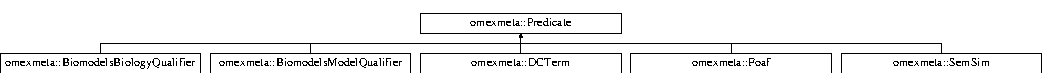
\includegraphics[height=0.978166cm]{classomexmeta_1_1Predicate}
\end{center}
\end{figure}
\doxysubsection*{Public Member Functions}
\begin{DoxyCompactItemize}
\item 
\mbox{\hyperlink{classomexmeta_1_1Predicate_ad5a91eb29204202d2f18816d09677622}{Predicate}} (const std\+::string \&\mbox{\hyperlink{classomexmeta_1_1Predicate_afc79b0cc43eb11e4bc2fe0b305e551bc}{namespace\+\_\+}}, std\+::string term, std\+::string prefix)
\begin{DoxyCompactList}\small\item\em construct a \mbox{\hyperlink{classomexmeta_1_1Predicate}{Predicate}} from a namespace, term and prefix portion of a predicate \end{DoxyCompactList}\item 
\mbox{\Hypertarget{classomexmeta_1_1Predicate_a5db1e6150f8cfd7605e82996e2aebb50}\label{classomexmeta_1_1Predicate_a5db1e6150f8cfd7605e82996e2aebb50}} 
bool {\bfseries operator==} (const \mbox{\hyperlink{classomexmeta_1_1Predicate}{Predicate}} \&rhs) const
\item 
\mbox{\Hypertarget{classomexmeta_1_1Predicate_a7bf4b8769eb9801eb26cc976723b56f2}\label{classomexmeta_1_1Predicate_a7bf4b8769eb9801eb26cc976723b56f2}} 
bool {\bfseries operator!=} (const \mbox{\hyperlink{classomexmeta_1_1Predicate}{Predicate}} \&rhs) const
\item 
std\+::string \mbox{\hyperlink{classomexmeta_1_1Predicate_a9d51ebf565f39fb4d6d4f58c1b030edf}{str}} ()
\begin{DoxyCompactList}\small\item\em get the predicate as a full string \end{DoxyCompactList}\item 
\mbox{\hyperlink{structraptor__term}{librdf\+\_\+node}} $\ast$ \mbox{\hyperlink{classomexmeta_1_1Predicate_a6edbc1f17d4a5cbf8ad0c1b70b683b4a}{get}} () const
\begin{DoxyCompactList}\small\item\em getter for the node contained by the \mbox{\hyperlink{classomexmeta_1_1Predicate}{Predicate}} object \end{DoxyCompactList}\item 
const std\+::vector$<$ std\+::string $>$ \& \mbox{\hyperlink{classomexmeta_1_1Predicate_aee19b8fc8b21f8e5ffd5b64691e1e530}{get\+Valid\+Terms}} () const
\begin{DoxyCompactList}\small\item\em stores the valid terms that are allowed in a particular predicate subclass \end{DoxyCompactList}\item 
const std\+::string \& \mbox{\hyperlink{classomexmeta_1_1Predicate_add4ab1cd86f83de3512279bbfdad947c}{get\+Namespace}} () const
\begin{DoxyCompactList}\small\item\em getter for the namespace portion of the \mbox{\hyperlink{classomexmeta_1_1Predicate}{Predicate}} \end{DoxyCompactList}\item 
const std\+::string \& \mbox{\hyperlink{classomexmeta_1_1Predicate_a54a15176bd697d37d00573bf86954630}{get\+Term}} () const
\begin{DoxyCompactList}\small\item\em getter for term portion of the \mbox{\hyperlink{classomexmeta_1_1Predicate}{Predicate}} \end{DoxyCompactList}\item 
const std\+::string \& \mbox{\hyperlink{classomexmeta_1_1Predicate_a0147e977f71604db05763815ae6b553f}{get\+Prefix}} () const
\begin{DoxyCompactList}\small\item\em getter for the prefix portion of the \mbox{\hyperlink{classomexmeta_1_1Predicate}{Predicate}} \end{DoxyCompactList}\item 
const std\+::string \& \mbox{\hyperlink{classomexmeta_1_1Predicate_a27fa7d62ad9a5182f3dd642bc61c8d9f}{get\+Uri}} () const
\begin{DoxyCompactList}\small\item\em getter for uri \end{DoxyCompactList}\item 
void \mbox{\hyperlink{classomexmeta_1_1Predicate_a718a37ff90ac0f2d7cc129e8351a2c7b}{free\+Node}} ()
\begin{DoxyCompactList}\small\item\em release resources associated with this \mbox{\hyperlink{classomexmeta_1_1Predicate}{Predicate}}. \end{DoxyCompactList}\item 
void \mbox{\hyperlink{classomexmeta_1_1Predicate_a0bf6030510247a6999d81cada92c1e51}{set\+Node}} (\mbox{\hyperlink{structraptor__term}{librdf\+\_\+node}} $\ast$node)
\begin{DoxyCompactList}\small\item\em replace the current librdf\+\_\+node assicated with this \mbox{\hyperlink{classomexmeta_1_1Predicate}{Predicate}} with node \end{DoxyCompactList}\item 
\mbox{\Hypertarget{classomexmeta_1_1Predicate_ae2adc312e293aabfdbbffbb44018665b}\label{classomexmeta_1_1Predicate_ae2adc312e293aabfdbbffbb44018665b}} 
\mbox{\hyperlink{classredland_1_1LibrdfNode}{Librdf\+Node}} {\bfseries get\+Node} ()
\end{DoxyCompactItemize}
\doxysubsection*{Static Public Member Functions}
\begin{DoxyCompactItemize}
\item 
static std\+::unordered\+\_\+map$<$ std\+::string, std\+::string $>$ \mbox{\hyperlink{classomexmeta_1_1Predicate_a1291e3cd9727871f568e864e0f5af3f0}{namespace\+Map}} ()
\begin{DoxyCompactList}\small\item\em get a map namespaces and prefixes \end{DoxyCompactList}\item 
static void \mbox{\hyperlink{classomexmeta_1_1Predicate_a1e7e59b8a48c9f89eeec73f3bbaea19c}{verify}} (std\+::vector$<$ std\+::string $>$ valid\+\_\+terms, const std\+::string \&term)
\begin{DoxyCompactList}\small\item\em Static method for checking validity of term against valid\+\_\+terms. \end{DoxyCompactList}\item 
static bool \mbox{\hyperlink{classomexmeta_1_1Predicate_a8381c8b0c7bbaa27de29608cbff08bf5}{namespace\+Known}} (const std\+::string \&ns)
\begin{DoxyCompactList}\small\item\em check if we have \char`\"{}know\char`\"{} a namespace. Known namespaces are returned by \mbox{\hyperlink{classomexmeta_1_1Predicate_a1291e3cd9727871f568e864e0f5af3f0}{Predicate\+::namespace\+Map()}}. \end{DoxyCompactList}\item 
\mbox{\Hypertarget{classomexmeta_1_1Predicate_a4cda551beb4e1354ac56d692f0eb78cd}\label{classomexmeta_1_1Predicate_a4cda551beb4e1354ac56d692f0eb78cd}} 
static void \mbox{\hyperlink{classomexmeta_1_1Predicate_a4cda551beb4e1354ac56d692f0eb78cd}{add\+Seen\+Namespace\+To\+Serializer}} (librdf\+\_\+world $\ast$world, librdf\+\_\+serializer $\ast$serializer, \mbox{\hyperlink{structraptor__term}{librdf\+\_\+node}} $\ast$predicate)
\begin{DoxyCompactList}\small\item\em utility for checking whether the uri in @parameter predicate has a namespace that we already know. If found, the namespace is added to @parameter serializer \end{DoxyCompactList}\end{DoxyCompactItemize}
\doxysubsection*{Protected Member Functions}
\begin{DoxyCompactItemize}
\item 
\mbox{\Hypertarget{classomexmeta_1_1Predicate_a157c4e95f9869d4f22cd07332ff7621a}\label{classomexmeta_1_1Predicate_a157c4e95f9869d4f22cd07332ff7621a}} 
{\bfseries Predicate} (\mbox{\hyperlink{structraptor__term}{librdf\+\_\+node}} $\ast$node)
\end{DoxyCompactItemize}
\doxysubsection*{Protected Attributes}
\begin{DoxyCompactItemize}
\item 
\mbox{\Hypertarget{classomexmeta_1_1Predicate_afc79b0cc43eb11e4bc2fe0b305e551bc}\label{classomexmeta_1_1Predicate_afc79b0cc43eb11e4bc2fe0b305e551bc}} 
std\+::string \mbox{\hyperlink{classomexmeta_1_1Predicate_afc79b0cc43eb11e4bc2fe0b305e551bc}{namespace\+\_\+}}
\begin{DoxyCompactList}\small\item\em make a shared pointer from this \mbox{\hyperlink{classomexmeta_1_1Predicate}{Predicate}} \end{DoxyCompactList}\item 
\mbox{\Hypertarget{classomexmeta_1_1Predicate_ab626a5fd9fa8f302767d4ca544a9eff2}\label{classomexmeta_1_1Predicate_ab626a5fd9fa8f302767d4ca544a9eff2}} 
std\+::string {\bfseries term\+\_\+}
\item 
\mbox{\Hypertarget{classomexmeta_1_1Predicate_a5dfbbc85f7bdc5a3e4da72913f6ce306}\label{classomexmeta_1_1Predicate_a5dfbbc85f7bdc5a3e4da72913f6ce306}} 
std\+::string {\bfseries prefix\+\_\+}
\item 
\mbox{\Hypertarget{classomexmeta_1_1Predicate_a4fe359b93a9dea9b60f7bc28c1aa913b}\label{classomexmeta_1_1Predicate_a4fe359b93a9dea9b60f7bc28c1aa913b}} 
std\+::string {\bfseries uri\+\_\+}
\item 
\mbox{\Hypertarget{classomexmeta_1_1Predicate_a14ae7768fbd3aaf444bcde8650910c0b}\label{classomexmeta_1_1Predicate_a14ae7768fbd3aaf444bcde8650910c0b}} 
std\+::vector$<$ std\+::string $>$ {\bfseries valid\+\_\+terms\+\_\+} \{\char`\"{}All\char`\"{}\}
\item 
\mbox{\Hypertarget{classomexmeta_1_1Predicate_a1c062fe0337919ecbffba1f567b77048}\label{classomexmeta_1_1Predicate_a1c062fe0337919ecbffba1f567b77048}} 
\mbox{\hyperlink{classredland_1_1LibrdfNode}{Librdf\+Node}} {\bfseries node\+\_\+}
\end{DoxyCompactItemize}


\doxysubsection{Detailed Description}
The predicate class creates and stores a URI node. 

\doxysubsection{Constructor \& Destructor Documentation}
\mbox{\Hypertarget{classomexmeta_1_1Predicate_ad5a91eb29204202d2f18816d09677622}\label{classomexmeta_1_1Predicate_ad5a91eb29204202d2f18816d09677622}} 
\index{omexmeta::Predicate@{omexmeta::Predicate}!Predicate@{Predicate}}
\index{Predicate@{Predicate}!omexmeta::Predicate@{omexmeta::Predicate}}
\doxysubsubsection{\texorpdfstring{Predicate()}{Predicate()}}
{\footnotesize\ttfamily omexmeta\+::\+Predicate\+::\+Predicate (\begin{DoxyParamCaption}\item[{const std\+::string \&}]{namespace\+\_\+,  }\item[{std\+::string}]{term,  }\item[{std\+::string}]{prefix }\end{DoxyParamCaption})}



construct a \mbox{\hyperlink{classomexmeta_1_1Predicate}{Predicate}} from a namespace, term and prefix portion of a predicate 


\begin{DoxyParams}{Parameters}
{\em namespace\+\_\+} & the namespace portion of a predicate. i.\+e. \href{http://biomodels.net/biology-qualifiers/}{\texttt{ http\+://biomodels.\+net/biology-\/qualifiers/}} \\
\hline
{\em term} & the last portion of the predicate, i.\+e. is \\
\hline
{\em prefix} & the prefix that can be used instead of the full namespace, i.\+e. bqbiol\\
\hline
\end{DoxyParams}
\href{http://biomodels.net/biology-qualifiers/is}{\texttt{ http\+://biomodels.\+net/biology-\/qualifiers/is}} -\/-\/-\/-\/-\/-\/-\/-\/-\/-\/-\/-\/-\/-\/-\/-\/-\/-\/-\/-\/-\/-\/-\/-\/-\/-\/-\/-\/-\/-\/-\/-\/-\/-\/-\/-\/---$\vert$-- $\vert$ $\vert$ namespace term

is equivalent to

bqbiol\+:is -\/-\/-\/---$\vert$-- $\vert$ $\vert$ prefix term 

\doxysubsection{Member Function Documentation}
\mbox{\Hypertarget{classomexmeta_1_1Predicate_a718a37ff90ac0f2d7cc129e8351a2c7b}\label{classomexmeta_1_1Predicate_a718a37ff90ac0f2d7cc129e8351a2c7b}} 
\index{omexmeta::Predicate@{omexmeta::Predicate}!freeNode@{freeNode}}
\index{freeNode@{freeNode}!omexmeta::Predicate@{omexmeta::Predicate}}
\doxysubsubsection{\texorpdfstring{freeNode()}{freeNode()}}
{\footnotesize\ttfamily void omexmeta\+::\+Predicate\+::free\+Node (\begin{DoxyParamCaption}{ }\end{DoxyParamCaption})}



release resources associated with this \mbox{\hyperlink{classomexmeta_1_1Predicate}{Predicate}}. 

\mbox{\hyperlink{classomexmeta_1_1Predicate}{Predicate}} objects contain a librdf\+\_\+node pointer which needs to be freed by the caller. If a \mbox{\hyperlink{classomexmeta_1_1Predicate}{Predicate}} is passed to a \mbox{\hyperlink{classomexmeta_1_1Triple}{Triple}} object (which most of the time is it), responsibility for deleting the contained librdf\+\_\+node is transferred to the \mbox{\hyperlink{classomexmeta_1_1Triple}{Triple}} object, which automatically clears up resources. If not, then it is the callers responsibility to call this method when they are done with \mbox{\hyperlink{classomexmeta_1_1Predicate}{Predicate}} instances. \mbox{\Hypertarget{classomexmeta_1_1Predicate_a6edbc1f17d4a5cbf8ad0c1b70b683b4a}\label{classomexmeta_1_1Predicate_a6edbc1f17d4a5cbf8ad0c1b70b683b4a}} 
\index{omexmeta::Predicate@{omexmeta::Predicate}!get@{get}}
\index{get@{get}!omexmeta::Predicate@{omexmeta::Predicate}}
\doxysubsubsection{\texorpdfstring{get()}{get()}}
{\footnotesize\ttfamily \mbox{\hyperlink{structraptor__term}{librdf\+\_\+node}} $\ast$ omexmeta\+::\+Predicate\+::get (\begin{DoxyParamCaption}{ }\end{DoxyParamCaption}) const}



getter for the node contained by the \mbox{\hyperlink{classomexmeta_1_1Predicate}{Predicate}} object 

\begin{DoxyReturn}{Returns}
the librdf\+\_\+node$\ast$ pointer for the redland libraries under the hood 
\end{DoxyReturn}
\mbox{\Hypertarget{classomexmeta_1_1Predicate_add4ab1cd86f83de3512279bbfdad947c}\label{classomexmeta_1_1Predicate_add4ab1cd86f83de3512279bbfdad947c}} 
\index{omexmeta::Predicate@{omexmeta::Predicate}!getNamespace@{getNamespace}}
\index{getNamespace@{getNamespace}!omexmeta::Predicate@{omexmeta::Predicate}}
\doxysubsubsection{\texorpdfstring{getNamespace()}{getNamespace()}}
{\footnotesize\ttfamily const std\+::string \& omexmeta\+::\+Predicate\+::get\+Namespace (\begin{DoxyParamCaption}{ }\end{DoxyParamCaption}) const}



getter for the namespace portion of the \mbox{\hyperlink{classomexmeta_1_1Predicate}{Predicate}} 

\begin{DoxyReturn}{Returns}
the string representing the namespace of the current \mbox{\hyperlink{classomexmeta_1_1Predicate}{Predicate}} 
\end{DoxyReturn}
\mbox{\Hypertarget{classomexmeta_1_1Predicate_a0147e977f71604db05763815ae6b553f}\label{classomexmeta_1_1Predicate_a0147e977f71604db05763815ae6b553f}} 
\index{omexmeta::Predicate@{omexmeta::Predicate}!getPrefix@{getPrefix}}
\index{getPrefix@{getPrefix}!omexmeta::Predicate@{omexmeta::Predicate}}
\doxysubsubsection{\texorpdfstring{getPrefix()}{getPrefix()}}
{\footnotesize\ttfamily const std\+::string \& omexmeta\+::\+Predicate\+::get\+Prefix (\begin{DoxyParamCaption}{ }\end{DoxyParamCaption}) const}



getter for the prefix portion of the \mbox{\hyperlink{classomexmeta_1_1Predicate}{Predicate}} 

\begin{DoxyReturn}{Returns}
the string representing the prefix portion of the \mbox{\hyperlink{classomexmeta_1_1Predicate}{Predicate}} 
\end{DoxyReturn}
\mbox{\Hypertarget{classomexmeta_1_1Predicate_a54a15176bd697d37d00573bf86954630}\label{classomexmeta_1_1Predicate_a54a15176bd697d37d00573bf86954630}} 
\index{omexmeta::Predicate@{omexmeta::Predicate}!getTerm@{getTerm}}
\index{getTerm@{getTerm}!omexmeta::Predicate@{omexmeta::Predicate}}
\doxysubsubsection{\texorpdfstring{getTerm()}{getTerm()}}
{\footnotesize\ttfamily const std\+::string \& omexmeta\+::\+Predicate\+::get\+Term (\begin{DoxyParamCaption}{ }\end{DoxyParamCaption}) const}



getter for term portion of the \mbox{\hyperlink{classomexmeta_1_1Predicate}{Predicate}} 

\begin{DoxyReturn}{Returns}
the string representing the term portion of the \mbox{\hyperlink{classomexmeta_1_1Predicate}{Predicate}} 
\end{DoxyReturn}
\mbox{\Hypertarget{classomexmeta_1_1Predicate_a27fa7d62ad9a5182f3dd642bc61c8d9f}\label{classomexmeta_1_1Predicate_a27fa7d62ad9a5182f3dd642bc61c8d9f}} 
\index{omexmeta::Predicate@{omexmeta::Predicate}!getUri@{getUri}}
\index{getUri@{getUri}!omexmeta::Predicate@{omexmeta::Predicate}}
\doxysubsubsection{\texorpdfstring{getUri()}{getUri()}}
{\footnotesize\ttfamily const std\+::string \& omexmeta\+::\+Predicate\+::get\+Uri (\begin{DoxyParamCaption}{ }\end{DoxyParamCaption}) const}



getter for uri 

For developers. Consider removing since \mbox{\hyperlink{classomexmeta_1_1Predicate_a9d51ebf565f39fb4d6d4f58c1b030edf}{str()}} method does the same thing \mbox{\Hypertarget{classomexmeta_1_1Predicate_aee19b8fc8b21f8e5ffd5b64691e1e530}\label{classomexmeta_1_1Predicate_aee19b8fc8b21f8e5ffd5b64691e1e530}} 
\index{omexmeta::Predicate@{omexmeta::Predicate}!getValidTerms@{getValidTerms}}
\index{getValidTerms@{getValidTerms}!omexmeta::Predicate@{omexmeta::Predicate}}
\doxysubsubsection{\texorpdfstring{getValidTerms()}{getValidTerms()}}
{\footnotesize\ttfamily const std\+::vector$<$ std\+::string $>$ \& omexmeta\+::\+Predicate\+::get\+Valid\+Terms (\begin{DoxyParamCaption}{ }\end{DoxyParamCaption}) const}



stores the valid terms that are allowed in a particular predicate subclass 

\begin{DoxyReturn}{Returns}
a vector of strings
\end{DoxyReturn}
Subclasses override this method so they return a complete list of valid terms for their own class \mbox{\Hypertarget{classomexmeta_1_1Predicate_a8381c8b0c7bbaa27de29608cbff08bf5}\label{classomexmeta_1_1Predicate_a8381c8b0c7bbaa27de29608cbff08bf5}} 
\index{omexmeta::Predicate@{omexmeta::Predicate}!namespaceKnown@{namespaceKnown}}
\index{namespaceKnown@{namespaceKnown}!omexmeta::Predicate@{omexmeta::Predicate}}
\doxysubsubsection{\texorpdfstring{namespaceKnown()}{namespaceKnown()}}
{\footnotesize\ttfamily bool omexmeta\+::\+Predicate\+::namespace\+Known (\begin{DoxyParamCaption}\item[{const std\+::string \&}]{ns }\end{DoxyParamCaption})\hspace{0.3cm}{\ttfamily [static]}}



check if we have \char`\"{}know\char`\"{} a namespace. Known namespaces are returned by \mbox{\hyperlink{classomexmeta_1_1Predicate_a1291e3cd9727871f568e864e0f5af3f0}{Predicate\+::namespace\+Map()}}. 


\begin{DoxyParams}{Parameters}
{\em ns} & the namespace to check \\
\hline
\end{DoxyParams}
\begin{DoxyReturn}{Returns}
True if we have seen the namespace ns before 
\end{DoxyReturn}
\mbox{\Hypertarget{classomexmeta_1_1Predicate_a1291e3cd9727871f568e864e0f5af3f0}\label{classomexmeta_1_1Predicate_a1291e3cd9727871f568e864e0f5af3f0}} 
\index{omexmeta::Predicate@{omexmeta::Predicate}!namespaceMap@{namespaceMap}}
\index{namespaceMap@{namespaceMap}!omexmeta::Predicate@{omexmeta::Predicate}}
\doxysubsubsection{\texorpdfstring{namespaceMap()}{namespaceMap()}}
{\footnotesize\ttfamily std\+::unordered\+\_\+map$<$ std\+::string, std\+::string $>$ omexmeta\+::\+Predicate\+::namespace\+Map (\begin{DoxyParamCaption}{ }\end{DoxyParamCaption})\hspace{0.3cm}{\ttfamily [static]}}



get a map namespaces and prefixes 

\begin{DoxyReturn}{Returns}
a unordered\+\_\+map with namespaces as keys and prefixes as values 
\end{DoxyReturn}
\mbox{\Hypertarget{classomexmeta_1_1Predicate_a0bf6030510247a6999d81cada92c1e51}\label{classomexmeta_1_1Predicate_a0bf6030510247a6999d81cada92c1e51}} 
\index{omexmeta::Predicate@{omexmeta::Predicate}!setNode@{setNode}}
\index{setNode@{setNode}!omexmeta::Predicate@{omexmeta::Predicate}}
\doxysubsubsection{\texorpdfstring{setNode()}{setNode()}}
{\footnotesize\ttfamily void omexmeta\+::\+Predicate\+::set\+Node (\begin{DoxyParamCaption}\item[{\mbox{\hyperlink{structraptor__term}{librdf\+\_\+node}} $\ast$}]{node }\end{DoxyParamCaption})}



replace the current librdf\+\_\+node assicated with this \mbox{\hyperlink{classomexmeta_1_1Predicate}{Predicate}} with node 


\begin{DoxyParams}{Parameters}
{\em node} & the new librdf\+\_\+node pointer to use in the \mbox{\hyperlink{classomexmeta_1_1Predicate}{Predicate}} \\
\hline
\end{DoxyParams}
\mbox{\Hypertarget{classomexmeta_1_1Predicate_a9d51ebf565f39fb4d6d4f58c1b030edf}\label{classomexmeta_1_1Predicate_a9d51ebf565f39fb4d6d4f58c1b030edf}} 
\index{omexmeta::Predicate@{omexmeta::Predicate}!str@{str}}
\index{str@{str}!omexmeta::Predicate@{omexmeta::Predicate}}
\doxysubsubsection{\texorpdfstring{str()}{str()}}
{\footnotesize\ttfamily std\+::string omexmeta\+::\+Predicate\+::str (\begin{DoxyParamCaption}{ }\end{DoxyParamCaption})}



get the predicate as a full string 

\begin{DoxyReturn}{Returns}
a string representing the predicate 
\end{DoxyReturn}
\mbox{\Hypertarget{classomexmeta_1_1Predicate_a1e7e59b8a48c9f89eeec73f3bbaea19c}\label{classomexmeta_1_1Predicate_a1e7e59b8a48c9f89eeec73f3bbaea19c}} 
\index{omexmeta::Predicate@{omexmeta::Predicate}!verify@{verify}}
\index{verify@{verify}!omexmeta::Predicate@{omexmeta::Predicate}}
\doxysubsubsection{\texorpdfstring{verify()}{verify()}}
{\footnotesize\ttfamily void omexmeta\+::\+Predicate\+::verify (\begin{DoxyParamCaption}\item[{std\+::vector$<$ std\+::string $>$}]{valid\+\_\+terms,  }\item[{const std\+::string \&}]{term }\end{DoxyParamCaption})\hspace{0.3cm}{\ttfamily [static]}}



Static method for checking validity of term against valid\+\_\+terms. 


\begin{DoxyParams}{Parameters}
{\em term} & the term to validate \\
\hline
{\em valid\+\_\+terms} & the set of terms to validate term against\\
\hline
\end{DoxyParams}
Throws an error when term is not in valid\+\_\+terms. Used by subclasses to verify user input. 

The documentation for this class was generated from the following files\+:\begin{DoxyCompactItemize}
\item 
src/omexmeta/include/omexmeta/Predicate.\+h\item 
src/omexmeta/Predicate.\+cpp\end{DoxyCompactItemize}

\hypertarget{structdbg_1_1pretty__print__tuple}{}\section{dbg\+:\+:pretty\+\_\+print\+\_\+tuple$<$ Idx $>$ Struct Template Reference}
\label{structdbg_1_1pretty__print__tuple}\index{dbg\+::pretty\+\_\+print\+\_\+tuple$<$ Idx $>$@{dbg\+::pretty\+\_\+print\+\_\+tuple$<$ Idx $>$}}
\subsection*{Static Public Member Functions}
\begin{DoxyCompactItemize}
\item 
\mbox{\Hypertarget{structdbg_1_1pretty__print__tuple_a17c2bca6c330e88da2082efa4c3a9be5}\label{structdbg_1_1pretty__print__tuple_a17c2bca6c330e88da2082efa4c3a9be5}} 
{\footnotesize template$<$typename... Ts$>$ }\\static void {\bfseries print} (std\+::ostream \&stream, const std\+::tuple$<$ Ts... $>$ \&tuple)
\end{DoxyCompactItemize}


The documentation for this struct was generated from the following file\+:\begin{DoxyCompactItemize}
\item 
src/omexmeta/dbg.\+h\end{DoxyCompactItemize}

\hypertarget{structdbg_1_1pretty__print__tuple_3_010_01_4}{}\doxysection{dbg\+::pretty\+\_\+print\+\_\+tuple$<$ 0 $>$ Struct Reference}
\label{structdbg_1_1pretty__print__tuple_3_010_01_4}\index{dbg::pretty\_print\_tuple$<$ 0 $>$@{dbg::pretty\_print\_tuple$<$ 0 $>$}}
\doxysubsection*{Static Public Member Functions}
\begin{DoxyCompactItemize}
\item 
\mbox{\Hypertarget{structdbg_1_1pretty__print__tuple_3_010_01_4_a9961147d35a3bcc6b89af9610c68ad39}\label{structdbg_1_1pretty__print__tuple_3_010_01_4_a9961147d35a3bcc6b89af9610c68ad39}} 
{\footnotesize template$<$typename... Ts$>$ }\\static void {\bfseries print} (std\+::ostream \&stream, const std\+::tuple$<$ Ts... $>$ \&tuple)
\end{DoxyCompactItemize}


The documentation for this struct was generated from the following file\+:\begin{DoxyCompactItemize}
\item 
src/omexmeta/include/omexmeta/dbg.\+h\end{DoxyCompactItemize}

\hypertarget{structdbg_1_1print__formatted}{}\section{dbg\+:\+:print\+\_\+formatted$<$ T $>$ Struct Template Reference}
\label{structdbg_1_1print__formatted}\index{dbg\+::print\+\_\+formatted$<$ T $>$@{dbg\+::print\+\_\+formatted$<$ T $>$}}
\subsection*{Public Member Functions}
\begin{DoxyCompactItemize}
\item 
\mbox{\Hypertarget{structdbg_1_1print__formatted_a77fef2b6aa871171bfefe58bab8a03fe}\label{structdbg_1_1print__formatted_a77fef2b6aa871171bfefe58bab8a03fe}} 
{\bfseries print\+\_\+formatted} (T value, int numeric\+\_\+base)
\item 
\mbox{\Hypertarget{structdbg_1_1print__formatted_ab6a7c4280acb807f5c5ab812f80a8aca}\label{structdbg_1_1print__formatted_ab6a7c4280acb807f5c5ab812f80a8aca}} 
{\bfseries operator T} () const
\item 
\mbox{\Hypertarget{structdbg_1_1print__formatted_ab490d37d984d053177b6af3f94d0136e}\label{structdbg_1_1print__formatted_ab490d37d984d053177b6af3f94d0136e}} 
const char $\ast$ {\bfseries prefix} () const
\end{DoxyCompactItemize}
\subsection*{Public Attributes}
\begin{DoxyCompactItemize}
\item 
\mbox{\Hypertarget{structdbg_1_1print__formatted_a080056e4f7af0c86ed46bc2ecb9c6f1e}\label{structdbg_1_1print__formatted_a080056e4f7af0c86ed46bc2ecb9c6f1e}} 
T {\bfseries inner}
\item 
\mbox{\Hypertarget{structdbg_1_1print__formatted_af57ecb89743fca9b4cb1d0afd3c9d9f4}\label{structdbg_1_1print__formatted_af57ecb89743fca9b4cb1d0afd3c9d9f4}} 
int {\bfseries base}
\end{DoxyCompactItemize}


The documentation for this struct was generated from the following file\+:\begin{DoxyCompactItemize}
\item 
src/omexmeta/dbg.\+h\end{DoxyCompactItemize}

\hypertarget{structdbg_1_1print__type}{}\section{dbg\+:\+:print\+\_\+type$<$ T $>$ Struct Template Reference}
\label{structdbg_1_1print__type}\index{dbg\+::print\+\_\+type$<$ T $>$@{dbg\+::print\+\_\+type$<$ T $>$}}


The documentation for this struct was generated from the following file\+:\begin{DoxyCompactItemize}
\item 
src/omexmeta/dbg.\+h\end{DoxyCompactItemize}

\hypertarget{classomexmeta_1_1Query}{}\section{omexmeta\+:\+:Query Class Reference}
\label{classomexmeta_1_1Query}\index{omexmeta\+::\+Query@{omexmeta\+::\+Query}}
\subsection*{\+: variable name}
\label{_amgrp7ca1d8b10bb02d408ac42bd6ecaaf12b}%
librdf\+\_\+query\+\_\+results\+\_\+get\+\_\+binding\+\_\+value\+\_\+by\+\_\+name\+: \+: \#librdf\+\_\+query\+\_\+results query results

Get one binding value for a given name in the current result.

Return value\+: a new \#librdf\+\_\+node binding value or N\+U\+LL on failure \begin{DoxyCompactItemize}
\item 
\mbox{\Hypertarget{classomexmeta_1_1Query_a405a2bcace57e7b9a78b42ff0bb04a27}\label{classomexmeta_1_1Query_a405a2bcace57e7b9a78b42ff0bb04a27}} 
{\bfseries Query} (librdf\+\_\+model $\ast$model, std\+::string query)
\item 
\mbox{\Hypertarget{classomexmeta_1_1Query_a3f9ff18a0ed6a389104ca76d41119739}\label{classomexmeta_1_1Query_a3f9ff18a0ed6a389104ca76d41119739}} 
{\bfseries Query} (const \hyperlink{classomexmeta_1_1Query}{Query} \&query)=delete
\item 
\mbox{\Hypertarget{classomexmeta_1_1Query_a6162664ef9a36b453a3b96e913356996}\label{classomexmeta_1_1Query_a6162664ef9a36b453a3b96e913356996}} 
{\bfseries Query} (\hyperlink{classomexmeta_1_1Query}{Query} \&\&query) noexcept
\item 
\mbox{\Hypertarget{classomexmeta_1_1Query_afd53f231969232188218cae148aa6482}\label{classomexmeta_1_1Query_afd53f231969232188218cae148aa6482}} 
\hyperlink{classomexmeta_1_1Query}{Query} \& {\bfseries operator=} (const \hyperlink{classomexmeta_1_1Query}{Query} \&query)=delete
\item 
\mbox{\Hypertarget{classomexmeta_1_1Query_a818772558b490e25b2ee1bc2417e1282}\label{classomexmeta_1_1Query_a818772558b490e25b2ee1bc2417e1282}} 
\hyperlink{classomexmeta_1_1Query}{Query} \& {\bfseries operator=} (\hyperlink{classomexmeta_1_1Query}{Query} \&\&query) noexcept
\item 
\mbox{\Hypertarget{classomexmeta_1_1Query_a0b9e4ef7fb6c3d0e79a51ed327639ac0}\label{classomexmeta_1_1Query_a0b9e4ef7fb6c3d0e79a51ed327639ac0}} 
void {\bfseries free\+Query} ()
\item 
\mbox{\Hypertarget{classomexmeta_1_1Query_a0dda4502056d712d351f7057329c7688}\label{classomexmeta_1_1Query_a0dda4502056d712d351f7057329c7688}} 
librdf\+\_\+stream $\ast$ {\bfseries results\+As\+Lib\+Rdf\+Stream} ()
\item 
\mbox{\Hypertarget{classomexmeta_1_1Query_ab50cc5f76dcf7f863f9fa9d0bf755071}\label{classomexmeta_1_1Query_ab50cc5f76dcf7f863f9fa9d0bf755071}} 
Results\+Map {\bfseries results\+As\+Map} ()
\item 
\mbox{\Hypertarget{classomexmeta_1_1Query_a7109dd08bd808bf5a20becb164622ed6}\label{classomexmeta_1_1Query_a7109dd08bd808bf5a20becb164622ed6}} 
std\+::string {\bfseries results\+As\+Str} (const std\+::string \&output\+\_\+format, std\+::string baseuri=\char`\"{}query\+\_\+results\char`\"{}) const
\item 
\mbox{\Hypertarget{classomexmeta_1_1Query_a879a4db0413abc8f4a3470877ebf5193}\label{classomexmeta_1_1Query_a879a4db0413abc8f4a3470877ebf5193}} 
void {\bfseries run\+Query} ()
\end{DoxyCompactItemize}


The documentation for this class was generated from the following files\+:\begin{DoxyCompactItemize}
\item 
src/omexmeta/Query.\+h\item 
src/omexmeta/Query.\+cpp\end{DoxyCompactItemize}

\hypertarget{classredland_1_1RaptorIOStream}{}\section{redland\+:\+:Raptor\+I\+O\+Stream Class Reference}
\label{classredland_1_1RaptorIOStream}\index{redland\+::\+Raptor\+I\+O\+Stream@{redland\+::\+Raptor\+I\+O\+Stream}}
\subsection*{Public Member Functions}
\begin{DoxyCompactItemize}
\item 
\mbox{\Hypertarget{classredland_1_1RaptorIOStream_a6cf2e1a9cf6c31bb37069c5b3e591509}\label{classredland_1_1RaptorIOStream_a6cf2e1a9cf6c31bb37069c5b3e591509}} 
{\bfseries Raptor\+I\+O\+Stream} (raptor\+\_\+iostream $\ast$iostream)
\item 
\mbox{\Hypertarget{classredland_1_1RaptorIOStream_adbcfcc29e030219dfd180ecb3d6c2c4b}\label{classredland_1_1RaptorIOStream_adbcfcc29e030219dfd180ecb3d6c2c4b}} 
raptor\+\_\+iostream $\ast$ {\bfseries get} () const
\end{DoxyCompactItemize}
\subsection*{Static Public Member Functions}
\begin{DoxyCompactItemize}
\item 
\mbox{\Hypertarget{classredland_1_1RaptorIOStream_ab4b78aede5b54be5a654c9b81e65452c}\label{classredland_1_1RaptorIOStream_ab4b78aede5b54be5a654c9b81e65452c}} 
static std\+::pair$<$ \hyperlink{classredland_1_1RaptorIOStream}{Raptor\+I\+O\+Stream}, void $\ast$ $>$ {\bfseries new\+I\+O\+To\+String} ()
\end{DoxyCompactItemize}


The documentation for this class was generated from the following files\+:\begin{DoxyCompactItemize}
\item 
src/redland/\+Redland\+Wrapper/src/Raptor\+I\+O\+Stream.\+h\item 
src/redland/\+Redland\+Wrapper/src/Raptor\+I\+O\+Stream.\+cpp\end{DoxyCompactItemize}

\hypertarget{classomexmeta_1_1RDF}{}\doxysection{omexmeta\+::R\+DF Class Reference}
\label{classomexmeta_1_1RDF}\index{omexmeta::RDF@{omexmeta::RDF}}
Inheritance diagram for omexmeta\+::R\+DF\+:\begin{figure}[H]
\begin{center}
\leavevmode
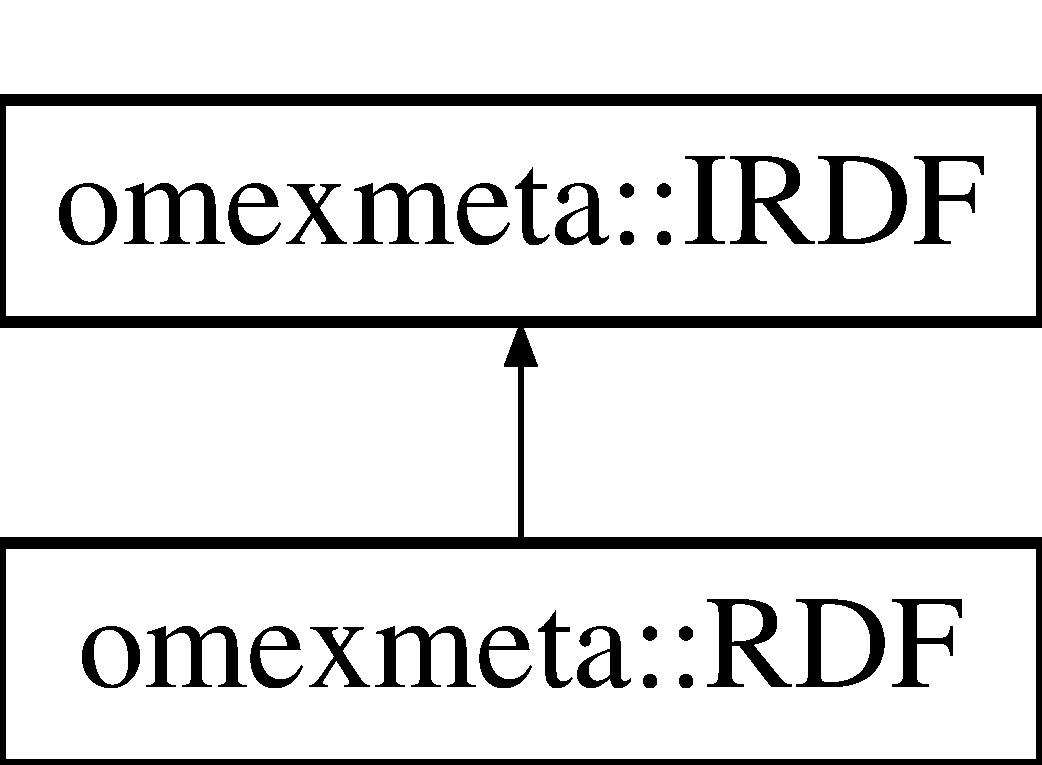
\includegraphics[height=2.000000cm]{classomexmeta_1_1RDF}
\end{center}
\end{figure}
\doxysubsection*{Public Member Functions}
\begin{DoxyCompactItemize}
\item 
\mbox{\hyperlink{classomexmeta_1_1RDF_aecb90e51830082f78ff055c045f4b439}{R\+DF}} (const std\+::string \&storage\+\_\+type=\char`\"{}memory\char`\"{}, const std\+::string \&storage\+\_\+name=\char`\"{}Semsim\+Store\char`\"{}, const char $\ast$storage\+\_\+options=nullptr, const char $\ast$model\+\_\+options=nullptr)
\begin{DoxyCompactList}\small\item\em constructor for \mbox{\hyperlink{classomexmeta_1_1RDF}{R\+DF}} class \end{DoxyCompactList}\item 
\mbox{\Hypertarget{classomexmeta_1_1RDF_a87b1eb7fe49f4928e61c399edf49e09c}\label{classomexmeta_1_1RDF_a87b1eb7fe49f4928e61c399edf49e09c}} 
\mbox{\hyperlink{classomexmeta_1_1RDF_a87b1eb7fe49f4928e61c399edf49e09c}{$\sim$\+R\+DF}} ()
\begin{DoxyCompactList}\small\item\em destructor for \mbox{\hyperlink{classomexmeta_1_1RDF}{R\+DF}} \end{DoxyCompactList}\item 
\mbox{\hyperlink{classomexmeta_1_1RDF_ad95c4a8588988efe399c7f984e304990}{R\+DF}} (const \mbox{\hyperlink{classomexmeta_1_1RDF}{R\+DF}} \&rdf)=delete
\begin{DoxyCompactList}\small\item\em copy constructor for \mbox{\hyperlink{classomexmeta_1_1RDF}{R\+DF}} class \end{DoxyCompactList}\item 
\mbox{\Hypertarget{classomexmeta_1_1RDF_a6490b2ea0d10e3026bea587a305b7fb9}\label{classomexmeta_1_1RDF_a6490b2ea0d10e3026bea587a305b7fb9}} 
\mbox{\hyperlink{classomexmeta_1_1RDF_a6490b2ea0d10e3026bea587a305b7fb9}{R\+DF}} (\mbox{\hyperlink{classomexmeta_1_1RDF}{R\+DF}} \&\&rdf) noexcept
\begin{DoxyCompactList}\small\item\em move constructor for \mbox{\hyperlink{classomexmeta_1_1RDF}{R\+DF}} class \end{DoxyCompactList}\item 
\mbox{\hyperlink{classomexmeta_1_1RDF}{R\+DF}} \& \mbox{\hyperlink{classomexmeta_1_1RDF_a9d1b20d798969d3c1dac412c621247b9}{operator=}} (const \mbox{\hyperlink{classomexmeta_1_1RDF}{R\+DF}} \&rdf)=delete
\begin{DoxyCompactList}\small\item\em copy assignment constructor for \mbox{\hyperlink{classomexmeta_1_1RDF}{R\+DF}} ojects \end{DoxyCompactList}\item 
\mbox{\Hypertarget{classomexmeta_1_1RDF_ae3739bda3be0986547c31559381f3df4}\label{classomexmeta_1_1RDF_ae3739bda3be0986547c31559381f3df4}} 
\mbox{\hyperlink{classomexmeta_1_1RDF}{R\+DF}} \& \mbox{\hyperlink{classomexmeta_1_1RDF_ae3739bda3be0986547c31559381f3df4}{operator=}} (\mbox{\hyperlink{classomexmeta_1_1RDF}{R\+DF}} \&\&rdf) noexcept
\begin{DoxyCompactList}\small\item\em move assignment operator for \mbox{\hyperlink{classomexmeta_1_1RDF}{R\+DF}} \end{DoxyCompactList}\item 
\mbox{\Hypertarget{classomexmeta_1_1RDF_a1ebd37b6dbce97660ed48031686d7f30}\label{classomexmeta_1_1RDF_a1ebd37b6dbce97660ed48031686d7f30}} 
int \mbox{\hyperlink{classomexmeta_1_1RDF_a1ebd37b6dbce97660ed48031686d7f30}{size}} () const override
\begin{DoxyCompactList}\small\item\em returns the number of triples currently present in the \mbox{\hyperlink{classomexmeta_1_1RDF}{R\+DF}} graph. \end{DoxyCompactList}\item 
bool \mbox{\hyperlink{classomexmeta_1_1RDF_a6d8ab2edd8f798006ee77a4202bf462e}{empty}} () const override
\begin{DoxyCompactList}\small\item\em indicator for whether the \mbox{\hyperlink{classomexmeta_1_1RDF}{R\+DF}} graph is empty \end{DoxyCompactList}\item 
\mbox{\Hypertarget{classomexmeta_1_1RDF_ad403d7c62ef1cf902fcb8b65c5ad641f}\label{classomexmeta_1_1RDF_ad403d7c62ef1cf902fcb8b65c5ad641f}} 
void \mbox{\hyperlink{classomexmeta_1_1RDF_ad403d7c62ef1cf902fcb8b65c5ad641f}{add\+From\+String}} (const std\+::string \&str, const std\+::string \&syntax=\char`\"{}guess\char`\"{}) override
\begin{DoxyCompactList}\small\item\em non-\/static variant of \mbox{\hyperlink{classomexmeta_1_1RDF_ab282cd4a6d76e87fa9ca91077936eeb5}{R\+D\+F\+::from\+String()}}. Reads rdf into an \mbox{\hyperlink{classomexmeta_1_1RDF}{R\+DF}} instance. See \mbox{\hyperlink{classomexmeta_1_1RDF_ab282cd4a6d76e87fa9ca91077936eeb5}{R\+D\+F\+::from\+String()}} for argument requirements. \end{DoxyCompactList}\item 
void \mbox{\hyperlink{classomexmeta_1_1RDF_a602c7ca8ca94b151dd97b8a513cef0a4}{add\+From\+Uri}} (const std\+::string \&uri\+\_\+string, const std\+::string \&syntax=\char`\"{}guess\char`\"{}) override
\begin{DoxyCompactList}\small\item\em non-\/static counterpart of \mbox{\hyperlink{classomexmeta_1_1RDF_a18f57a8d85f89ff7b0575540ab280a2f}{R\+D\+F\+::from\+Uri}}. Downloads and parses rdf from a U\+RI. \end{DoxyCompactList}\item 
void \mbox{\hyperlink{classomexmeta_1_1RDF_af62debd6edc14e6ff06c28d7726cfef4}{add\+From\+File}} (const std\+::string \&filename, const std\+::string \&syntax) override
\begin{DoxyCompactList}\small\item\em non-\/static counter part of \mbox{\hyperlink{classomexmeta_1_1RDF_a87ab63ef63126945d345d463e0a14f5e}{R\+D\+F\+::from\+File}}. Reads rdf from annotations in a file \end{DoxyCompactList}\item 
std\+::string \mbox{\hyperlink{classomexmeta_1_1RDF_a1fa12a4283c03d068f03ae33c5114c54}{to\+String}} (const std\+::string \&syntax=\char`\"{}turtle\char`\"{}, const char $\ast$mime\+\_\+type=nullptr, const char $\ast$type\+\_\+uri=nullptr) override
\begin{DoxyCompactList}\small\item\em serialize \mbox{\hyperlink{classomexmeta_1_1RDF}{R\+DF}} graph to string \end{DoxyCompactList}\item 
void \mbox{\hyperlink{classomexmeta_1_1RDF_a3ca48d8b9790b4ccd091204c4d9a0c05}{to\+File}} (const std\+::string \&filename, const std\+::string \&syntax=\char`\"{}turtle\char`\"{}, const char $\ast$mime\+\_\+type=nullptr, const char $\ast$type\+\_\+uri=nullptr) override
\begin{DoxyCompactList}\small\item\em Write annotations to file. \end{DoxyCompactList}\item 
\mbox{\hyperlink{classomexmeta_1_1Editor}{Editor}} \mbox{\hyperlink{classomexmeta_1_1RDF_a99bf8d2fd11cc200501ead29f4a8656f}{to\+Editor}} (const std\+::string \&xml, bool generate\+\_\+new\+\_\+metaids=false, bool sbml\+\_\+semantic\+\_\+extraction=true) override
\begin{DoxyCompactList}\small\item\em instantiate an \mbox{\hyperlink{classomexmeta_1_1Editor}{Editor}} object. \end{DoxyCompactList}\item 
\mbox{\Hypertarget{classomexmeta_1_1RDF_a072496a750958bd7c59471bb5229f0bb}\label{classomexmeta_1_1RDF_a072496a750958bd7c59471bb5229f0bb}} 
\mbox{\hyperlink{classomexmeta_1_1Editor}{Editor}} $\ast$ {\bfseries to\+Editor\+Ptr} (const std\+::string \&xml, bool generate\+\_\+new\+\_\+metaids=false, bool sbml\+\_\+semantic\+\_\+extraction=true) override
\item 
\mbox{\Hypertarget{classomexmeta_1_1RDF_a081395bf83bcbbbf7b1ca5df10642b5e}\label{classomexmeta_1_1RDF_a081395bf83bcbbbf7b1ca5df10642b5e}} 
librdf\+\_\+model $\ast$ {\bfseries get\+Model} () const override
\item 
\mbox{\Hypertarget{classomexmeta_1_1RDF_aa143aa353145b64fd6e715ae83fe40af}\label{classomexmeta_1_1RDF_aa143aa353145b64fd6e715ae83fe40af}} 
librdf\+\_\+storage $\ast$ {\bfseries get\+Storage} () const override
\item 
\mbox{\Hypertarget{classomexmeta_1_1RDF_ab833a4b13d27b5c7e3667dcfe2937e98}\label{classomexmeta_1_1RDF_ab833a4b13d27b5c7e3667dcfe2937e98}} 
int {\bfseries commit\+Transaction} () const override
\item 
\mbox{\Hypertarget{classomexmeta_1_1RDF_a6a9df7e508c0a516e793614e12771759}\label{classomexmeta_1_1RDF_a6a9df7e508c0a516e793614e12771759}} 
int {\bfseries start\+Transaction} () const override
\item 
\mbox{\Hypertarget{classomexmeta_1_1RDF_a752cdbce8114f3bb9b39734c263ac98b}\label{classomexmeta_1_1RDF_a752cdbce8114f3bb9b39734c263ac98b}} 
void $\ast$ {\bfseries get\+Transaction\+Handle} () const override
\item 
\mbox{\Hypertarget{classomexmeta_1_1RDF_a8962e4cfd044a0a76fc09f35d125c40a}\label{classomexmeta_1_1RDF_a8962e4cfd044a0a76fc09f35d125c40a}} 
int {\bfseries start\+Transaction\+With\+Handle} (void $\ast$handle) const override
\item 
\mbox{\Hypertarget{classomexmeta_1_1RDF_a3fd8f1647bbe570d1f4efdffe378d624}\label{classomexmeta_1_1RDF_a3fd8f1647bbe570d1f4efdffe378d624}} 
int {\bfseries get\+Transaction\+Rollback} () const override
\item 
\mbox{\Hypertarget{classomexmeta_1_1RDF_a6b6244dac65b1cdfab6f450646c857b6}\label{classomexmeta_1_1RDF_a6b6244dac65b1cdfab6f450646c857b6}} 
std\+::string {\bfseries query\+Results\+As\+String} (const std\+::string \&query\+\_\+str, const std\+::string \&results\+\_\+syntax) const override
\item 
\mbox{\Hypertarget{classomexmeta_1_1RDF_a44015b8feae5e1b8f816501f44530732}\label{classomexmeta_1_1RDF_a44015b8feae5e1b8f816501f44530732}} 
Results\+Map {\bfseries query\+Results\+As\+Map} (const std\+::string \&query\+\_\+str) const override
\item 
std\+::unordered\+\_\+map$<$ std\+::string, std\+::string $>$ \mbox{\hyperlink{classomexmeta_1_1RDF_a867deb1681500712e942b61e4e1460c6}{propagate\+Namespaces\+From\+Parser}} (const std\+::vector$<$ std\+::string $>$ \&seen\+\_\+namespaces) override
\begin{DoxyCompactList}\small\item\em compared namespaces seen with namespaces known and ensures models that use a known namespace use that namespace. \end{DoxyCompactList}\item 
Omex\+Meta\+Xml\+Type \mbox{\hyperlink{classomexmeta_1_1RDF_a501c173fc1b60932391f5f7a3ff8212e}{get\+Xml\+Type}} () const override
\begin{DoxyCompactList}\small\item\em getter for xml\+Type attribue. \end{DoxyCompactList}\item 
\mbox{\Hypertarget{classomexmeta_1_1RDF_add69d33d544dc31789b2ff0a71182a84}\label{classomexmeta_1_1RDF_add69d33d544dc31789b2ff0a71182a84}} 
bool {\bfseries operator==} (const \mbox{\hyperlink{classomexmeta_1_1RDF}{R\+DF}} \&rhs) const
\item 
\mbox{\Hypertarget{classomexmeta_1_1RDF_ac652b39964477c8ea69e5218f2203013}\label{classomexmeta_1_1RDF_ac652b39964477c8ea69e5218f2203013}} 
bool {\bfseries operator!=} (const \mbox{\hyperlink{classomexmeta_1_1RDF}{R\+DF}} \&rhs) const
\item 
void \mbox{\hyperlink{classomexmeta_1_1RDF_a72705a830be2b6d6ed40d2cb65136335}{set\+Xml\+Type}} (Omex\+Meta\+Xml\+Type xml\+Type) override
\begin{DoxyCompactList}\small\item\em set the xml type for the current graph. \end{DoxyCompactList}\item 
\mbox{\Hypertarget{classomexmeta_1_1RDF_ae4ba9a6a862c4acce2f6757a99b4c4c2}\label{classomexmeta_1_1RDF_ae4ba9a6a862c4acce2f6757a99b4c4c2}} 
const std\+::string \& \mbox{\hyperlink{classomexmeta_1_1RDF_ae4ba9a6a862c4acce2f6757a99b4c4c2}{get\+Repository\+Uri}} () const override
\begin{DoxyCompactList}\small\item\em getter for repository uri which defaults to \char`\"{}http\+://omex-\/library.\+org/\char`\"{} \end{DoxyCompactList}\item 
void \mbox{\hyperlink{classomexmeta_1_1RDF_a9f35a52ca041be0f036197989cdca3e7}{set\+Repository\+Uri}} (const std\+::string \&repository\+Name) override
\begin{DoxyCompactList}\small\item\em setter for the repository uri which defaults to \char`\"{}http\+://omex-\/library.\+org/\char`\"{}. \end{DoxyCompactList}\item 
const std\+::string \& \mbox{\hyperlink{classomexmeta_1_1RDF_a6cba8783aa84a3df928825ce44555733}{get\+Archive\+Uri}} () const override
\begin{DoxyCompactList}\small\item\em getter for archive\+Uri attribute. \end{DoxyCompactList}\item 
void \mbox{\hyperlink{classomexmeta_1_1RDF_aabb921ecd37e3e9fc0e29066b658bf59}{set\+Archive\+Uri}} (const std\+::string \&archive\+Name) override
\begin{DoxyCompactList}\small\item\em setter for archive\+Uri attribute. \end{DoxyCompactList}\item 
const std\+::string \& \mbox{\hyperlink{classomexmeta_1_1RDF_a0529edb78dde0798541cdc9761e2a0e7}{get\+Model\+Uri}} () const override
\begin{DoxyCompactList}\small\item\em getter for model uri. \end{DoxyCompactList}\item 
void \mbox{\hyperlink{classomexmeta_1_1RDF_a0c6ec28bb9cd9730224331ed69d41cad}{set\+Model\+Uri}} (std\+::string model\+Name) override
\begin{DoxyCompactList}\small\item\em setter for model uri. \end{DoxyCompactList}\item 
const std\+::string \& \mbox{\hyperlink{classomexmeta_1_1RDF_a7399a80108553b138bf168a76f8a4adf}{get\+Local\+Uri}} () const override
\begin{DoxyCompactList}\small\item\em getter for local uri attribute. \end{DoxyCompactList}\item 
\mbox{\Hypertarget{classomexmeta_1_1RDF_ab6b74c206a0b9cbce946f9d7bd8d1f56}\label{classomexmeta_1_1RDF_ab6b74c206a0b9cbce946f9d7bd8d1f56}} 
void \mbox{\hyperlink{classomexmeta_1_1RDF_ab6b74c206a0b9cbce946f9d7bd8d1f56}{add\+Triple}} (const \mbox{\hyperlink{classomexmeta_1_1Triple}{Triple}} \&triple) override
\begin{DoxyCompactList}\small\item\em add a \mbox{\hyperlink{classomexmeta_1_1Triple}{Triple}} to the current model \end{DoxyCompactList}\item 
\mbox{\Hypertarget{classomexmeta_1_1RDF_aa8f640de046b3c1bd43de0fe5aba0958}\label{classomexmeta_1_1RDF_aa8f640de046b3c1bd43de0fe5aba0958}} 
void \mbox{\hyperlink{classomexmeta_1_1RDF_aa8f640de046b3c1bd43de0fe5aba0958}{add\+Triples}} (\mbox{\hyperlink{classomexmeta_1_1Triples}{Triples}} \&triples) override
\begin{DoxyCompactList}\small\item\em add a set of \mbox{\hyperlink{classomexmeta_1_1Triples}{Triples}} to the current model \end{DoxyCompactList}\item 
\mbox{\Hypertarget{classomexmeta_1_1RDF_a9565b7c0ad81abed2243c0a76f1ebea3}\label{classomexmeta_1_1RDF_a9565b7c0ad81abed2243c0a76f1ebea3}} 
\mbox{\hyperlink{classomexmeta_1_1UriHandler}{Uri\+Handler}} \& {\bfseries get\+Uri\+Handler} () override
\end{DoxyCompactItemize}
\doxysubsection*{Static Public Member Functions}
\begin{DoxyCompactItemize}
\item 
static \mbox{\hyperlink{classomexmeta_1_1RDF}{R\+DF}} \mbox{\hyperlink{classomexmeta_1_1RDF_ab282cd4a6d76e87fa9ca91077936eeb5}{from\+String}} (const std\+::string \&str, const std\+::string \&syntax=\char`\"{}guess\char`\"{})
\begin{DoxyCompactList}\small\item\em instantiate an \mbox{\hyperlink{classomexmeta_1_1RDF}{R\+DF}} instance and read annotations from a string. \mbox{\hyperlink{classThis}{This}} is a static method. \end{DoxyCompactList}\item 
static \mbox{\hyperlink{classomexmeta_1_1RDF}{R\+DF}} \mbox{\hyperlink{classomexmeta_1_1RDF_a18f57a8d85f89ff7b0575540ab280a2f}{from\+Uri}} (const std\+::string \&uri\+\_\+string, const std\+::string \&syntax=\char`\"{}guess\char`\"{})
\begin{DoxyCompactList}\small\item\em parse \mbox{\hyperlink{classomexmeta_1_1RDF}{R\+DF}} directly from a uri \end{DoxyCompactList}\item 
static \mbox{\hyperlink{classomexmeta_1_1RDF}{R\+DF}} \mbox{\hyperlink{classomexmeta_1_1RDF_a87ab63ef63126945d345d463e0a14f5e}{from\+File}} (const std\+::string \&filename, const std\+::string \&syntax)
\begin{DoxyCompactList}\small\item\em read rdf from annotations in a file \end{DoxyCompactList}\item 
static void \mbox{\hyperlink{classomexmeta_1_1RDF_a64aad2ca67fb7b7efe175354bb78440f}{from\+String}} (\mbox{\hyperlink{classomexmeta_1_1RDF}{R\+DF}} $\ast$rdf, const std\+::string \&str, const std\+::string \&syntax, std\+::string base\+\_\+uri=\char`\"{}Annotations.\+rdf\char`\"{})
\begin{DoxyCompactList}\small\item\em non static version of \mbox{\hyperlink{classomexmeta_1_1RDF_ab282cd4a6d76e87fa9ca91077936eeb5}{R\+D\+F\+::from\+String}} that takes a $\ast$ \mbox{\hyperlink{classomexmeta_1_1RDF}{R\+DF}} pointer object and modifies in place. \end{DoxyCompactList}\item 
\mbox{\Hypertarget{classomexmeta_1_1RDF_ae01ed260e02eda2141ffe1288f78c177}\label{classomexmeta_1_1RDF_ae01ed260e02eda2141ffe1288f78c177}} 
static std\+::ostringstream {\bfseries list\+Options} ()
\item 
static bool \mbox{\hyperlink{classomexmeta_1_1RDF_a436984961a0a9881824e031b855b7413}{equals}} (\mbox{\hyperlink{classomexmeta_1_1RDF}{R\+DF}} $\ast$actual, const std\+::string \&expected, const std\+::string \&syntax=\char`\"{}turtle\char`\"{}, bool verbose=false)
\begin{DoxyCompactList}\small\item\em test for equality between \end{DoxyCompactList}\item 
static bool \mbox{\hyperlink{classomexmeta_1_1RDF_a43fa92ba852b2181e0b437c812abac7d}{equals}} (const \mbox{\hyperlink{classomexmeta_1_1Triple}{Triple}} \&actual, const std\+::string \&expected, const std\+::string \&syntax=\char`\"{}turtle\char`\"{}, bool verbose=false)
\begin{DoxyCompactList}\small\item\em test for equality between \end{DoxyCompactList}\item 
static bool \mbox{\hyperlink{classomexmeta_1_1RDF_a91068cb9e9f5f5b3295de96dbf9d243b}{equals}} (\mbox{\hyperlink{classomexmeta_1_1Triples}{Triples}} \&actual, const std\+::string \&expected, const std\+::string \&syntax=\char`\"{}turtle\char`\"{}, bool verbose=false)
\begin{DoxyCompactList}\small\item\em test for equality between \end{DoxyCompactList}\item 
static bool \mbox{\hyperlink{classomexmeta_1_1RDF_a60d25001511fbde99b4ca802d8e7621c}{equals}} (\mbox{\hyperlink{classomexmeta_1_1RDF}{R\+DF}} $\ast$actual, \mbox{\hyperlink{classomexmeta_1_1RDF}{R\+DF}} $\ast$expected, const std\+::string \&syntax=\char`\"{}turtle\char`\"{}, bool verbose=false)
\begin{DoxyCompactList}\small\item\em test for equality between \end{DoxyCompactList}\item 
static bool \mbox{\hyperlink{classomexmeta_1_1RDF_a1ec9f1e100bd55b556065856f1def174}{equals}} (const std\+::string \&first, const std\+::string \&second, const std\+::string \&first\+\_\+syntax=\char`\"{}turtle\char`\"{}, const std\+::string \&second\+\_\+syntax=\char`\"{}turtle\char`\"{}, bool verbose=false)
\begin{DoxyCompactList}\small\item\em test for equality between \end{DoxyCompactList}\end{DoxyCompactItemize}
\doxysubsection*{Public Attributes}
\begin{DoxyCompactItemize}
\item 
Namespace\+Map \mbox{\hyperlink{classomexmeta_1_1RDF_a1979d7d70a4c20f2e63f00c7fa668b1f}{namespaces\+\_\+}}
\item 
std\+::vector$<$ std\+::string $>$ \mbox{\hyperlink{classomexmeta_1_1RDF_a82bc53feb93e1243970400fd104174da}{seen\+\_\+namespaces\+\_\+}}
\item 
\mbox{\Hypertarget{classomexmeta_1_1RDF_a59014bbb45a43dbfa760480f1713c473}\label{classomexmeta_1_1RDF_a59014bbb45a43dbfa760480f1713c473}} 
const std\+::string {\bfseries O\+M\+E\+Xlib\+\_\+} = \char`\"{}http\+://O\+M\+E\+Xlibrary.\+org/\char`\"{}
\end{DoxyCompactItemize}


\doxysubsection{Constructor \& Destructor Documentation}
\mbox{\Hypertarget{classomexmeta_1_1RDF_aecb90e51830082f78ff055c045f4b439}\label{classomexmeta_1_1RDF_aecb90e51830082f78ff055c045f4b439}} 
\index{omexmeta::RDF@{omexmeta::RDF}!RDF@{RDF}}
\index{RDF@{RDF}!omexmeta::RDF@{omexmeta::RDF}}
\doxysubsubsection{\texorpdfstring{RDF()}{RDF()}\hspace{0.1cm}{\footnotesize\ttfamily [1/2]}}
{\footnotesize\ttfamily omexmeta\+::\+R\+D\+F\+::\+R\+DF (\begin{DoxyParamCaption}\item[{const std\+::string \&}]{storage\+\_\+type = {\ttfamily \char`\"{}memory\char`\"{}},  }\item[{const std\+::string \&}]{storage\+\_\+name = {\ttfamily \char`\"{}SemsimStore\char`\"{}},  }\item[{const char $\ast$}]{storage\+\_\+options = {\ttfamily nullptr},  }\item[{const char $\ast$}]{model\+\_\+options = {\ttfamily nullptr} }\end{DoxyParamCaption})\hspace{0.3cm}{\ttfamily [explicit]}}



constructor for \mbox{\hyperlink{classomexmeta_1_1RDF}{R\+DF}} class 


\begin{DoxyParams}{Parameters}
{\em storage\+\_\+type.} & Defaults to memory. Other options include\+: \char`\"{}hashes\char`\"{}, \char`\"{}file\char`\"{}, \char`\"{}mysql\char`\"{}, \char`\"{}postgresql\char`\"{}, \char`\"{}sqlite\char`\"{}, \char`\"{}uri\char`\"{}, \\
\hline
{\em storage\+\_\+name} & name used for storage. When storage is not internally held in memory, this becomes the name of the file or database. \\
\hline
{\em storage\+\_\+options} & options that get passed on to storage. Please study \href{http://librdf.org/docs/api/redland-storage-modules.html}{\texttt{ http\+://librdf.\+org/docs/api/redland-\/storage-\/modules.\+html}} for more information. @model\+\_\+options options that get passed to the model. Please see \href{http://librdf.org/docs/api/index.html}{\texttt{ http\+://librdf.\+org/docs/api/index.\+html}} for more details. \\
\hline
\end{DoxyParams}
\mbox{\Hypertarget{classomexmeta_1_1RDF_ad95c4a8588988efe399c7f984e304990}\label{classomexmeta_1_1RDF_ad95c4a8588988efe399c7f984e304990}} 
\index{omexmeta::RDF@{omexmeta::RDF}!RDF@{RDF}}
\index{RDF@{RDF}!omexmeta::RDF@{omexmeta::RDF}}
\doxysubsubsection{\texorpdfstring{RDF()}{RDF()}\hspace{0.1cm}{\footnotesize\ttfamily [2/2]}}
{\footnotesize\ttfamily omexmeta\+::\+R\+D\+F\+::\+R\+DF (\begin{DoxyParamCaption}\item[{const \mbox{\hyperlink{classomexmeta_1_1RDF}{R\+DF}} \&}]{rdf }\end{DoxyParamCaption})\hspace{0.3cm}{\ttfamily [delete]}}



copy constructor for \mbox{\hyperlink{classomexmeta_1_1RDF}{R\+DF}} class 

\mbox{\hyperlink{classomexmeta_1_1RDF}{R\+DF}} instances are not copyable due to restrictions within the redland libraries. You must instead move \mbox{\hyperlink{classomexmeta_1_1RDF}{R\+DF}} objects. 

\doxysubsection{Member Function Documentation}
\mbox{\Hypertarget{classomexmeta_1_1RDF_af62debd6edc14e6ff06c28d7726cfef4}\label{classomexmeta_1_1RDF_af62debd6edc14e6ff06c28d7726cfef4}} 
\index{omexmeta::RDF@{omexmeta::RDF}!addFromFile@{addFromFile}}
\index{addFromFile@{addFromFile}!omexmeta::RDF@{omexmeta::RDF}}
\doxysubsubsection{\texorpdfstring{addFromFile()}{addFromFile()}}
{\footnotesize\ttfamily void omexmeta\+::\+R\+D\+F\+::add\+From\+File (\begin{DoxyParamCaption}\item[{const std\+::string \&}]{filename,  }\item[{const std\+::string \&}]{syntax }\end{DoxyParamCaption})\hspace{0.3cm}{\ttfamily [override]}, {\ttfamily [virtual]}}



non-\/static counter part of \mbox{\hyperlink{classomexmeta_1_1RDF_a87ab63ef63126945d345d463e0a14f5e}{R\+D\+F\+::from\+File}}. Reads rdf from annotations in a file 


\begin{DoxyParams}{Parameters}
{\em filename} & the filename to read as string \\
\hline
{\em syntax} & the syntax of the \mbox{\hyperlink{classomexmeta_1_1RDF}{R\+DF}} in filename \\
\hline
\end{DoxyParams}
\begin{DoxyReturn}{Returns}
an instantiated \mbox{\hyperlink{classomexmeta_1_1RDF}{R\+DF}} object  Uses Librdf\+Parser\+::from\+File under the hood 
\end{DoxyReturn}


Implements \mbox{\hyperlink{classomexmeta_1_1IRDF}{omexmeta\+::\+I\+R\+DF}}.

\mbox{\Hypertarget{classomexmeta_1_1RDF_a602c7ca8ca94b151dd97b8a513cef0a4}\label{classomexmeta_1_1RDF_a602c7ca8ca94b151dd97b8a513cef0a4}} 
\index{omexmeta::RDF@{omexmeta::RDF}!addFromUri@{addFromUri}}
\index{addFromUri@{addFromUri}!omexmeta::RDF@{omexmeta::RDF}}
\doxysubsubsection{\texorpdfstring{addFromUri()}{addFromUri()}}
{\footnotesize\ttfamily void omexmeta\+::\+R\+D\+F\+::add\+From\+Uri (\begin{DoxyParamCaption}\item[{const std\+::string \&}]{uri\+\_\+string,  }\item[{const std\+::string \&}]{syntax = {\ttfamily \char`\"{}guess\char`\"{}} }\end{DoxyParamCaption})\hspace{0.3cm}{\ttfamily [override]}, {\ttfamily [virtual]}}



non-\/static counterpart of \mbox{\hyperlink{classomexmeta_1_1RDF_a18f57a8d85f89ff7b0575540ab280a2f}{R\+D\+F\+::from\+Uri}}. Downloads and parses rdf from a U\+RI. 

See \mbox{\hyperlink{classomexmeta_1_1RDF_a18f57a8d85f89ff7b0575540ab280a2f}{R\+D\+F\+::from\+Uri}} for details. 

Implements \mbox{\hyperlink{classomexmeta_1_1IRDF}{omexmeta\+::\+I\+R\+DF}}.

\mbox{\Hypertarget{classomexmeta_1_1RDF_a6d8ab2edd8f798006ee77a4202bf462e}\label{classomexmeta_1_1RDF_a6d8ab2edd8f798006ee77a4202bf462e}} 
\index{omexmeta::RDF@{omexmeta::RDF}!empty@{empty}}
\index{empty@{empty}!omexmeta::RDF@{omexmeta::RDF}}
\doxysubsubsection{\texorpdfstring{empty()}{empty()}}
{\footnotesize\ttfamily bool omexmeta\+::\+R\+D\+F\+::empty (\begin{DoxyParamCaption}{ }\end{DoxyParamCaption}) const\hspace{0.3cm}{\ttfamily [override]}, {\ttfamily [virtual]}}



indicator for whether the \mbox{\hyperlink{classomexmeta_1_1RDF}{R\+DF}} graph is empty 

\begin{DoxyReturn}{Returns}
true if \mbox{\hyperlink{classomexmeta_1_1RDF}{R\+DF}} graph has no triples, false otherwise. 
\end{DoxyReturn}


Implements \mbox{\hyperlink{classomexmeta_1_1IRDF}{omexmeta\+::\+I\+R\+DF}}.

\mbox{\Hypertarget{classomexmeta_1_1RDF_a1ec9f1e100bd55b556065856f1def174}\label{classomexmeta_1_1RDF_a1ec9f1e100bd55b556065856f1def174}} 
\index{omexmeta::RDF@{omexmeta::RDF}!equals@{equals}}
\index{equals@{equals}!omexmeta::RDF@{omexmeta::RDF}}
\doxysubsubsection{\texorpdfstring{equals()}{equals()}\hspace{0.1cm}{\footnotesize\ttfamily [1/5]}}
{\footnotesize\ttfamily bool omexmeta\+::\+R\+D\+F\+::equals (\begin{DoxyParamCaption}\item[{const std\+::string \&}]{first,  }\item[{const std\+::string \&}]{second,  }\item[{const std\+::string \&}]{first\+\_\+syntax = {\ttfamily \char`\"{}turtle\char`\"{}},  }\item[{const std\+::string \&}]{second\+\_\+syntax = {\ttfamily \char`\"{}turtle\char`\"{}},  }\item[{bool}]{verbose = {\ttfamily false} }\end{DoxyParamCaption})\hspace{0.3cm}{\ttfamily [static]}}



test for equality between 


\begin{DoxyParams}{Parameters}
{\em first} & and\\
\hline
{\em second} & \\
\hline
\end{DoxyParams}
\mbox{\Hypertarget{classomexmeta_1_1RDF_a43fa92ba852b2181e0b437c812abac7d}\label{classomexmeta_1_1RDF_a43fa92ba852b2181e0b437c812abac7d}} 
\index{omexmeta::RDF@{omexmeta::RDF}!equals@{equals}}
\index{equals@{equals}!omexmeta::RDF@{omexmeta::RDF}}
\doxysubsubsection{\texorpdfstring{equals()}{equals()}\hspace{0.1cm}{\footnotesize\ttfamily [2/5]}}
{\footnotesize\ttfamily bool omexmeta\+::\+R\+D\+F\+::equals (\begin{DoxyParamCaption}\item[{const \mbox{\hyperlink{classomexmeta_1_1Triple}{Triple}} \&}]{actual,  }\item[{const std\+::string \&}]{expected,  }\item[{const std\+::string \&}]{syntax = {\ttfamily \char`\"{}turtle\char`\"{}},  }\item[{bool}]{verbose = {\ttfamily false} }\end{DoxyParamCaption})\hspace{0.3cm}{\ttfamily [static]}}



test for equality between 


\begin{DoxyParams}{Parameters}
{\em actual} & and\\
\hline
{\em expected} & \\
\hline
\end{DoxyParams}
\mbox{\Hypertarget{classomexmeta_1_1RDF_a436984961a0a9881824e031b855b7413}\label{classomexmeta_1_1RDF_a436984961a0a9881824e031b855b7413}} 
\index{omexmeta::RDF@{omexmeta::RDF}!equals@{equals}}
\index{equals@{equals}!omexmeta::RDF@{omexmeta::RDF}}
\doxysubsubsection{\texorpdfstring{equals()}{equals()}\hspace{0.1cm}{\footnotesize\ttfamily [3/5]}}
{\footnotesize\ttfamily bool omexmeta\+::\+R\+D\+F\+::equals (\begin{DoxyParamCaption}\item[{\mbox{\hyperlink{classomexmeta_1_1RDF}{R\+DF}} $\ast$}]{actual,  }\item[{const std\+::string \&}]{expected,  }\item[{const std\+::string \&}]{syntax = {\ttfamily \char`\"{}turtle\char`\"{}},  }\item[{bool}]{verbose = {\ttfamily false} }\end{DoxyParamCaption})\hspace{0.3cm}{\ttfamily [static]}}



test for equality between 


\begin{DoxyParams}{Parameters}
{\em actual} & and\\
\hline
{\em expected} & \\
\hline
\end{DoxyParams}
\mbox{\Hypertarget{classomexmeta_1_1RDF_a60d25001511fbde99b4ca802d8e7621c}\label{classomexmeta_1_1RDF_a60d25001511fbde99b4ca802d8e7621c}} 
\index{omexmeta::RDF@{omexmeta::RDF}!equals@{equals}}
\index{equals@{equals}!omexmeta::RDF@{omexmeta::RDF}}
\doxysubsubsection{\texorpdfstring{equals()}{equals()}\hspace{0.1cm}{\footnotesize\ttfamily [4/5]}}
{\footnotesize\ttfamily bool omexmeta\+::\+R\+D\+F\+::equals (\begin{DoxyParamCaption}\item[{\mbox{\hyperlink{classomexmeta_1_1RDF}{R\+DF}} $\ast$}]{actual,  }\item[{\mbox{\hyperlink{classomexmeta_1_1RDF}{R\+DF}} $\ast$}]{expected,  }\item[{const std\+::string \&}]{syntax = {\ttfamily \char`\"{}turtle\char`\"{}},  }\item[{bool}]{verbose = {\ttfamily false} }\end{DoxyParamCaption})\hspace{0.3cm}{\ttfamily [static]}}



test for equality between 


\begin{DoxyParams}{Parameters}
{\em actual} & and\\
\hline
{\em expected} & \\
\hline
\end{DoxyParams}
\mbox{\Hypertarget{classomexmeta_1_1RDF_a91068cb9e9f5f5b3295de96dbf9d243b}\label{classomexmeta_1_1RDF_a91068cb9e9f5f5b3295de96dbf9d243b}} 
\index{omexmeta::RDF@{omexmeta::RDF}!equals@{equals}}
\index{equals@{equals}!omexmeta::RDF@{omexmeta::RDF}}
\doxysubsubsection{\texorpdfstring{equals()}{equals()}\hspace{0.1cm}{\footnotesize\ttfamily [5/5]}}
{\footnotesize\ttfamily bool omexmeta\+::\+R\+D\+F\+::equals (\begin{DoxyParamCaption}\item[{\mbox{\hyperlink{classomexmeta_1_1Triples}{Triples}} \&}]{actual,  }\item[{const std\+::string \&}]{expected,  }\item[{const std\+::string \&}]{syntax = {\ttfamily \char`\"{}turtle\char`\"{}},  }\item[{bool}]{verbose = {\ttfamily false} }\end{DoxyParamCaption})\hspace{0.3cm}{\ttfamily [static]}}



test for equality between 


\begin{DoxyParams}{Parameters}
{\em actual} & and\\
\hline
{\em expected} & \\
\hline
\end{DoxyParams}
\mbox{\Hypertarget{classomexmeta_1_1RDF_a87ab63ef63126945d345d463e0a14f5e}\label{classomexmeta_1_1RDF_a87ab63ef63126945d345d463e0a14f5e}} 
\index{omexmeta::RDF@{omexmeta::RDF}!fromFile@{fromFile}}
\index{fromFile@{fromFile}!omexmeta::RDF@{omexmeta::RDF}}
\doxysubsubsection{\texorpdfstring{fromFile()}{fromFile()}}
{\footnotesize\ttfamily \mbox{\hyperlink{classomexmeta_1_1RDF}{R\+DF}} omexmeta\+::\+R\+D\+F\+::from\+File (\begin{DoxyParamCaption}\item[{const std\+::string \&}]{filename,  }\item[{const std\+::string \&}]{syntax }\end{DoxyParamCaption})\hspace{0.3cm}{\ttfamily [static]}}



read rdf from annotations in a file 


\begin{DoxyParams}{Parameters}
{\em filename} & the filename to read as string \\
\hline
{\em syntax} & the syntax of the \mbox{\hyperlink{classomexmeta_1_1RDF}{R\+DF}} in filename \\
\hline
\end{DoxyParams}
\begin{DoxyReturn}{Returns}
an instantiated \mbox{\hyperlink{classomexmeta_1_1RDF}{R\+DF}} object  Uses Librdf\+Parser\+::from\+File under the hood 
\end{DoxyReturn}
\mbox{\Hypertarget{classomexmeta_1_1RDF_ab282cd4a6d76e87fa9ca91077936eeb5}\label{classomexmeta_1_1RDF_ab282cd4a6d76e87fa9ca91077936eeb5}} 
\index{omexmeta::RDF@{omexmeta::RDF}!fromString@{fromString}}
\index{fromString@{fromString}!omexmeta::RDF@{omexmeta::RDF}}
\doxysubsubsection{\texorpdfstring{fromString()}{fromString()}\hspace{0.1cm}{\footnotesize\ttfamily [1/2]}}
{\footnotesize\ttfamily \mbox{\hyperlink{classomexmeta_1_1RDF}{R\+DF}} omexmeta\+::\+R\+D\+F\+::from\+String (\begin{DoxyParamCaption}\item[{const std\+::string \&}]{str,  }\item[{const std\+::string \&}]{syntax = {\ttfamily \char`\"{}guess\char`\"{}} }\end{DoxyParamCaption})\hspace{0.3cm}{\ttfamily [static]}}



instantiate an \mbox{\hyperlink{classomexmeta_1_1RDF}{R\+DF}} instance and read annotations from a string. \mbox{\hyperlink{classThis}{This}} is a static method. 


\begin{DoxyParams}{Parameters}
{\em str} & a reference to the string containing annotations \\
\hline
{\em syntax} & which syntax str is in. Default=\char`\"{}guess\char`\"{} \+: try to guess. \\
\hline
\end{DoxyParams}
\mbox{\Hypertarget{classomexmeta_1_1RDF_a64aad2ca67fb7b7efe175354bb78440f}\label{classomexmeta_1_1RDF_a64aad2ca67fb7b7efe175354bb78440f}} 
\index{omexmeta::RDF@{omexmeta::RDF}!fromString@{fromString}}
\index{fromString@{fromString}!omexmeta::RDF@{omexmeta::RDF}}
\doxysubsubsection{\texorpdfstring{fromString()}{fromString()}\hspace{0.1cm}{\footnotesize\ttfamily [2/2]}}
{\footnotesize\ttfamily void omexmeta\+::\+R\+D\+F\+::from\+String (\begin{DoxyParamCaption}\item[{\mbox{\hyperlink{classomexmeta_1_1RDF}{R\+DF}} $\ast$}]{rdf,  }\item[{const std\+::string \&}]{str,  }\item[{const std\+::string \&}]{syntax,  }\item[{std\+::string}]{base\+\_\+uri = {\ttfamily \char`\"{}Annotations.rdf\char`\"{}} }\end{DoxyParamCaption})\hspace{0.3cm}{\ttfamily [static]}}



non static version of \mbox{\hyperlink{classomexmeta_1_1RDF_ab282cd4a6d76e87fa9ca91077936eeb5}{R\+D\+F\+::from\+String}} that takes a $\ast$ \mbox{\hyperlink{classomexmeta_1_1RDF}{R\+DF}} pointer object and modifies in place. 

Primarily used for C A\+PI For developers\+: look into replacing this function fully with \mbox{\hyperlink{classomexmeta_1_1RDF_ad403d7c62ef1cf902fcb8b65c5ad641f}{R\+D\+F\+::add\+From\+String()}} method.

todo test whether deleting this method breaks any tests. if not, delete. \mbox{\Hypertarget{classomexmeta_1_1RDF_a18f57a8d85f89ff7b0575540ab280a2f}\label{classomexmeta_1_1RDF_a18f57a8d85f89ff7b0575540ab280a2f}} 
\index{omexmeta::RDF@{omexmeta::RDF}!fromUri@{fromUri}}
\index{fromUri@{fromUri}!omexmeta::RDF@{omexmeta::RDF}}
\doxysubsubsection{\texorpdfstring{fromUri()}{fromUri()}}
{\footnotesize\ttfamily \mbox{\hyperlink{classomexmeta_1_1RDF}{R\+DF}} omexmeta\+::\+R\+D\+F\+::from\+Uri (\begin{DoxyParamCaption}\item[{const std\+::string \&}]{uri\+\_\+string,  }\item[{const std\+::string \&}]{syntax = {\ttfamily \char`\"{}guess\char`\"{}} }\end{DoxyParamCaption})\hspace{0.3cm}{\ttfamily [static]}}



parse \mbox{\hyperlink{classomexmeta_1_1RDF}{R\+DF}} directly from a uri 


\begin{DoxyParams}{Parameters}
{\em uri\+\_\+string} & the uri to download containing \mbox{\hyperlink{classomexmeta_1_1RDF}{R\+DF}} \\
\hline
{\em syntax} & the syntax that the \mbox{\hyperlink{classomexmeta_1_1RDF}{R\+DF}} is in \\
\hline
\end{DoxyParams}
\begin{DoxyReturn}{Returns}
\mbox{\hyperlink{classomexmeta_1_1RDF}{R\+DF}} an instantiated \mbox{\hyperlink{classomexmeta_1_1RDF}{R\+DF}} object.
\end{DoxyReturn}
downloads uri from the internet and creates an \mbox{\hyperlink{classomexmeta_1_1RDF}{R\+DF}} graph. See Librdf\+::parse\+Uri() for more details. \mbox{\Hypertarget{classomexmeta_1_1RDF_a6cba8783aa84a3df928825ce44555733}\label{classomexmeta_1_1RDF_a6cba8783aa84a3df928825ce44555733}} 
\index{omexmeta::RDF@{omexmeta::RDF}!getArchiveUri@{getArchiveUri}}
\index{getArchiveUri@{getArchiveUri}!omexmeta::RDF@{omexmeta::RDF}}
\doxysubsubsection{\texorpdfstring{getArchiveUri()}{getArchiveUri()}}
{\footnotesize\ttfamily const std\+::string \& omexmeta\+::\+R\+D\+F\+::get\+Archive\+Uri (\begin{DoxyParamCaption}{ }\end{DoxyParamCaption}) const\hspace{0.3cm}{\ttfamily [override]}, {\ttfamily [virtual]}}



getter for archive\+Uri attribute. 

default to \href{http://omex-library.org/NewOmex.omex/}{\texttt{ http\+://omex-\/library.\+org/\+New\+Omex.\+omex/}} 

Implements \mbox{\hyperlink{classomexmeta_1_1IRDF}{omexmeta\+::\+I\+R\+DF}}.

\mbox{\Hypertarget{classomexmeta_1_1RDF_a7399a80108553b138bf168a76f8a4adf}\label{classomexmeta_1_1RDF_a7399a80108553b138bf168a76f8a4adf}} 
\index{omexmeta::RDF@{omexmeta::RDF}!getLocalUri@{getLocalUri}}
\index{getLocalUri@{getLocalUri}!omexmeta::RDF@{omexmeta::RDF}}
\doxysubsubsection{\texorpdfstring{getLocalUri()}{getLocalUri()}}
{\footnotesize\ttfamily const std\+::string \& omexmeta\+::\+R\+D\+F\+::get\+Local\+Uri (\begin{DoxyParamCaption}{ }\end{DoxyParamCaption}) const\hspace{0.3cm}{\ttfamily [override]}, {\ttfamily [virtual]}}



getter for local uri attribute. 

defaults to \href{http://omex-library.org/NewOmex.omex/NewModel.rdf\#}{\texttt{ http\+://omex-\/library.\+org/\+New\+Omex.\+omex/\+New\+Model.\+rdf\#}} 

Implements \mbox{\hyperlink{classomexmeta_1_1IRDF}{omexmeta\+::\+I\+R\+DF}}.

\mbox{\Hypertarget{classomexmeta_1_1RDF_a0529edb78dde0798541cdc9761e2a0e7}\label{classomexmeta_1_1RDF_a0529edb78dde0798541cdc9761e2a0e7}} 
\index{omexmeta::RDF@{omexmeta::RDF}!getModelUri@{getModelUri}}
\index{getModelUri@{getModelUri}!omexmeta::RDF@{omexmeta::RDF}}
\doxysubsubsection{\texorpdfstring{getModelUri()}{getModelUri()}}
{\footnotesize\ttfamily const std\+::string \& omexmeta\+::\+R\+D\+F\+::get\+Model\+Uri (\begin{DoxyParamCaption}{ }\end{DoxyParamCaption}) const\hspace{0.3cm}{\ttfamily [override]}, {\ttfamily [virtual]}}



getter for model uri. 

defaults to \href{http://omex-library.org/NewOmex.omex/NewModel.xml}{\texttt{ http\+://omex-\/library.\+org/\+New\+Omex.\+omex/\+New\+Model.\+xml}} 

Implements \mbox{\hyperlink{classomexmeta_1_1IRDF}{omexmeta\+::\+I\+R\+DF}}.

\mbox{\Hypertarget{classomexmeta_1_1RDF_a501c173fc1b60932391f5f7a3ff8212e}\label{classomexmeta_1_1RDF_a501c173fc1b60932391f5f7a3ff8212e}} 
\index{omexmeta::RDF@{omexmeta::RDF}!getXmlType@{getXmlType}}
\index{getXmlType@{getXmlType}!omexmeta::RDF@{omexmeta::RDF}}
\doxysubsubsection{\texorpdfstring{getXmlType()}{getXmlType()}}
{\footnotesize\ttfamily Omex\+Meta\+Xml\+Type omexmeta\+::\+R\+D\+F\+::get\+Xml\+Type (\begin{DoxyParamCaption}{ }\end{DoxyParamCaption}) const\hspace{0.3cm}{\ttfamily [override]}, {\ttfamily [virtual]}}



getter for xml\+Type attribue. 

when the rdf graph is sbml, it will return O\+M\+E\+X\+M\+E\+T\+A\+\_\+\+T\+Y\+P\+E\+\_\+\+S\+B\+ML. When cell\+ML it will return O\+M\+E\+X\+M\+E\+T\+A\+\_\+\+T\+Y\+P\+E\+\_\+\+C\+E\+L\+L\+ML. Otherwise it is O\+M\+E\+X\+M\+E\+T\+A\+\_\+\+T\+Y\+P\+E\+\_\+\+U\+N\+K\+N\+O\+WN. 

Implements \mbox{\hyperlink{classomexmeta_1_1IRDF}{omexmeta\+::\+I\+R\+DF}}.

\mbox{\Hypertarget{classomexmeta_1_1RDF_a9d1b20d798969d3c1dac412c621247b9}\label{classomexmeta_1_1RDF_a9d1b20d798969d3c1dac412c621247b9}} 
\index{omexmeta::RDF@{omexmeta::RDF}!operator=@{operator=}}
\index{operator=@{operator=}!omexmeta::RDF@{omexmeta::RDF}}
\doxysubsubsection{\texorpdfstring{operator=()}{operator=()}}
{\footnotesize\ttfamily \mbox{\hyperlink{classomexmeta_1_1RDF}{R\+DF}}\& omexmeta\+::\+R\+D\+F\+::operator= (\begin{DoxyParamCaption}\item[{const \mbox{\hyperlink{classomexmeta_1_1RDF}{R\+DF}} \&}]{rdf }\end{DoxyParamCaption})\hspace{0.3cm}{\ttfamily [delete]}}



copy assignment constructor for \mbox{\hyperlink{classomexmeta_1_1RDF}{R\+DF}} ojects 

Copy assignment functionality is prohibited for \mbox{\hyperlink{classomexmeta_1_1RDF}{R\+DF}} objects. Use move semantics insead. \mbox{\Hypertarget{classomexmeta_1_1RDF_a867deb1681500712e942b61e4e1460c6}\label{classomexmeta_1_1RDF_a867deb1681500712e942b61e4e1460c6}} 
\index{omexmeta::RDF@{omexmeta::RDF}!propagateNamespacesFromParser@{propagateNamespacesFromParser}}
\index{propagateNamespacesFromParser@{propagateNamespacesFromParser}!omexmeta::RDF@{omexmeta::RDF}}
\doxysubsubsection{\texorpdfstring{propagateNamespacesFromParser()}{propagateNamespacesFromParser()}}
{\footnotesize\ttfamily std\+::unordered\+\_\+map$<$ std\+::string, std\+::string $>$ omexmeta\+::\+R\+D\+F\+::propagate\+Namespaces\+From\+Parser (\begin{DoxyParamCaption}\item[{const std\+::vector$<$ std\+::string $>$ \&}]{seen\+\_\+namespaces }\end{DoxyParamCaption})\hspace{0.3cm}{\ttfamily [override]}, {\ttfamily [virtual]}}



compared namespaces seen with namespaces known and ensures models that use a known namespace use that namespace. 


\begin{DoxyParams}{Parameters}
{\em seen\+\_\+namespaces} & a vector of strings of namespaces the parser has seen before. \\
\hline
\end{DoxyParams}


Implements \mbox{\hyperlink{classomexmeta_1_1IRDF}{omexmeta\+::\+I\+R\+DF}}.

\mbox{\Hypertarget{classomexmeta_1_1RDF_aabb921ecd37e3e9fc0e29066b658bf59}\label{classomexmeta_1_1RDF_aabb921ecd37e3e9fc0e29066b658bf59}} 
\index{omexmeta::RDF@{omexmeta::RDF}!setArchiveUri@{setArchiveUri}}
\index{setArchiveUri@{setArchiveUri}!omexmeta::RDF@{omexmeta::RDF}}
\doxysubsubsection{\texorpdfstring{setArchiveUri()}{setArchiveUri()}}
{\footnotesize\ttfamily void omexmeta\+::\+R\+D\+F\+::set\+Archive\+Uri (\begin{DoxyParamCaption}\item[{const std\+::string \&}]{archive\+Name }\end{DoxyParamCaption})\hspace{0.3cm}{\ttfamily [override]}, {\ttfamily [virtual]}}



setter for archive\+Uri attribute. 


\begin{DoxyParams}{Parameters}
{\em archive\+Name} & the new name for archive uri attribute  default to \href{http://omex-library.org/NewOmex.omex/}{\texttt{ http\+://omex-\/library.\+org/\+New\+Omex.\+omex/}} \\
\hline
\end{DoxyParams}


Implements \mbox{\hyperlink{classomexmeta_1_1IRDF}{omexmeta\+::\+I\+R\+DF}}.

\mbox{\Hypertarget{classomexmeta_1_1RDF_a0c6ec28bb9cd9730224331ed69d41cad}\label{classomexmeta_1_1RDF_a0c6ec28bb9cd9730224331ed69d41cad}} 
\index{omexmeta::RDF@{omexmeta::RDF}!setModelUri@{setModelUri}}
\index{setModelUri@{setModelUri}!omexmeta::RDF@{omexmeta::RDF}}
\doxysubsubsection{\texorpdfstring{setModelUri()}{setModelUri()}}
{\footnotesize\ttfamily void omexmeta\+::\+R\+D\+F\+::set\+Model\+Uri (\begin{DoxyParamCaption}\item[{std\+::string}]{model\+Name }\end{DoxyParamCaption})\hspace{0.3cm}{\ttfamily [override]}, {\ttfamily [virtual]}}



setter for model uri. 


\begin{DoxyParams}{Parameters}
{\em model\+Name} & string for new model uri.  defaults to \href{http://omex-library.org/NewOmex.omex/NewModel.xml}{\texttt{ http\+://omex-\/library.\+org/\+New\+Omex.\+omex/\+New\+Model.\+xml}} \\
\hline
\end{DoxyParams}


Implements \mbox{\hyperlink{classomexmeta_1_1IRDF}{omexmeta\+::\+I\+R\+DF}}.

\mbox{\Hypertarget{classomexmeta_1_1RDF_a9f35a52ca041be0f036197989cdca3e7}\label{classomexmeta_1_1RDF_a9f35a52ca041be0f036197989cdca3e7}} 
\index{omexmeta::RDF@{omexmeta::RDF}!setRepositoryUri@{setRepositoryUri}}
\index{setRepositoryUri@{setRepositoryUri}!omexmeta::RDF@{omexmeta::RDF}}
\doxysubsubsection{\texorpdfstring{setRepositoryUri()}{setRepositoryUri()}}
{\footnotesize\ttfamily void omexmeta\+::\+R\+D\+F\+::set\+Repository\+Uri (\begin{DoxyParamCaption}\item[{const std\+::string \&}]{repository\+Name }\end{DoxyParamCaption})\hspace{0.3cm}{\ttfamily [override]}, {\ttfamily [virtual]}}



setter for the repository uri which defaults to \char`\"{}http\+://omex-\/library.\+org/\char`\"{}. 


\begin{DoxyParams}{Parameters}
{\em repository\+Name} & the repository uri. \\
\hline
\end{DoxyParams}


Implements \mbox{\hyperlink{classomexmeta_1_1IRDF}{omexmeta\+::\+I\+R\+DF}}.

\mbox{\Hypertarget{classomexmeta_1_1RDF_a72705a830be2b6d6ed40d2cb65136335}\label{classomexmeta_1_1RDF_a72705a830be2b6d6ed40d2cb65136335}} 
\index{omexmeta::RDF@{omexmeta::RDF}!setXmlType@{setXmlType}}
\index{setXmlType@{setXmlType}!omexmeta::RDF@{omexmeta::RDF}}
\doxysubsubsection{\texorpdfstring{setXmlType()}{setXmlType()}}
{\footnotesize\ttfamily void omexmeta\+::\+R\+D\+F\+::set\+Xml\+Type (\begin{DoxyParamCaption}\item[{Omex\+Meta\+Xml\+Type}]{xml\+Type }\end{DoxyParamCaption})\hspace{0.3cm}{\ttfamily [override]}, {\ttfamily [virtual]}}



set the xml type for the current graph. 

If you have been reading from an S\+B\+ML you cannot then read from another syntax (such as cellml). 

Implements \mbox{\hyperlink{classomexmeta_1_1IRDF}{omexmeta\+::\+I\+R\+DF}}.

\mbox{\Hypertarget{classomexmeta_1_1RDF_a99bf8d2fd11cc200501ead29f4a8656f}\label{classomexmeta_1_1RDF_a99bf8d2fd11cc200501ead29f4a8656f}} 
\index{omexmeta::RDF@{omexmeta::RDF}!toEditor@{toEditor}}
\index{toEditor@{toEditor}!omexmeta::RDF@{omexmeta::RDF}}
\doxysubsubsection{\texorpdfstring{toEditor()}{toEditor()}}
{\footnotesize\ttfamily \mbox{\hyperlink{classomexmeta_1_1Editor}{Editor}} omexmeta\+::\+R\+D\+F\+::to\+Editor (\begin{DoxyParamCaption}\item[{const std\+::string \&}]{xml,  }\item[{bool}]{generate\+\_\+new\+\_\+metaids = {\ttfamily false},  }\item[{bool}]{sbml\+\_\+semantic\+\_\+extraction = {\ttfamily true} }\end{DoxyParamCaption})\hspace{0.3cm}{\ttfamily [override]}, {\ttfamily [virtual]}}



instantiate an \mbox{\hyperlink{classomexmeta_1_1Editor}{Editor}} object. 


\begin{DoxyParams}{Parameters}
{\em xml} & the xml you want to open for editing. \mbox{\hyperlink{classThis}{This}} can be any type of xml document, but S\+B\+ML and Cell\+ML are most common. \\
\hline
{\em generate\+\_\+new\+\_\+metaids} & When true, will add metaids onto a copy of the xml source code for annotation. Default = false. \\
\hline
{\em Omex\+Meta\+Xml\+Type} & an indicator enum specifying whether the xml is sbml, cellml or unknown. Default is \char`\"{}\+O\+M\+E\+X\+M\+E\+T\+A\+\_\+\+T\+Y\+P\+E\+\_\+\+N\+O\+T\+S\+E\+T\char`\"{} \\
\hline
\end{DoxyParams}


Implements \mbox{\hyperlink{classomexmeta_1_1IRDF}{omexmeta\+::\+I\+R\+DF}}.

\mbox{\Hypertarget{classomexmeta_1_1RDF_a3ca48d8b9790b4ccd091204c4d9a0c05}\label{classomexmeta_1_1RDF_a3ca48d8b9790b4ccd091204c4d9a0c05}} 
\index{omexmeta::RDF@{omexmeta::RDF}!toFile@{toFile}}
\index{toFile@{toFile}!omexmeta::RDF@{omexmeta::RDF}}
\doxysubsubsection{\texorpdfstring{toFile()}{toFile()}}
{\footnotesize\ttfamily void omexmeta\+::\+R\+D\+F\+::to\+File (\begin{DoxyParamCaption}\item[{const std\+::string \&}]{filename,  }\item[{const std\+::string \&}]{syntax = {\ttfamily \char`\"{}turtle\char`\"{}},  }\item[{const char $\ast$}]{mime\+\_\+type = {\ttfamily nullptr},  }\item[{const char $\ast$}]{type\+\_\+uri = {\ttfamily nullptr} }\end{DoxyParamCaption})\hspace{0.3cm}{\ttfamily [override]}, {\ttfamily [virtual]}}



Write annotations to file. 


\begin{DoxyParams}{Parameters}
{\em syntax} & the expected output syntax. Options include\+: \char`\"{}ntriples\char`\"{}, \char`\"{}turtle\char`\"{}, \char`\"{}rdfxml-\/xmp\char`\"{}, \char`\"{}rdfxml-\/abbrev\char`\"{}, \char`\"{}rdfxml\char`\"{}, \char`\"{}dot\char`\"{}, \char`\"{}json-\/triples\char`\"{}, \char`\"{}json\char`\"{}, \char`\"{}nquads\char`\"{}, \char`\"{}html\char`\"{}. \\
\hline
{\em filename} & full path of file to write \\
\hline
{\em mime\+\_\+type} & optional valid mime \\
\hline
{\em type\+\_\+uri} & optional type uri \\
\hline
\end{DoxyParams}


Implements \mbox{\hyperlink{classomexmeta_1_1IRDF}{omexmeta\+::\+I\+R\+DF}}.

\mbox{\Hypertarget{classomexmeta_1_1RDF_a1fa12a4283c03d068f03ae33c5114c54}\label{classomexmeta_1_1RDF_a1fa12a4283c03d068f03ae33c5114c54}} 
\index{omexmeta::RDF@{omexmeta::RDF}!toString@{toString}}
\index{toString@{toString}!omexmeta::RDF@{omexmeta::RDF}}
\doxysubsubsection{\texorpdfstring{toString()}{toString()}}
{\footnotesize\ttfamily std\+::string omexmeta\+::\+R\+D\+F\+::to\+String (\begin{DoxyParamCaption}\item[{const std\+::string \&}]{syntax = {\ttfamily \char`\"{}turtle\char`\"{}},  }\item[{const char $\ast$}]{mime\+\_\+type = {\ttfamily nullptr},  }\item[{const char $\ast$}]{type\+\_\+uri = {\ttfamily nullptr} }\end{DoxyParamCaption})\hspace{0.3cm}{\ttfamily [override]}, {\ttfamily [virtual]}}



serialize \mbox{\hyperlink{classomexmeta_1_1RDF}{R\+DF}} graph to string 


\begin{DoxyParams}{Parameters}
{\em syntax} & the expected output syntax. Options include\+: \char`\"{}ntriples\char`\"{}, \char`\"{}turtle\char`\"{}, \char`\"{}rdfxml-\/xmp\char`\"{}, \char`\"{}rdfxml-\/abbrev\char`\"{}, \char`\"{}rdfxml\char`\"{}, \char`\"{}dot\char`\"{}, \char`\"{}json-\/triples\char`\"{}, \char`\"{}json\char`\"{}, \char`\"{}nquads\char`\"{}, \char`\"{}html\char`\"{}. \\
\hline
\end{DoxyParams}


Implements \mbox{\hyperlink{classomexmeta_1_1IRDF}{omexmeta\+::\+I\+R\+DF}}.



\doxysubsection{Member Data Documentation}
\mbox{\Hypertarget{classomexmeta_1_1RDF_a1979d7d70a4c20f2e63f00c7fa668b1f}\label{classomexmeta_1_1RDF_a1979d7d70a4c20f2e63f00c7fa668b1f}} 
\index{omexmeta::RDF@{omexmeta::RDF}!namespaces\_@{namespaces\_}}
\index{namespaces\_@{namespaces\_}!omexmeta::RDF@{omexmeta::RDF}}
\doxysubsubsection{\texorpdfstring{namespaces\_}{namespaces\_}}
{\footnotesize\ttfamily Namespace\+Map omexmeta\+::\+R\+D\+F\+::namespaces\+\_\+}

Storage for namespaces and prefixes \mbox{\Hypertarget{classomexmeta_1_1RDF_a82bc53feb93e1243970400fd104174da}\label{classomexmeta_1_1RDF_a82bc53feb93e1243970400fd104174da}} 
\index{omexmeta::RDF@{omexmeta::RDF}!seen\_namespaces\_@{seen\_namespaces\_}}
\index{seen\_namespaces\_@{seen\_namespaces\_}!omexmeta::RDF@{omexmeta::RDF}}
\doxysubsubsection{\texorpdfstring{seen\_namespaces\_}{seen\_namespaces\_}}
{\footnotesize\ttfamily std\+::vector$<$std\+::string$>$ omexmeta\+::\+R\+D\+F\+::seen\+\_\+namespaces\+\_\+}

Part of the mechanism that propogates namespaces through to serializer.

todo observer pattern might make for more elegant design. 

The documentation for this class was generated from the following files\+:\begin{DoxyCompactItemize}
\item 
src/omexmeta/include/omexmeta/R\+D\+F.\+h\item 
src/omexmeta/R\+D\+F.\+cpp\end{DoxyCompactItemize}

\hypertarget{classRedlandLibrdfException}{}\section{Redland\+Librdf\+Exception Class Reference}
\label{classRedlandLibrdfException}\index{Redland\+Librdf\+Exception@{Redland\+Librdf\+Exception}}
Inheritance diagram for Redland\+Librdf\+Exception\+:\begin{figure}[H]
\begin{center}
\leavevmode
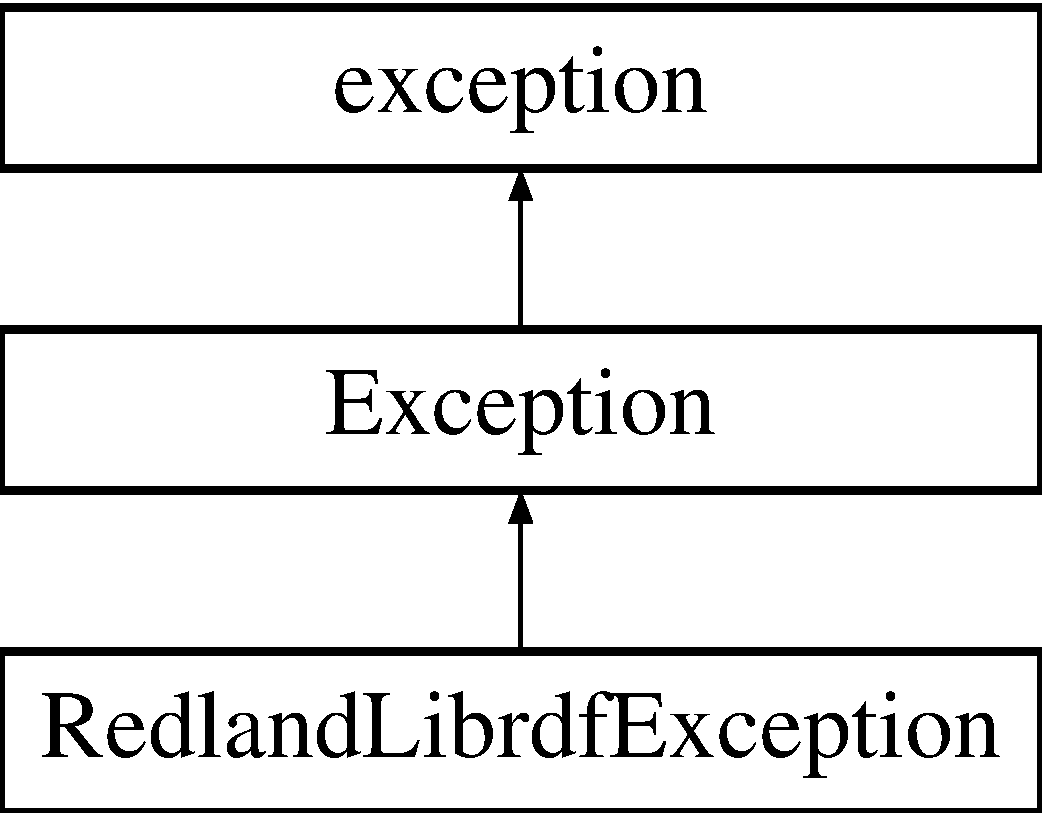
\includegraphics[height=3.000000cm]{classRedlandLibrdfException}
\end{center}
\end{figure}
\subsection*{Additional Inherited Members}


The documentation for this class was generated from the following file\+:\begin{DoxyCompactItemize}
\item 
src/redland/\+Redland\+A\+P\+I\+Wrapper/src/Librdf\+Exception.\+h\end{DoxyCompactItemize}

\hypertarget{classRedlandNullPointerException}{}\doxysection{Redland\+Null\+Pointer\+Exception Class Reference}
\label{classRedlandNullPointerException}\index{RedlandNullPointerException@{RedlandNullPointerException}}
Inheritance diagram for Redland\+Null\+Pointer\+Exception\+:\begin{figure}[H]
\begin{center}
\leavevmode
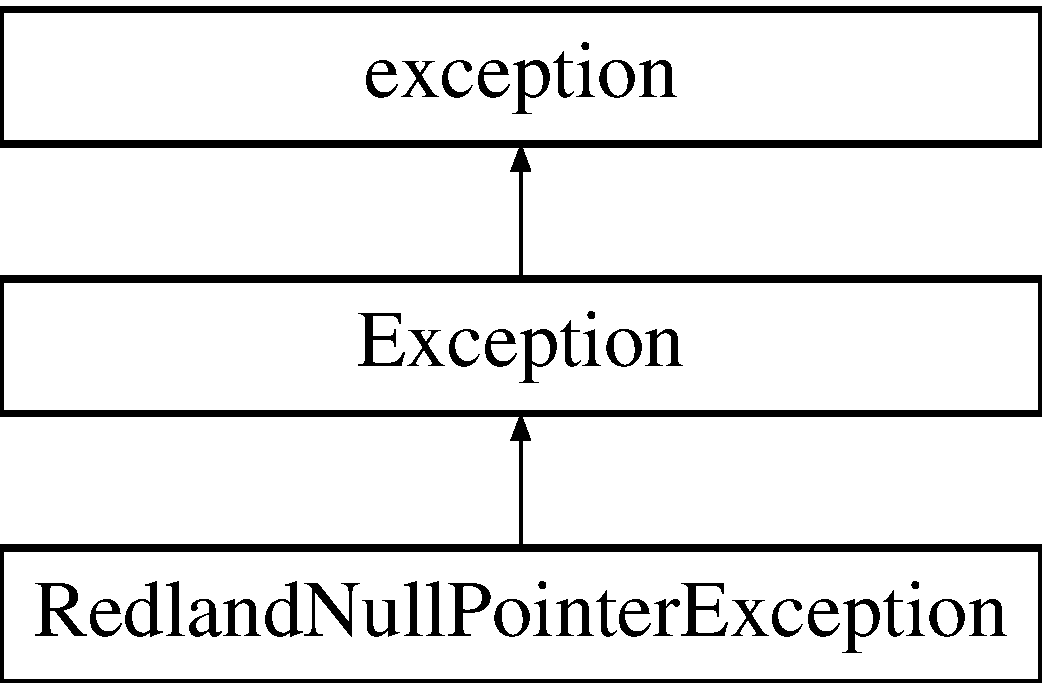
\includegraphics[height=3.000000cm]{classRedlandNullPointerException}
\end{center}
\end{figure}
\doxysubsection*{Additional Inherited Members}


The documentation for this class was generated from the following file\+:\begin{DoxyCompactItemize}
\item 
src/redland/\+Redland\+Wrapper/src/Librdf\+Exception.\+h\end{DoxyCompactItemize}

\hypertarget{classomexmeta_1_1Resource}{}\doxysection{omexmeta\+::Resource Class Reference}
\label{classomexmeta_1_1Resource}\index{omexmeta::Resource@{omexmeta::Resource}}
\doxysubsection*{Public Member Functions}
\begin{DoxyCompactItemize}
\item 
\mbox{\Hypertarget{classomexmeta_1_1Resource_ade5147df30b7e4f42386534a4a27b12f}\label{classomexmeta_1_1Resource_ade5147df30b7e4f42386534a4a27b12f}} 
bool {\bfseries operator==} (const \mbox{\hyperlink{classomexmeta_1_1Resource}{Resource}} \&rhs) const
\item 
\mbox{\Hypertarget{classomexmeta_1_1Resource_a99336c4dd6ef49588cd7144e50cf639b}\label{classomexmeta_1_1Resource_a99336c4dd6ef49588cd7144e50cf639b}} 
bool {\bfseries operator!=} (const \mbox{\hyperlink{classomexmeta_1_1Resource}{Resource}} \&rhs) const
\item 
\mbox{\Hypertarget{classomexmeta_1_1Resource_a6b70255d34f54c4adfa893a8ba54b0a2}\label{classomexmeta_1_1Resource_a6b70255d34f54c4adfa893a8ba54b0a2}} 
{\bfseries Resource} (\mbox{\hyperlink{classredland_1_1LibrdfNode}{Librdf\+Node}} node)
\item 
\mbox{\Hypertarget{classomexmeta_1_1Resource_a25be1a34d6a27565612a9c7b597befd8}\label{classomexmeta_1_1Resource_a25be1a34d6a27565612a9c7b597befd8}} 
void {\bfseries set\+Node} (\mbox{\hyperlink{structraptor__term}{librdf\+\_\+node}} $\ast$node)
\item 
\mbox{\Hypertarget{classomexmeta_1_1Resource_a7866b5bd47b319e39dec70eae8969d4f}\label{classomexmeta_1_1Resource_a7866b5bd47b319e39dec70eae8969d4f}} 
\mbox{\hyperlink{structraptor__term}{librdf\+\_\+node}} $\ast$ {\bfseries get\+Node} () const
\item 
\mbox{\Hypertarget{classomexmeta_1_1Resource_aae0948ff89d537133fd5e99bb88aa96a}\label{classomexmeta_1_1Resource_aae0948ff89d537133fd5e99bb88aa96a}} 
std\+::string {\bfseries str} () const
\item 
\mbox{\Hypertarget{classomexmeta_1_1Resource_ad6a1a5009a2b8fdacf0f53899986735a}\label{classomexmeta_1_1Resource_ad6a1a5009a2b8fdacf0f53899986735a}} 
virtual bool {\bfseries is\+Set} () const
\item 
\mbox{\Hypertarget{classomexmeta_1_1Resource_a87a7540d96d762dbd3f0b5160e575803}\label{classomexmeta_1_1Resource_a87a7540d96d762dbd3f0b5160e575803}} 
void {\bfseries free} ()
\end{DoxyCompactItemize}
\doxysubsection*{Static Public Member Functions}
\begin{DoxyCompactItemize}
\item 
\mbox{\Hypertarget{classomexmeta_1_1Resource_a4b8f2429e43312eab63b5135fd508986}\label{classomexmeta_1_1Resource_a4b8f2429e43312eab63b5135fd508986}} 
static \mbox{\hyperlink{classomexmeta_1_1Resource}{Resource}} {\bfseries from\+Raw\+Ptr} (\mbox{\hyperlink{structraptor__term}{librdf\+\_\+node}} $\ast$node)
\end{DoxyCompactItemize}
\doxysubsection*{Protected Attributes}
\begin{DoxyCompactItemize}
\item 
\mbox{\Hypertarget{classomexmeta_1_1Resource_a9695da843dd795e090f8b89886d432b9}\label{classomexmeta_1_1Resource_a9695da843dd795e090f8b89886d432b9}} 
\mbox{\hyperlink{structraptor__term}{librdf\+\_\+node}} $\ast$ {\bfseries node\+\_\+} = nullptr
\end{DoxyCompactItemize}


The documentation for this class was generated from the following files\+:\begin{DoxyCompactItemize}
\item 
src/omexmeta/include/omexmeta/Resource.\+h\item 
src/omexmeta/Resource.\+cpp\end{DoxyCompactItemize}

\hypertarget{classomexmeta_1_1SBMLAssistant}{}\section{omexmeta\+:\+:S\+B\+M\+L\+Assistant Class Reference}
\label{classomexmeta_1_1SBMLAssistant}\index{omexmeta\+::\+S\+B\+M\+L\+Assistant@{omexmeta\+::\+S\+B\+M\+L\+Assistant}}
Inheritance diagram for omexmeta\+:\+:S\+B\+M\+L\+Assistant\+:\begin{figure}[H]
\begin{center}
\leavevmode
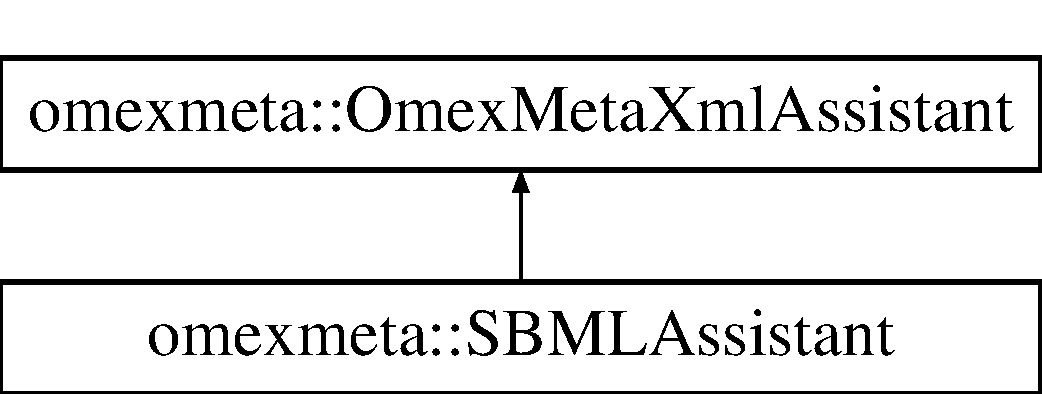
\includegraphics[height=2.000000cm]{classomexmeta_1_1SBMLAssistant}
\end{center}
\end{figure}
\subsection*{Public Member Functions}
\begin{DoxyCompactItemize}
\item 
\mbox{\Hypertarget{classomexmeta_1_1SBMLAssistant_afcc69d3e7a12673071632f757290d798}\label{classomexmeta_1_1SBMLAssistant_afcc69d3e7a12673071632f757290d798}} 
std\+::vector$<$ std\+::string $>$ {\bfseries get\+Valid\+Elements} () const override
\item 
\mbox{\Hypertarget{classomexmeta_1_1SBMLAssistant_ad3c3ab0ac3004961e5c2951568528d8a}\label{classomexmeta_1_1SBMLAssistant_ad3c3ab0ac3004961e5c2951568528d8a}} 
std\+::string {\bfseries meta\+Id\+Tag\+Name} () const override
\end{DoxyCompactItemize}


The documentation for this class was generated from the following files\+:\begin{DoxyCompactItemize}
\item 
src/omexmeta/Omex\+Meta\+Xml\+Assistant.\+h\item 
src/omexmeta/Omex\+Meta\+Xml\+Assistant.\+cpp\end{DoxyCompactItemize}

\hypertarget{classomexmeta_1_1SBMLSemanticExtraction}{}\section{omexmeta\+:\+:S\+B\+M\+L\+Semantic\+Extraction Class Reference}
\label{classomexmeta_1_1SBMLSemanticExtraction}\index{omexmeta\+::\+S\+B\+M\+L\+Semantic\+Extraction@{omexmeta\+::\+S\+B\+M\+L\+Semantic\+Extraction}}
\subsection*{Public Member Functions}
\begin{DoxyCompactItemize}
\item 
\mbox{\Hypertarget{classomexmeta_1_1SBMLSemanticExtraction_a3c55dab129bd47c753f19317fade1f18}\label{classomexmeta_1_1SBMLSemanticExtraction_a3c55dab129bd47c753f19317fade1f18}} 
{\bfseries S\+B\+M\+L\+Semantic\+Extraction} (\hyperlink{classomexmeta_1_1Editor}{Editor} $\ast$editor)
\item 
\mbox{\Hypertarget{classomexmeta_1_1SBMLSemanticExtraction_a53cda7f108b954af7fb1159773e44522}\label{classomexmeta_1_1SBMLSemanticExtraction_a53cda7f108b954af7fb1159773e44522}} 
void {\bfseries extract\+Species\+Compartment\+Semantics} ()
\item 
\mbox{\Hypertarget{classomexmeta_1_1SBMLSemanticExtraction_a89ed78df066e71e628c8b631175a8441}\label{classomexmeta_1_1SBMLSemanticExtraction_a89ed78df066e71e628c8b631175a8441}} 
void {\bfseries extract\+Processes\+From\+Reactions} ()
\end{DoxyCompactItemize}


The documentation for this class was generated from the following files\+:\begin{DoxyCompactItemize}
\item 
src/omexmeta/S\+B\+M\+L\+Semantic\+Extraction.\+h\item 
src/omexmeta/S\+B\+M\+L\+Semantic\+Extraction.\+cpp\end{DoxyCompactItemize}

\hypertarget{classomexmeta_1_1SemSim}{}\doxysection{omexmeta\+::Sem\+Sim Class Reference}
\label{classomexmeta_1_1SemSim}\index{omexmeta::SemSim@{omexmeta::SemSim}}
Inheritance diagram for omexmeta\+::Sem\+Sim\+:\begin{figure}[H]
\begin{center}
\leavevmode
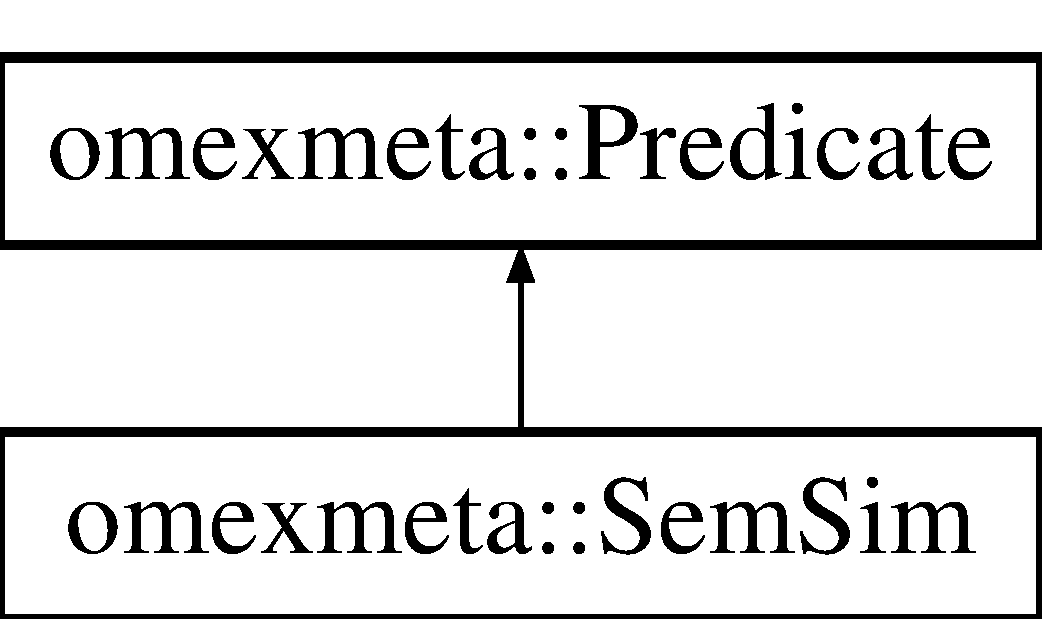
\includegraphics[height=2.000000cm]{classomexmeta_1_1SemSim}
\end{center}
\end{figure}
\doxysubsection*{Public Member Functions}
\begin{DoxyCompactItemize}
\item 
\mbox{\Hypertarget{classomexmeta_1_1SemSim_a957a762d9f721bfc74f0db91552068a4}\label{classomexmeta_1_1SemSim_a957a762d9f721bfc74f0db91552068a4}} 
{\bfseries Sem\+Sim} (const std\+::string \&term)
\item 
\mbox{\Hypertarget{classomexmeta_1_1SemSim_a40dcb1f6945bba21cc6927cf78a53e80}\label{classomexmeta_1_1SemSim_a40dcb1f6945bba21cc6927cf78a53e80}} 
void {\bfseries verify} ()
\end{DoxyCompactItemize}
\doxysubsection*{Public Attributes}
\begin{DoxyCompactItemize}
\item 
std\+::vector$<$ std\+::string $>$ {\bfseries valid\+\_\+terms\+\_\+}
\end{DoxyCompactItemize}
\doxysubsection*{Additional Inherited Members}


\doxysubsection{Member Data Documentation}
\mbox{\Hypertarget{classomexmeta_1_1SemSim_af6e027f353354892e3a26abb9b6f2ece}\label{classomexmeta_1_1SemSim_af6e027f353354892e3a26abb9b6f2ece}} 
\index{omexmeta::SemSim@{omexmeta::SemSim}!valid\_terms\_@{valid\_terms\_}}
\index{valid\_terms\_@{valid\_terms\_}!omexmeta::SemSim@{omexmeta::SemSim}}
\doxysubsubsection{\texorpdfstring{valid\_terms\_}{valid\_terms\_}}
{\footnotesize\ttfamily std\+::vector$<$std\+::string$>$ omexmeta\+::\+Sem\+Sim\+::valid\+\_\+terms\+\_\+}

{\bfseries Initial value\+:}
\begin{DoxyCode}{0}
\DoxyCodeLine{\{}
\DoxyCodeLine{                \textcolor{stringliteral}{"{}hasSourceParticipant"{}},}
\DoxyCodeLine{                \textcolor{stringliteral}{"{}hasSinkParticipant"{}},}
\DoxyCodeLine{                \textcolor{stringliteral}{"{}hasMediatorParticipant"{}},}
\DoxyCodeLine{                \textcolor{stringliteral}{"{}hasMultiplier"{}},}
\DoxyCodeLine{                \textcolor{stringliteral}{"{}hasPhysicalEntityReference"{}},}
\DoxyCodeLine{        \}}

\end{DoxyCode}


The documentation for this class was generated from the following files\+:\begin{DoxyCompactItemize}
\item 
src/omexmeta/Predicate.\+h\item 
src/omexmeta/Predicate.\+cpp\end{DoxyCompactItemize}

\hypertarget{classomexmeta_1_1SemsimXmlAssistantFactory}{}\doxysection{omexmeta\+::Semsim\+Xml\+Assistant\+Factory Class Reference}
\label{classomexmeta_1_1SemsimXmlAssistantFactory}\index{omexmeta::SemsimXmlAssistantFactory@{omexmeta::SemsimXmlAssistantFactory}}
\doxysubsection*{Static Public Member Functions}
\begin{DoxyCompactItemize}
\item 
\mbox{\Hypertarget{classomexmeta_1_1SemsimXmlAssistantFactory_acd1e70258ce2a70ff459f9ff905c2371}\label{classomexmeta_1_1SemsimXmlAssistantFactory_acd1e70258ce2a70ff459f9ff905c2371}} 
static Xml\+Assistant\+Ptr {\bfseries generate} (const std\+::string \&xml, Omex\+Meta\+Xml\+Type type, bool generate\+\_\+new\+\_\+metaids=false, std\+::string metaid\+\_\+base=\char`\"{}\#Omex\+Meta\+Id\char`\"{}, int metaid\+\_\+num\+\_\+digits=4)
\end{DoxyCompactItemize}


The documentation for this class was generated from the following files\+:\begin{DoxyCompactItemize}
\item 
src/omexmeta/Omex\+Meta\+Xml\+Assistant.\+h\item 
src/omexmeta/Omex\+Meta\+Xml\+Assistant.\+cpp\end{DoxyCompactItemize}

\hypertarget{classomexmeta_1_1SinkParticipant}{}\doxysection{omexmeta\+::Sink\+Participant Class Reference}
\label{classomexmeta_1_1SinkParticipant}\index{omexmeta::SinkParticipant@{omexmeta::SinkParticipant}}


{\ttfamily \#include $<$Participant.\+h$>$}

Inheritance diagram for omexmeta\+::Sink\+Participant\+:\begin{figure}[H]
\begin{center}
\leavevmode
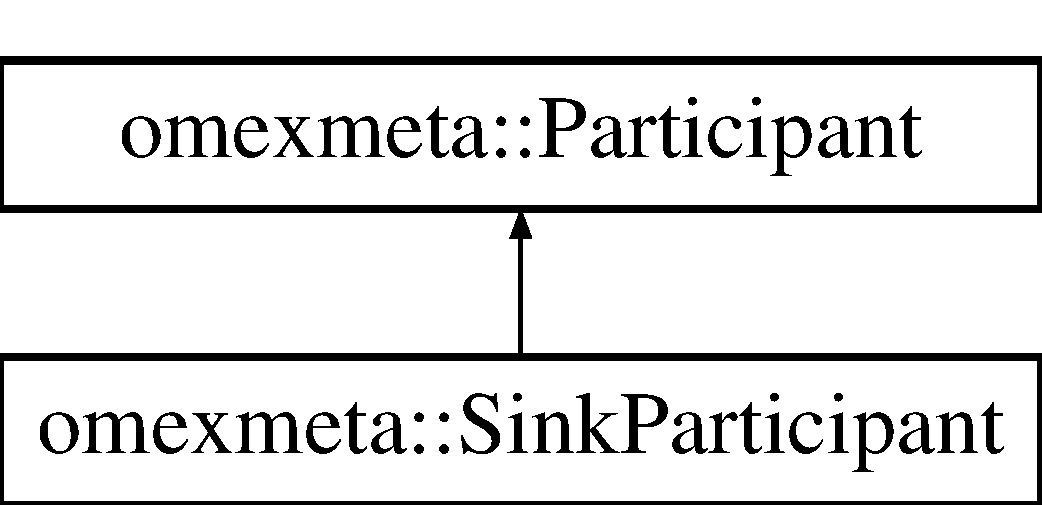
\includegraphics[height=2.000000cm]{classomexmeta_1_1SinkParticipant}
\end{center}
\end{figure}
\doxysubsection*{Public Member Functions}
\begin{DoxyCompactItemize}
\item 
\mbox{\Hypertarget{classomexmeta_1_1SinkParticipant_a080d3b3379b4dfb24ea8bbb8186df4d1}\label{classomexmeta_1_1SinkParticipant_a080d3b3379b4dfb24ea8bbb8186df4d1}} 
\mbox{\hyperlink{classomexmeta_1_1SinkParticipant_a080d3b3379b4dfb24ea8bbb8186df4d1}{Sink\+Participant}} (\mbox{\hyperlink{classredland_1_1LibrdfModel}{Librdf\+Model}} \&model, double multiplier, std\+::string physical\+Entity\+Reference, e\+Uri\+Type type, \mbox{\hyperlink{classomexmeta_1_1UriHandler}{Uri\+Handler}} \&uri\+Handler)
\begin{DoxyCompactList}\small\item\em A class representing process/force energetic sinks. \end{DoxyCompactList}\end{DoxyCompactItemize}


\doxysubsection{Detailed Description}
\mbox{\hyperlink{classSubclass}{Subclass}} of \mbox{\hyperlink{classomexmeta_1_1Participant}{Participant}}. See Participants for arguments. 

The documentation for this class was generated from the following files\+:\begin{DoxyCompactItemize}
\item 
src/omexmeta/include/omexmeta/Participant.\+h\item 
src/omexmeta/Participant.\+cpp\end{DoxyCompactItemize}

\hypertarget{classomexmeta_1_1SourceParticipant}{}\section{omexmeta\+:\+:Source\+Participant Class Reference}
\label{classomexmeta_1_1SourceParticipant}\index{omexmeta\+::\+Source\+Participant@{omexmeta\+::\+Source\+Participant}}
Inheritance diagram for omexmeta\+:\+:Source\+Participant\+:\begin{figure}[H]
\begin{center}
\leavevmode
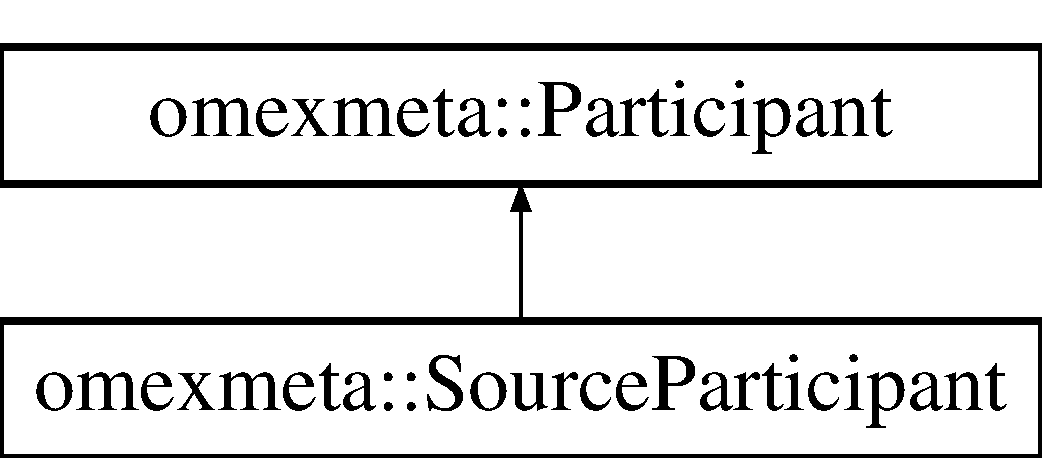
\includegraphics[height=2.000000cm]{classomexmeta_1_1SourceParticipant}
\end{center}
\end{figure}
\subsection*{Public Member Functions}
\begin{DoxyCompactItemize}
\item 
\mbox{\Hypertarget{classomexmeta_1_1SourceParticipant_a84b77b854e235cc9e0cb8da2b6a2cee5}\label{classomexmeta_1_1SourceParticipant_a84b77b854e235cc9e0cb8da2b6a2cee5}} 
{\bfseries Source\+Participant} (librdf\+\_\+model $\ast$model, int multiplier, std\+::string physical\+Entity\+Reference, const std\+::string \&model\+\_\+uri, const std\+::string \&local\+\_\+uri)
\end{DoxyCompactItemize}


The documentation for this class was generated from the following files\+:\begin{DoxyCompactItemize}
\item 
src/omexmeta/Participant.\+h\item 
src/omexmeta/Participant.\+cpp\end{DoxyCompactItemize}

\hypertarget{classomexmeta_1_1Subject}{}\doxysection{omexmeta\+::Subject Class Reference}
\label{classomexmeta_1_1Subject}\index{omexmeta::Subject@{omexmeta::Subject}}
\doxysubsection*{Public Member Functions}
\begin{DoxyCompactItemize}
\item 
\mbox{\Hypertarget{classomexmeta_1_1Subject_a4e80ab7745a8c2cf6628e8e93a95cdac}\label{classomexmeta_1_1Subject_a4e80ab7745a8c2cf6628e8e93a95cdac}} 
{\bfseries Subject} (\mbox{\hyperlink{classredland_1_1LibrdfNode}{Librdf\+Node}} node)
\item 
\mbox{\Hypertarget{classomexmeta_1_1Subject_a91ea148978a5320dfba19bdb1bdbdd90}\label{classomexmeta_1_1Subject_a91ea148978a5320dfba19bdb1bdbdd90}} 
\mbox{\hyperlink{structraptor__term}{librdf\+\_\+node}} $\ast$ {\bfseries get\+Node} () const
\item 
\mbox{\Hypertarget{classomexmeta_1_1Subject_aa04b4e973bd7df44fffe588e31b8779f}\label{classomexmeta_1_1Subject_aa04b4e973bd7df44fffe588e31b8779f}} 
void {\bfseries set\+Node} (\mbox{\hyperlink{structraptor__term}{librdf\+\_\+node}} $\ast$node)
\item 
\mbox{\Hypertarget{classomexmeta_1_1Subject_a1b170dceee7bf297843da5b201e06693}\label{classomexmeta_1_1Subject_a1b170dceee7bf297843da5b201e06693}} 
bool {\bfseries operator==} (const \mbox{\hyperlink{classomexmeta_1_1Subject}{Subject}} \&rhs) const
\item 
\mbox{\Hypertarget{classomexmeta_1_1Subject_a3729c201061ff27fc50b1ae2412dab2b}\label{classomexmeta_1_1Subject_a3729c201061ff27fc50b1ae2412dab2b}} 
bool {\bfseries operator!=} (const \mbox{\hyperlink{classomexmeta_1_1Subject}{Subject}} \&rhs) const
\item 
\mbox{\Hypertarget{classomexmeta_1_1Subject_a3aa59bfd78d3c6e138beb386d846a584}\label{classomexmeta_1_1Subject_a3aa59bfd78d3c6e138beb386d846a584}} 
std\+::string {\bfseries str} () const
\item 
\mbox{\Hypertarget{classomexmeta_1_1Subject_a1b4c539f6310fc0c834cc44afb275c32}\label{classomexmeta_1_1Subject_a1b4c539f6310fc0c834cc44afb275c32}} 
bool {\bfseries is\+Set} () const
\item 
\mbox{\Hypertarget{classomexmeta_1_1Subject_ac21da4aad49780ba33322de5b7f87756}\label{classomexmeta_1_1Subject_ac21da4aad49780ba33322de5b7f87756}} 
void {\bfseries free} ()
\end{DoxyCompactItemize}
\doxysubsection*{Static Public Member Functions}
\begin{DoxyCompactItemize}
\item 
\mbox{\Hypertarget{classomexmeta_1_1Subject_a845dda888ce07265306d0eb6b46cd989}\label{classomexmeta_1_1Subject_a845dda888ce07265306d0eb6b46cd989}} 
static \mbox{\hyperlink{classomexmeta_1_1Subject}{Subject}} {\bfseries from\+Raw\+Ptr} (\mbox{\hyperlink{structraptor__term}{librdf\+\_\+node}} $\ast$node)
\item 
\mbox{\Hypertarget{classomexmeta_1_1Subject_a346583235b81d5bd523818de09d7359e}\label{classomexmeta_1_1Subject_a346583235b81d5bd523818de09d7359e}} 
static \mbox{\hyperlink{classomexmeta_1_1Subject}{Subject}} {\bfseries from\+Uri} (const std\+::string \&uri)
\item 
\mbox{\Hypertarget{classomexmeta_1_1Subject_a315d058097112f4081c4db7860346aef}\label{classomexmeta_1_1Subject_a315d058097112f4081c4db7860346aef}} 
static \mbox{\hyperlink{classomexmeta_1_1Subject}{Subject}} {\bfseries from\+Blank} (const std\+::string \&blank)
\end{DoxyCompactItemize}


The documentation for this class was generated from the following files\+:\begin{DoxyCompactItemize}
\item 
src/omexmeta/include/omexmeta/Subject.\+h\item 
src/omexmeta/Subject.\+cpp\end{DoxyCompactItemize}

\hypertarget{structdbg_1_1time}{}\doxysection{dbg\+::time Struct Reference}
\label{structdbg_1_1time}\index{dbg::time@{dbg::time}}


The documentation for this struct was generated from the following file\+:\begin{DoxyCompactItemize}
\item 
src/omexmeta/dbg.\+h\end{DoxyCompactItemize}

\hypertarget{classomexmeta_1_1Triple}{}\doxysection{omexmeta\+::Triple Class Reference}
\label{classomexmeta_1_1Triple}\index{omexmeta::Triple@{omexmeta::Triple}}
Inheritance diagram for omexmeta\+::Triple\+:\begin{figure}[H]
\begin{center}
\leavevmode
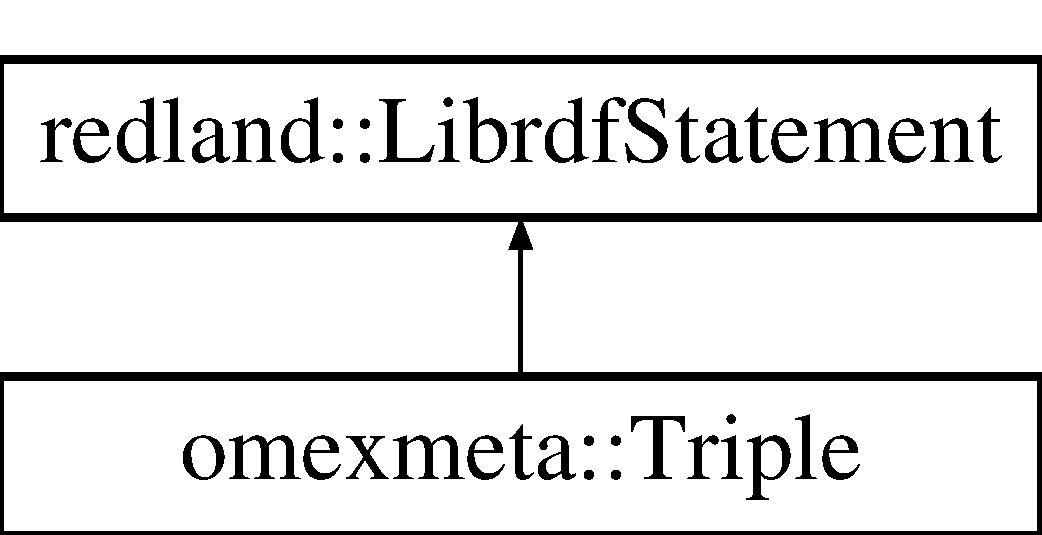
\includegraphics[height=2.000000cm]{classomexmeta_1_1Triple}
\end{center}
\end{figure}
\doxysubsection*{Public Member Functions}
\begin{DoxyCompactItemize}
\item 
\mbox{\Hypertarget{classomexmeta_1_1Triple_aaed857f9356dc3a7414f06f393a75ba0}\label{classomexmeta_1_1Triple_aaed857f9356dc3a7414f06f393a75ba0}} 
{\bfseries Triple} (const \mbox{\hyperlink{classomexmeta_1_1Subject}{Subject}} \&subject, const Predicate\+Ptr \&predicate\+\_\+ptr, const \mbox{\hyperlink{classomexmeta_1_1Resource}{Resource}} \&resource)
\item 
\mbox{\Hypertarget{classomexmeta_1_1Triple_adc457c78ec059eb71602e7ea4f763582}\label{classomexmeta_1_1Triple_adc457c78ec059eb71602e7ea4f763582}} 
{\bfseries Triple} (librdf\+\_\+node $\ast$subject, librdf\+\_\+node $\ast$predicate, librdf\+\_\+node $\ast$resource)
\item 
\mbox{\Hypertarget{classomexmeta_1_1Triple_a1cb45dd3a5778f0e0e92e4a185da9400}\label{classomexmeta_1_1Triple_a1cb45dd3a5778f0e0e92e4a185da9400}} 
const std\+::string \& {\bfseries get\+Local\+Uri} () const
\item 
\mbox{\Hypertarget{classomexmeta_1_1Triple_a6694daa46597ea91dda045aa0d5e6cfc}\label{classomexmeta_1_1Triple_a6694daa46597ea91dda045aa0d5e6cfc}} 
void \mbox{\hyperlink{classomexmeta_1_1Triple_a6694daa46597ea91dda045aa0d5e6cfc}{set\+Local\+Uri}} (std\+::string local\+Uri)
\begin{DoxyCompactList}\small\item\em set the local\+\_\+uri\+\_\+ attribute for this triple \end{DoxyCompactList}\item 
\mbox{\Hypertarget{classomexmeta_1_1Triple_afd918ecccfa23079d9cb70f2e1a3e9b0}\label{classomexmeta_1_1Triple_afd918ecccfa23079d9cb70f2e1a3e9b0}} 
void \mbox{\hyperlink{classomexmeta_1_1Triple_afd918ecccfa23079d9cb70f2e1a3e9b0}{set\+Model\+Uri}} (const std\+::string \&model\+\_\+uri)
\begin{DoxyCompactList}\small\item\em set the model\+\_\+uri\+\_\+ attribute for this triple \end{DoxyCompactList}\item 
std\+::string \mbox{\hyperlink{classomexmeta_1_1Triple_aabfef726172656b6c61c602b4d8d33e5}{str}} (const std\+::string \&format=\char`\"{}turtle\char`\"{}, const std\+::string \&base=(std\+::filesystem\+::current\+\_\+path()/=\char`\"{}annotations.\+rdf\char`\"{}).string(), std\+::string omex\+\_\+name=\char`\"{}New\+Omex.\+omex/\char`\"{}, std\+::string model\+\_\+name=\char`\"{}New\+Model.\+xml\#\char`\"{}) const
\begin{DoxyCompactList}\small\item\em serialize the triple using a @format serializer. \end{DoxyCompactList}\item 
\mbox{\Hypertarget{classomexmeta_1_1Triple_a3f3868622349d3a3e14ed3e4b21d49a9}\label{classomexmeta_1_1Triple_a3f3868622349d3a3e14ed3e4b21d49a9}} 
void {\bfseries free\+Triple} ()
\item 
\mbox{\Hypertarget{classomexmeta_1_1Triple_a2b673a8166a19fb4feae0fc42d31c105}\label{classomexmeta_1_1Triple_a2b673a8166a19fb4feae0fc42d31c105}} 
\mbox{\hyperlink{classomexmeta_1_1Triple}{Triple}} \& {\bfseries set\+About} (std\+::string omex\+\_\+name, const std\+::string \&model\+\_\+name, std\+::string metaid)
\item 
\mbox{\Hypertarget{classomexmeta_1_1Triple_a6329b09efb05005d248790e8a3d507f3}\label{classomexmeta_1_1Triple_a6329b09efb05005d248790e8a3d507f3}} 
\mbox{\hyperlink{classomexmeta_1_1Triple}{Triple}} \& {\bfseries set\+About} (std\+::string metaid)
\item 
\mbox{\Hypertarget{classomexmeta_1_1Triple_a69df88d19e2f9077fccfa9543dadd15f}\label{classomexmeta_1_1Triple_a69df88d19e2f9077fccfa9543dadd15f}} 
std\+::string {\bfseries get\+About} () const
\item 
\mbox{\Hypertarget{classomexmeta_1_1Triple_a886240fe50becaaa47ca171f2d454ba4}\label{classomexmeta_1_1Triple_a886240fe50becaaa47ca171f2d454ba4}} 
librdf\+\_\+statement $\ast$ {\bfseries get\+Statement} () const
\item 
\mbox{\Hypertarget{classomexmeta_1_1Triple_a57b4521321178af38415e76cd483207e}\label{classomexmeta_1_1Triple_a57b4521321178af38415e76cd483207e}} 
\mbox{\hyperlink{classomexmeta_1_1Triple}{Triple}} \& {\bfseries set\+Predicate} (const std\+::string \&namespace\+\_\+, const std\+::string \&term)
\item 
\mbox{\Hypertarget{classomexmeta_1_1Triple_a7358812badc8d0d5589a0165af4ad375}\label{classomexmeta_1_1Triple_a7358812badc8d0d5589a0165af4ad375}} 
\mbox{\hyperlink{classomexmeta_1_1Triple}{Triple}} \& {\bfseries set\+Resource\+Literal} (const std\+::string \&literal)
\item 
\mbox{\Hypertarget{classomexmeta_1_1Triple_ae6836c6e9d06a310a120345aa95a4daa}\label{classomexmeta_1_1Triple_ae6836c6e9d06a310a120345aa95a4daa}} 
\mbox{\hyperlink{classomexmeta_1_1Triple}{Triple}} \& {\bfseries set\+Resource\+Uri} (const std\+::string \&identifiers\+\_\+uri)
\item 
\mbox{\Hypertarget{classomexmeta_1_1Triple_a90ffe9b74d354cc3fe3132a07546f6d1}\label{classomexmeta_1_1Triple_a90ffe9b74d354cc3fe3132a07546f6d1}} 
\mbox{\hyperlink{classomexmeta_1_1Triple}{Triple}} \& {\bfseries set\+Resource\+Blank} (const std\+::string \&blank\+\_\+id)
\item 
\mbox{\Hypertarget{classomexmeta_1_1Triple_a34832780748d58b0fddea6f6f079217a}\label{classomexmeta_1_1Triple_a34832780748d58b0fddea6f6f079217a}} 
bool {\bfseries is\+Empty} ()
\item 
\mbox{\Hypertarget{classomexmeta_1_1Triple_a1a99a566a9d1883c6329a023f4dbc056}\label{classomexmeta_1_1Triple_a1a99a566a9d1883c6329a023f4dbc056}} 
\mbox{\hyperlink{classomexmeta_1_1Triple}{Triple}} \& {\bfseries set\+Predicate} (const std\+::string \&uri)
\item 
\mbox{\Hypertarget{classomexmeta_1_1Triple_ab89993902b551b98d9e17e4fe5ebed6b}\label{classomexmeta_1_1Triple_ab89993902b551b98d9e17e4fe5ebed6b}} 
void {\bfseries free\+Triple\+And\+Uris} ()
\item 
\mbox{\Hypertarget{classomexmeta_1_1Triple_ac379e5410a41c1946e91d581f023c7f5}\label{classomexmeta_1_1Triple_ac379e5410a41c1946e91d581f023c7f5}} 
const std\+::string \& {\bfseries get\+Model\+Uri} () const
\item 
\mbox{\Hypertarget{classomexmeta_1_1Triple_a44d31389b0056ab4f1d8689521a25032}\label{classomexmeta_1_1Triple_a44d31389b0056ab4f1d8689521a25032}} 
\mbox{\hyperlink{classomexmeta_1_1Triple}{Triple}} \& {\bfseries set\+Resource\+With\+Model\+Uri} (const std\+::string \&metaid)
\end{DoxyCompactItemize}
\doxysubsection*{Static Public Member Functions}
\begin{DoxyCompactItemize}
\item 
\mbox{\Hypertarget{classomexmeta_1_1Triple_af03c0ce3392c0ff30f13772209ac873c}\label{classomexmeta_1_1Triple_af03c0ce3392c0ff30f13772209ac873c}} 
static \mbox{\hyperlink{classomexmeta_1_1Triple}{Triple}} {\bfseries from\+Raw\+Statement\+Ptr} (librdf\+\_\+statement $\ast$statement)
\end{DoxyCompactItemize}
\doxysubsection*{Additional Inherited Members}


\doxysubsection{Member Function Documentation}
\mbox{\Hypertarget{classomexmeta_1_1Triple_aabfef726172656b6c61c602b4d8d33e5}\label{classomexmeta_1_1Triple_aabfef726172656b6c61c602b4d8d33e5}} 
\index{omexmeta::Triple@{omexmeta::Triple}!str@{str}}
\index{str@{str}!omexmeta::Triple@{omexmeta::Triple}}
\doxysubsubsection{\texorpdfstring{str()}{str()}}
{\footnotesize\ttfamily std\+::string omexmeta\+::\+Triple\+::str (\begin{DoxyParamCaption}\item[{const std\+::string \&}]{format = {\ttfamily \char`\"{}turtle\char`\"{}},  }\item[{const std\+::string \&}]{base = {\ttfamily (std\+:\+:filesystem\+:\+:current\+\_\+path()~/=~~\char`\"{}annotations.rdf\char`\"{}).string()},  }\item[{std\+::string}]{omex\+\_\+name = {\ttfamily \char`\"{}NewOmex.omex/\char`\"{}},  }\item[{std\+::string}]{model\+\_\+name = {\ttfamily \char`\"{}NewModel.xml\#\char`\"{}} }\end{DoxyParamCaption}) const}



serialize the triple using a @format serializer. 

\begin{DoxyVerb}Creates an isolated serializer that does not get added
to the users annotations. This method is for visualizing
a triple only.
\end{DoxyVerb}
 

The documentation for this class was generated from the following files\+:\begin{DoxyCompactItemize}
\item 
src/omexmeta/Triple.\+h\item 
src/omexmeta/Triple.\+cpp\end{DoxyCompactItemize}

\hypertarget{classomexmeta_1_1Triples}{}\section{omexmeta\+:\+:Triples Class Reference}
\label{classomexmeta_1_1Triples}\index{omexmeta\+::\+Triples@{omexmeta\+::\+Triples}}
\subsection*{Public Member Functions}
\begin{DoxyCompactItemize}
\item 
\mbox{\Hypertarget{classomexmeta_1_1Triples_a32ea34c1fd3bfe9887c2221377392efe}\label{classomexmeta_1_1Triples_a32ea34c1fd3bfe9887c2221377392efe}} 
{\bfseries Triples} (int size)
\item 
\mbox{\Hypertarget{classomexmeta_1_1Triples_a733eea0f6a2c206eb96771bc7a8cb430}\label{classomexmeta_1_1Triples_a733eea0f6a2c206eb96771bc7a8cb430}} 
{\bfseries Triples} (\hyperlink{classomexmeta_1_1Triple}{Triple} \&triple)
\item 
\mbox{\Hypertarget{classomexmeta_1_1Triples_a71a3ff7b185a5420eabd9bf4e9637196}\label{classomexmeta_1_1Triples_a71a3ff7b185a5420eabd9bf4e9637196}} 
{\bfseries Triples} (std\+::vector$<$ \hyperlink{classomexmeta_1_1Triple}{Triple} $>$ triples)
\item 
\mbox{\Hypertarget{classomexmeta_1_1Triples_a8c6e00fe9e694d9c52e1fa37a82ae489}\label{classomexmeta_1_1Triples_a8c6e00fe9e694d9c52e1fa37a82ae489}} 
bool {\bfseries operator==} (const \hyperlink{classomexmeta_1_1Triples}{Triples} \&rhs) const
\item 
\mbox{\Hypertarget{classomexmeta_1_1Triples_a8c9df0d37572179d682127cb7368dd82}\label{classomexmeta_1_1Triples_a8c9df0d37572179d682127cb7368dd82}} 
bool {\bfseries operator!=} (const \hyperlink{classomexmeta_1_1Triples}{Triples} \&rhs) const
\item 
\mbox{\Hypertarget{classomexmeta_1_1Triples_a88dcf4b950f105acb621bd07f07a38a0}\label{classomexmeta_1_1Triples_a88dcf4b950f105acb621bd07f07a38a0}} 
void {\bfseries move\+\_\+back} (\hyperlink{classomexmeta_1_1Triple}{Triple} \&triple)
\item 
\mbox{\Hypertarget{classomexmeta_1_1Triples_a9882f6f582e8d2e34e09d2f7076a0e2e}\label{classomexmeta_1_1Triples_a9882f6f582e8d2e34e09d2f7076a0e2e}} 
void {\bfseries emplace\+\_\+back} (\hyperlink{classomexmeta_1_1Subject}{Subject} subject, const Predicate\+Ptr \&predicate\+Ptr, const \hyperlink{classomexmeta_1_1Resource}{Resource} \&resource)
\item 
\mbox{\Hypertarget{classomexmeta_1_1Triples_acab4513889a9a42c77b3044aac941728}\label{classomexmeta_1_1Triples_acab4513889a9a42c77b3044aac941728}} 
void {\bfseries emplace\+\_\+back} (\hyperlink{classomexmeta_1_1Subject}{Subject} subject, const \hyperlink{classomexmeta_1_1Predicate}{Predicate} \&predicate, const \hyperlink{classomexmeta_1_1Resource}{Resource} \&resource)
\item 
\mbox{\Hypertarget{classomexmeta_1_1Triples_a862d672c0ac9d877261947cf5a7061db}\label{classomexmeta_1_1Triples_a862d672c0ac9d877261947cf5a7061db}} 
void {\bfseries emplace\+\_\+back} (\hyperlink{classomexmeta_1_1Subject}{Subject} subject, \hyperlink{classomexmeta_1_1BiomodelsBiologyQualifier}{Biomodels\+Biology\+Qualifier} predicate, const \hyperlink{classomexmeta_1_1Resource}{Resource} \&resource)
\item 
\mbox{\Hypertarget{classomexmeta_1_1Triples_a87cdc3aacef07c2aebbfe06342bd70f5}\label{classomexmeta_1_1Triples_a87cdc3aacef07c2aebbfe06342bd70f5}} 
void {\bfseries emplace\+\_\+back} (\hyperlink{classomexmeta_1_1Subject}{Subject} subject, \hyperlink{classomexmeta_1_1BiomodelsModelQualifier}{Biomodels\+Model\+Qualifier} predicate, const \hyperlink{classomexmeta_1_1Resource}{Resource} \&resource)
\item 
\mbox{\Hypertarget{classomexmeta_1_1Triples_a9f3f3152592f99ac95f65e0e7ce3b450}\label{classomexmeta_1_1Triples_a9f3f3152592f99ac95f65e0e7ce3b450}} 
void {\bfseries emplace\+\_\+back} (\hyperlink{classomexmeta_1_1Subject}{Subject} subject, \hyperlink{classomexmeta_1_1DCTerm}{D\+C\+Term} predicate, const \hyperlink{classomexmeta_1_1Resource}{Resource} \&resource)
\item 
\mbox{\Hypertarget{classomexmeta_1_1Triples_a55e7ed1c3212ae19d2189a386b81422e}\label{classomexmeta_1_1Triples_a55e7ed1c3212ae19d2189a386b81422e}} 
void {\bfseries emplace\+\_\+back} (\hyperlink{classomexmeta_1_1Subject}{Subject} subject, \hyperlink{classomexmeta_1_1SemSim}{Sem\+Sim} predicate, const \hyperlink{classomexmeta_1_1Resource}{Resource} \&resource)
\item 
\mbox{\Hypertarget{classomexmeta_1_1Triples_a3a8c150cff4d1e78aa360d62d3d6604e}\label{classomexmeta_1_1Triples_a3a8c150cff4d1e78aa360d62d3d6604e}} 
void {\bfseries emplace\+\_\+back} (librdf\+\_\+node $\ast$subject, librdf\+\_\+node $\ast$predicate, librdf\+\_\+node $\ast$resource)
\item 
\mbox{\Hypertarget{classomexmeta_1_1Triples_a5234882414a2aaaca603eacd805df3d6}\label{classomexmeta_1_1Triples_a5234882414a2aaaca603eacd805df3d6}} 
std\+::vector$<$ std\+::string $>$ {\bfseries get\+Subjects\+Str} ()
\item 
\mbox{\Hypertarget{classomexmeta_1_1Triples_a63639c08caac19e6c5cbf30bb28292d0}\label{classomexmeta_1_1Triples_a63639c08caac19e6c5cbf30bb28292d0}} 
std\+::vector$<$ std\+::string $>$ {\bfseries get\+Predicates} ()
\item 
\mbox{\Hypertarget{classomexmeta_1_1Triples_aa875120a73cb1618be9e699e8bfb08c4}\label{classomexmeta_1_1Triples_aa875120a73cb1618be9e699e8bfb08c4}} 
std\+::vector$<$ std\+::string $>$ {\bfseries get\+Resources} ()
\item 
\mbox{\Hypertarget{classomexmeta_1_1Triples_adc86427b3563d04849336a8da7566451}\label{classomexmeta_1_1Triples_adc86427b3563d04849336a8da7566451}} 
int {\bfseries size} () const
\item 
\mbox{\Hypertarget{classomexmeta_1_1Triples_aa6735eb506ff0d5a3179fab3af3b2602}\label{classomexmeta_1_1Triples_aa6735eb506ff0d5a3179fab3af3b2602}} 
Triple\+Vector\+::iterator {\bfseries begin} ()
\item 
\mbox{\Hypertarget{classomexmeta_1_1Triples_a4312337b242280bcb119908c0334bfd8}\label{classomexmeta_1_1Triples_a4312337b242280bcb119908c0334bfd8}} 
Triple\+Vector\+::iterator {\bfseries end} ()
\item 
\mbox{\Hypertarget{classomexmeta_1_1Triples_a62d145b37f9d1e4b48b2164b8c6c0990}\label{classomexmeta_1_1Triples_a62d145b37f9d1e4b48b2164b8c6c0990}} 
std\+::string {\bfseries str} (const std\+::string \&format=\char`\"{}rdfxml-\/abbrev\char`\"{}, std\+::string base=(std\+::filesystem\+::current\+\_\+path()/=\char`\"{}annotations.\+rdf\char`\"{}).string(), std\+::string omex\+\_\+name=\char`\"{}New\+Omex.\+omex\char`\"{}, std\+::string model\+\_\+name=\char`\"{}New\+Model.\+xml\#\char`\"{})
\item 
\mbox{\Hypertarget{classomexmeta_1_1Triples_ad0c5839b0f49d6427cf53004baf9b0f4}\label{classomexmeta_1_1Triples_ad0c5839b0f49d6427cf53004baf9b0f4}} 
void {\bfseries free\+Triples} ()
\item 
\mbox{\Hypertarget{classomexmeta_1_1Triples_a5dad8f2cde0a3f6c0ce341338f80b0cd}\label{classomexmeta_1_1Triples_a5dad8f2cde0a3f6c0ce341338f80b0cd}} 
\hyperlink{classomexmeta_1_1Triple}{Triple} {\bfseries pop} ()
\item 
\mbox{\Hypertarget{classomexmeta_1_1Triples_a43d540423a436986d9f72d7cf0f02d72}\label{classomexmeta_1_1Triples_a43d540423a436986d9f72d7cf0f02d72}} 
const \hyperlink{classomexmeta_1_1Triple}{Triple} \& {\bfseries operator\mbox{[}$\,$\mbox{]}} (int index) const
\item 
\mbox{\Hypertarget{classomexmeta_1_1Triples_a48ab93d0e38e3cfcb4eac9264b047f0a}\label{classomexmeta_1_1Triples_a48ab93d0e38e3cfcb4eac9264b047f0a}} 
bool {\bfseries is\+Empty} ()
\item 
\mbox{\Hypertarget{classomexmeta_1_1Triples_abb333b83c7a8ed1f210816ef88c8d3a0}\label{classomexmeta_1_1Triples_abb333b83c7a8ed1f210816ef88c8d3a0}} 
\hyperlink{classomexmeta_1_1Triple}{Triple} {\bfseries pop\+\_\+front} ()
\item 
\mbox{\Hypertarget{classomexmeta_1_1Triples_a1f7ba9d5cd575ba5c63ed9dbbd1f279c}\label{classomexmeta_1_1Triples_a1f7ba9d5cd575ba5c63ed9dbbd1f279c}} 
int {\bfseries capacity} ()
\item 
\mbox{\Hypertarget{classomexmeta_1_1Triples_a948ab12ded398518eefd408ce46596df}\label{classomexmeta_1_1Triples_a948ab12ded398518eefd408ce46596df}} 
void {\bfseries free\+Triples\+And\+Uris} ()
\item 
\mbox{\Hypertarget{classomexmeta_1_1Triples_aa2fd811a68408c6fe6df560770cb974e}\label{classomexmeta_1_1Triples_aa2fd811a68408c6fe6df560770cb974e}} 
void {\bfseries free\+Triples2} ()
\end{DoxyCompactItemize}


The documentation for this class was generated from the following files\+:\begin{DoxyCompactItemize}
\item 
src/omexmeta/Triples.\+h\item 
src/omexmeta/Triples.\+cpp\end{DoxyCompactItemize}

\hypertarget{structdbg_1_1type__tag}{}\doxysection{dbg\+::type\+\_\+tag$<$ T $>$ Struct Template Reference}
\label{structdbg_1_1type__tag}\index{dbg::type\_tag$<$ T $>$@{dbg::type\_tag$<$ T $>$}}


The documentation for this struct was generated from the following file\+:\begin{DoxyCompactItemize}
\item 
src/omexmeta/include/omexmeta/dbg.\+h\end{DoxyCompactItemize}

\hypertarget{classomexmeta_1_1ValueException}{}\doxysection{omexmeta\+::Value\+Exception Class Reference}
\label{classomexmeta_1_1ValueException}\index{omexmeta::ValueException@{omexmeta::ValueException}}
Inheritance diagram for omexmeta\+::Value\+Exception\+:\begin{figure}[H]
\begin{center}
\leavevmode
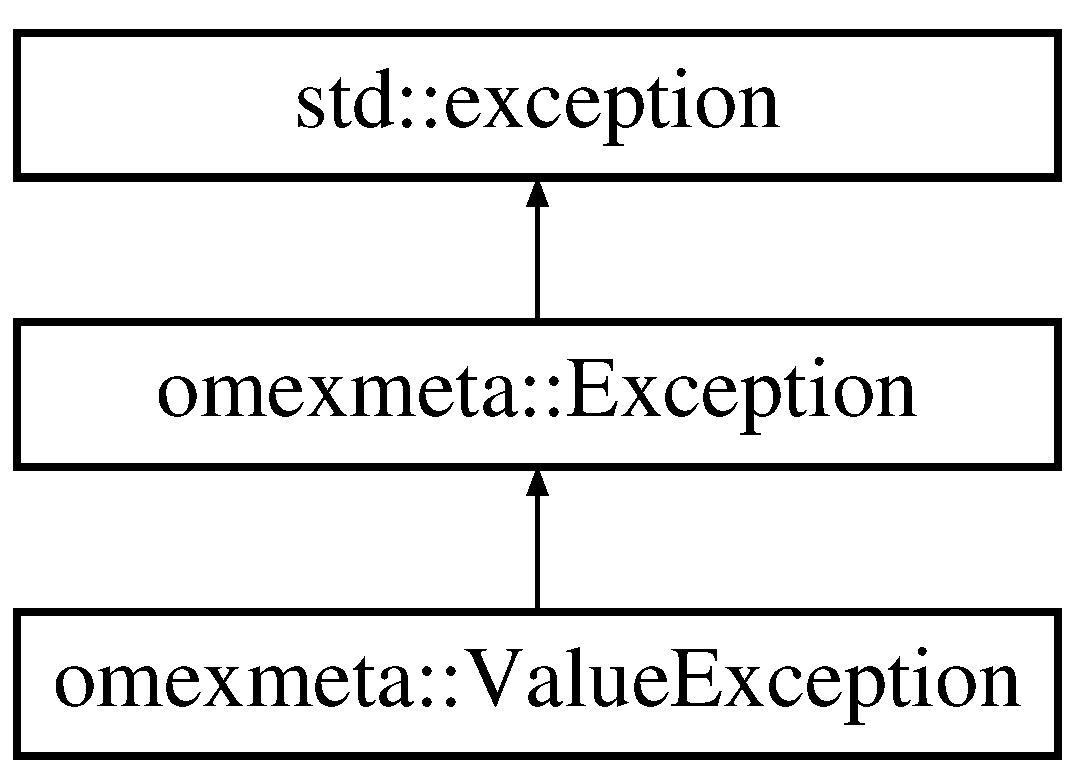
\includegraphics[height=3.000000cm]{classomexmeta_1_1ValueException}
\end{center}
\end{figure}
\doxysubsection*{Additional Inherited Members}


The documentation for this class was generated from the following file\+:\begin{DoxyCompactItemize}
\item 
src/omexmeta/Error.\+h\end{DoxyCompactItemize}

\hypertarget{classredland_1_1World}{}\section{redland\+:\+:World Class Reference}
\label{classredland_1_1World}\index{redland\+::\+World@{redland\+::\+World}}
\subsection*{Static Public Member Functions}
\begin{DoxyCompactItemize}
\item 
\mbox{\Hypertarget{classredland_1_1World_ad7618363c9b7da4c87367707c1a159d7}\label{classredland_1_1World_ad7618363c9b7da4c87367707c1a159d7}} 
static librdf\+\_\+world $\ast$ {\bfseries get\+World} ()
\item 
\mbox{\Hypertarget{classredland_1_1World_aac0ce4018279ced7b38a36d74bb10cec}\label{classredland_1_1World_aac0ce4018279ced7b38a36d74bb10cec}} 
static raptor\+\_\+world $\ast$ {\bfseries get\+Raptor} ()
\item 
\mbox{\Hypertarget{classredland_1_1World_ade64918f10ee6ee0f5b8a0cb2e01666b}\label{classredland_1_1World_ade64918f10ee6ee0f5b8a0cb2e01666b}} 
static void {\bfseries free} (librdf\+\_\+world $\ast$world)
\end{DoxyCompactItemize}


The documentation for this class was generated from the following files\+:\begin{DoxyCompactItemize}
\item 
src/redland/\+Redland\+A\+P\+I\+Wrapper/src/World.\+h\item 
src/redland/\+Redland\+A\+P\+I\+Wrapper/src/World.\+cpp\end{DoxyCompactItemize}

%--- End generated contents ---

% Index
\backmatter
\newpage
\phantomsection
\clearemptydoublepage
\addcontentsline{toc}{chapter}{Index}
\printindex

\end{document}
